\chapter{p4 = 42 (323 graphs)}
\newpage\begin{figure}
  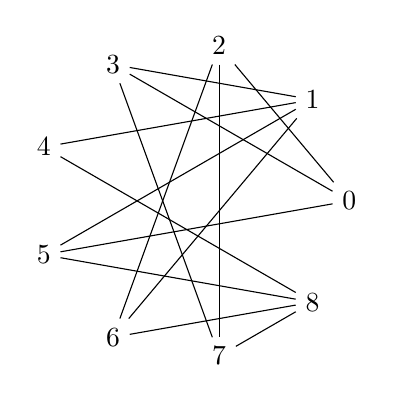
\begin{tikzpicture}
      \draw
        (0.0:2) node (0){0}
        (40.0:2) node (1){1}
        (80.0:2) node (2){2}
        (120.0:2) node (3){3}
        (160.0:2) node (4){4}
        (200.0:2) node (5){5}
        (240.0:2) node (6){6}
        (280.0:2) node (7){7}
        (320.0:2) node (8){8};
      \begin{scope}[-]
        \draw (0) to (2);
        \draw (0) to (3);
        \draw (0) to (5);
        \draw (1) to (3);
        \draw (1) to (4);
        \draw (1) to (5);
        \draw (1) to (6);
        \draw (2) to (6);
        \draw (2) to (7);
        \draw (3) to (7);
        \draw (4) to (8);
        \draw (5) to (8);
        \draw (6) to (8);
        \draw (7) to (8);
      \end{scope}
    \end{tikzpicture}
\end{figure}
\begin{itemize}
\item signature: 011010000111100000110000100001001011
\item g: Graph with 9 nodes and 14 edges
\item order: 9
\item size: 14
\item max degree: 4
\item degrees: 2,3,3,3,3,3,3,4,4
\item is tree: 0
\item is bipartite: 0
\item has bridge: 0
\item is chordal: 0
\item is complete: 0
\item min cycle basis weight: 25
\item min cycle basis size: 6
\item diameter: 3
\item radius: 2
\item is eulerian: 0
\item is planar: 0
\item number of faces: 7
\item is regular: 0
\item p3: 31
\item p4: 42
\item property hash: 105bf15f4fd1948bed471e1734d0d4dd71afaa2469e6ef2e5560f395eebb6487
\end{itemize}
\newpage
\begin{figure}
  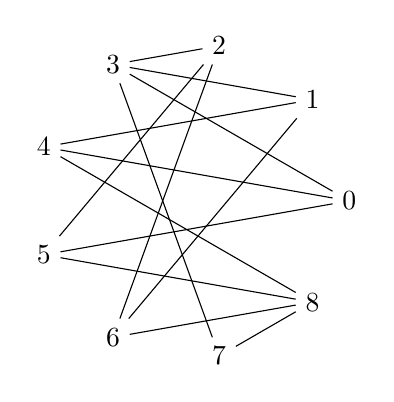
\begin{tikzpicture}
      \draw
        (0.0:2) node (0){0}
        (40.0:2) node (1){1}
        (80.0:2) node (2){2}
        (120.0:2) node (3){3}
        (160.0:2) node (4){4}
        (200.0:2) node (5){5}
        (240.0:2) node (6){6}
        (280.0:2) node (7){7}
        (320.0:2) node (8){8};
      \begin{scope}[-]
        \draw (0) to (3);
        \draw (0) to (4);
        \draw (0) to (5);
        \draw (1) to (3);
        \draw (1) to (4);
        \draw (1) to (6);
        \draw (2) to (3);
        \draw (2) to (5);
        \draw (2) to (6);
        \draw (3) to (7);
        \draw (4) to (8);
        \draw (5) to (8);
        \draw (6) to (8);
        \draw (7) to (8);
      \end{scope}
    \end{tikzpicture}
\end{figure}
\begin{itemize}
\item signature: 001110000110100101100000100001001011
\item g: Graph with 9 nodes and 14 edges
\item order: 9
\item size: 14
\item max degree: 4
\item degrees: 2,3,3,3,3,3,3,4,4
\item is tree: 0
\item is bipartite: 0
\item has bridge: 0
\item is chordal: 0
\item is complete: 0
\item min cycle basis weight: 25
\item min cycle basis size: 6
\item diameter: 3
\item radius: 2
\item is eulerian: 0
\item is planar: 0
\item number of faces: 7
\item is regular: 0
\item p3: 31
\item p4: 42
\item property hash: 105bf15f4fd1948bed471e1734d0d4dd71afaa2469e6ef2e5560f395eebb6487
\end{itemize}
\newpage
\begin{figure}
  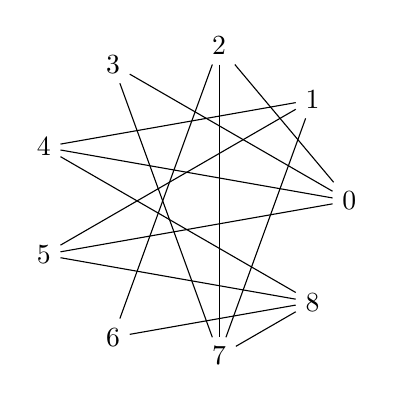
\begin{tikzpicture}
      \draw
        (0.0:2) node (0){0}
        (40.0:2) node (1){1}
        (80.0:2) node (2){2}
        (120.0:2) node (3){3}
        (160.0:2) node (4){4}
        (200.0:2) node (5){5}
        (240.0:2) node (6){6}
        (280.0:2) node (7){7}
        (320.0:2) node (8){8};
      \begin{scope}[-]
        \draw (0) to (2);
        \draw (0) to (3);
        \draw (0) to (4);
        \draw (0) to (5);
        \draw (1) to (4);
        \draw (1) to (5);
        \draw (1) to (7);
        \draw (2) to (6);
        \draw (2) to (7);
        \draw (3) to (7);
        \draw (4) to (8);
        \draw (5) to (8);
        \draw (6) to (8);
        \draw (7) to (8);
      \end{scope}
    \end{tikzpicture}
\end{figure}
\begin{itemize}
\item signature: 011110000011010000110000100001001011
\item g: Graph with 9 nodes and 14 edges
\item order: 9
\item size: 14
\item max degree: 4
\item degrees: 2,2,3,3,3,3,4,4,4
\item is tree: 0
\item is bipartite: 0
\item has bridge: 0
\item is chordal: 0
\item is complete: 0
\item min cycle basis weight: 25
\item min cycle basis size: 6
\item diameter: 3
\item radius: 2
\item is eulerian: 0
\item is planar: 0
\item number of faces: 7
\item is regular: 0
\item p3: 32
\item p4: 42
\item property hash: 7be86d856fdc6272142554dc71f3e576663e28c88c27c98878003bc89fbe053c
\end{itemize}
\newpage
\begin{figure}
  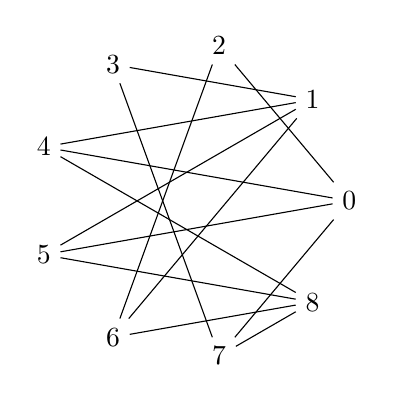
\begin{tikzpicture}
      \draw
        (0.0:2) node (0){0}
        (40.0:2) node (1){1}
        (80.0:2) node (2){2}
        (120.0:2) node (3){3}
        (160.0:2) node (4){4}
        (200.0:2) node (5){5}
        (240.0:2) node (6){6}
        (280.0:2) node (7){7}
        (320.0:2) node (8){8};
      \begin{scope}[-]
        \draw (0) to (2);
        \draw (0) to (4);
        \draw (0) to (5);
        \draw (0) to (7);
        \draw (1) to (3);
        \draw (1) to (4);
        \draw (1) to (5);
        \draw (1) to (6);
        \draw (2) to (6);
        \draw (3) to (7);
        \draw (4) to (8);
        \draw (5) to (8);
        \draw (6) to (8);
        \draw (7) to (8);
      \end{scope}
    \end{tikzpicture}
\end{figure}
\begin{itemize}
\item signature: 010110100111100000100000100001001011
\item g: Graph with 9 nodes and 14 edges
\item order: 9
\item size: 14
\item max degree: 4
\item degrees: 2,2,3,3,3,3,4,4,4
\item is tree: 0
\item is bipartite: 0
\item has bridge: 0
\item is chordal: 0
\item is complete: 0
\item min cycle basis weight: 26
\item min cycle basis size: 6
\item diameter: 3
\item radius: 2
\item is eulerian: 0
\item is planar: 0
\item number of faces: 7
\item is regular: 0
\item p3: 32
\item p4: 42
\item property hash: ce0c3098356e567c8a43025ea0d9554c880bd20caab84e9ba8859c640908beb1
\end{itemize}
\newpage
\begin{figure}
  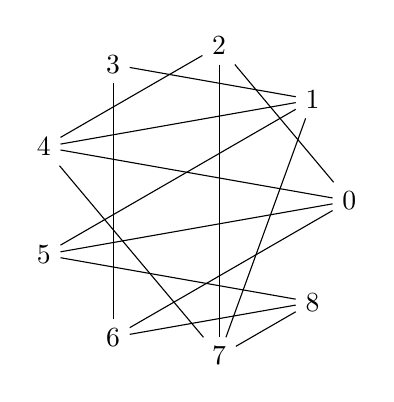
\begin{tikzpicture}
      \draw
        (0.0:2) node (0){0}
        (40.0:2) node (1){1}
        (80.0:2) node (2){2}
        (120.0:2) node (3){3}
        (160.0:2) node (4){4}
        (200.0:2) node (5){5}
        (240.0:2) node (6){6}
        (280.0:2) node (7){7}
        (320.0:2) node (8){8};
      \begin{scope}[-]
        \draw (0) to (2);
        \draw (0) to (4);
        \draw (0) to (5);
        \draw (0) to (6);
        \draw (1) to (3);
        \draw (1) to (4);
        \draw (1) to (5);
        \draw (1) to (7);
        \draw (2) to (4);
        \draw (2) to (7);
        \draw (3) to (6);
        \draw (4) to (7);
        \draw (5) to (8);
        \draw (6) to (8);
        \draw (7) to (8);
      \end{scope}
    \end{tikzpicture}
\end{figure}
\begin{itemize}
\item signature: 010111000111010010010001000010001011
\item g: Graph with 9 nodes and 15 edges
\item order: 9
\item size: 15
\item max degree: 4
\item degrees: 2,3,3,3,3,4,4,4,4
\item is tree: 0
\item is bipartite: 0
\item has bridge: 0
\item is chordal: 0
\item is complete: 0
\item min cycle basis weight: 26
\item min cycle basis size: 7
\item diameter: 3
\item radius: 2
\item is eulerian: 0
\item is planar: 0
\item number of faces: 8
\item is regular: 0
\item p3: 28
\item p4: 42
\item property hash: db0a3148a4772c77434b4025b97645776ebd508d93bdea0fa2e1c4a81086330e
\end{itemize}
\newpage
\begin{figure}
  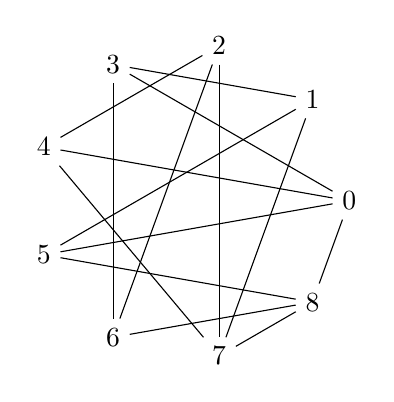
\begin{tikzpicture}
      \draw
        (0.0:2) node (0){0}
        (40.0:2) node (1){1}
        (80.0:2) node (2){2}
        (120.0:2) node (3){3}
        (160.0:2) node (4){4}
        (200.0:2) node (5){5}
        (240.0:2) node (6){6}
        (280.0:2) node (7){7}
        (320.0:2) node (8){8};
      \begin{scope}[-]
        \draw (0) to (3);
        \draw (0) to (4);
        \draw (0) to (5);
        \draw (0) to (8);
        \draw (1) to (3);
        \draw (1) to (5);
        \draw (1) to (7);
        \draw (2) to (4);
        \draw (2) to (6);
        \draw (2) to (7);
        \draw (3) to (6);
        \draw (4) to (7);
        \draw (5) to (8);
        \draw (6) to (8);
        \draw (7) to (8);
      \end{scope}
    \end{tikzpicture}
\end{figure}
\begin{itemize}
\item signature: 001110010101010010110001000010001011
\item g: Graph with 9 nodes and 15 edges
\item order: 9
\item size: 15
\item max degree: 4
\item degrees: 3,3,3,3,3,3,4,4,4
\item is tree: 0
\item is bipartite: 0
\item has bridge: 0
\item is chordal: 0
\item is complete: 0
\item min cycle basis weight: 26
\item min cycle basis size: 7
\item diameter: 3
\item radius: 2
\item is eulerian: 0
\item is planar: 0
\item number of faces: 8
\item is regular: 0
\item p3: 30
\item p4: 42
\item property hash: 36b250848c470a5bbc9677873a1f75c8a85039d66530ecb1e4c53d076396ec0b
\end{itemize}
\newpage
\begin{figure}
  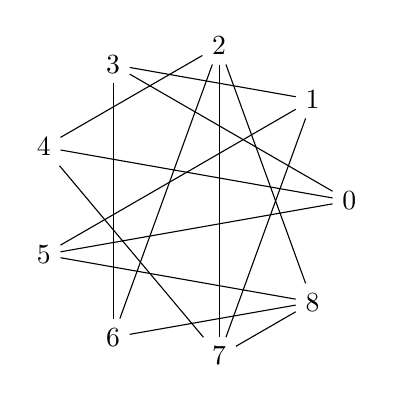
\begin{tikzpicture}
      \draw
        (0.0:2) node (0){0}
        (40.0:2) node (1){1}
        (80.0:2) node (2){2}
        (120.0:2) node (3){3}
        (160.0:2) node (4){4}
        (200.0:2) node (5){5}
        (240.0:2) node (6){6}
        (280.0:2) node (7){7}
        (320.0:2) node (8){8};
      \begin{scope}[-]
        \draw (0) to (3);
        \draw (0) to (4);
        \draw (0) to (5);
        \draw (1) to (3);
        \draw (1) to (5);
        \draw (1) to (7);
        \draw (2) to (4);
        \draw (2) to (6);
        \draw (2) to (7);
        \draw (2) to (8);
        \draw (3) to (6);
        \draw (4) to (7);
        \draw (5) to (8);
        \draw (6) to (8);
        \draw (7) to (8);
      \end{scope}
    \end{tikzpicture}
\end{figure}
\begin{itemize}
\item signature: 001110000101010010111001000010001011
\item g: Graph with 9 nodes and 15 edges
\item order: 9
\item size: 15
\item max degree: 4
\item degrees: 3,3,3,3,3,3,4,4,4
\item is tree: 0
\item is bipartite: 0
\item has bridge: 0
\item is chordal: 0
\item is complete: 0
\item min cycle basis weight: 27
\item min cycle basis size: 7
\item diameter: 2
\item radius: 2
\item is eulerian: 0
\item is planar: 0
\item number of faces: 8
\item is regular: 0
\item p3: 27
\item p4: 42
\item property hash: 0f969b5a96c8009a167e8a8440394822c346e78f10309b5f1d37f8702ccb71f7
\end{itemize}
\newpage
\begin{figure}
  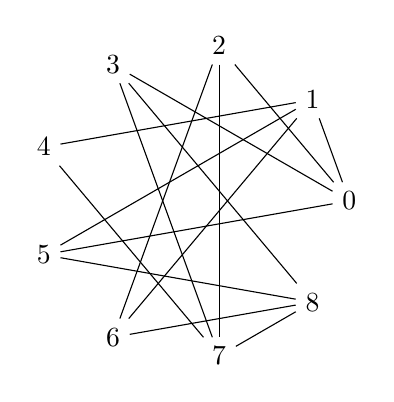
\begin{tikzpicture}
      \draw
        (0.0:2) node (0){0}
        (40.0:2) node (1){1}
        (80.0:2) node (2){2}
        (120.0:2) node (3){3}
        (160.0:2) node (4){4}
        (200.0:2) node (5){5}
        (240.0:2) node (6){6}
        (280.0:2) node (7){7}
        (320.0:2) node (8){8};
      \begin{scope}[-]
        \draw (0) to (1);
        \draw (0) to (2);
        \draw (0) to (3);
        \draw (0) to (5);
        \draw (1) to (4);
        \draw (1) to (5);
        \draw (1) to (6);
        \draw (2) to (6);
        \draw (2) to (7);
        \draw (3) to (7);
        \draw (3) to (8);
        \draw (4) to (7);
        \draw (5) to (8);
        \draw (6) to (8);
        \draw (7) to (8);
      \end{scope}
    \end{tikzpicture}
\end{figure}
\begin{itemize}
\item signature: 111010000011100000110000110010001011
\item g: Graph with 9 nodes and 15 edges
\item order: 9
\item size: 15
\item max degree: 4
\item degrees: 2,3,3,3,3,4,4,4,4
\item is tree: 0
\item is bipartite: 0
\item has bridge: 0
\item is chordal: 0
\item is complete: 0
\item min cycle basis weight: 27
\item min cycle basis size: 7
\item diameter: 2
\item radius: 2
\item is eulerian: 0
\item is planar: 0
\item number of faces: 8
\item is regular: 0
\item p3: 31
\item p4: 42
\item property hash: 8db4680f6870ed1d92a4276bd44aaed2c6c7837a32b11a889d131d33aedce953
\end{itemize}
\newpage
\begin{figure}
  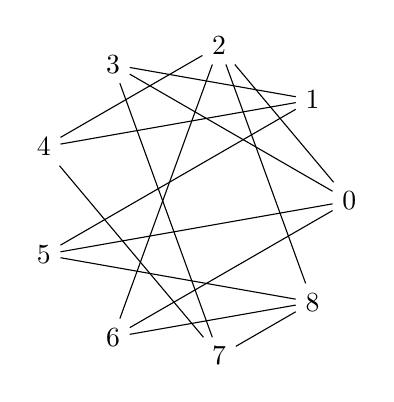
\begin{tikzpicture}
      \draw
        (0.0:2) node (0){0}
        (40.0:2) node (1){1}
        (80.0:2) node (2){2}
        (120.0:2) node (3){3}
        (160.0:2) node (4){4}
        (200.0:2) node (5){5}
        (240.0:2) node (6){6}
        (280.0:2) node (7){7}
        (320.0:2) node (8){8};
      \begin{scope}[-]
        \draw (0) to (2);
        \draw (0) to (3);
        \draw (0) to (5);
        \draw (0) to (6);
        \draw (1) to (3);
        \draw (1) to (4);
        \draw (1) to (5);
        \draw (2) to (4);
        \draw (2) to (6);
        \draw (2) to (8);
        \draw (3) to (7);
        \draw (4) to (7);
        \draw (5) to (8);
        \draw (6) to (8);
        \draw (7) to (8);
      \end{scope}
    \end{tikzpicture}
\end{figure}
\begin{itemize}
\item signature: 011011000111000010101000100010001011
\item g: Graph with 9 nodes and 15 edges
\item order: 9
\item size: 15
\item max degree: 4
\item degrees: 3,3,3,3,3,3,4,4,4
\item is tree: 0
\item is bipartite: 0
\item has bridge: 0
\item is chordal: 0
\item is complete: 0
\item min cycle basis weight: 27
\item min cycle basis size: 7
\item diameter: 3
\item radius: 2
\item is eulerian: 0
\item is planar: 0
\item number of faces: 8
\item is regular: 0
\item p3: 30
\item p4: 42
\item property hash: cf96fe14672fd17e2cd00fec91aac8fe18ee35e3ddb1e349a8b4800e325d7f20
\end{itemize}
\newpage
\begin{figure}
  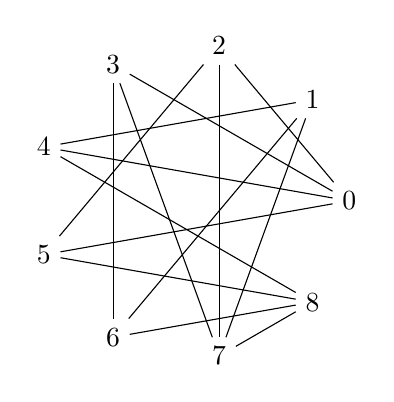
\begin{tikzpicture}
      \draw
        (0.0:2) node (0){0}
        (40.0:2) node (1){1}
        (80.0:2) node (2){2}
        (120.0:2) node (3){3}
        (160.0:2) node (4){4}
        (200.0:2) node (5){5}
        (240.0:2) node (6){6}
        (280.0:2) node (7){7}
        (320.0:2) node (8){8};
      \begin{scope}[-]
        \draw (0) to (2);
        \draw (0) to (3);
        \draw (0) to (4);
        \draw (0) to (5);
        \draw (1) to (4);
        \draw (1) to (6);
        \draw (1) to (7);
        \draw (2) to (5);
        \draw (2) to (7);
        \draw (3) to (6);
        \draw (3) to (7);
        \draw (4) to (8);
        \draw (5) to (8);
        \draw (6) to (8);
        \draw (7) to (8);
      \end{scope}
    \end{tikzpicture}
\end{figure}
\begin{itemize}
\item signature: 011110000010110001010001100001001011
\item g: Graph with 9 nodes and 15 edges
\item order: 9
\item size: 15
\item max degree: 4
\item degrees: 3,3,3,3,3,3,4,4,4
\item is tree: 0
\item is bipartite: 0
\item has bridge: 0
\item is chordal: 0
\item is complete: 0
\item min cycle basis weight: 27
\item min cycle basis size: 7
\item diameter: 3
\item radius: 2
\item is eulerian: 0
\item is planar: 0
\item number of faces: 8
\item is regular: 0
\item p3: 33
\item p4: 42
\item property hash: a28e48c607defa1ed88befc30929a5cca099bb1321a23df02dd8868878d02b4d
\end{itemize}
\newpage
\begin{figure}
  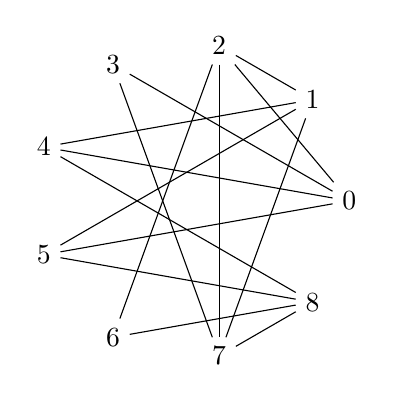
\begin{tikzpicture}
      \draw
        (0.0:2) node (0){0}
        (40.0:2) node (1){1}
        (80.0:2) node (2){2}
        (120.0:2) node (3){3}
        (160.0:2) node (4){4}
        (200.0:2) node (5){5}
        (240.0:2) node (6){6}
        (280.0:2) node (7){7}
        (320.0:2) node (8){8};
      \begin{scope}[-]
        \draw (0) to (2);
        \draw (0) to (3);
        \draw (0) to (4);
        \draw (0) to (5);
        \draw (1) to (2);
        \draw (1) to (4);
        \draw (1) to (5);
        \draw (1) to (7);
        \draw (2) to (6);
        \draw (2) to (7);
        \draw (3) to (7);
        \draw (4) to (8);
        \draw (5) to (8);
        \draw (6) to (8);
        \draw (7) to (8);
      \end{scope}
    \end{tikzpicture}
\end{figure}
\begin{itemize}
\item signature: 011110001011010000110000100001001011
\item g: Graph with 9 nodes and 15 edges
\item order: 9
\item size: 15
\item max degree: 4
\item degrees: 2,2,3,3,4,4,4,4,4
\item is tree: 0
\item is bipartite: 0
\item has bridge: 0
\item is chordal: 0
\item is complete: 0
\item min cycle basis weight: 27
\item min cycle basis size: 7
\item diameter: 3
\item radius: 2
\item is eulerian: 0
\item is planar: 0
\item number of faces: 8
\item is regular: 0
\item p3: 35
\item p4: 42
\item property hash: 2f9f25e5aedb63d0c00f448ad83f0e633df183af574b0ffd5ae74848b3de5052
\end{itemize}
\newpage
\begin{figure}
  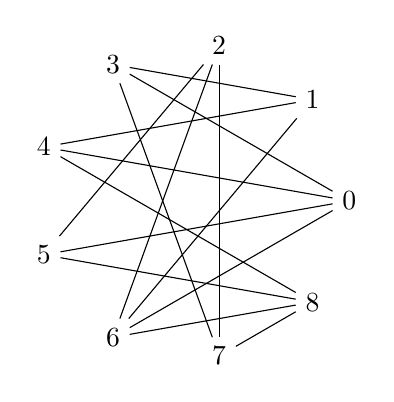
\begin{tikzpicture}
      \draw
        (0.0:2) node (0){0}
        (40.0:2) node (1){1}
        (80.0:2) node (2){2}
        (120.0:2) node (3){3}
        (160.0:2) node (4){4}
        (200.0:2) node (5){5}
        (240.0:2) node (6){6}
        (280.0:2) node (7){7}
        (320.0:2) node (8){8};
      \begin{scope}[-]
        \draw (0) to (3);
        \draw (0) to (4);
        \draw (0) to (5);
        \draw (0) to (6);
        \draw (1) to (3);
        \draw (1) to (4);
        \draw (1) to (6);
        \draw (2) to (5);
        \draw (2) to (6);
        \draw (2) to (7);
        \draw (3) to (7);
        \draw (4) to (8);
        \draw (5) to (8);
        \draw (6) to (8);
        \draw (7) to (8);
      \end{scope}
    \end{tikzpicture}
\end{figure}
\begin{itemize}
\item signature: 001111000110100001110000100001001011
\item g: Graph with 9 nodes and 15 edges
\item order: 9
\item size: 15
\item max degree: 4
\item degrees: 3,3,3,3,3,3,4,4,4
\item is tree: 0
\item is bipartite: 0
\item has bridge: 0
\item is chordal: 0
\item is complete: 0
\item min cycle basis weight: 29
\item min cycle basis size: 7
\item diameter: 3
\item radius: 2
\item is eulerian: 0
\item is planar: 0
\item number of faces: 8
\item is regular: 0
\item p3: 36
\item p4: 42
\item property hash: d3d394c2561e85ad4ff50584170aa2db5ffada45ffa8be75b02c06309395dff7
\end{itemize}
\newpage
\begin{figure}
  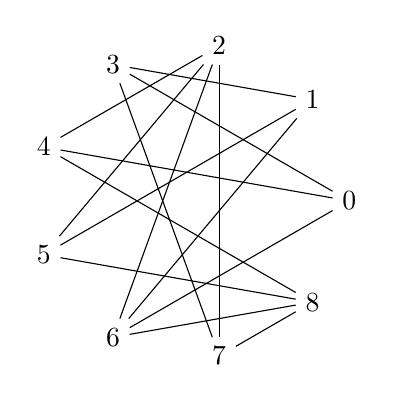
\begin{tikzpicture}
      \draw
        (0.0:2) node (0){0}
        (40.0:2) node (1){1}
        (80.0:2) node (2){2}
        (120.0:2) node (3){3}
        (160.0:2) node (4){4}
        (200.0:2) node (5){5}
        (240.0:2) node (6){6}
        (280.0:2) node (7){7}
        (320.0:2) node (8){8};
      \begin{scope}[-]
        \draw (0) to (3);
        \draw (0) to (4);
        \draw (0) to (6);
        \draw (1) to (3);
        \draw (1) to (5);
        \draw (1) to (6);
        \draw (2) to (4);
        \draw (2) to (5);
        \draw (2) to (6);
        \draw (2) to (7);
        \draw (3) to (7);
        \draw (4) to (8);
        \draw (5) to (8);
        \draw (6) to (8);
        \draw (7) to (8);
      \end{scope}
    \end{tikzpicture}
\end{figure}
\begin{itemize}
\item signature: 001101000101100011110000100001001011
\item g: Graph with 9 nodes and 15 edges
\item order: 9
\item size: 15
\item max degree: 4
\item degrees: 3,3,3,3,3,3,4,4,4
\item is tree: 0
\item is bipartite: 0
\item has bridge: 0
\item is chordal: 0
\item is complete: 0
\item min cycle basis weight: 29
\item min cycle basis size: 7
\item diameter: 3
\item radius: 2
\item is eulerian: 0
\item is planar: 0
\item number of faces: 8
\item is regular: 0
\item p3: 36
\item p4: 42
\item property hash: d3d394c2561e85ad4ff50584170aa2db5ffada45ffa8be75b02c06309395dff7
\end{itemize}
\newpage
\begin{figure}
  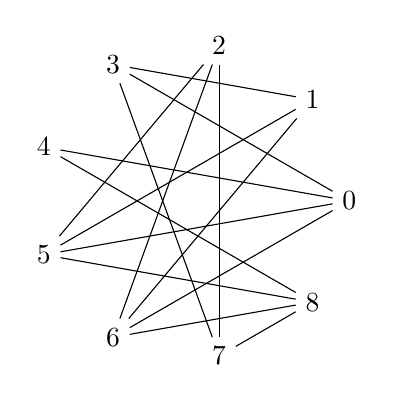
\begin{tikzpicture}
      \draw
        (0.0:2) node (0){0}
        (40.0:2) node (1){1}
        (80.0:2) node (2){2}
        (120.0:2) node (3){3}
        (160.0:2) node (4){4}
        (200.0:2) node (5){5}
        (240.0:2) node (6){6}
        (280.0:2) node (7){7}
        (320.0:2) node (8){8};
      \begin{scope}[-]
        \draw (0) to (3);
        \draw (0) to (4);
        \draw (0) to (5);
        \draw (0) to (6);
        \draw (1) to (3);
        \draw (1) to (5);
        \draw (1) to (6);
        \draw (2) to (5);
        \draw (2) to (6);
        \draw (2) to (7);
        \draw (3) to (7);
        \draw (4) to (8);
        \draw (5) to (8);
        \draw (6) to (8);
        \draw (7) to (8);
      \end{scope}
    \end{tikzpicture}
\end{figure}
\begin{itemize}
\item signature: 001111000101100001110000100001001011
\item g: Graph with 9 nodes and 15 edges
\item order: 9
\item size: 15
\item max degree: 4
\item degrees: 2,3,3,3,3,4,4,4,4
\item is tree: 0
\item is bipartite: 0
\item has bridge: 0
\item is chordal: 0
\item is complete: 0
\item min cycle basis weight: 29
\item min cycle basis size: 7
\item diameter: 3
\item radius: 2
\item is eulerian: 0
\item is planar: 0
\item number of faces: 8
\item is regular: 0
\item p3: 37
\item p4: 42
\item property hash: 667a6ba50a2d2cb17b18d3224207b6598422e3c0c5dacf8c3f1b505e504633de
\end{itemize}
\newpage
\begin{figure}
  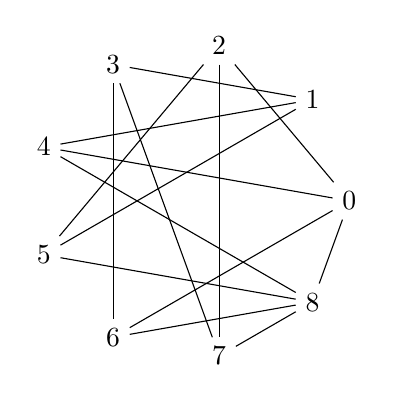
\begin{tikzpicture}
      \draw
        (0.0:2) node (0){0}
        (40.0:2) node (1){1}
        (80.0:2) node (2){2}
        (120.0:2) node (3){3}
        (160.0:2) node (4){4}
        (200.0:2) node (5){5}
        (240.0:2) node (6){6}
        (280.0:2) node (7){7}
        (320.0:2) node (8){8};
      \begin{scope}[-]
        \draw (0) to (2);
        \draw (0) to (4);
        \draw (0) to (6);
        \draw (0) to (8);
        \draw (1) to (3);
        \draw (1) to (4);
        \draw (1) to (5);
        \draw (2) to (5);
        \draw (2) to (7);
        \draw (3) to (6);
        \draw (3) to (7);
        \draw (4) to (8);
        \draw (5) to (8);
        \draw (6) to (8);
        \draw (7) to (8);
      \end{scope}
    \end{tikzpicture}
\end{figure}
\begin{itemize}
\item signature: 010101010111000001010001100001001011
\item g: Graph with 9 nodes and 15 edges
\item order: 9
\item size: 15
\item max degree: 5
\item degrees: 3,3,3,3,3,3,3,4,5
\item is tree: 0
\item is bipartite: 0
\item has bridge: 0
\item is chordal: 0
\item is complete: 0
\item min cycle basis weight: 27
\item min cycle basis size: 7
\item diameter: 2
\item radius: 2
\item is eulerian: 0
\item is planar: 0
\item number of faces: 8
\item is regular: 0
\item p3: 31
\item p4: 42
\item property hash: 5e1880a4b4dcb25376db6ee98ff3b2d6d892900eaa2ae2cc483d8841f06e75b4
\end{itemize}
\newpage
\begin{figure}
  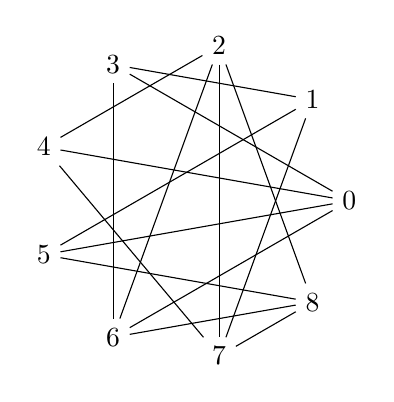
\begin{tikzpicture}
      \draw
        (0.0:2) node (0){0}
        (40.0:2) node (1){1}
        (80.0:2) node (2){2}
        (120.0:2) node (3){3}
        (160.0:2) node (4){4}
        (200.0:2) node (5){5}
        (240.0:2) node (6){6}
        (280.0:2) node (7){7}
        (320.0:2) node (8){8};
      \begin{scope}[-]
        \draw (0) to (3);
        \draw (0) to (4);
        \draw (0) to (5);
        \draw (0) to (6);
        \draw (1) to (3);
        \draw (1) to (5);
        \draw (1) to (7);
        \draw (2) to (4);
        \draw (2) to (6);
        \draw (2) to (7);
        \draw (2) to (8);
        \draw (3) to (6);
        \draw (4) to (7);
        \draw (5) to (8);
        \draw (6) to (8);
        \draw (7) to (8);
      \end{scope}
    \end{tikzpicture}
\end{figure}
\begin{itemize}
\item signature: 001111000101010010111001000010001011
\item g: Graph with 9 nodes and 16 edges
\item order: 9
\item size: 16
\item max degree: 4
\item degrees: 3,3,3,3,4,4,4,4,4
\item is tree: 0
\item is bipartite: 0
\item has bridge: 0
\item is chordal: 0
\item is complete: 0
\item min cycle basis weight: 28
\item min cycle basis size: 8
\item diameter: 2
\item radius: 2
\item is eulerian: 0
\item is planar: 0
\item number of faces: 9
\item is regular: 0
\item p3: 30
\item p4: 42
\item property hash: c874b5912bcd089c589a0fcfb6aba2f5cb24d216c57d8c5ca03eb33c5e0eacd8
\end{itemize}
\newpage
\begin{figure}
  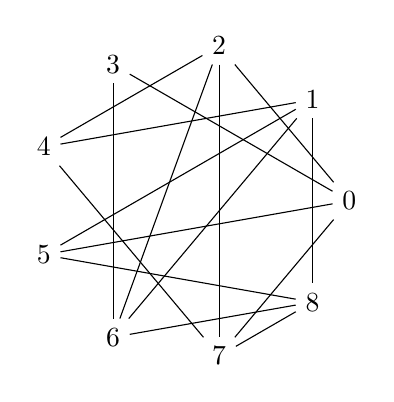
\begin{tikzpicture}
      \draw
        (0.0:2) node (0){0}
        (40.0:2) node (1){1}
        (80.0:2) node (2){2}
        (120.0:2) node (3){3}
        (160.0:2) node (4){4}
        (200.0:2) node (5){5}
        (240.0:2) node (6){6}
        (280.0:2) node (7){7}
        (320.0:2) node (8){8};
      \begin{scope}[-]
        \draw (0) to (2);
        \draw (0) to (3);
        \draw (0) to (5);
        \draw (0) to (7);
        \draw (1) to (4);
        \draw (1) to (5);
        \draw (1) to (6);
        \draw (1) to (8);
        \draw (2) to (4);
        \draw (2) to (6);
        \draw (2) to (7);
        \draw (3) to (6);
        \draw (4) to (7);
        \draw (5) to (8);
        \draw (6) to (8);
        \draw (7) to (8);
      \end{scope}
    \end{tikzpicture}
\end{figure}
\begin{itemize}
\item signature: 011010100011101010110001000010001011
\item g: Graph with 9 nodes and 16 edges
\item order: 9
\item size: 16
\item max degree: 4
\item degrees: 2,3,3,4,4,4,4,4,4
\item is tree: 0
\item is bipartite: 0
\item has bridge: 0
\item is chordal: 0
\item is complete: 0
\item min cycle basis weight: 28
\item min cycle basis size: 8
\item diameter: 3
\item radius: 2
\item is eulerian: 0
\item is planar: 0
\item number of faces: 9
\item is regular: 0
\item p3: 31
\item p4: 42
\item property hash: aaa428bf7a5861f64adbaf4b9fec81547b56bb6db97b0cb646bdf2bfcda4ebf5
\end{itemize}
\newpage
\begin{figure}
  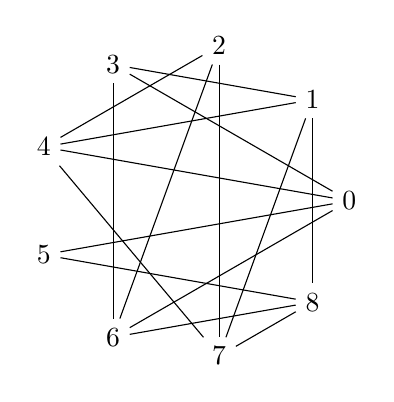
\begin{tikzpicture}
      \draw
        (0.0:2) node (0){0}
        (40.0:2) node (1){1}
        (80.0:2) node (2){2}
        (120.0:2) node (3){3}
        (160.0:2) node (4){4}
        (200.0:2) node (5){5}
        (240.0:2) node (6){6}
        (280.0:2) node (7){7}
        (320.0:2) node (8){8};
      \begin{scope}[-]
        \draw (0) to (3);
        \draw (0) to (4);
        \draw (0) to (5);
        \draw (0) to (6);
        \draw (1) to (3);
        \draw (1) to (4);
        \draw (1) to (7);
        \draw (1) to (8);
        \draw (2) to (4);
        \draw (2) to (6);
        \draw (2) to (7);
        \draw (3) to (6);
        \draw (4) to (7);
        \draw (5) to (8);
        \draw (6) to (8);
        \draw (7) to (8);
      \end{scope}
    \end{tikzpicture}
\end{figure}
\begin{itemize}
\item signature: 001111000110011010110001000010001011
\item g: Graph with 9 nodes and 16 edges
\item order: 9
\item size: 16
\item max degree: 4
\item degrees: 2,3,3,4,4,4,4,4,4
\item is tree: 0
\item is bipartite: 0
\item has bridge: 0
\item is chordal: 0
\item is complete: 0
\item min cycle basis weight: 28
\item min cycle basis size: 8
\item diameter: 3
\item radius: 2
\item is eulerian: 0
\item is planar: 0
\item number of faces: 9
\item is regular: 0
\item p3: 31
\item p4: 42
\item property hash: aaa428bf7a5861f64adbaf4b9fec81547b56bb6db97b0cb646bdf2bfcda4ebf5
\end{itemize}
\newpage
\begin{figure}
  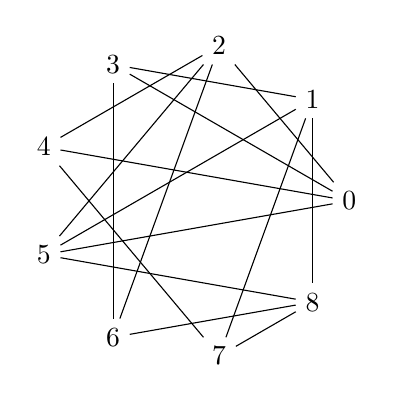
\begin{tikzpicture}
      \draw
        (0.0:2) node (0){0}
        (40.0:2) node (1){1}
        (80.0:2) node (2){2}
        (120.0:2) node (3){3}
        (160.0:2) node (4){4}
        (200.0:2) node (5){5}
        (240.0:2) node (6){6}
        (280.0:2) node (7){7}
        (320.0:2) node (8){8};
      \begin{scope}[-]
        \draw (0) to (2);
        \draw (0) to (3);
        \draw (0) to (4);
        \draw (0) to (5);
        \draw (1) to (3);
        \draw (1) to (5);
        \draw (1) to (7);
        \draw (1) to (8);
        \draw (2) to (4);
        \draw (2) to (5);
        \draw (2) to (6);
        \draw (3) to (6);
        \draw (4) to (7);
        \draw (5) to (8);
        \draw (6) to (8);
        \draw (7) to (8);
      \end{scope}
    \end{tikzpicture}
\end{figure}
\begin{itemize}
\item signature: 011110000101011011100001000010001011
\item g: Graph with 9 nodes and 16 edges
\item order: 9
\item size: 16
\item max degree: 4
\item degrees: 3,3,3,3,4,4,4,4,4
\item is tree: 0
\item is bipartite: 0
\item has bridge: 0
\item is chordal: 0
\item is complete: 0
\item min cycle basis weight: 29
\item min cycle basis size: 8
\item diameter: 2
\item radius: 2
\item is eulerian: 0
\item is planar: 0
\item number of faces: 9
\item is regular: 0
\item p3: 30
\item p4: 42
\item property hash: 263586ca8f0bea04a1ae75d70555ba5a684e6d836cc2ac442b1e731e6ed50c8f
\end{itemize}
\newpage
\begin{figure}
  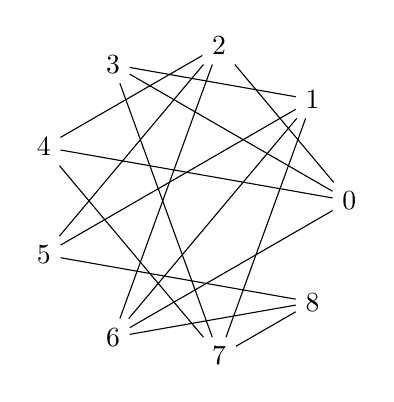
\begin{tikzpicture}
      \draw
        (0.0:2) node (0){0}
        (40.0:2) node (1){1}
        (80.0:2) node (2){2}
        (120.0:2) node (3){3}
        (160.0:2) node (4){4}
        (200.0:2) node (5){5}
        (240.0:2) node (6){6}
        (280.0:2) node (7){7}
        (320.0:2) node (8){8};
      \begin{scope}[-]
        \draw (0) to (2);
        \draw (0) to (3);
        \draw (0) to (4);
        \draw (0) to (6);
        \draw (1) to (3);
        \draw (1) to (5);
        \draw (1) to (6);
        \draw (1) to (7);
        \draw (2) to (4);
        \draw (2) to (5);
        \draw (2) to (6);
        \draw (3) to (7);
        \draw (4) to (7);
        \draw (5) to (8);
        \draw (6) to (8);
        \draw (7) to (8);
      \end{scope}
    \end{tikzpicture}
\end{figure}
\begin{itemize}
\item signature: 011101000101110011100000100010001011
\item g: Graph with 9 nodes and 16 edges
\item order: 9
\item size: 16
\item max degree: 4
\item degrees: 3,3,3,3,4,4,4,4,4
\item is tree: 0
\item is bipartite: 0
\item has bridge: 0
\item is chordal: 0
\item is complete: 0
\item min cycle basis weight: 29
\item min cycle basis size: 8
\item diameter: 2
\item radius: 2
\item is eulerian: 0
\item is planar: 0
\item number of faces: 9
\item is regular: 0
\item p3: 33
\item p4: 42
\item property hash: 0ff8dd29a8c424a80248dbcebb281f1566cbf0e624bcd026cebfec994887abce
\end{itemize}
\newpage
\begin{figure}
  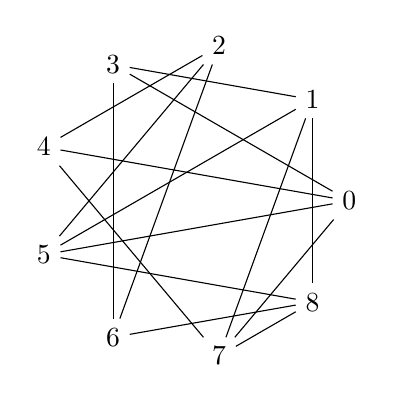
\begin{tikzpicture}
      \draw
        (0.0:2) node (0){0}
        (40.0:2) node (1){1}
        (80.0:2) node (2){2}
        (120.0:2) node (3){3}
        (160.0:2) node (4){4}
        (200.0:2) node (5){5}
        (240.0:2) node (6){6}
        (280.0:2) node (7){7}
        (320.0:2) node (8){8};
      \begin{scope}[-]
        \draw (0) to (3);
        \draw (0) to (4);
        \draw (0) to (5);
        \draw (0) to (7);
        \draw (1) to (3);
        \draw (1) to (5);
        \draw (1) to (7);
        \draw (1) to (8);
        \draw (2) to (4);
        \draw (2) to (5);
        \draw (2) to (6);
        \draw (3) to (6);
        \draw (4) to (7);
        \draw (5) to (8);
        \draw (6) to (8);
        \draw (7) to (8);
      \end{scope}
    \end{tikzpicture}
\end{figure}
\begin{itemize}
\item signature: 001110100101011011100001000010001011
\item g: Graph with 9 nodes and 16 edges
\item order: 9
\item size: 16
\item max degree: 4
\item degrees: 3,3,3,3,4,4,4,4,4
\item is tree: 0
\item is bipartite: 0
\item has bridge: 0
\item is chordal: 0
\item is complete: 0
\item min cycle basis weight: 29
\item min cycle basis size: 8
\item diameter: 2
\item radius: 2
\item is eulerian: 0
\item is planar: 0
\item number of faces: 9
\item is regular: 0
\item p3: 33
\item p4: 42
\item property hash: 0ff8dd29a8c424a80248dbcebb281f1566cbf0e624bcd026cebfec994887abce
\end{itemize}
\newpage
\begin{figure}
  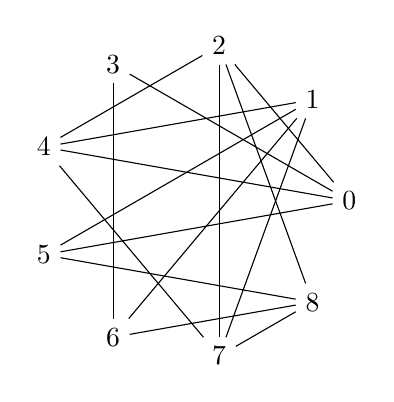
\begin{tikzpicture}
      \draw
        (0.0:2) node (0){0}
        (40.0:2) node (1){1}
        (80.0:2) node (2){2}
        (120.0:2) node (3){3}
        (160.0:2) node (4){4}
        (200.0:2) node (5){5}
        (240.0:2) node (6){6}
        (280.0:2) node (7){7}
        (320.0:2) node (8){8};
      \begin{scope}[-]
        \draw (0) to (2);
        \draw (0) to (3);
        \draw (0) to (4);
        \draw (0) to (5);
        \draw (1) to (4);
        \draw (1) to (5);
        \draw (1) to (6);
        \draw (1) to (7);
        \draw (2) to (4);
        \draw (2) to (7);
        \draw (2) to (8);
        \draw (3) to (6);
        \draw (4) to (7);
        \draw (5) to (8);
        \draw (6) to (8);
        \draw (7) to (8);
      \end{scope}
    \end{tikzpicture}
\end{figure}
\begin{itemize}
\item signature: 011110000011110010011001000010001011
\item g: Graph with 9 nodes and 16 edges
\item order: 9
\item size: 16
\item max degree: 4
\item degrees: 2,3,3,4,4,4,4,4,4
\item is tree: 0
\item is bipartite: 0
\item has bridge: 0
\item is chordal: 0
\item is complete: 0
\item min cycle basis weight: 29
\item min cycle basis size: 8
\item diameter: 3
\item radius: 2
\item is eulerian: 0
\item is planar: 0
\item number of faces: 9
\item is regular: 0
\item p3: 31
\item p4: 42
\item property hash: e961c624bbbe2736bb1f07465da23831355df29e040ce0ef2ec4130c4f3c88cd
\end{itemize}
\newpage
\begin{figure}
  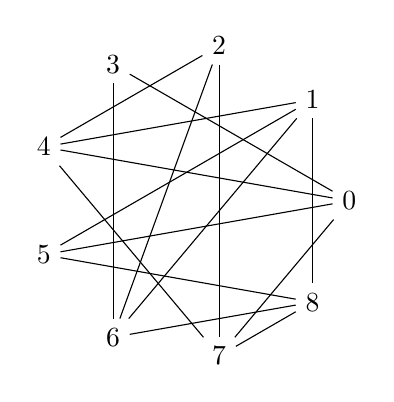
\begin{tikzpicture}
      \draw
        (0.0:2) node (0){0}
        (40.0:2) node (1){1}
        (80.0:2) node (2){2}
        (120.0:2) node (3){3}
        (160.0:2) node (4){4}
        (200.0:2) node (5){5}
        (240.0:2) node (6){6}
        (280.0:2) node (7){7}
        (320.0:2) node (8){8};
      \begin{scope}[-]
        \draw (0) to (3);
        \draw (0) to (4);
        \draw (0) to (5);
        \draw (0) to (7);
        \draw (1) to (4);
        \draw (1) to (5);
        \draw (1) to (6);
        \draw (1) to (8);
        \draw (2) to (4);
        \draw (2) to (6);
        \draw (2) to (7);
        \draw (3) to (6);
        \draw (4) to (7);
        \draw (5) to (8);
        \draw (6) to (8);
        \draw (7) to (8);
      \end{scope}
    \end{tikzpicture}
\end{figure}
\begin{itemize}
\item signature: 001110100011101010110001000010001011
\item g: Graph with 9 nodes and 16 edges
\item order: 9
\item size: 16
\item max degree: 4
\item degrees: 2,3,3,4,4,4,4,4,4
\item is tree: 0
\item is bipartite: 0
\item has bridge: 0
\item is chordal: 0
\item is complete: 0
\item min cycle basis weight: 29
\item min cycle basis size: 8
\item diameter: 3
\item radius: 2
\item is eulerian: 0
\item is planar: 0
\item number of faces: 9
\item is regular: 0
\item p3: 31
\item p4: 42
\item property hash: e961c624bbbe2736bb1f07465da23831355df29e040ce0ef2ec4130c4f3c88cd
\end{itemize}
\newpage
\begin{figure}
  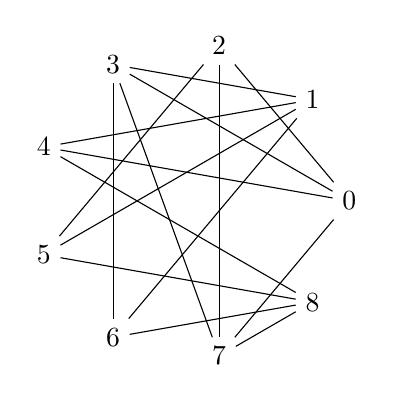
\begin{tikzpicture}
      \draw
        (0.0:2) node (0){0}
        (40.0:2) node (1){1}
        (80.0:2) node (2){2}
        (120.0:2) node (3){3}
        (160.0:2) node (4){4}
        (200.0:2) node (5){5}
        (240.0:2) node (6){6}
        (280.0:2) node (7){7}
        (320.0:2) node (8){8};
      \begin{scope}[-]
        \draw (0) to (2);
        \draw (0) to (3);
        \draw (0) to (4);
        \draw (0) to (7);
        \draw (1) to (3);
        \draw (1) to (4);
        \draw (1) to (5);
        \draw (1) to (6);
        \draw (2) to (5);
        \draw (2) to (7);
        \draw (3) to (6);
        \draw (3) to (7);
        \draw (4) to (8);
        \draw (5) to (8);
        \draw (6) to (8);
        \draw (7) to (8);
      \end{scope}
    \end{tikzpicture}
\end{figure}
\begin{itemize}
\item signature: 011100100111100001010001100001001011
\item g: Graph with 9 nodes and 16 edges
\item order: 9
\item size: 16
\item max degree: 4
\item degrees: 3,3,3,3,4,4,4,4,4
\item is tree: 0
\item is bipartite: 0
\item has bridge: 0
\item is chordal: 0
\item is complete: 0
\item min cycle basis weight: 29
\item min cycle basis size: 8
\item diameter: 3
\item radius: 2
\item is eulerian: 0
\item is planar: 0
\item number of faces: 9
\item is regular: 0
\item p3: 33
\item p4: 42
\item property hash: 87e3cc8606aef5d325970a90858515e91b8ed7560e7202e6048758eaac2d95a6
\end{itemize}
\newpage
\begin{figure}
  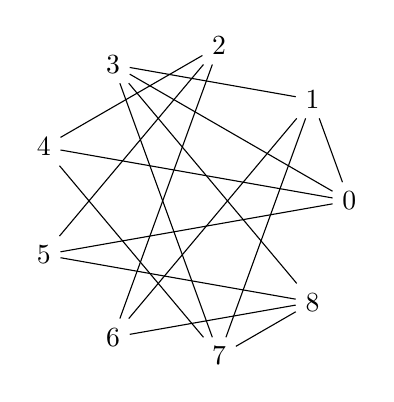
\begin{tikzpicture}
      \draw
        (0.0:2) node (0){0}
        (40.0:2) node (1){1}
        (80.0:2) node (2){2}
        (120.0:2) node (3){3}
        (160.0:2) node (4){4}
        (200.0:2) node (5){5}
        (240.0:2) node (6){6}
        (280.0:2) node (7){7}
        (320.0:2) node (8){8};
      \begin{scope}[-]
        \draw (0) to (1);
        \draw (0) to (3);
        \draw (0) to (4);
        \draw (0) to (5);
        \draw (1) to (3);
        \draw (1) to (6);
        \draw (1) to (7);
        \draw (2) to (4);
        \draw (2) to (5);
        \draw (2) to (6);
        \draw (3) to (7);
        \draw (3) to (8);
        \draw (4) to (7);
        \draw (5) to (8);
        \draw (6) to (8);
        \draw (7) to (8);
      \end{scope}
    \end{tikzpicture}
\end{figure}
\begin{itemize}
\item signature: 101110000100110011100000110010001011
\item g: Graph with 9 nodes and 16 edges
\item order: 9
\item size: 16
\item max degree: 4
\item degrees: 3,3,3,3,4,4,4,4,4
\item is tree: 0
\item is bipartite: 0
\item has bridge: 0
\item is chordal: 0
\item is complete: 0
\item min cycle basis weight: 29
\item min cycle basis size: 8
\item diameter: 3
\item radius: 2
\item is eulerian: 0
\item is planar: 0
\item number of faces: 9
\item is regular: 0
\item p3: 33
\item p4: 42
\item property hash: 87e3cc8606aef5d325970a90858515e91b8ed7560e7202e6048758eaac2d95a6
\end{itemize}
\newpage
\begin{figure}
  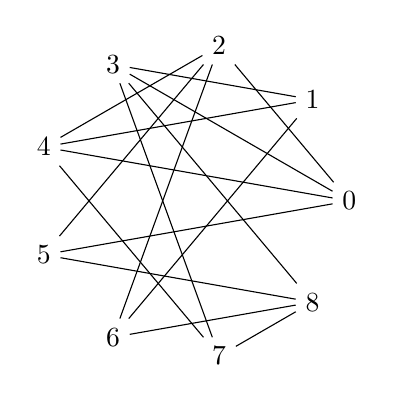
\begin{tikzpicture}
      \draw
        (0.0:2) node (0){0}
        (40.0:2) node (1){1}
        (80.0:2) node (2){2}
        (120.0:2) node (3){3}
        (160.0:2) node (4){4}
        (200.0:2) node (5){5}
        (240.0:2) node (6){6}
        (280.0:2) node (7){7}
        (320.0:2) node (8){8};
      \begin{scope}[-]
        \draw (0) to (2);
        \draw (0) to (3);
        \draw (0) to (4);
        \draw (0) to (5);
        \draw (1) to (3);
        \draw (1) to (4);
        \draw (1) to (6);
        \draw (2) to (4);
        \draw (2) to (5);
        \draw (2) to (6);
        \draw (3) to (7);
        \draw (3) to (8);
        \draw (4) to (7);
        \draw (5) to (8);
        \draw (6) to (8);
        \draw (7) to (8);
      \end{scope}
    \end{tikzpicture}
\end{figure}
\begin{itemize}
\item signature: 011110000110100011100000110010001011
\item g: Graph with 9 nodes and 16 edges
\item order: 9
\item size: 16
\item max degree: 4
\item degrees: 3,3,3,3,4,4,4,4,4
\item is tree: 0
\item is bipartite: 0
\item has bridge: 0
\item is chordal: 0
\item is complete: 0
\item min cycle basis weight: 29
\item min cycle basis size: 8
\item diameter: 3
\item radius: 2
\item is eulerian: 0
\item is planar: 0
\item number of faces: 9
\item is regular: 0
\item p3: 33
\item p4: 42
\item property hash: 87e3cc8606aef5d325970a90858515e91b8ed7560e7202e6048758eaac2d95a6
\end{itemize}
\newpage
\begin{figure}
  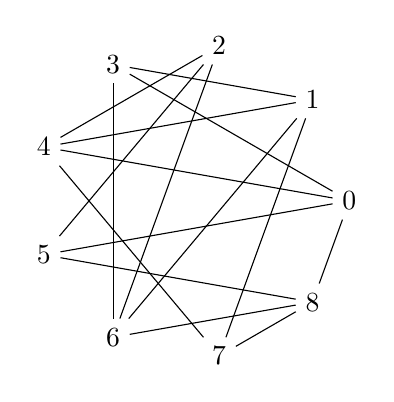
\begin{tikzpicture}
      \draw
        (0.0:2) node (0){0}
        (40.0:2) node (1){1}
        (80.0:2) node (2){2}
        (120.0:2) node (3){3}
        (160.0:2) node (4){4}
        (200.0:2) node (5){5}
        (240.0:2) node (6){6}
        (280.0:2) node (7){7}
        (320.0:2) node (8){8};
      \begin{scope}[-]
        \draw (0) to (3);
        \draw (0) to (4);
        \draw (0) to (5);
        \draw (0) to (8);
        \draw (1) to (3);
        \draw (1) to (4);
        \draw (1) to (6);
        \draw (1) to (7);
        \draw (2) to (4);
        \draw (2) to (5);
        \draw (2) to (6);
        \draw (3) to (6);
        \draw (4) to (7);
        \draw (5) to (8);
        \draw (6) to (8);
        \draw (7) to (8);
      \end{scope}
    \end{tikzpicture}
\end{figure}
\begin{itemize}
\item signature: 001110010110110011100001000010001011
\item g: Graph with 9 nodes and 16 edges
\item order: 9
\item size: 16
\item max degree: 4
\item degrees: 3,3,3,3,4,4,4,4,4
\item is tree: 0
\item is bipartite: 0
\item has bridge: 0
\item is chordal: 0
\item is complete: 0
\item min cycle basis weight: 29
\item min cycle basis size: 8
\item diameter: 3
\item radius: 2
\item is eulerian: 0
\item is planar: 0
\item number of faces: 9
\item is regular: 0
\item p3: 33
\item p4: 42
\item property hash: 87e3cc8606aef5d325970a90858515e91b8ed7560e7202e6048758eaac2d95a6
\end{itemize}
\newpage
\begin{figure}
  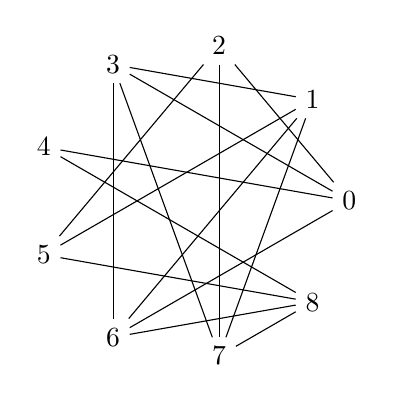
\begin{tikzpicture}
      \draw
        (0.0:2) node (0){0}
        (40.0:2) node (1){1}
        (80.0:2) node (2){2}
        (120.0:2) node (3){3}
        (160.0:2) node (4){4}
        (200.0:2) node (5){5}
        (240.0:2) node (6){6}
        (280.0:2) node (7){7}
        (320.0:2) node (8){8};
      \begin{scope}[-]
        \draw (0) to (2);
        \draw (0) to (3);
        \draw (0) to (4);
        \draw (0) to (6);
        \draw (1) to (3);
        \draw (1) to (5);
        \draw (1) to (6);
        \draw (1) to (7);
        \draw (2) to (5);
        \draw (2) to (7);
        \draw (3) to (6);
        \draw (3) to (7);
        \draw (4) to (8);
        \draw (5) to (8);
        \draw (6) to (8);
        \draw (7) to (8);
      \end{scope}
    \end{tikzpicture}
\end{figure}
\begin{itemize}
\item signature: 011101000101110001010001100001001011
\item g: Graph with 9 nodes and 16 edges
\item order: 9
\item size: 16
\item max degree: 4
\item degrees: 2,3,3,4,4,4,4,4,4
\item is tree: 0
\item is bipartite: 0
\item has bridge: 0
\item is chordal: 0
\item is complete: 0
\item min cycle basis weight: 29
\item min cycle basis size: 8
\item diameter: 3
\item radius: 2
\item is eulerian: 0
\item is planar: 0
\item number of faces: 9
\item is regular: 0
\item p3: 34
\item p4: 42
\item property hash: f98438c869b7e64c7660d9264512ff0676b3236bf1474578be5833f2d18b64ba
\end{itemize}
\newpage
\begin{figure}
  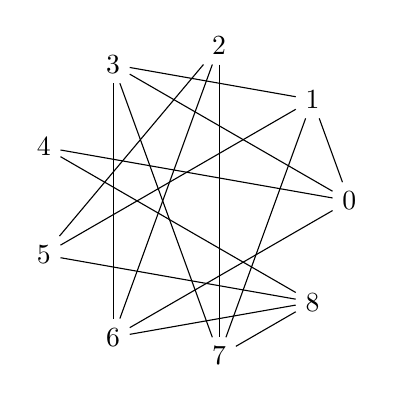
\begin{tikzpicture}
      \draw
        (0.0:2) node (0){0}
        (40.0:2) node (1){1}
        (80.0:2) node (2){2}
        (120.0:2) node (3){3}
        (160.0:2) node (4){4}
        (200.0:2) node (5){5}
        (240.0:2) node (6){6}
        (280.0:2) node (7){7}
        (320.0:2) node (8){8};
      \begin{scope}[-]
        \draw (0) to (1);
        \draw (0) to (3);
        \draw (0) to (4);
        \draw (0) to (6);
        \draw (1) to (3);
        \draw (1) to (5);
        \draw (1) to (7);
        \draw (2) to (5);
        \draw (2) to (6);
        \draw (2) to (7);
        \draw (3) to (6);
        \draw (3) to (7);
        \draw (4) to (8);
        \draw (5) to (8);
        \draw (6) to (8);
        \draw (7) to (8);
      \end{scope}
    \end{tikzpicture}
\end{figure}
\begin{itemize}
\item signature: 101101000101010001110001100001001011
\item g: Graph with 9 nodes and 16 edges
\item order: 9
\item size: 16
\item max degree: 4
\item degrees: 2,3,3,4,4,4,4,4,4
\item is tree: 0
\item is bipartite: 0
\item has bridge: 0
\item is chordal: 0
\item is complete: 0
\item min cycle basis weight: 29
\item min cycle basis size: 8
\item diameter: 3
\item radius: 2
\item is eulerian: 0
\item is planar: 0
\item number of faces: 9
\item is regular: 0
\item p3: 34
\item p4: 42
\item property hash: f98438c869b7e64c7660d9264512ff0676b3236bf1474578be5833f2d18b64ba
\end{itemize}
\newpage
\begin{figure}
  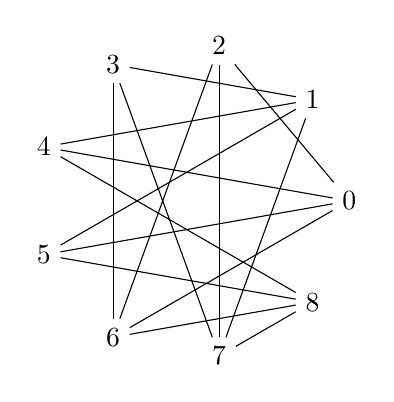
\begin{tikzpicture}
      \draw
        (0.0:2) node (0){0}
        (40.0:2) node (1){1}
        (80.0:2) node (2){2}
        (120.0:2) node (3){3}
        (160.0:2) node (4){4}
        (200.0:2) node (5){5}
        (240.0:2) node (6){6}
        (280.0:2) node (7){7}
        (320.0:2) node (8){8};
      \begin{scope}[-]
        \draw (0) to (2);
        \draw (0) to (4);
        \draw (0) to (5);
        \draw (0) to (6);
        \draw (1) to (3);
        \draw (1) to (4);
        \draw (1) to (5);
        \draw (1) to (7);
        \draw (2) to (6);
        \draw (2) to (7);
        \draw (3) to (6);
        \draw (3) to (7);
        \draw (4) to (8);
        \draw (5) to (8);
        \draw (6) to (8);
        \draw (7) to (8);
      \end{scope}
    \end{tikzpicture}
\end{figure}
\begin{itemize}
\item signature: 010111000111010000110001100001001011
\item g: Graph with 9 nodes and 16 edges
\item order: 9
\item size: 16
\item max degree: 4
\item degrees: 3,3,3,3,4,4,4,4,4
\item is tree: 0
\item is bipartite: 0
\item has bridge: 0
\item is chordal: 0
\item is complete: 0
\item min cycle basis weight: 30
\item min cycle basis size: 8
\item diameter: 2
\item radius: 2
\item is eulerian: 0
\item is planar: 0
\item number of faces: 9
\item is regular: 0
\item p3: 36
\item p4: 42
\item property hash: 65fd2abd97e29d97d09c02d99ddfe2ee7bc6b12c54177abb50a734b4ea4d9264
\end{itemize}
\newpage
\begin{figure}
  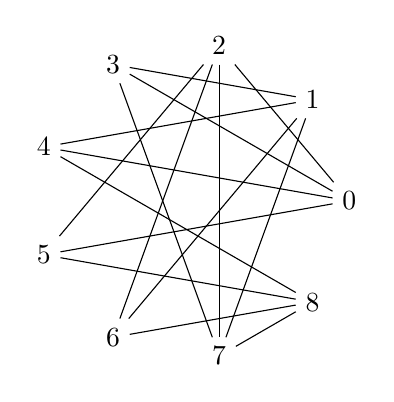
\begin{tikzpicture}
      \draw
        (0.0:2) node (0){0}
        (40.0:2) node (1){1}
        (80.0:2) node (2){2}
        (120.0:2) node (3){3}
        (160.0:2) node (4){4}
        (200.0:2) node (5){5}
        (240.0:2) node (6){6}
        (280.0:2) node (7){7}
        (320.0:2) node (8){8};
      \begin{scope}[-]
        \draw (0) to (2);
        \draw (0) to (3);
        \draw (0) to (4);
        \draw (0) to (5);
        \draw (1) to (3);
        \draw (1) to (4);
        \draw (1) to (6);
        \draw (1) to (7);
        \draw (2) to (5);
        \draw (2) to (6);
        \draw (2) to (7);
        \draw (3) to (7);
        \draw (4) to (8);
        \draw (5) to (8);
        \draw (6) to (8);
        \draw (7) to (8);
      \end{scope}
    \end{tikzpicture}
\end{figure}
\begin{itemize}
\item signature: 011110000110110001110000100001001011
\item g: Graph with 9 nodes and 16 edges
\item order: 9
\item size: 16
\item max degree: 4
\item degrees: 3,3,3,3,4,4,4,4,4
\item is tree: 0
\item is bipartite: 0
\item has bridge: 0
\item is chordal: 0
\item is complete: 0
\item min cycle basis weight: 30
\item min cycle basis size: 8
\item diameter: 3
\item radius: 2
\item is eulerian: 0
\item is planar: 0
\item number of faces: 9
\item is regular: 0
\item p3: 36
\item p4: 42
\item property hash: 4d4fdf8fe82e892c7d0a721bfd1bb438cbfcc5f8e1a8c8c16a216a6e054beb8a
\end{itemize}
\newpage
\begin{figure}
  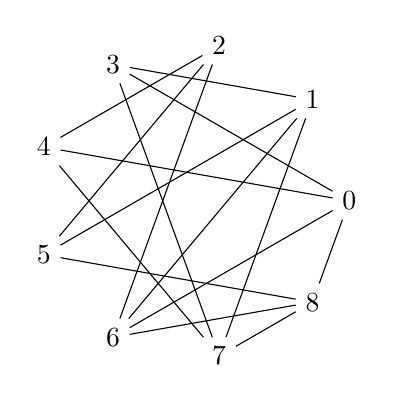
\begin{tikzpicture}
      \draw
        (0.0:2) node (0){0}
        (40.0:2) node (1){1}
        (80.0:2) node (2){2}
        (120.0:2) node (3){3}
        (160.0:2) node (4){4}
        (200.0:2) node (5){5}
        (240.0:2) node (6){6}
        (280.0:2) node (7){7}
        (320.0:2) node (8){8};
      \begin{scope}[-]
        \draw (0) to (3);
        \draw (0) to (4);
        \draw (0) to (6);
        \draw (0) to (8);
        \draw (1) to (3);
        \draw (1) to (5);
        \draw (1) to (6);
        \draw (1) to (7);
        \draw (2) to (4);
        \draw (2) to (5);
        \draw (2) to (6);
        \draw (3) to (7);
        \draw (4) to (7);
        \draw (5) to (8);
        \draw (6) to (8);
        \draw (7) to (8);
      \end{scope}
    \end{tikzpicture}
\end{figure}
\begin{itemize}
\item signature: 001101010101110011100000100010001011
\item g: Graph with 9 nodes and 16 edges
\item order: 9
\item size: 16
\item max degree: 4
\item degrees: 3,3,3,3,4,4,4,4,4
\item is tree: 0
\item is bipartite: 0
\item has bridge: 0
\item is chordal: 0
\item is complete: 0
\item min cycle basis weight: 30
\item min cycle basis size: 8
\item diameter: 3
\item radius: 2
\item is eulerian: 0
\item is planar: 0
\item number of faces: 9
\item is regular: 0
\item p3: 36
\item p4: 42
\item property hash: 4d4fdf8fe82e892c7d0a721bfd1bb438cbfcc5f8e1a8c8c16a216a6e054beb8a
\end{itemize}
\newpage
\begin{figure}
  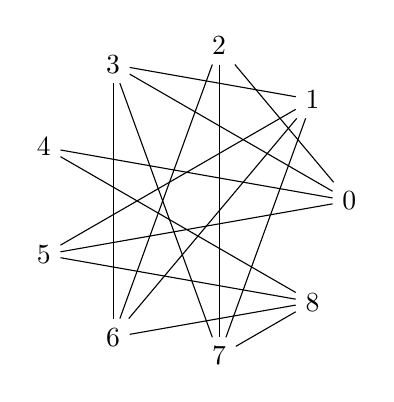
\begin{tikzpicture}
      \draw
        (0.0:2) node (0){0}
        (40.0:2) node (1){1}
        (80.0:2) node (2){2}
        (120.0:2) node (3){3}
        (160.0:2) node (4){4}
        (200.0:2) node (5){5}
        (240.0:2) node (6){6}
        (280.0:2) node (7){7}
        (320.0:2) node (8){8};
      \begin{scope}[-]
        \draw (0) to (2);
        \draw (0) to (3);
        \draw (0) to (4);
        \draw (0) to (5);
        \draw (1) to (3);
        \draw (1) to (5);
        \draw (1) to (6);
        \draw (1) to (7);
        \draw (2) to (6);
        \draw (2) to (7);
        \draw (3) to (6);
        \draw (3) to (7);
        \draw (4) to (8);
        \draw (5) to (8);
        \draw (6) to (8);
        \draw (7) to (8);
      \end{scope}
    \end{tikzpicture}
\end{figure}
\begin{itemize}
\item signature: 011110000101110000110001100001001011
\item g: Graph with 9 nodes and 16 edges
\item order: 9
\item size: 16
\item max degree: 4
\item degrees: 2,3,3,4,4,4,4,4,4
\item is tree: 0
\item is bipartite: 0
\item has bridge: 0
\item is chordal: 0
\item is complete: 0
\item min cycle basis weight: 30
\item min cycle basis size: 8
\item diameter: 3
\item radius: 2
\item is eulerian: 0
\item is planar: 0
\item number of faces: 9
\item is regular: 0
\item p3: 37
\item p4: 42
\item property hash: 733f0467b56b29a6701d6d58cd7d8f190fb726077791d67056b2d320eb3046e9
\end{itemize}
\newpage
\begin{figure}
  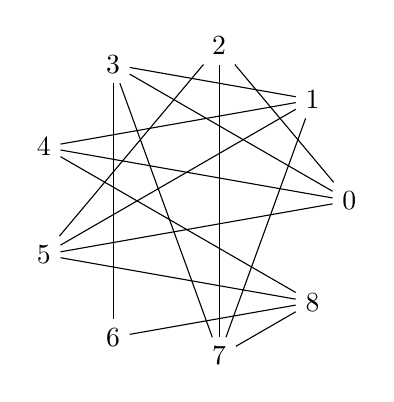
\begin{tikzpicture}
      \draw
        (0.0:2) node (0){0}
        (40.0:2) node (1){1}
        (80.0:2) node (2){2}
        (120.0:2) node (3){3}
        (160.0:2) node (4){4}
        (200.0:2) node (5){5}
        (240.0:2) node (6){6}
        (280.0:2) node (7){7}
        (320.0:2) node (8){8};
      \begin{scope}[-]
        \draw (0) to (2);
        \draw (0) to (3);
        \draw (0) to (4);
        \draw (0) to (5);
        \draw (1) to (3);
        \draw (1) to (4);
        \draw (1) to (5);
        \draw (1) to (7);
        \draw (2) to (5);
        \draw (2) to (7);
        \draw (3) to (6);
        \draw (3) to (7);
        \draw (4) to (8);
        \draw (5) to (8);
        \draw (6) to (8);
        \draw (7) to (8);
      \end{scope}
    \end{tikzpicture}
\end{figure}
\begin{itemize}
\item signature: 011110000111010001010001100001001011
\item g: Graph with 9 nodes and 16 edges
\item order: 9
\item size: 16
\item max degree: 4
\item degrees: 2,3,3,4,4,4,4,4,4
\item is tree: 0
\item is bipartite: 0
\item has bridge: 0
\item is chordal: 0
\item is complete: 0
\item min cycle basis weight: 30
\item min cycle basis size: 8
\item diameter: 3
\item radius: 2
\item is eulerian: 0
\item is planar: 0
\item number of faces: 9
\item is regular: 0
\item p3: 37
\item p4: 42
\item property hash: 733f0467b56b29a6701d6d58cd7d8f190fb726077791d67056b2d320eb3046e9
\end{itemize}
\newpage
\begin{figure}
  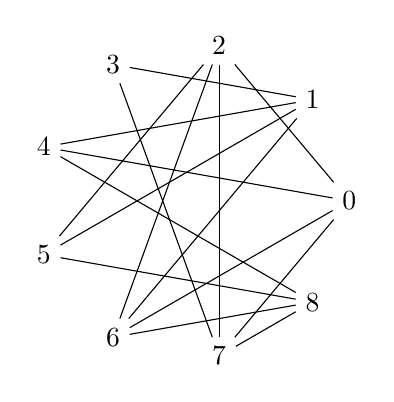
\begin{tikzpicture}
      \draw
        (0.0:2) node (0){0}
        (40.0:2) node (1){1}
        (80.0:2) node (2){2}
        (120.0:2) node (3){3}
        (160.0:2) node (4){4}
        (200.0:2) node (5){5}
        (240.0:2) node (6){6}
        (280.0:2) node (7){7}
        (320.0:2) node (8){8};
      \begin{scope}[-]
        \draw (0) to (2);
        \draw (0) to (4);
        \draw (0) to (6);
        \draw (0) to (7);
        \draw (1) to (3);
        \draw (1) to (4);
        \draw (1) to (5);
        \draw (1) to (6);
        \draw (2) to (5);
        \draw (2) to (6);
        \draw (2) to (7);
        \draw (3) to (7);
        \draw (4) to (8);
        \draw (5) to (8);
        \draw (6) to (8);
        \draw (7) to (8);
      \end{scope}
    \end{tikzpicture}
\end{figure}
\begin{itemize}
\item signature: 010101100111100001110000100001001011
\item g: Graph with 9 nodes and 16 edges
\item order: 9
\item size: 16
\item max degree: 4
\item degrees: 2,3,3,4,4,4,4,4,4
\item is tree: 0
\item is bipartite: 0
\item has bridge: 0
\item is chordal: 0
\item is complete: 0
\item min cycle basis weight: 31
\item min cycle basis size: 8
\item diameter: 2
\item radius: 2
\item is eulerian: 0
\item is planar: 0
\item number of faces: 9
\item is regular: 0
\item p3: 37
\item p4: 42
\item property hash: 717769325ce0490c76bd161f9a529b2e40f64ed0de6b0179e3f0131d2d006ea7
\end{itemize}
\newpage
\begin{figure}
  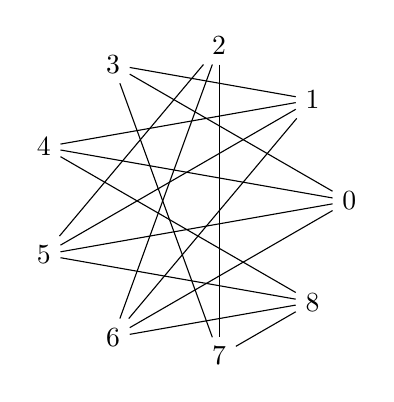
\begin{tikzpicture}
      \draw
        (0.0:2) node (0){0}
        (40.0:2) node (1){1}
        (80.0:2) node (2){2}
        (120.0:2) node (3){3}
        (160.0:2) node (4){4}
        (200.0:2) node (5){5}
        (240.0:2) node (6){6}
        (280.0:2) node (7){7}
        (320.0:2) node (8){8};
      \begin{scope}[-]
        \draw (0) to (3);
        \draw (0) to (4);
        \draw (0) to (5);
        \draw (0) to (6);
        \draw (1) to (3);
        \draw (1) to (4);
        \draw (1) to (5);
        \draw (1) to (6);
        \draw (2) to (5);
        \draw (2) to (6);
        \draw (2) to (7);
        \draw (3) to (7);
        \draw (4) to (8);
        \draw (5) to (8);
        \draw (6) to (8);
        \draw (7) to (8);
      \end{scope}
    \end{tikzpicture}
\end{figure}
\begin{itemize}
\item signature: 001111000111100001110000100001001011
\item g: Graph with 9 nodes and 16 edges
\item order: 9
\item size: 16
\item max degree: 4
\item degrees: 3,3,3,3,4,4,4,4,4
\item is tree: 0
\item is bipartite: 0
\item has bridge: 0
\item is chordal: 0
\item is complete: 0
\item min cycle basis weight: 33
\item min cycle basis size: 8
\item diameter: 3
\item radius: 2
\item is eulerian: 0
\item is planar: 0
\item number of faces: 9
\item is regular: 0
\item p3: 42
\item p4: 42
\item property hash: 74ecca7a986cf96bbf915926a848218d501cfb3f495e79a55f1bb0a243265c49
\end{itemize}
\newpage
\begin{figure}
  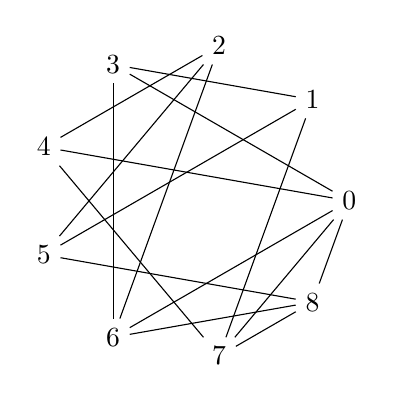
\begin{tikzpicture}
      \draw
        (0.0:2) node (0){0}
        (40.0:2) node (1){1}
        (80.0:2) node (2){2}
        (120.0:2) node (3){3}
        (160.0:2) node (4){4}
        (200.0:2) node (5){5}
        (240.0:2) node (6){6}
        (280.0:2) node (7){7}
        (320.0:2) node (8){8};
      \begin{scope}[-]
        \draw (0) to (3);
        \draw (0) to (4);
        \draw (0) to (6);
        \draw (0) to (7);
        \draw (0) to (8);
        \draw (1) to (3);
        \draw (1) to (5);
        \draw (1) to (7);
        \draw (2) to (4);
        \draw (2) to (5);
        \draw (2) to (6);
        \draw (3) to (6);
        \draw (4) to (7);
        \draw (5) to (8);
        \draw (6) to (8);
        \draw (7) to (8);
      \end{scope}
    \end{tikzpicture}
\end{figure}
\begin{itemize}
\item signature: 001101110101010011100001000010001011
\item g: Graph with 9 nodes and 16 edges
\item order: 9
\item size: 16
\item max degree: 5
\item degrees: 3,3,3,3,3,4,4,4,5
\item is tree: 0
\item is bipartite: 0
\item has bridge: 0
\item is chordal: 0
\item is complete: 0
\item min cycle basis weight: 28
\item min cycle basis size: 8
\item diameter: 2
\item radius: 2
\item is eulerian: 0
\item is planar: 0
\item number of faces: 9
\item is regular: 0
\item p3: 31
\item p4: 42
\item property hash: a3e4551bfa4796681fc499ed9144adb8f5131e396f012d612f01c1be7dc5c7ed
\end{itemize}
\newpage
\begin{figure}
  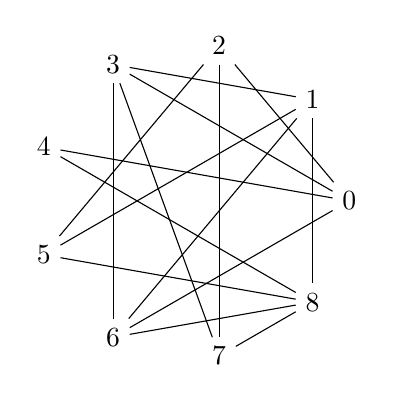
\begin{tikzpicture}
      \draw
        (0.0:2) node (0){0}
        (40.0:2) node (1){1}
        (80.0:2) node (2){2}
        (120.0:2) node (3){3}
        (160.0:2) node (4){4}
        (200.0:2) node (5){5}
        (240.0:2) node (6){6}
        (280.0:2) node (7){7}
        (320.0:2) node (8){8};
      \begin{scope}[-]
        \draw (0) to (2);
        \draw (0) to (3);
        \draw (0) to (4);
        \draw (0) to (6);
        \draw (1) to (3);
        \draw (1) to (5);
        \draw (1) to (6);
        \draw (1) to (8);
        \draw (2) to (5);
        \draw (2) to (7);
        \draw (3) to (6);
        \draw (3) to (7);
        \draw (4) to (8);
        \draw (5) to (8);
        \draw (6) to (8);
        \draw (7) to (8);
      \end{scope}
    \end{tikzpicture}
\end{figure}
\begin{itemize}
\item signature: 011101000101101001010001100001001011
\item g: Graph with 9 nodes and 16 edges
\item order: 9
\item size: 16
\item max degree: 5
\item degrees: 2,3,3,3,4,4,4,4,5
\item is tree: 0
\item is bipartite: 0
\item has bridge: 0
\item is chordal: 0
\item is complete: 0
\item min cycle basis weight: 28
\item min cycle basis size: 8
\item diameter: 2
\item radius: 2
\item is eulerian: 0
\item is planar: 0
\item number of faces: 9
\item is regular: 0
\item p3: 32
\item p4: 42
\item property hash: 65e4aa27f213ed33a0e522a3d5c4aaa1af58ab538fd2b5631484655ecca88d71
\end{itemize}
\newpage
\begin{figure}
  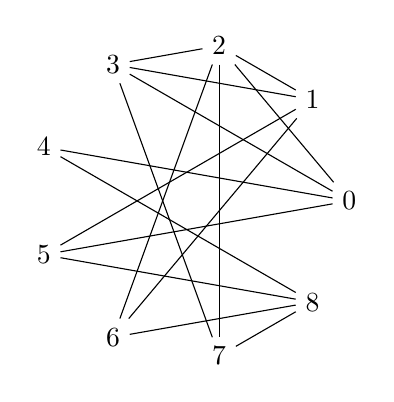
\begin{tikzpicture}
      \draw
        (0.0:2) node (0){0}
        (40.0:2) node (1){1}
        (80.0:2) node (2){2}
        (120.0:2) node (3){3}
        (160.0:2) node (4){4}
        (200.0:2) node (5){5}
        (240.0:2) node (6){6}
        (280.0:2) node (7){7}
        (320.0:2) node (8){8};
      \begin{scope}[-]
        \draw (0) to (2);
        \draw (0) to (3);
        \draw (0) to (4);
        \draw (0) to (5);
        \draw (1) to (2);
        \draw (1) to (3);
        \draw (1) to (5);
        \draw (1) to (6);
        \draw (2) to (3);
        \draw (2) to (6);
        \draw (2) to (7);
        \draw (3) to (7);
        \draw (4) to (8);
        \draw (5) to (8);
        \draw (6) to (8);
        \draw (7) to (8);
      \end{scope}
    \end{tikzpicture}
\end{figure}
\begin{itemize}
\item signature: 011110001101100100110000100001001011
\item g: Graph with 9 nodes and 16 edges
\item order: 9
\item size: 16
\item max degree: 5
\item degrees: 2,3,3,3,4,4,4,4,5
\item is tree: 0
\item is bipartite: 0
\item has bridge: 0
\item is chordal: 0
\item is complete: 0
\item min cycle basis weight: 28
\item min cycle basis size: 8
\item diameter: 3
\item radius: 2
\item is eulerian: 0
\item is planar: 0
\item number of faces: 9
\item is regular: 0
\item p3: 32
\item p4: 42
\item property hash: 2d88a11d63b7dd859fb82e5edffd59e7301da5ef6185bda3b08b61ba1be9f2ae
\end{itemize}
\newpage
\begin{figure}
  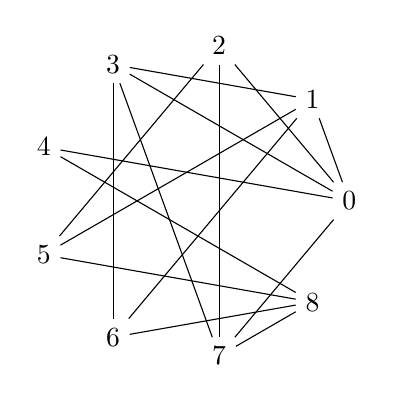
\begin{tikzpicture}
      \draw
        (0.0:2) node (0){0}
        (40.0:2) node (1){1}
        (80.0:2) node (2){2}
        (120.0:2) node (3){3}
        (160.0:2) node (4){4}
        (200.0:2) node (5){5}
        (240.0:2) node (6){6}
        (280.0:2) node (7){7}
        (320.0:2) node (8){8};
      \begin{scope}[-]
        \draw (0) to (1);
        \draw (0) to (2);
        \draw (0) to (3);
        \draw (0) to (4);
        \draw (0) to (7);
        \draw (1) to (3);
        \draw (1) to (5);
        \draw (1) to (6);
        \draw (2) to (5);
        \draw (2) to (7);
        \draw (3) to (6);
        \draw (3) to (7);
        \draw (4) to (8);
        \draw (5) to (8);
        \draw (6) to (8);
        \draw (7) to (8);
      \end{scope}
    \end{tikzpicture}
\end{figure}
\begin{itemize}
\item signature: 111100100101100001010001100001001011
\item g: Graph with 9 nodes and 16 edges
\item order: 9
\item size: 16
\item max degree: 5
\item degrees: 2,3,3,3,4,4,4,4,5
\item is tree: 0
\item is bipartite: 0
\item has bridge: 0
\item is chordal: 0
\item is complete: 0
\item min cycle basis weight: 28
\item min cycle basis size: 8
\item diameter: 3
\item radius: 2
\item is eulerian: 0
\item is planar: 0
\item number of faces: 9
\item is regular: 0
\item p3: 32
\item p4: 42
\item property hash: 2d88a11d63b7dd859fb82e5edffd59e7301da5ef6185bda3b08b61ba1be9f2ae
\end{itemize}
\newpage
\begin{figure}
  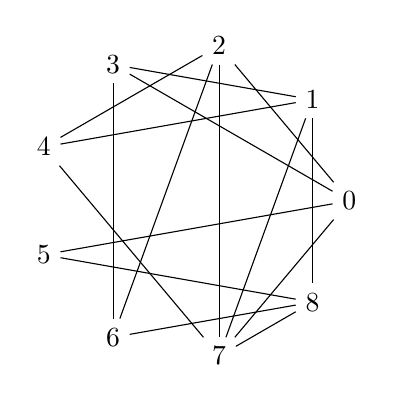
\begin{tikzpicture}
      \draw
        (0.0:2) node (0){0}
        (40.0:2) node (1){1}
        (80.0:2) node (2){2}
        (120.0:2) node (3){3}
        (160.0:2) node (4){4}
        (200.0:2) node (5){5}
        (240.0:2) node (6){6}
        (280.0:2) node (7){7}
        (320.0:2) node (8){8};
      \begin{scope}[-]
        \draw (0) to (2);
        \draw (0) to (3);
        \draw (0) to (5);
        \draw (0) to (7);
        \draw (1) to (3);
        \draw (1) to (4);
        \draw (1) to (7);
        \draw (1) to (8);
        \draw (2) to (4);
        \draw (2) to (6);
        \draw (2) to (7);
        \draw (3) to (6);
        \draw (4) to (7);
        \draw (5) to (8);
        \draw (6) to (8);
        \draw (7) to (8);
      \end{scope}
    \end{tikzpicture}
\end{figure}
\begin{itemize}
\item signature: 011010100110011010110001000010001011
\item g: Graph with 9 nodes and 16 edges
\item order: 9
\item size: 16
\item max degree: 5
\item degrees: 2,3,3,3,4,4,4,4,5
\item is tree: 0
\item is bipartite: 0
\item has bridge: 0
\item is chordal: 0
\item is complete: 0
\item min cycle basis weight: 28
\item min cycle basis size: 8
\item diameter: 3
\item radius: 2
\item is eulerian: 0
\item is planar: 0
\item number of faces: 9
\item is regular: 0
\item p3: 32
\item p4: 42
\item property hash: 2d88a11d63b7dd859fb82e5edffd59e7301da5ef6185bda3b08b61ba1be9f2ae
\end{itemize}
\newpage
\begin{figure}
  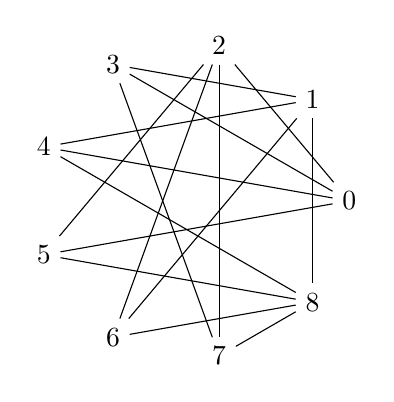
\begin{tikzpicture}
      \draw
        (0.0:2) node (0){0}
        (40.0:2) node (1){1}
        (80.0:2) node (2){2}
        (120.0:2) node (3){3}
        (160.0:2) node (4){4}
        (200.0:2) node (5){5}
        (240.0:2) node (6){6}
        (280.0:2) node (7){7}
        (320.0:2) node (8){8};
      \begin{scope}[-]
        \draw (0) to (2);
        \draw (0) to (3);
        \draw (0) to (4);
        \draw (0) to (5);
        \draw (1) to (3);
        \draw (1) to (4);
        \draw (1) to (6);
        \draw (1) to (8);
        \draw (2) to (5);
        \draw (2) to (6);
        \draw (2) to (7);
        \draw (3) to (7);
        \draw (4) to (8);
        \draw (5) to (8);
        \draw (6) to (8);
        \draw (7) to (8);
      \end{scope}
    \end{tikzpicture}
\end{figure}
\begin{itemize}
\item signature: 011110000110101001110000100001001011
\item g: Graph with 9 nodes and 16 edges
\item order: 9
\item size: 16
\item max degree: 5
\item degrees: 3,3,3,3,3,4,4,4,5
\item is tree: 0
\item is bipartite: 0
\item has bridge: 0
\item is chordal: 0
\item is complete: 0
\item min cycle basis weight: 29
\item min cycle basis size: 8
\item diameter: 2
\item radius: 2
\item is eulerian: 0
\item is planar: 0
\item number of faces: 9
\item is regular: 0
\item p3: 34
\item p4: 42
\item property hash: 17b414b23fe6caa4a3ae1c6ccbe5f775144046b47c732117310466121a0f5878
\end{itemize}
\newpage
\begin{figure}
  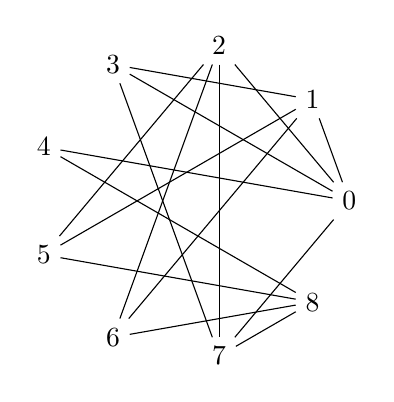
\begin{tikzpicture}
      \draw
        (0.0:2) node (0){0}
        (40.0:2) node (1){1}
        (80.0:2) node (2){2}
        (120.0:2) node (3){3}
        (160.0:2) node (4){4}
        (200.0:2) node (5){5}
        (240.0:2) node (6){6}
        (280.0:2) node (7){7}
        (320.0:2) node (8){8};
      \begin{scope}[-]
        \draw (0) to (1);
        \draw (0) to (2);
        \draw (0) to (3);
        \draw (0) to (4);
        \draw (0) to (7);
        \draw (1) to (3);
        \draw (1) to (5);
        \draw (1) to (6);
        \draw (2) to (5);
        \draw (2) to (6);
        \draw (2) to (7);
        \draw (3) to (7);
        \draw (4) to (8);
        \draw (5) to (8);
        \draw (6) to (8);
        \draw (7) to (8);
      \end{scope}
    \end{tikzpicture}
\end{figure}
\begin{itemize}
\item signature: 111100100101100001110000100001001011
\item g: Graph with 9 nodes and 16 edges
\item order: 9
\item size: 16
\item max degree: 5
\item degrees: 2,3,3,3,4,4,4,4,5
\item is tree: 0
\item is bipartite: 0
\item has bridge: 0
\item is chordal: 0
\item is complete: 0
\item min cycle basis weight: 29
\item min cycle basis size: 8
\item diameter: 2
\item radius: 2
\item is eulerian: 0
\item is planar: 0
\item number of faces: 9
\item is regular: 0
\item p3: 35
\item p4: 42
\item property hash: 61ce5d84408b3c2ddb5f99c6499d08767a62df59a5b0734fba599b69c6418495
\end{itemize}
\newpage
\begin{figure}
  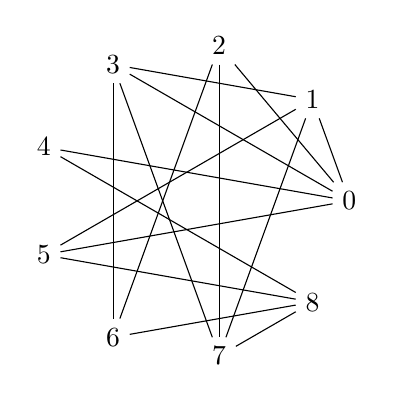
\begin{tikzpicture}
      \draw
        (0.0:2) node (0){0}
        (40.0:2) node (1){1}
        (80.0:2) node (2){2}
        (120.0:2) node (3){3}
        (160.0:2) node (4){4}
        (200.0:2) node (5){5}
        (240.0:2) node (6){6}
        (280.0:2) node (7){7}
        (320.0:2) node (8){8};
      \begin{scope}[-]
        \draw (0) to (1);
        \draw (0) to (2);
        \draw (0) to (3);
        \draw (0) to (4);
        \draw (0) to (5);
        \draw (1) to (3);
        \draw (1) to (5);
        \draw (1) to (7);
        \draw (2) to (6);
        \draw (2) to (7);
        \draw (3) to (6);
        \draw (3) to (7);
        \draw (4) to (8);
        \draw (5) to (8);
        \draw (6) to (8);
        \draw (7) to (8);
      \end{scope}
    \end{tikzpicture}
\end{figure}
\begin{itemize}
\item signature: 111110000101010000110001100001001011
\item g: Graph with 9 nodes and 16 edges
\item order: 9
\item size: 16
\item max degree: 5
\item degrees: 2,3,3,3,4,4,4,4,5
\item is tree: 0
\item is bipartite: 0
\item has bridge: 0
\item is chordal: 0
\item is complete: 0
\item min cycle basis weight: 29
\item min cycle basis size: 8
\item diameter: 2
\item radius: 2
\item is eulerian: 0
\item is planar: 0
\item number of faces: 9
\item is regular: 0
\item p3: 35
\item p4: 42
\item property hash: 61ce5d84408b3c2ddb5f99c6499d08767a62df59a5b0734fba599b69c6418495
\end{itemize}
\newpage
\begin{figure}
  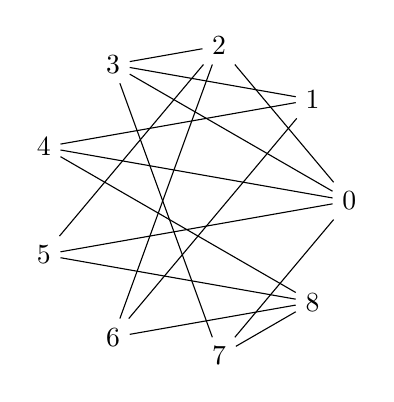
\begin{tikzpicture}
      \draw
        (0.0:2) node (0){0}
        (40.0:2) node (1){1}
        (80.0:2) node (2){2}
        (120.0:2) node (3){3}
        (160.0:2) node (4){4}
        (200.0:2) node (5){5}
        (240.0:2) node (6){6}
        (280.0:2) node (7){7}
        (320.0:2) node (8){8};
      \begin{scope}[-]
        \draw (0) to (2);
        \draw (0) to (3);
        \draw (0) to (4);
        \draw (0) to (5);
        \draw (0) to (7);
        \draw (1) to (3);
        \draw (1) to (4);
        \draw (1) to (6);
        \draw (2) to (3);
        \draw (2) to (5);
        \draw (2) to (6);
        \draw (3) to (7);
        \draw (4) to (8);
        \draw (5) to (8);
        \draw (6) to (8);
        \draw (7) to (8);
      \end{scope}
    \end{tikzpicture}
\end{figure}
\begin{itemize}
\item signature: 011110100110100101100000100001001011
\item g: Graph with 9 nodes and 16 edges
\item order: 9
\item size: 16
\item max degree: 5
\item degrees: 3,3,3,3,3,4,4,4,5
\item is tree: 0
\item is bipartite: 0
\item has bridge: 0
\item is chordal: 0
\item is complete: 0
\item min cycle basis weight: 29
\item min cycle basis size: 8
\item diameter: 3
\item radius: 2
\item is eulerian: 0
\item is planar: 0
\item number of faces: 9
\item is regular: 0
\item p3: 34
\item p4: 42
\item property hash: 4a11ca195ca06e78f7c77a9e31eee7f50801469e80ff0e90017e40a6e478a4fb
\end{itemize}
\newpage
\begin{figure}
  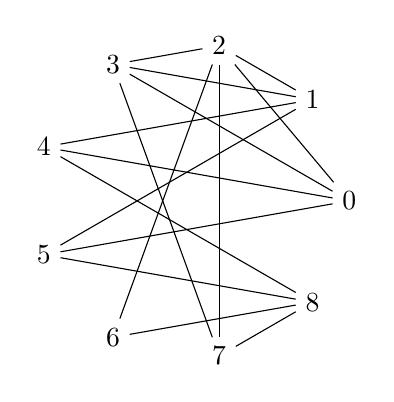
\begin{tikzpicture}
      \draw
        (0.0:2) node (0){0}
        (40.0:2) node (1){1}
        (80.0:2) node (2){2}
        (120.0:2) node (3){3}
        (160.0:2) node (4){4}
        (200.0:2) node (5){5}
        (240.0:2) node (6){6}
        (280.0:2) node (7){7}
        (320.0:2) node (8){8};
      \begin{scope}[-]
        \draw (0) to (2);
        \draw (0) to (3);
        \draw (0) to (4);
        \draw (0) to (5);
        \draw (1) to (2);
        \draw (1) to (3);
        \draw (1) to (4);
        \draw (1) to (5);
        \draw (2) to (3);
        \draw (2) to (6);
        \draw (2) to (7);
        \draw (3) to (7);
        \draw (4) to (8);
        \draw (5) to (8);
        \draw (6) to (8);
        \draw (7) to (8);
      \end{scope}
    \end{tikzpicture}
\end{figure}
\begin{itemize}
\item signature: 011110001111000100110000100001001011
\item g: Graph with 9 nodes and 16 edges
\item order: 9
\item size: 16
\item max degree: 5
\item degrees: 2,3,3,3,4,4,4,4,5
\item is tree: 0
\item is bipartite: 0
\item has bridge: 0
\item is chordal: 0
\item is complete: 0
\item min cycle basis weight: 30
\item min cycle basis size: 8
\item diameter: 2
\item radius: 2
\item is eulerian: 0
\item is planar: 0
\item number of faces: 9
\item is regular: 0
\item p3: 35
\item p4: 42
\item property hash: 1826d3399058342021ae226f714349352f29beb553d5d328f374374d5f61049c
\end{itemize}
\newpage
\begin{figure}
  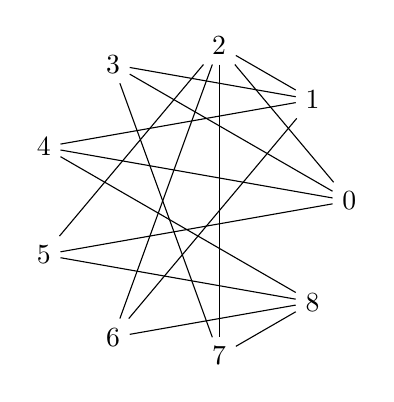
\begin{tikzpicture}
      \draw
        (0.0:2) node (0){0}
        (40.0:2) node (1){1}
        (80.0:2) node (2){2}
        (120.0:2) node (3){3}
        (160.0:2) node (4){4}
        (200.0:2) node (5){5}
        (240.0:2) node (6){6}
        (280.0:2) node (7){7}
        (320.0:2) node (8){8};
      \begin{scope}[-]
        \draw (0) to (2);
        \draw (0) to (3);
        \draw (0) to (4);
        \draw (0) to (5);
        \draw (1) to (2);
        \draw (1) to (3);
        \draw (1) to (4);
        \draw (1) to (6);
        \draw (2) to (5);
        \draw (2) to (6);
        \draw (2) to (7);
        \draw (3) to (7);
        \draw (4) to (8);
        \draw (5) to (8);
        \draw (6) to (8);
        \draw (7) to (8);
      \end{scope}
    \end{tikzpicture}
\end{figure}
\begin{itemize}
\item signature: 011110001110100001110000100001001011
\item g: Graph with 9 nodes and 16 edges
\item order: 9
\item size: 16
\item max degree: 5
\item degrees: 3,3,3,3,3,4,4,4,5
\item is tree: 0
\item is bipartite: 0
\item has bridge: 0
\item is chordal: 0
\item is complete: 0
\item min cycle basis weight: 30
\item min cycle basis size: 8
\item diameter: 2
\item radius: 2
\item is eulerian: 0
\item is planar: 0
\item number of faces: 9
\item is regular: 0
\item p3: 37
\item p4: 42
\item property hash: e18c2e06a8ec93672c7325b35a16cbed7e059297da4442edb0cd1d7bb4ece313
\end{itemize}
\newpage
\begin{figure}
  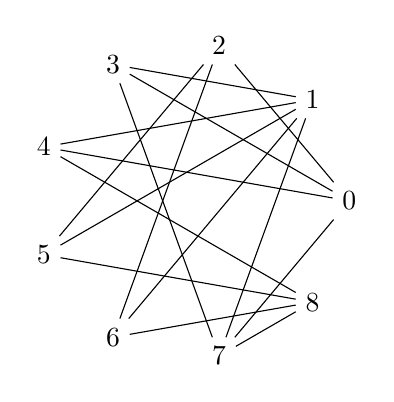
\begin{tikzpicture}
      \draw
        (0.0:2) node (0){0}
        (40.0:2) node (1){1}
        (80.0:2) node (2){2}
        (120.0:2) node (3){3}
        (160.0:2) node (4){4}
        (200.0:2) node (5){5}
        (240.0:2) node (6){6}
        (280.0:2) node (7){7}
        (320.0:2) node (8){8};
      \begin{scope}[-]
        \draw (0) to (2);
        \draw (0) to (3);
        \draw (0) to (4);
        \draw (0) to (7);
        \draw (1) to (3);
        \draw (1) to (4);
        \draw (1) to (5);
        \draw (1) to (6);
        \draw (1) to (7);
        \draw (2) to (5);
        \draw (2) to (6);
        \draw (3) to (7);
        \draw (4) to (8);
        \draw (5) to (8);
        \draw (6) to (8);
        \draw (7) to (8);
      \end{scope}
    \end{tikzpicture}
\end{figure}
\begin{itemize}
\item signature: 011100100111110001100000100001001011
\item g: Graph with 9 nodes and 16 edges
\item order: 9
\item size: 16
\item max degree: 5
\item degrees: 3,3,3,3,3,4,4,4,5
\item is tree: 0
\item is bipartite: 0
\item has bridge: 0
\item is chordal: 0
\item is complete: 0
\item min cycle basis weight: 31
\item min cycle basis size: 8
\item diameter: 2
\item radius: 2
\item is eulerian: 0
\item is planar: 0
\item number of faces: 9
\item is regular: 0
\item p3: 37
\item p4: 42
\item property hash: 82ba241d7f5bd0a9e022cfdb333f95da79726573800d5edb4b83ac847eab533d
\end{itemize}
\newpage
\begin{figure}
  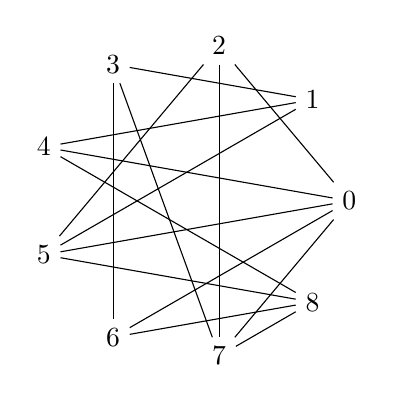
\begin{tikzpicture}
      \draw
        (0.0:2) node (0){0}
        (40.0:2) node (1){1}
        (80.0:2) node (2){2}
        (120.0:2) node (3){3}
        (160.0:2) node (4){4}
        (200.0:2) node (5){5}
        (240.0:2) node (6){6}
        (280.0:2) node (7){7}
        (320.0:2) node (8){8};
      \begin{scope}[-]
        \draw (0) to (2);
        \draw (0) to (4);
        \draw (0) to (5);
        \draw (0) to (6);
        \draw (0) to (7);
        \draw (1) to (3);
        \draw (1) to (4);
        \draw (1) to (5);
        \draw (2) to (5);
        \draw (2) to (7);
        \draw (3) to (6);
        \draw (3) to (7);
        \draw (4) to (8);
        \draw (5) to (8);
        \draw (6) to (8);
        \draw (7) to (8);
      \end{scope}
    \end{tikzpicture}
\end{figure}
\begin{itemize}
\item signature: 010111100111000001010001100001001011
\item g: Graph with 9 nodes and 16 edges
\item order: 9
\item size: 16
\item max degree: 5
\item degrees: 3,3,3,3,3,4,4,4,5
\item is tree: 0
\item is bipartite: 0
\item has bridge: 0
\item is chordal: 0
\item is complete: 0
\item min cycle basis weight: 31
\item min cycle basis size: 8
\item diameter: 2
\item radius: 2
\item is eulerian: 0
\item is planar: 0
\item number of faces: 9
\item is regular: 0
\item p3: 37
\item p4: 42
\item property hash: 82ba241d7f5bd0a9e022cfdb333f95da79726573800d5edb4b83ac847eab533d
\end{itemize}
\newpage
\begin{figure}
  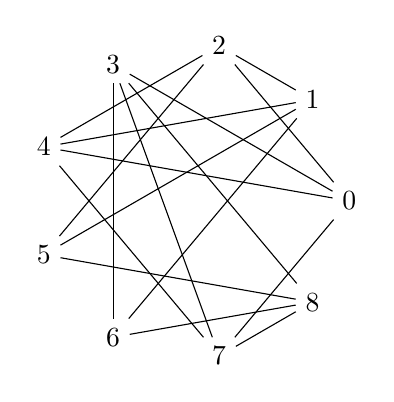
\begin{tikzpicture}
      \draw
        (0.0:2) node (0){0}
        (40.0:2) node (1){1}
        (80.0:2) node (2){2}
        (120.0:2) node (3){3}
        (160.0:2) node (4){4}
        (200.0:2) node (5){5}
        (240.0:2) node (6){6}
        (280.0:2) node (7){7}
        (320.0:2) node (8){8};
      \begin{scope}[-]
        \draw (0) to (2);
        \draw (0) to (3);
        \draw (0) to (4);
        \draw (0) to (7);
        \draw (1) to (2);
        \draw (1) to (4);
        \draw (1) to (5);
        \draw (1) to (6);
        \draw (2) to (4);
        \draw (2) to (5);
        \draw (3) to (6);
        \draw (3) to (7);
        \draw (3) to (8);
        \draw (4) to (7);
        \draw (5) to (8);
        \draw (6) to (8);
        \draw (7) to (8);
      \end{scope}
    \end{tikzpicture}
\end{figure}
\begin{itemize}
\item signature: 011100101011100011000001110010001011
\item g: Graph with 9 nodes and 17 edges
\item order: 9
\item size: 17
\item max degree: 4
\item degrees: 3,3,4,4,4,4,4,4,4
\item is tree: 0
\item is bipartite: 0
\item has bridge: 0
\item is chordal: 0
\item is complete: 0
\item min cycle basis weight: 30
\item min cycle basis size: 9
\item diameter: 2
\item radius: 2
\item is eulerian: 0
\item is planar: 0
\item number of faces: 10
\item is regular: 0
\item p3: 27
\item p4: 42
\item property hash: 587ec57b1e1841ffc3d9eb0fcfbe2a6d08cd332afe8d4ff07b410ab88c12a0b1
\end{itemize}
\newpage
\begin{figure}
  \begin{tikzpicture}
      \draw
        (0.0:2) node (0){0}
        (40.0:2) node (1){1}
        (80.0:2) node (2){2}
        (120.0:2) node (3){3}
        (160.0:2) node (4){4}
        (200.0:2) node (5){5}
        (240.0:2) node (6){6}
        (280.0:2) node (7){7}
        (320.0:2) node (8){8};
      \begin{scope}[-]
        \draw (0) to (2);
        \draw (0) to (3);
        \draw (0) to (5);
        \draw (0) to (6);
        \draw (1) to (3);
        \draw (1) to (4);
        \draw (1) to (5);
        \draw (1) to (7);
        \draw (2) to (4);
        \draw (2) to (6);
        \draw (2) to (7);
        \draw (3) to (6);
        \draw (3) to (8);
        \draw (4) to (7);
        \draw (5) to (8);
        \draw (6) to (8);
        \draw (7) to (8);
      \end{scope}
    \end{tikzpicture}
\end{figure}
\begin{itemize}
\item signature: 011011000111010010110001010010001011
\item g: Graph with 9 nodes and 17 edges
\item order: 9
\item size: 17
\item max degree: 4
\item degrees: 3,3,4,4,4,4,4,4,4
\item is tree: 0
\item is bipartite: 0
\item has bridge: 0
\item is chordal: 0
\item is complete: 0
\item min cycle basis weight: 31
\item min cycle basis size: 9
\item diameter: 2
\item radius: 2
\item is eulerian: 0
\item is planar: 0
\item number of faces: 10
\item is regular: 0
\item p3: 33
\item p4: 42
\item property hash: 3ab1761af72c65d77e8ce2767d8746fbc7ab3ba175792f48eacb4198cc00d91c
\end{itemize}
\newpage
\begin{figure}
  \begin{tikzpicture}
      \draw
        (0.0:2) node (0){0}
        (40.0:2) node (1){1}
        (80.0:2) node (2){2}
        (120.0:2) node (3){3}
        (160.0:2) node (4){4}
        (200.0:2) node (5){5}
        (240.0:2) node (6){6}
        (280.0:2) node (7){7}
        (320.0:2) node (8){8};
      \begin{scope}[-]
        \draw (0) to (2);
        \draw (0) to (3);
        \draw (0) to (4);
        \draw (0) to (5);
        \draw (1) to (3);
        \draw (1) to (4);
        \draw (1) to (5);
        \draw (1) to (7);
        \draw (2) to (5);
        \draw (2) to (6);
        \draw (2) to (8);
        \draw (3) to (6);
        \draw (3) to (7);
        \draw (4) to (7);
        \draw (5) to (8);
        \draw (6) to (8);
        \draw (7) to (8);
      \end{scope}
    \end{tikzpicture}
\end{figure}
\begin{itemize}
\item signature: 011110000111010001101001100010001011
\item g: Graph with 9 nodes and 17 edges
\item order: 9
\item size: 17
\item max degree: 4
\item degrees: 3,3,4,4,4,4,4,4,4
\item is tree: 0
\item is bipartite: 0
\item has bridge: 0
\item is chordal: 0
\item is complete: 0
\item min cycle basis weight: 31
\item min cycle basis size: 9
\item diameter: 3
\item radius: 2
\item is eulerian: 0
\item is planar: 0
\item number of faces: 10
\item is regular: 0
\item p3: 33
\item p4: 42
\item property hash: bd172241c8e0075ebc44c0f0cf9fa31558636213a4ccb12ac03091f7cc1124de
\end{itemize}
\newpage
\begin{figure}
  \begin{tikzpicture}
      \draw
        (0.0:2) node (0){0}
        (40.0:2) node (1){1}
        (80.0:2) node (2){2}
        (120.0:2) node (3){3}
        (160.0:2) node (4){4}
        (200.0:2) node (5){5}
        (240.0:2) node (6){6}
        (280.0:2) node (7){7}
        (320.0:2) node (8){8};
      \begin{scope}[-]
        \draw (0) to (3);
        \draw (0) to (4);
        \draw (0) to (5);
        \draw (0) to (6);
        \draw (1) to (3);
        \draw (1) to (5);
        \draw (1) to (6);
        \draw (1) to (7);
        \draw (2) to (4);
        \draw (2) to (5);
        \draw (2) to (8);
        \draw (3) to (6);
        \draw (3) to (7);
        \draw (4) to (7);
        \draw (5) to (8);
        \draw (6) to (8);
        \draw (7) to (8);
      \end{scope}
    \end{tikzpicture}
\end{figure}
\begin{itemize}
\item signature: 001111000101110011001001100010001011
\item g: Graph with 9 nodes and 17 edges
\item order: 9
\item size: 17
\item max degree: 4
\item degrees: 3,3,4,4,4,4,4,4,4
\item is tree: 0
\item is bipartite: 0
\item has bridge: 0
\item is chordal: 0
\item is complete: 0
\item min cycle basis weight: 32
\item min cycle basis size: 9
\item diameter: 3
\item radius: 2
\item is eulerian: 0
\item is planar: 0
\item number of faces: 10
\item is regular: 0
\item p3: 36
\item p4: 42
\item property hash: 06a6907556851252250ef5dd9624545118f39bbd2d0edd9eded9d1823d51bf84
\end{itemize}
\newpage
\begin{figure}
  \begin{tikzpicture}
      \draw
        (0.0:2) node (0){0}
        (40.0:2) node (1){1}
        (80.0:2) node (2){2}
        (120.0:2) node (3){3}
        (160.0:2) node (4){4}
        (200.0:2) node (5){5}
        (240.0:2) node (6){6}
        (280.0:2) node (7){7}
        (320.0:2) node (8){8};
      \begin{scope}[-]
        \draw (0) to (3);
        \draw (0) to (4);
        \draw (0) to (5);
        \draw (0) to (7);
        \draw (1) to (3);
        \draw (1) to (4);
        \draw (1) to (5);
        \draw (1) to (7);
        \draw (2) to (4);
        \draw (2) to (5);
        \draw (2) to (6);
        \draw (2) to (8);
        \draw (3) to (6);
        \draw (4) to (7);
        \draw (5) to (8);
        \draw (6) to (8);
        \draw (7) to (8);
      \end{scope}
    \end{tikzpicture}
\end{figure}
\begin{itemize}
\item signature: 001110100111010011101001000010001011
\item g: Graph with 9 nodes and 17 edges
\item order: 9
\item size: 17
\item max degree: 4
\item degrees: 3,3,4,4,4,4,4,4,4
\item is tree: 0
\item is bipartite: 0
\item has bridge: 0
\item is chordal: 0
\item is complete: 0
\item min cycle basis weight: 33
\item min cycle basis size: 9
\item diameter: 2
\item radius: 2
\item is eulerian: 0
\item is planar: 0
\item number of faces: 10
\item is regular: 0
\item p3: 36
\item p4: 42
\item property hash: 62b99e431a723985b490455ae8eca286276284d06602ebf3a63161bbd0d3fd84
\end{itemize}
\newpage
\begin{figure}
  \begin{tikzpicture}
      \draw
        (0.0:2) node (0){0}
        (40.0:2) node (1){1}
        (80.0:2) node (2){2}
        (120.0:2) node (3){3}
        (160.0:2) node (4){4}
        (200.0:2) node (5){5}
        (240.0:2) node (6){6}
        (280.0:2) node (7){7}
        (320.0:2) node (8){8};
      \begin{scope}[-]
        \draw (0) to (2);
        \draw (0) to (4);
        \draw (0) to (5);
        \draw (0) to (6);
        \draw (1) to (3);
        \draw (1) to (4);
        \draw (1) to (5);
        \draw (1) to (7);
        \draw (2) to (5);
        \draw (2) to (6);
        \draw (2) to (7);
        \draw (3) to (6);
        \draw (3) to (7);
        \draw (4) to (8);
        \draw (5) to (8);
        \draw (6) to (8);
        \draw (7) to (8);
      \end{scope}
    \end{tikzpicture}
\end{figure}
\begin{itemize}
\item signature: 010111000111010001110001100001001011
\item g: Graph with 9 nodes and 17 edges
\item order: 9
\item size: 17
\item max degree: 4
\item degrees: 3,3,4,4,4,4,4,4,4
\item is tree: 0
\item is bipartite: 0
\item has bridge: 0
\item is chordal: 0
\item is complete: 0
\item min cycle basis weight: 33
\item min cycle basis size: 9
\item diameter: 2
\item radius: 2
\item is eulerian: 0
\item is planar: 0
\item number of faces: 10
\item is regular: 0
\item p3: 39
\item p4: 42
\item property hash: 5ecb4f7de1ae5a1a43789c1186dec0c71f981d1121ab01c1007b17afa74df013
\end{itemize}
\newpage
\begin{figure}
  \begin{tikzpicture}
      \draw
        (0.0:2) node (0){0}
        (40.0:2) node (1){1}
        (80.0:2) node (2){2}
        (120.0:2) node (3){3}
        (160.0:2) node (4){4}
        (200.0:2) node (5){5}
        (240.0:2) node (6){6}
        (280.0:2) node (7){7}
        (320.0:2) node (8){8};
      \begin{scope}[-]
        \draw (0) to (3);
        \draw (0) to (4);
        \draw (0) to (5);
        \draw (0) to (8);
        \draw (1) to (3);
        \draw (1) to (5);
        \draw (1) to (6);
        \draw (1) to (7);
        \draw (2) to (4);
        \draw (2) to (5);
        \draw (2) to (6);
        \draw (2) to (7);
        \draw (3) to (6);
        \draw (4) to (7);
        \draw (5) to (8);
        \draw (6) to (8);
        \draw (7) to (8);
      \end{scope}
    \end{tikzpicture}
\end{figure}
\begin{itemize}
\item signature: 001110010101110011110001000010001011
\item g: Graph with 9 nodes and 17 edges
\item order: 9
\item size: 17
\item max degree: 4
\item degrees: 3,3,4,4,4,4,4,4,4
\item is tree: 0
\item is bipartite: 0
\item has bridge: 0
\item is chordal: 0
\item is complete: 0
\item min cycle basis weight: 33
\item min cycle basis size: 9
\item diameter: 2
\item radius: 2
\item is eulerian: 0
\item is planar: 0
\item number of faces: 10
\item is regular: 0
\item p3: 39
\item p4: 42
\item property hash: 5ecb4f7de1ae5a1a43789c1186dec0c71f981d1121ab01c1007b17afa74df013
\end{itemize}
\newpage
\begin{figure}
  \begin{tikzpicture}
      \draw
        (0.0:2) node (0){0}
        (40.0:2) node (1){1}
        (80.0:2) node (2){2}
        (120.0:2) node (3){3}
        (160.0:2) node (4){4}
        (200.0:2) node (5){5}
        (240.0:2) node (6){6}
        (280.0:2) node (7){7}
        (320.0:2) node (8){8};
      \begin{scope}[-]
        \draw (0) to (2);
        \draw (0) to (3);
        \draw (0) to (4);
        \draw (0) to (5);
        \draw (1) to (3);
        \draw (1) to (4);
        \draw (1) to (6);
        \draw (1) to (7);
        \draw (2) to (5);
        \draw (2) to (6);
        \draw (2) to (7);
        \draw (3) to (6);
        \draw (3) to (7);
        \draw (4) to (8);
        \draw (5) to (8);
        \draw (6) to (8);
        \draw (7) to (8);
      \end{scope}
    \end{tikzpicture}
\end{figure}
\begin{itemize}
\item signature: 011110000110110001110001100001001011
\item g: Graph with 9 nodes and 17 edges
\item order: 9
\item size: 17
\item max degree: 4
\item degrees: 3,3,4,4,4,4,4,4,4
\item is tree: 0
\item is bipartite: 0
\item has bridge: 0
\item is chordal: 0
\item is complete: 0
\item min cycle basis weight: 33
\item min cycle basis size: 9
\item diameter: 3
\item radius: 2
\item is eulerian: 0
\item is planar: 0
\item number of faces: 10
\item is regular: 0
\item p3: 39
\item p4: 42
\item property hash: 67ff0895da04e292935746d0f7ae1938a81d9b40220dd6815bba245b65aae200
\end{itemize}
\newpage
\begin{figure}
  \begin{tikzpicture}
      \draw
        (0.0:2) node (0){0}
        (40.0:2) node (1){1}
        (80.0:2) node (2){2}
        (120.0:2) node (3){3}
        (160.0:2) node (4){4}
        (200.0:2) node (5){5}
        (240.0:2) node (6){6}
        (280.0:2) node (7){7}
        (320.0:2) node (8){8};
      \begin{scope}[-]
        \draw (0) to (3);
        \draw (0) to (4);
        \draw (0) to (5);
        \draw (0) to (6);
        \draw (1) to (3);
        \draw (1) to (4);
        \draw (1) to (5);
        \draw (1) to (8);
        \draw (2) to (4);
        \draw (2) to (5);
        \draw (2) to (6);
        \draw (2) to (7);
        \draw (3) to (6);
        \draw (4) to (7);
        \draw (5) to (8);
        \draw (6) to (8);
        \draw (7) to (8);
      \end{scope}
    \end{tikzpicture}
\end{figure}
\begin{itemize}
\item signature: 001111000111001011110001000010001011
\item g: Graph with 9 nodes and 17 edges
\item order: 9
\item size: 17
\item max degree: 4
\item degrees: 3,3,4,4,4,4,4,4,4
\item is tree: 0
\item is bipartite: 0
\item has bridge: 0
\item is chordal: 0
\item is complete: 0
\item min cycle basis weight: 33
\item min cycle basis size: 9
\item diameter: 3
\item radius: 2
\item is eulerian: 0
\item is planar: 0
\item number of faces: 10
\item is regular: 0
\item p3: 39
\item p4: 42
\item property hash: 67ff0895da04e292935746d0f7ae1938a81d9b40220dd6815bba245b65aae200
\end{itemize}
\newpage
\begin{figure}
  \begin{tikzpicture}
      \draw
        (0.0:2) node (0){0}
        (40.0:2) node (1){1}
        (80.0:2) node (2){2}
        (120.0:2) node (3){3}
        (160.0:2) node (4){4}
        (200.0:2) node (5){5}
        (240.0:2) node (6){6}
        (280.0:2) node (7){7}
        (320.0:2) node (8){8};
      \begin{scope}[-]
        \draw (0) to (1);
        \draw (0) to (3);
        \draw (0) to (4);
        \draw (0) to (5);
        \draw (1) to (3);
        \draw (1) to (4);
        \draw (1) to (7);
        \draw (2) to (5);
        \draw (2) to (6);
        \draw (2) to (7);
        \draw (2) to (8);
        \draw (3) to (6);
        \draw (3) to (7);
        \draw (4) to (8);
        \draw (5) to (8);
        \draw (6) to (8);
        \draw (7) to (8);
      \end{scope}
    \end{tikzpicture}
\end{figure}
\begin{itemize}
\item signature: 101110000110010001111001100001001011
\item g: Graph with 9 nodes and 17 edges
\item order: 9
\item size: 17
\item max degree: 5
\item degrees: 3,3,3,4,4,4,4,4,5
\item is tree: 0
\item is bipartite: 0
\item has bridge: 0
\item is chordal: 0
\item is complete: 0
\item min cycle basis weight: 30
\item min cycle basis size: 9
\item diameter: 2
\item radius: 2
\item is eulerian: 0
\item is planar: 0
\item number of faces: 10
\item is regular: 0
\item p3: 31
\item p4: 42
\item property hash: 56d6e42973934ba8fbd7582d2f3b89af10038102b3510b5bfe670e8432f8a42a
\end{itemize}
\newpage
\begin{figure}
  \begin{tikzpicture}
      \draw
        (0.0:2) node (0){0}
        (40.0:2) node (1){1}
        (80.0:2) node (2){2}
        (120.0:2) node (3){3}
        (160.0:2) node (4){4}
        (200.0:2) node (5){5}
        (240.0:2) node (6){6}
        (280.0:2) node (7){7}
        (320.0:2) node (8){8};
      \begin{scope}[-]
        \draw (0) to (3);
        \draw (0) to (4);
        \draw (0) to (5);
        \draw (0) to (6);
        \draw (1) to (3);
        \draw (1) to (4);
        \draw (1) to (7);
        \draw (1) to (8);
        \draw (2) to (5);
        \draw (2) to (6);
        \draw (2) to (7);
        \draw (2) to (8);
        \draw (3) to (6);
        \draw (4) to (7);
        \draw (5) to (8);
        \draw (6) to (8);
        \draw (7) to (8);
      \end{scope}
    \end{tikzpicture}
\end{figure}
\begin{itemize}
\item signature: 001111000110011001111001000010001011
\item g: Graph with 9 nodes and 17 edges
\item order: 9
\item size: 17
\item max degree: 5
\item degrees: 3,3,3,4,4,4,4,4,5
\item is tree: 0
\item is bipartite: 0
\item has bridge: 0
\item is chordal: 0
\item is complete: 0
\item min cycle basis weight: 30
\item min cycle basis size: 9
\item diameter: 2
\item radius: 2
\item is eulerian: 0
\item is planar: 0
\item number of faces: 10
\item is regular: 0
\item p3: 31
\item p4: 42
\item property hash: 56d6e42973934ba8fbd7582d2f3b89af10038102b3510b5bfe670e8432f8a42a
\end{itemize}
\newpage
\begin{figure}
  \begin{tikzpicture}
      \draw
        (0.0:2) node (0){0}
        (40.0:2) node (1){1}
        (80.0:2) node (2){2}
        (120.0:2) node (3){3}
        (160.0:2) node (4){4}
        (200.0:2) node (5){5}
        (240.0:2) node (6){6}
        (280.0:2) node (7){7}
        (320.0:2) node (8){8};
      \begin{scope}[-]
        \draw (0) to (2);
        \draw (0) to (3);
        \draw (0) to (4);
        \draw (0) to (5);
        \draw (0) to (6);
        \draw (1) to (3);
        \draw (1) to (5);
        \draw (1) to (7);
        \draw (1) to (8);
        \draw (2) to (4);
        \draw (2) to (6);
        \draw (2) to (7);
        \draw (3) to (6);
        \draw (4) to (7);
        \draw (5) to (8);
        \draw (6) to (8);
        \draw (7) to (8);
      \end{scope}
    \end{tikzpicture}
\end{figure}
\begin{itemize}
\item signature: 011111000101011010110001000010001011
\item g: Graph with 9 nodes and 17 edges
\item order: 9
\item size: 17
\item max degree: 5
\item degrees: 3,3,3,4,4,4,4,4,5
\item is tree: 0
\item is bipartite: 0
\item has bridge: 0
\item is chordal: 0
\item is complete: 0
\item min cycle basis weight: 30
\item min cycle basis size: 9
\item diameter: 2
\item radius: 2
\item is eulerian: 0
\item is planar: 0
\item number of faces: 10
\item is regular: 0
\item p3: 31
\item p4: 42
\item property hash: 56d6e42973934ba8fbd7582d2f3b89af10038102b3510b5bfe670e8432f8a42a
\end{itemize}
\newpage
\begin{figure}
  \begin{tikzpicture}
      \draw
        (0.0:2) node (0){0}
        (40.0:2) node (1){1}
        (80.0:2) node (2){2}
        (120.0:2) node (3){3}
        (160.0:2) node (4){4}
        (200.0:2) node (5){5}
        (240.0:2) node (6){6}
        (280.0:2) node (7){7}
        (320.0:2) node (8){8};
      \begin{scope}[-]
        \draw (0) to (1);
        \draw (0) to (3);
        \draw (0) to (4);
        \draw (0) to (5);
        \draw (0) to (6);
        \draw (1) to (3);
        \draw (1) to (5);
        \draw (1) to (7);
        \draw (2) to (4);
        \draw (2) to (6);
        \draw (2) to (7);
        \draw (2) to (8);
        \draw (3) to (6);
        \draw (4) to (7);
        \draw (5) to (8);
        \draw (6) to (8);
        \draw (7) to (8);
      \end{scope}
    \end{tikzpicture}
\end{figure}
\begin{itemize}
\item signature: 101111000101010010111001000010001011
\item g: Graph with 9 nodes and 17 edges
\item order: 9
\item size: 17
\item max degree: 5
\item degrees: 3,3,3,4,4,4,4,4,5
\item is tree: 0
\item is bipartite: 0
\item has bridge: 0
\item is chordal: 0
\item is complete: 0
\item min cycle basis weight: 30
\item min cycle basis size: 9
\item diameter: 2
\item radius: 2
\item is eulerian: 0
\item is planar: 0
\item number of faces: 10
\item is regular: 0
\item p3: 31
\item p4: 42
\item property hash: 56d6e42973934ba8fbd7582d2f3b89af10038102b3510b5bfe670e8432f8a42a
\end{itemize}
\newpage
\begin{figure}
  \begin{tikzpicture}
      \draw
        (0.0:2) node (0){0}
        (40.0:2) node (1){1}
        (80.0:2) node (2){2}
        (120.0:2) node (3){3}
        (160.0:2) node (4){4}
        (200.0:2) node (5){5}
        (240.0:2) node (6){6}
        (280.0:2) node (7){7}
        (320.0:2) node (8){8};
      \begin{scope}[-]
        \draw (0) to (2);
        \draw (0) to (3);
        \draw (0) to (5);
        \draw (0) to (6);
        \draw (1) to (3);
        \draw (1) to (4);
        \draw (1) to (5);
        \draw (1) to (7);
        \draw (2) to (4);
        \draw (2) to (6);
        \draw (2) to (7);
        \draw (2) to (8);
        \draw (3) to (6);
        \draw (4) to (7);
        \draw (5) to (8);
        \draw (6) to (8);
        \draw (7) to (8);
      \end{scope}
    \end{tikzpicture}
\end{figure}
\begin{itemize}
\item signature: 011011000111010010111001000010001011
\item g: Graph with 9 nodes and 17 edges
\item order: 9
\item size: 17
\item max degree: 5
\item degrees: 3,3,3,4,4,4,4,4,5
\item is tree: 0
\item is bipartite: 0
\item has bridge: 0
\item is chordal: 0
\item is complete: 0
\item min cycle basis weight: 30
\item min cycle basis size: 9
\item diameter: 2
\item radius: 2
\item is eulerian: 0
\item is planar: 0
\item number of faces: 10
\item is regular: 0
\item p3: 31
\item p4: 42
\item property hash: 56d6e42973934ba8fbd7582d2f3b89af10038102b3510b5bfe670e8432f8a42a
\end{itemize}
\newpage
\begin{figure}
  \begin{tikzpicture}
      \draw
        (0.0:2) node (0){0}
        (40.0:2) node (1){1}
        (80.0:2) node (2){2}
        (120.0:2) node (3){3}
        (160.0:2) node (4){4}
        (200.0:2) node (5){5}
        (240.0:2) node (6){6}
        (280.0:2) node (7){7}
        (320.0:2) node (8){8};
      \begin{scope}[-]
        \draw (0) to (1);
        \draw (0) to (2);
        \draw (0) to (4);
        \draw (0) to (5);
        \draw (0) to (6);
        \draw (1) to (3);
        \draw (1) to (4);
        \draw (1) to (5);
        \draw (2) to (5);
        \draw (2) to (6);
        \draw (2) to (8);
        \draw (3) to (6);
        \draw (3) to (7);
        \draw (4) to (7);
        \draw (5) to (8);
        \draw (6) to (8);
        \draw (7) to (8);
      \end{scope}
    \end{tikzpicture}
\end{figure}
\begin{itemize}
\item signature: 110111000111000001101001100010001011
\item g: Graph with 9 nodes and 17 edges
\item order: 9
\item size: 17
\item max degree: 5
\item degrees: 3,3,3,4,4,4,4,4,5
\item is tree: 0
\item is bipartite: 0
\item has bridge: 0
\item is chordal: 0
\item is complete: 0
\item min cycle basis weight: 30
\item min cycle basis size: 9
\item diameter: 2
\item radius: 2
\item is eulerian: 0
\item is planar: 0
\item number of faces: 10
\item is regular: 0
\item p3: 31
\item p4: 42
\item property hash: 56d6e42973934ba8fbd7582d2f3b89af10038102b3510b5bfe670e8432f8a42a
\end{itemize}
\newpage
\begin{figure}
  \begin{tikzpicture}
      \draw
        (0.0:2) node (0){0}
        (40.0:2) node (1){1}
        (80.0:2) node (2){2}
        (120.0:2) node (3){3}
        (160.0:2) node (4){4}
        (200.0:2) node (5){5}
        (240.0:2) node (6){6}
        (280.0:2) node (7){7}
        (320.0:2) node (8){8};
      \begin{scope}[-]
        \draw (0) to (2);
        \draw (0) to (3);
        \draw (0) to (4);
        \draw (0) to (5);
        \draw (0) to (6);
        \draw (1) to (3);
        \draw (1) to (5);
        \draw (1) to (7);
        \draw (2) to (4);
        \draw (2) to (6);
        \draw (2) to (7);
        \draw (2) to (8);
        \draw (3) to (6);
        \draw (4) to (7);
        \draw (5) to (8);
        \draw (6) to (8);
        \draw (7) to (8);
      \end{scope}
    \end{tikzpicture}
\end{figure}
\begin{itemize}
\item signature: 011111000101010010111001000010001011
\item g: Graph with 9 nodes and 17 edges
\item order: 9
\item size: 17
\item max degree: 5
\item degrees: 3,3,3,3,4,4,4,5,5
\item is tree: 0
\item is bipartite: 0
\item has bridge: 0
\item is chordal: 0
\item is complete: 0
\item min cycle basis weight: 30
\item min cycle basis size: 9
\item diameter: 2
\item radius: 2
\item is eulerian: 0
\item is planar: 0
\item number of faces: 10
\item is regular: 0
\item p3: 32
\item p4: 42
\item property hash: 650a5e6d565cbafea1c81c15c6606392a2a41711120ce8e4ca5912a6824ac140
\end{itemize}
\newpage
\begin{figure}
  \begin{tikzpicture}
      \draw
        (0.0:2) node (0){0}
        (40.0:2) node (1){1}
        (80.0:2) node (2){2}
        (120.0:2) node (3){3}
        (160.0:2) node (4){4}
        (200.0:2) node (5){5}
        (240.0:2) node (6){6}
        (280.0:2) node (7){7}
        (320.0:2) node (8){8};
      \begin{scope}[-]
        \draw (0) to (1);
        \draw (0) to (3);
        \draw (0) to (4);
        \draw (0) to (5);
        \draw (0) to (7);
        \draw (1) to (3);
        \draw (1) to (5);
        \draw (1) to (7);
        \draw (1) to (8);
        \draw (2) to (4);
        \draw (2) to (5);
        \draw (2) to (6);
        \draw (3) to (6);
        \draw (4) to (7);
        \draw (5) to (8);
        \draw (6) to (8);
        \draw (7) to (8);
      \end{scope}
    \end{tikzpicture}
\end{figure}
\begin{itemize}
\item signature: 101110100101011011100001000010001011
\item g: Graph with 9 nodes and 17 edges
\item order: 9
\item size: 17
\item max degree: 5
\item degrees: 3,3,3,3,4,4,4,5,5
\item is tree: 0
\item is bipartite: 0
\item has bridge: 0
\item is chordal: 0
\item is complete: 0
\item min cycle basis weight: 30
\item min cycle basis size: 9
\item diameter: 2
\item radius: 2
\item is eulerian: 0
\item is planar: 0
\item number of faces: 10
\item is regular: 0
\item p3: 32
\item p4: 42
\item property hash: 650a5e6d565cbafea1c81c15c6606392a2a41711120ce8e4ca5912a6824ac140
\end{itemize}
\newpage
\begin{figure}
  \begin{tikzpicture}
      \draw
        (0.0:2) node (0){0}
        (40.0:2) node (1){1}
        (80.0:2) node (2){2}
        (120.0:2) node (3){3}
        (160.0:2) node (4){4}
        (200.0:2) node (5){5}
        (240.0:2) node (6){6}
        (280.0:2) node (7){7}
        (320.0:2) node (8){8};
      \begin{scope}[-]
        \draw (0) to (1);
        \draw (0) to (2);
        \draw (0) to (3);
        \draw (0) to (4);
        \draw (0) to (5);
        \draw (1) to (2);
        \draw (1) to (3);
        \draw (1) to (6);
        \draw (1) to (7);
        \draw (2) to (5);
        \draw (2) to (7);
        \draw (3) to (6);
        \draw (3) to (7);
        \draw (4) to (8);
        \draw (5) to (8);
        \draw (6) to (8);
        \draw (7) to (8);
      \end{scope}
    \end{tikzpicture}
\end{figure}
\begin{itemize}
\item signature: 111110001100110001010001100001001011
\item g: Graph with 9 nodes and 17 edges
\item order: 9
\item size: 17
\item max degree: 5
\item degrees: 2,3,3,4,4,4,4,5,5
\item is tree: 0
\item is bipartite: 0
\item has bridge: 0
\item is chordal: 0
\item is complete: 0
\item min cycle basis weight: 30
\item min cycle basis size: 9
\item diameter: 2
\item radius: 2
\item is eulerian: 0
\item is planar: 0
\item number of faces: 10
\item is regular: 0
\item p3: 33
\item p4: 42
\item property hash: 971723f6ca1897da34f13f04be1f31dd922e96f257c978d24882f3e2e1126fcc
\end{itemize}
\newpage
\begin{figure}
  \begin{tikzpicture}
      \draw
        (0.0:2) node (0){0}
        (40.0:2) node (1){1}
        (80.0:2) node (2){2}
        (120.0:2) node (3){3}
        (160.0:2) node (4){4}
        (200.0:2) node (5){5}
        (240.0:2) node (6){6}
        (280.0:2) node (7){7}
        (320.0:2) node (8){8};
      \begin{scope}[-]
        \draw (0) to (1);
        \draw (0) to (2);
        \draw (0) to (3);
        \draw (0) to (6);
        \draw (0) to (7);
        \draw (1) to (3);
        \draw (1) to (4);
        \draw (1) to (5);
        \draw (2) to (5);
        \draw (2) to (7);
        \draw (2) to (8);
        \draw (3) to (6);
        \draw (3) to (7);
        \draw (4) to (8);
        \draw (5) to (8);
        \draw (6) to (8);
        \draw (7) to (8);
      \end{scope}
    \end{tikzpicture}
\end{figure}
\begin{itemize}
\item signature: 111001100111000001011001100001001011
\item g: Graph with 9 nodes and 17 edges
\item order: 9
\item size: 17
\item max degree: 5
\item degrees: 2,3,3,4,4,4,4,5,5
\item is tree: 0
\item is bipartite: 0
\item has bridge: 0
\item is chordal: 0
\item is complete: 0
\item min cycle basis weight: 30
\item min cycle basis size: 9
\item diameter: 2
\item radius: 2
\item is eulerian: 0
\item is planar: 0
\item number of faces: 10
\item is regular: 0
\item p3: 33
\item p4: 42
\item property hash: 971723f6ca1897da34f13f04be1f31dd922e96f257c978d24882f3e2e1126fcc
\end{itemize}
\newpage
\begin{figure}
  \begin{tikzpicture}
      \draw
        (0.0:2) node (0){0}
        (40.0:2) node (1){1}
        (80.0:2) node (2){2}
        (120.0:2) node (3){3}
        (160.0:2) node (4){4}
        (200.0:2) node (5){5}
        (240.0:2) node (6){6}
        (280.0:2) node (7){7}
        (320.0:2) node (8){8};
      \begin{scope}[-]
        \draw (0) to (3);
        \draw (0) to (4);
        \draw (0) to (5);
        \draw (0) to (7);
        \draw (0) to (8);
        \draw (1) to (4);
        \draw (1) to (5);
        \draw (1) to (6);
        \draw (2) to (5);
        \draw (2) to (6);
        \draw (2) to (7);
        \draw (2) to (8);
        \draw (3) to (6);
        \draw (4) to (7);
        \draw (5) to (8);
        \draw (6) to (8);
        \draw (7) to (8);
      \end{scope}
    \end{tikzpicture}
\end{figure}
\begin{itemize}
\item signature: 001110110011100001111001000010001011
\item g: Graph with 9 nodes and 17 edges
\item order: 9
\item size: 17
\item max degree: 5
\item degrees: 2,3,3,4,4,4,4,5,5
\item is tree: 0
\item is bipartite: 0
\item has bridge: 0
\item is chordal: 0
\item is complete: 0
\item min cycle basis weight: 30
\item min cycle basis size: 9
\item diameter: 2
\item radius: 2
\item is eulerian: 0
\item is planar: 0
\item number of faces: 10
\item is regular: 0
\item p3: 33
\item p4: 42
\item property hash: 971723f6ca1897da34f13f04be1f31dd922e96f257c978d24882f3e2e1126fcc
\end{itemize}
\newpage
\begin{figure}
  \begin{tikzpicture}
      \draw
        (0.0:2) node (0){0}
        (40.0:2) node (1){1}
        (80.0:2) node (2){2}
        (120.0:2) node (3){3}
        (160.0:2) node (4){4}
        (200.0:2) node (5){5}
        (240.0:2) node (6){6}
        (280.0:2) node (7){7}
        (320.0:2) node (8){8};
      \begin{scope}[-]
        \draw (0) to (1);
        \draw (0) to (2);
        \draw (0) to (3);
        \draw (0) to (4);
        \draw (0) to (7);
        \draw (1) to (3);
        \draw (1) to (4);
        \draw (1) to (7);
        \draw (1) to (8);
        \draw (2) to (4);
        \draw (2) to (5);
        \draw (2) to (6);
        \draw (3) to (6);
        \draw (4) to (7);
        \draw (5) to (8);
        \draw (6) to (8);
        \draw (7) to (8);
      \end{scope}
    \end{tikzpicture}
\end{figure}
\begin{itemize}
\item signature: 111100100110011011100001000010001011
\item g: Graph with 9 nodes and 17 edges
\item order: 9
\item size: 17
\item max degree: 5
\item degrees: 2,3,3,4,4,4,4,5,5
\item is tree: 0
\item is bipartite: 0
\item has bridge: 0
\item is chordal: 0
\item is complete: 0
\item min cycle basis weight: 30
\item min cycle basis size: 9
\item diameter: 3
\item radius: 2
\item is eulerian: 0
\item is planar: 0
\item number of faces: 10
\item is regular: 0
\item p3: 30
\item p4: 42
\item property hash: 9599fd25192247328d813f710ca4addeb7c45955054a99f055f28a37f59d41a4
\end{itemize}
\newpage
\begin{figure}
  \begin{tikzpicture}
      \draw
        (0.0:2) node (0){0}
        (40.0:2) node (1){1}
        (80.0:2) node (2){2}
        (120.0:2) node (3){3}
        (160.0:2) node (4){4}
        (200.0:2) node (5){5}
        (240.0:2) node (6){6}
        (280.0:2) node (7){7}
        (320.0:2) node (8){8};
      \begin{scope}[-]
        \draw (0) to (2);
        \draw (0) to (3);
        \draw (0) to (4);
        \draw (0) to (5);
        \draw (1) to (4);
        \draw (1) to (5);
        \draw (1) to (6);
        \draw (1) to (7);
        \draw (1) to (8);
        \draw (2) to (4);
        \draw (2) to (6);
        \draw (2) to (7);
        \draw (3) to (6);
        \draw (4) to (7);
        \draw (5) to (8);
        \draw (6) to (8);
        \draw (7) to (8);
      \end{scope}
    \end{tikzpicture}
\end{figure}
\begin{itemize}
\item signature: 011110000011111010110001000010001011
\item g: Graph with 9 nodes and 17 edges
\item order: 9
\item size: 17
\item max degree: 5
\item degrees: 2,3,4,4,4,4,4,4,5
\item is tree: 0
\item is bipartite: 0
\item has bridge: 0
\item is chordal: 0
\item is complete: 0
\item min cycle basis weight: 30
\item min cycle basis size: 9
\item diameter: 3
\item radius: 2
\item is eulerian: 0
\item is planar: 0
\item number of faces: 10
\item is regular: 0
\item p3: 32
\item p4: 42
\item property hash: 2ca6d68ba4770319c52f927838befa6879e9fc9dd3ebd2e3a654961844d853d8
\end{itemize}
\newpage
\begin{figure}
  \begin{tikzpicture}
      \draw
        (0.0:2) node (0){0}
        (40.0:2) node (1){1}
        (80.0:2) node (2){2}
        (120.0:2) node (3){3}
        (160.0:2) node (4){4}
        (200.0:2) node (5){5}
        (240.0:2) node (6){6}
        (280.0:2) node (7){7}
        (320.0:2) node (8){8};
      \begin{scope}[-]
        \draw (0) to (2);
        \draw (0) to (3);
        \draw (0) to (4);
        \draw (0) to (7);
        \draw (1) to (4);
        \draw (1) to (5);
        \draw (1) to (6);
        \draw (1) to (7);
        \draw (1) to (8);
        \draw (2) to (4);
        \draw (2) to (5);
        \draw (2) to (6);
        \draw (3) to (6);
        \draw (4) to (7);
        \draw (5) to (8);
        \draw (6) to (8);
        \draw (7) to (8);
      \end{scope}
    \end{tikzpicture}
\end{figure}
\begin{itemize}
\item signature: 011100100011111011100001000010001011
\item g: Graph with 9 nodes and 17 edges
\item order: 9
\item size: 17
\item max degree: 5
\item degrees: 2,3,4,4,4,4,4,4,5
\item is tree: 0
\item is bipartite: 0
\item has bridge: 0
\item is chordal: 0
\item is complete: 0
\item min cycle basis weight: 30
\item min cycle basis size: 9
\item diameter: 3
\item radius: 2
\item is eulerian: 0
\item is planar: 0
\item number of faces: 10
\item is regular: 0
\item p3: 32
\item p4: 42
\item property hash: 2ca6d68ba4770319c52f927838befa6879e9fc9dd3ebd2e3a654961844d853d8
\end{itemize}
\newpage
\begin{figure}
  \begin{tikzpicture}
      \draw
        (0.0:2) node (0){0}
        (40.0:2) node (1){1}
        (80.0:2) node (2){2}
        (120.0:2) node (3){3}
        (160.0:2) node (4){4}
        (200.0:2) node (5){5}
        (240.0:2) node (6){6}
        (280.0:2) node (7){7}
        (320.0:2) node (8){8};
      \begin{scope}[-]
        \draw (0) to (2);
        \draw (0) to (3);
        \draw (0) to (4);
        \draw (0) to (5);
        \draw (0) to (6);
        \draw (1) to (3);
        \draw (1) to (5);
        \draw (1) to (7);
        \draw (1) to (8);
        \draw (2) to (4);
        \draw (2) to (5);
        \draw (2) to (6);
        \draw (3) to (6);
        \draw (4) to (7);
        \draw (5) to (8);
        \draw (6) to (8);
        \draw (7) to (8);
      \end{scope}
    \end{tikzpicture}
\end{figure}
\begin{itemize}
\item signature: 011111000101011011100001000010001011
\item g: Graph with 9 nodes and 17 edges
\item order: 9
\item size: 17
\item max degree: 5
\item degrees: 3,3,3,4,4,4,4,4,5
\item is tree: 0
\item is bipartite: 0
\item has bridge: 0
\item is chordal: 0
\item is complete: 0
\item min cycle basis weight: 31
\item min cycle basis size: 9
\item diameter: 2
\item radius: 2
\item is eulerian: 0
\item is planar: 0
\item number of faces: 10
\item is regular: 0
\item p3: 31
\item p4: 42
\item property hash: 5915f04a66bb5c4a433f637db1f9c2ebb1b4243679e9de45f3b0a9a51bbf4e0e
\end{itemize}
\newpage
\begin{figure}
  \begin{tikzpicture}
      \draw
        (0.0:2) node (0){0}
        (40.0:2) node (1){1}
        (80.0:2) node (2){2}
        (120.0:2) node (3){3}
        (160.0:2) node (4){4}
        (200.0:2) node (5){5}
        (240.0:2) node (6){6}
        (280.0:2) node (7){7}
        (320.0:2) node (8){8};
      \begin{scope}[-]
        \draw (0) to (1);
        \draw (0) to (3);
        \draw (0) to (4);
        \draw (0) to (5);
        \draw (0) to (7);
        \draw (1) to (3);
        \draw (1) to (4);
        \draw (1) to (7);
        \draw (1) to (8);
        \draw (2) to (4);
        \draw (2) to (5);
        \draw (2) to (6);
        \draw (3) to (6);
        \draw (4) to (7);
        \draw (5) to (8);
        \draw (6) to (8);
        \draw (7) to (8);
      \end{scope}
    \end{tikzpicture}
\end{figure}
\begin{itemize}
\item signature: 101110100110011011100001000010001011
\item g: Graph with 9 nodes and 17 edges
\item order: 9
\item size: 17
\item max degree: 5
\item degrees: 3,3,3,3,4,4,4,5,5
\item is tree: 0
\item is bipartite: 0
\item has bridge: 0
\item is chordal: 0
\item is complete: 0
\item min cycle basis weight: 31
\item min cycle basis size: 9
\item diameter: 2
\item radius: 2
\item is eulerian: 0
\item is planar: 0
\item number of faces: 10
\item is regular: 0
\item p3: 32
\item p4: 42
\item property hash: 178f23df03d81bdbe2ef7db42724cf1ce700b07d847e974e109c86dc57734250
\end{itemize}
\newpage
\begin{figure}
  \begin{tikzpicture}
      \draw
        (0.0:2) node (0){0}
        (40.0:2) node (1){1}
        (80.0:2) node (2){2}
        (120.0:2) node (3){3}
        (160.0:2) node (4){4}
        (200.0:2) node (5){5}
        (240.0:2) node (6){6}
        (280.0:2) node (7){7}
        (320.0:2) node (8){8};
      \begin{scope}[-]
        \draw (0) to (2);
        \draw (0) to (3);
        \draw (0) to (4);
        \draw (0) to (5);
        \draw (0) to (6);
        \draw (1) to (3);
        \draw (1) to (4);
        \draw (1) to (5);
        \draw (1) to (7);
        \draw (2) to (4);
        \draw (2) to (7);
        \draw (2) to (8);
        \draw (3) to (6);
        \draw (4) to (7);
        \draw (5) to (8);
        \draw (6) to (8);
        \draw (7) to (8);
      \end{scope}
    \end{tikzpicture}
\end{figure}
\begin{itemize}
\item signature: 011111000111010010011001000010001011
\item g: Graph with 9 nodes and 17 edges
\item order: 9
\item size: 17
\item max degree: 5
\item degrees: 3,3,3,4,4,4,4,4,5
\item is tree: 0
\item is bipartite: 0
\item has bridge: 0
\item is chordal: 0
\item is complete: 0
\item min cycle basis weight: 31
\item min cycle basis size: 9
\item diameter: 2
\item radius: 2
\item is eulerian: 0
\item is planar: 0
\item number of faces: 10
\item is regular: 0
\item p3: 34
\item p4: 42
\item property hash: c47f41fb031bb80e3b702ec410404b5629d0383949d11ea98e131af2293f92fa
\end{itemize}
\newpage
\begin{figure}
  \begin{tikzpicture}
      \draw
        (0.0:2) node (0){0}
        (40.0:2) node (1){1}
        (80.0:2) node (2){2}
        (120.0:2) node (3){3}
        (160.0:2) node (4){4}
        (200.0:2) node (5){5}
        (240.0:2) node (6){6}
        (280.0:2) node (7){7}
        (320.0:2) node (8){8};
      \begin{scope}[-]
        \draw (0) to (2);
        \draw (0) to (3);
        \draw (0) to (5);
        \draw (0) to (6);
        \draw (0) to (7);
        \draw (1) to (3);
        \draw (1) to (4);
        \draw (1) to (5);
        \draw (1) to (8);
        \draw (2) to (4);
        \draw (2) to (6);
        \draw (2) to (7);
        \draw (3) to (6);
        \draw (4) to (7);
        \draw (5) to (8);
        \draw (6) to (8);
        \draw (7) to (8);
      \end{scope}
    \end{tikzpicture}
\end{figure}
\begin{itemize}
\item signature: 011011100111001010110001000010001011
\item g: Graph with 9 nodes and 17 edges
\item order: 9
\item size: 17
\item max degree: 5
\item degrees: 3,3,3,4,4,4,4,4,5
\item is tree: 0
\item is bipartite: 0
\item has bridge: 0
\item is chordal: 0
\item is complete: 0
\item min cycle basis weight: 31
\item min cycle basis size: 9
\item diameter: 2
\item radius: 2
\item is eulerian: 0
\item is planar: 0
\item number of faces: 10
\item is regular: 0
\item p3: 34
\item p4: 42
\item property hash: c47f41fb031bb80e3b702ec410404b5629d0383949d11ea98e131af2293f92fa
\end{itemize}
\newpage
\begin{figure}
  \begin{tikzpicture}
      \draw
        (0.0:2) node (0){0}
        (40.0:2) node (1){1}
        (80.0:2) node (2){2}
        (120.0:2) node (3){3}
        (160.0:2) node (4){4}
        (200.0:2) node (5){5}
        (240.0:2) node (6){6}
        (280.0:2) node (7){7}
        (320.0:2) node (8){8};
      \begin{scope}[-]
        \draw (0) to (3);
        \draw (0) to (4);
        \draw (0) to (5);
        \draw (0) to (7);
        \draw (1) to (3);
        \draw (1) to (5);
        \draw (1) to (6);
        \draw (1) to (7);
        \draw (1) to (8);
        \draw (2) to (4);
        \draw (2) to (5);
        \draw (2) to (6);
        \draw (3) to (6);
        \draw (4) to (7);
        \draw (5) to (8);
        \draw (6) to (8);
        \draw (7) to (8);
      \end{scope}
    \end{tikzpicture}
\end{figure}
\begin{itemize}
\item signature: 001110100101111011100001000010001011
\item g: Graph with 9 nodes and 17 edges
\item order: 9
\item size: 17
\item max degree: 5
\item degrees: 3,3,3,4,4,4,4,4,5
\item is tree: 0
\item is bipartite: 0
\item has bridge: 0
\item is chordal: 0
\item is complete: 0
\item min cycle basis weight: 31
\item min cycle basis size: 9
\item diameter: 2
\item radius: 2
\item is eulerian: 0
\item is planar: 0
\item number of faces: 10
\item is regular: 0
\item p3: 34
\item p4: 42
\item property hash: c47f41fb031bb80e3b702ec410404b5629d0383949d11ea98e131af2293f92fa
\end{itemize}
\newpage
\begin{figure}
  \begin{tikzpicture}
      \draw
        (0.0:2) node (0){0}
        (40.0:2) node (1){1}
        (80.0:2) node (2){2}
        (120.0:2) node (3){3}
        (160.0:2) node (4){4}
        (200.0:2) node (5){5}
        (240.0:2) node (6){6}
        (280.0:2) node (7){7}
        (320.0:2) node (8){8};
      \begin{scope}[-]
        \draw (0) to (2);
        \draw (0) to (3);
        \draw (0) to (5);
        \draw (0) to (6);
        \draw (0) to (7);
        \draw (1) to (3);
        \draw (1) to (4);
        \draw (1) to (7);
        \draw (1) to (8);
        \draw (2) to (4);
        \draw (2) to (5);
        \draw (2) to (6);
        \draw (3) to (6);
        \draw (4) to (7);
        \draw (5) to (8);
        \draw (6) to (8);
        \draw (7) to (8);
      \end{scope}
    \end{tikzpicture}
\end{figure}
\begin{itemize}
\item signature: 011011100110011011100001000010001011
\item g: Graph with 9 nodes and 17 edges
\item order: 9
\item size: 17
\item max degree: 5
\item degrees: 3,3,3,4,4,4,4,4,5
\item is tree: 0
\item is bipartite: 0
\item has bridge: 0
\item is chordal: 0
\item is complete: 0
\item min cycle basis weight: 31
\item min cycle basis size: 9
\item diameter: 2
\item radius: 2
\item is eulerian: 0
\item is planar: 0
\item number of faces: 10
\item is regular: 0
\item p3: 34
\item p4: 42
\item property hash: c47f41fb031bb80e3b702ec410404b5629d0383949d11ea98e131af2293f92fa
\end{itemize}
\newpage
\begin{figure}
  \begin{tikzpicture}
      \draw
        (0.0:2) node (0){0}
        (40.0:2) node (1){1}
        (80.0:2) node (2){2}
        (120.0:2) node (3){3}
        (160.0:2) node (4){4}
        (200.0:2) node (5){5}
        (240.0:2) node (6){6}
        (280.0:2) node (7){7}
        (320.0:2) node (8){8};
      \begin{scope}[-]
        \draw (0) to (1);
        \draw (0) to (3);
        \draw (0) to (4);
        \draw (0) to (5);
        \draw (1) to (3);
        \draw (1) to (4);
        \draw (1) to (6);
        \draw (1) to (7);
        \draw (2) to (4);
        \draw (2) to (5);
        \draw (2) to (6);
        \draw (2) to (7);
        \draw (3) to (6);
        \draw (4) to (7);
        \draw (5) to (8);
        \draw (6) to (8);
        \draw (7) to (8);
      \end{scope}
    \end{tikzpicture}
\end{figure}
\begin{itemize}
\item signature: 101110000110110011110001000010001011
\item g: Graph with 9 nodes and 17 edges
\item order: 9
\item size: 17
\item max degree: 5
\item degrees: 3,3,3,4,4,4,4,4,5
\item is tree: 0
\item is bipartite: 0
\item has bridge: 0
\item is chordal: 0
\item is complete: 0
\item min cycle basis weight: 31
\item min cycle basis size: 9
\item diameter: 2
\item radius: 2
\item is eulerian: 0
\item is planar: 0
\item number of faces: 10
\item is regular: 0
\item p3: 34
\item p4: 42
\item property hash: c47f41fb031bb80e3b702ec410404b5629d0383949d11ea98e131af2293f92fa
\end{itemize}
\newpage
\begin{figure}
  \begin{tikzpicture}
      \draw
        (0.0:2) node (0){0}
        (40.0:2) node (1){1}
        (80.0:2) node (2){2}
        (120.0:2) node (3){3}
        (160.0:2) node (4){4}
        (200.0:2) node (5){5}
        (240.0:2) node (6){6}
        (280.0:2) node (7){7}
        (320.0:2) node (8){8};
      \begin{scope}[-]
        \draw (0) to (2);
        \draw (0) to (3);
        \draw (0) to (4);
        \draw (0) to (6);
        \draw (1) to (3);
        \draw (1) to (4);
        \draw (1) to (5);
        \draw (1) to (7);
        \draw (2) to (4);
        \draw (2) to (5);
        \draw (2) to (6);
        \draw (2) to (7);
        \draw (3) to (6);
        \draw (4) to (7);
        \draw (5) to (8);
        \draw (6) to (8);
        \draw (7) to (8);
      \end{scope}
    \end{tikzpicture}
\end{figure}
\begin{itemize}
\item signature: 011101000111010011110001000010001011
\item g: Graph with 9 nodes and 17 edges
\item order: 9
\item size: 17
\item max degree: 5
\item degrees: 3,3,3,4,4,4,4,4,5
\item is tree: 0
\item is bipartite: 0
\item has bridge: 0
\item is chordal: 0
\item is complete: 0
\item min cycle basis weight: 31
\item min cycle basis size: 9
\item diameter: 2
\item radius: 2
\item is eulerian: 0
\item is planar: 0
\item number of faces: 10
\item is regular: 0
\item p3: 34
\item p4: 42
\item property hash: c47f41fb031bb80e3b702ec410404b5629d0383949d11ea98e131af2293f92fa
\end{itemize}
\newpage
\begin{figure}
  \begin{tikzpicture}
      \draw
        (0.0:2) node (0){0}
        (40.0:2) node (1){1}
        (80.0:2) node (2){2}
        (120.0:2) node (3){3}
        (160.0:2) node (4){4}
        (200.0:2) node (5){5}
        (240.0:2) node (6){6}
        (280.0:2) node (7){7}
        (320.0:2) node (8){8};
      \begin{scope}[-]
        \draw (0) to (2);
        \draw (0) to (3);
        \draw (0) to (4);
        \draw (0) to (5);
        \draw (0) to (6);
        \draw (1) to (3);
        \draw (1) to (4);
        \draw (1) to (5);
        \draw (1) to (7);
        \draw (2) to (3);
        \draw (2) to (4);
        \draw (2) to (7);
        \draw (3) to (6);
        \draw (4) to (7);
        \draw (5) to (8);
        \draw (6) to (8);
        \draw (7) to (8);
      \end{scope}
    \end{tikzpicture}
\end{figure}
\begin{itemize}
\item signature: 011111000111010110010001000010001011
\item g: Graph with 9 nodes and 17 edges
\item order: 9
\item size: 17
\item max degree: 5
\item degrees: 3,3,3,4,4,4,4,4,5
\item is tree: 0
\item is bipartite: 0
\item has bridge: 0
\item is chordal: 0
\item is complete: 0
\item min cycle basis weight: 31
\item min cycle basis size: 9
\item diameter: 2
\item radius: 2
\item is eulerian: 0
\item is planar: 0
\item number of faces: 10
\item is regular: 0
\item p3: 34
\item p4: 42
\item property hash: c47f41fb031bb80e3b702ec410404b5629d0383949d11ea98e131af2293f92fa
\end{itemize}
\newpage
\begin{figure}
  \begin{tikzpicture}
      \draw
        (0.0:2) node (0){0}
        (40.0:2) node (1){1}
        (80.0:2) node (2){2}
        (120.0:2) node (3){3}
        (160.0:2) node (4){4}
        (200.0:2) node (5){5}
        (240.0:2) node (6){6}
        (280.0:2) node (7){7}
        (320.0:2) node (8){8};
      \begin{scope}[-]
        \draw (0) to (2);
        \draw (0) to (3);
        \draw (0) to (4);
        \draw (0) to (7);
        \draw (1) to (3);
        \draw (1) to (4);
        \draw (1) to (5);
        \draw (1) to (6);
        \draw (1) to (8);
        \draw (2) to (5);
        \draw (2) to (6);
        \draw (2) to (7);
        \draw (3) to (7);
        \draw (4) to (8);
        \draw (5) to (8);
        \draw (6) to (8);
        \draw (7) to (8);
      \end{scope}
    \end{tikzpicture}
\end{figure}
\begin{itemize}
\item signature: 011100100111101001110000100001001011
\item g: Graph with 9 nodes and 17 edges
\item order: 9
\item size: 17
\item max degree: 5
\item degrees: 3,3,3,3,4,4,4,5,5
\item is tree: 0
\item is bipartite: 0
\item has bridge: 0
\item is chordal: 0
\item is complete: 0
\item min cycle basis weight: 31
\item min cycle basis size: 9
\item diameter: 2
\item radius: 2
\item is eulerian: 0
\item is planar: 0
\item number of faces: 10
\item is regular: 0
\item p3: 35
\item p4: 42
\item property hash: aa8f7a9f5a195da05dfd4f3e77b4a1642c29b34e7403fa707e6e2230c41eefc4
\end{itemize}
\newpage
\begin{figure}
  \begin{tikzpicture}
      \draw
        (0.0:2) node (0){0}
        (40.0:2) node (1){1}
        (80.0:2) node (2){2}
        (120.0:2) node (3){3}
        (160.0:2) node (4){4}
        (200.0:2) node (5){5}
        (240.0:2) node (6){6}
        (280.0:2) node (7){7}
        (320.0:2) node (8){8};
      \begin{scope}[-]
        \draw (0) to (2);
        \draw (0) to (3);
        \draw (0) to (4);
        \draw (0) to (7);
        \draw (1) to (3);
        \draw (1) to (4);
        \draw (1) to (5);
        \draw (1) to (6);
        \draw (2) to (5);
        \draw (2) to (6);
        \draw (2) to (7);
        \draw (2) to (8);
        \draw (3) to (7);
        \draw (4) to (8);
        \draw (5) to (8);
        \draw (6) to (8);
        \draw (7) to (8);
      \end{scope}
    \end{tikzpicture}
\end{figure}
\begin{itemize}
\item signature: 011100100111100001111000100001001011
\item g: Graph with 9 nodes and 17 edges
\item order: 9
\item size: 17
\item max degree: 5
\item degrees: 3,3,3,3,4,4,4,5,5
\item is tree: 0
\item is bipartite: 0
\item has bridge: 0
\item is chordal: 0
\item is complete: 0
\item min cycle basis weight: 31
\item min cycle basis size: 9
\item diameter: 2
\item radius: 2
\item is eulerian: 0
\item is planar: 0
\item number of faces: 10
\item is regular: 0
\item p3: 35
\item p4: 42
\item property hash: aa8f7a9f5a195da05dfd4f3e77b4a1642c29b34e7403fa707e6e2230c41eefc4
\end{itemize}
\newpage
\begin{figure}
  \begin{tikzpicture}
      \draw
        (0.0:2) node (0){0}
        (40.0:2) node (1){1}
        (80.0:2) node (2){2}
        (120.0:2) node (3){3}
        (160.0:2) node (4){4}
        (200.0:2) node (5){5}
        (240.0:2) node (6){6}
        (280.0:2) node (7){7}
        (320.0:2) node (8){8};
      \begin{scope}[-]
        \draw (0) to (2);
        \draw (0) to (3);
        \draw (0) to (4);
        \draw (0) to (6);
        \draw (1) to (3);
        \draw (1) to (4);
        \draw (1) to (5);
        \draw (1) to (6);
        \draw (1) to (8);
        \draw (2) to (5);
        \draw (2) to (7);
        \draw (3) to (6);
        \draw (3) to (7);
        \draw (4) to (8);
        \draw (5) to (8);
        \draw (6) to (8);
        \draw (7) to (8);
      \end{scope}
    \end{tikzpicture}
\end{figure}
\begin{itemize}
\item signature: 011101000111101001010001100001001011
\item g: Graph with 9 nodes and 17 edges
\item order: 9
\item size: 17
\item max degree: 5
\item degrees: 3,3,3,3,4,4,4,5,5
\item is tree: 0
\item is bipartite: 0
\item has bridge: 0
\item is chordal: 0
\item is complete: 0
\item min cycle basis weight: 31
\item min cycle basis size: 9
\item diameter: 2
\item radius: 2
\item is eulerian: 0
\item is planar: 0
\item number of faces: 10
\item is regular: 0
\item p3: 35
\item p4: 42
\item property hash: aa8f7a9f5a195da05dfd4f3e77b4a1642c29b34e7403fa707e6e2230c41eefc4
\end{itemize}
\newpage
\begin{figure}
  \begin{tikzpicture}
      \draw
        (0.0:2) node (0){0}
        (40.0:2) node (1){1}
        (80.0:2) node (2){2}
        (120.0:2) node (3){3}
        (160.0:2) node (4){4}
        (200.0:2) node (5){5}
        (240.0:2) node (6){6}
        (280.0:2) node (7){7}
        (320.0:2) node (8){8};
      \begin{scope}[-]
        \draw (0) to (1);
        \draw (0) to (2);
        \draw (0) to (3);
        \draw (0) to (4);
        \draw (0) to (6);
        \draw (1) to (3);
        \draw (1) to (4);
        \draw (1) to (5);
        \draw (2) to (5);
        \draw (2) to (7);
        \draw (2) to (8);
        \draw (3) to (6);
        \draw (3) to (7);
        \draw (4) to (8);
        \draw (5) to (8);
        \draw (6) to (8);
        \draw (7) to (8);
      \end{scope}
    \end{tikzpicture}
\end{figure}
\begin{itemize}
\item signature: 111101000111000001011001100001001011
\item g: Graph with 9 nodes and 17 edges
\item order: 9
\item size: 17
\item max degree: 5
\item degrees: 3,3,3,3,4,4,4,5,5
\item is tree: 0
\item is bipartite: 0
\item has bridge: 0
\item is chordal: 0
\item is complete: 0
\item min cycle basis weight: 31
\item min cycle basis size: 9
\item diameter: 2
\item radius: 2
\item is eulerian: 0
\item is planar: 0
\item number of faces: 10
\item is regular: 0
\item p3: 35
\item p4: 42
\item property hash: aa8f7a9f5a195da05dfd4f3e77b4a1642c29b34e7403fa707e6e2230c41eefc4
\end{itemize}
\newpage
\begin{figure}
  \begin{tikzpicture}
      \draw
        (0.0:2) node (0){0}
        (40.0:2) node (1){1}
        (80.0:2) node (2){2}
        (120.0:2) node (3){3}
        (160.0:2) node (4){4}
        (200.0:2) node (5){5}
        (240.0:2) node (6){6}
        (280.0:2) node (7){7}
        (320.0:2) node (8){8};
      \begin{scope}[-]
        \draw (0) to (2);
        \draw (0) to (3);
        \draw (0) to (5);
        \draw (0) to (7);
        \draw (1) to (3);
        \draw (1) to (4);
        \draw (1) to (5);
        \draw (1) to (7);
        \draw (1) to (8);
        \draw (2) to (4);
        \draw (2) to (6);
        \draw (2) to (7);
        \draw (3) to (6);
        \draw (4) to (7);
        \draw (5) to (8);
        \draw (6) to (8);
        \draw (7) to (8);
      \end{scope}
    \end{tikzpicture}
\end{figure}
\begin{itemize}
\item signature: 011010100111011010110001000010001011
\item g: Graph with 9 nodes and 17 edges
\item order: 9
\item size: 17
\item max degree: 5
\item degrees: 3,3,3,3,4,4,4,5,5
\item is tree: 0
\item is bipartite: 0
\item has bridge: 0
\item is chordal: 0
\item is complete: 0
\item min cycle basis weight: 31
\item min cycle basis size: 9
\item diameter: 2
\item radius: 2
\item is eulerian: 0
\item is planar: 0
\item number of faces: 10
\item is regular: 0
\item p3: 35
\item p4: 42
\item property hash: aa8f7a9f5a195da05dfd4f3e77b4a1642c29b34e7403fa707e6e2230c41eefc4
\end{itemize}
\newpage
\begin{figure}
  \begin{tikzpicture}
      \draw
        (0.0:2) node (0){0}
        (40.0:2) node (1){1}
        (80.0:2) node (2){2}
        (120.0:2) node (3){3}
        (160.0:2) node (4){4}
        (200.0:2) node (5){5}
        (240.0:2) node (6){6}
        (280.0:2) node (7){7}
        (320.0:2) node (8){8};
      \begin{scope}[-]
        \draw (0) to (2);
        \draw (0) to (3);
        \draw (0) to (5);
        \draw (0) to (7);
        \draw (1) to (3);
        \draw (1) to (4);
        \draw (1) to (5);
        \draw (1) to (8);
        \draw (2) to (4);
        \draw (2) to (6);
        \draw (2) to (7);
        \draw (2) to (8);
        \draw (3) to (6);
        \draw (4) to (7);
        \draw (5) to (8);
        \draw (6) to (8);
        \draw (7) to (8);
      \end{scope}
    \end{tikzpicture}
\end{figure}
\begin{itemize}
\item signature: 011010100111001010111001000010001011
\item g: Graph with 9 nodes and 17 edges
\item order: 9
\item size: 17
\item max degree: 5
\item degrees: 3,3,3,3,4,4,4,5,5
\item is tree: 0
\item is bipartite: 0
\item has bridge: 0
\item is chordal: 0
\item is complete: 0
\item min cycle basis weight: 31
\item min cycle basis size: 9
\item diameter: 2
\item radius: 2
\item is eulerian: 0
\item is planar: 0
\item number of faces: 10
\item is regular: 0
\item p3: 35
\item p4: 42
\item property hash: aa8f7a9f5a195da05dfd4f3e77b4a1642c29b34e7403fa707e6e2230c41eefc4
\end{itemize}
\newpage
\begin{figure}
  \begin{tikzpicture}
      \draw
        (0.0:2) node (0){0}
        (40.0:2) node (1){1}
        (80.0:2) node (2){2}
        (120.0:2) node (3){3}
        (160.0:2) node (4){4}
        (200.0:2) node (5){5}
        (240.0:2) node (6){6}
        (280.0:2) node (7){7}
        (320.0:2) node (8){8};
      \begin{scope}[-]
        \draw (0) to (3);
        \draw (0) to (4);
        \draw (0) to (5);
        \draw (0) to (8);
        \draw (1) to (3);
        \draw (1) to (5);
        \draw (1) to (6);
        \draw (1) to (7);
        \draw (1) to (8);
        \draw (2) to (4);
        \draw (2) to (5);
        \draw (2) to (6);
        \draw (3) to (6);
        \draw (4) to (7);
        \draw (5) to (8);
        \draw (6) to (8);
        \draw (7) to (8);
      \end{scope}
    \end{tikzpicture}
\end{figure}
\begin{itemize}
\item signature: 001110010101111011100001000010001011
\item g: Graph with 9 nodes and 17 edges
\item order: 9
\item size: 17
\item max degree: 5
\item degrees: 3,3,3,3,4,4,4,5,5
\item is tree: 0
\item is bipartite: 0
\item has bridge: 0
\item is chordal: 0
\item is complete: 0
\item min cycle basis weight: 31
\item min cycle basis size: 9
\item diameter: 2
\item radius: 2
\item is eulerian: 0
\item is planar: 0
\item number of faces: 10
\item is regular: 0
\item p3: 35
\item p4: 42
\item property hash: aa8f7a9f5a195da05dfd4f3e77b4a1642c29b34e7403fa707e6e2230c41eefc4
\end{itemize}
\newpage
\begin{figure}
  \begin{tikzpicture}
      \draw
        (0.0:2) node (0){0}
        (40.0:2) node (1){1}
        (80.0:2) node (2){2}
        (120.0:2) node (3){3}
        (160.0:2) node (4){4}
        (200.0:2) node (5){5}
        (240.0:2) node (6){6}
        (280.0:2) node (7){7}
        (320.0:2) node (8){8};
      \begin{scope}[-]
        \draw (0) to (3);
        \draw (0) to (4);
        \draw (0) to (5);
        \draw (0) to (7);
        \draw (1) to (3);
        \draw (1) to (4);
        \draw (1) to (5);
        \draw (1) to (8);
        \draw (2) to (5);
        \draw (2) to (6);
        \draw (2) to (7);
        \draw (2) to (8);
        \draw (3) to (6);
        \draw (4) to (7);
        \draw (5) to (8);
        \draw (6) to (8);
        \draw (7) to (8);
      \end{scope}
    \end{tikzpicture}
\end{figure}
\begin{itemize}
\item signature: 001110100111001001111001000010001011
\item g: Graph with 9 nodes and 17 edges
\item order: 9
\item size: 17
\item max degree: 5
\item degrees: 3,3,3,4,4,4,4,4,5
\item is tree: 0
\item is bipartite: 0
\item has bridge: 0
\item is chordal: 0
\item is complete: 0
\item min cycle basis weight: 31
\item min cycle basis size: 9
\item diameter: 3
\item radius: 2
\item is eulerian: 0
\item is planar: 0
\item number of faces: 10
\item is regular: 0
\item p3: 34
\item p4: 42
\item property hash: 24f6ccf41464666c0b4417a0541f13c6e6acdd229dc7a12fe6d58e4a25f47614
\end{itemize}
\newpage
\begin{figure}
  \begin{tikzpicture}
      \draw
        (0.0:2) node (0){0}
        (40.0:2) node (1){1}
        (80.0:2) node (2){2}
        (120.0:2) node (3){3}
        (160.0:2) node (4){4}
        (200.0:2) node (5){5}
        (240.0:2) node (6){6}
        (280.0:2) node (7){7}
        (320.0:2) node (8){8};
      \begin{scope}[-]
        \draw (0) to (2);
        \draw (0) to (3);
        \draw (0) to (4);
        \draw (0) to (5);
        \draw (0) to (6);
        \draw (1) to (3);
        \draw (1) to (4);
        \draw (1) to (5);
        \draw (1) to (8);
        \draw (2) to (4);
        \draw (2) to (6);
        \draw (2) to (7);
        \draw (3) to (6);
        \draw (4) to (7);
        \draw (5) to (8);
        \draw (6) to (8);
        \draw (7) to (8);
      \end{scope}
    \end{tikzpicture}
\end{figure}
\begin{itemize}
\item signature: 011111000111001010110001000010001011
\item g: Graph with 9 nodes and 17 edges
\item order: 9
\item size: 17
\item max degree: 5
\item degrees: 3,3,3,4,4,4,4,4,5
\item is tree: 0
\item is bipartite: 0
\item has bridge: 0
\item is chordal: 0
\item is complete: 0
\item min cycle basis weight: 31
\item min cycle basis size: 9
\item diameter: 3
\item radius: 2
\item is eulerian: 0
\item is planar: 0
\item number of faces: 10
\item is regular: 0
\item p3: 34
\item p4: 42
\item property hash: 24f6ccf41464666c0b4417a0541f13c6e6acdd229dc7a12fe6d58e4a25f47614
\end{itemize}
\newpage
\begin{figure}
  \begin{tikzpicture}
      \draw
        (0.0:2) node (0){0}
        (40.0:2) node (1){1}
        (80.0:2) node (2){2}
        (120.0:2) node (3){3}
        (160.0:2) node (4){4}
        (200.0:2) node (5){5}
        (240.0:2) node (6){6}
        (280.0:2) node (7){7}
        (320.0:2) node (8){8};
      \begin{scope}[-]
        \draw (0) to (3);
        \draw (0) to (4);
        \draw (0) to (5);
        \draw (0) to (6);
        \draw (0) to (8);
        \draw (1) to (3);
        \draw (1) to (4);
        \draw (1) to (5);
        \draw (1) to (7);
        \draw (2) to (4);
        \draw (2) to (6);
        \draw (2) to (7);
        \draw (3) to (6);
        \draw (4) to (7);
        \draw (5) to (8);
        \draw (6) to (8);
        \draw (7) to (8);
      \end{scope}
    \end{tikzpicture}
\end{figure}
\begin{itemize}
\item signature: 001111010111010010110001000010001011
\item g: Graph with 9 nodes and 17 edges
\item order: 9
\item size: 17
\item max degree: 5
\item degrees: 3,3,3,4,4,4,4,4,5
\item is tree: 0
\item is bipartite: 0
\item has bridge: 0
\item is chordal: 0
\item is complete: 0
\item min cycle basis weight: 31
\item min cycle basis size: 9
\item diameter: 3
\item radius: 2
\item is eulerian: 0
\item is planar: 0
\item number of faces: 10
\item is regular: 0
\item p3: 34
\item p4: 42
\item property hash: 24f6ccf41464666c0b4417a0541f13c6e6acdd229dc7a12fe6d58e4a25f47614
\end{itemize}
\newpage
\begin{figure}
  \begin{tikzpicture}
      \draw
        (0.0:2) node (0){0}
        (40.0:2) node (1){1}
        (80.0:2) node (2){2}
        (120.0:2) node (3){3}
        (160.0:2) node (4){4}
        (200.0:2) node (5){5}
        (240.0:2) node (6){6}
        (280.0:2) node (7){7}
        (320.0:2) node (8){8};
      \begin{scope}[-]
        \draw (0) to (2);
        \draw (0) to (3);
        \draw (0) to (4);
        \draw (0) to (5);
        \draw (1) to (2);
        \draw (1) to (4);
        \draw (1) to (5);
        \draw (1) to (7);
        \draw (2) to (5);
        \draw (2) to (6);
        \draw (2) to (8);
        \draw (3) to (6);
        \draw (3) to (7);
        \draw (4) to (7);
        \draw (5) to (8);
        \draw (6) to (8);
        \draw (7) to (8);
      \end{scope}
    \end{tikzpicture}
\end{figure}
\begin{itemize}
\item signature: 011110001011010001101001100010001011
\item g: Graph with 9 nodes and 17 edges
\item order: 9
\item size: 17
\item max degree: 5
\item degrees: 3,3,3,4,4,4,4,4,5
\item is tree: 0
\item is bipartite: 0
\item has bridge: 0
\item is chordal: 0
\item is complete: 0
\item min cycle basis weight: 31
\item min cycle basis size: 9
\item diameter: 3
\item radius: 2
\item is eulerian: 0
\item is planar: 0
\item number of faces: 10
\item is regular: 0
\item p3: 34
\item p4: 42
\item property hash: 24f6ccf41464666c0b4417a0541f13c6e6acdd229dc7a12fe6d58e4a25f47614
\end{itemize}
\newpage
\begin{figure}
  \begin{tikzpicture}
      \draw
        (0.0:2) node (0){0}
        (40.0:2) node (1){1}
        (80.0:2) node (2){2}
        (120.0:2) node (3){3}
        (160.0:2) node (4){4}
        (200.0:2) node (5){5}
        (240.0:2) node (6){6}
        (280.0:2) node (7){7}
        (320.0:2) node (8){8};
      \begin{scope}[-]
        \draw (0) to (1);
        \draw (0) to (2);
        \draw (0) to (3);
        \draw (0) to (4);
        \draw (0) to (5);
        \draw (1) to (3);
        \draw (1) to (4);
        \draw (1) to (5);
        \draw (1) to (6);
        \draw (2) to (5);
        \draw (2) to (7);
        \draw (3) to (6);
        \draw (3) to (7);
        \draw (4) to (8);
        \draw (5) to (8);
        \draw (6) to (8);
        \draw (7) to (8);
      \end{scope}
    \end{tikzpicture}
\end{figure}
\begin{itemize}
\item signature: 111110000111100001010001100001001011
\item g: Graph with 9 nodes and 17 edges
\item order: 9
\item size: 17
\item max degree: 5
\item degrees: 3,3,3,3,4,4,4,5,5
\item is tree: 0
\item is bipartite: 0
\item has bridge: 0
\item is chordal: 0
\item is complete: 0
\item min cycle basis weight: 31
\item min cycle basis size: 9
\item diameter: 3
\item radius: 2
\item is eulerian: 0
\item is planar: 0
\item number of faces: 10
\item is regular: 0
\item p3: 35
\item p4: 42
\item property hash: 1e98d7b1daca0bb77db81d67687cbab4c419c180ae0de1017d89cafc1bb514b3
\end{itemize}
\newpage
\begin{figure}
  \begin{tikzpicture}
      \draw
        (0.0:2) node (0){0}
        (40.0:2) node (1){1}
        (80.0:2) node (2){2}
        (120.0:2) node (3){3}
        (160.0:2) node (4){4}
        (200.0:2) node (5){5}
        (240.0:2) node (6){6}
        (280.0:2) node (7){7}
        (320.0:2) node (8){8};
      \begin{scope}[-]
        \draw (0) to (1);
        \draw (0) to (2);
        \draw (0) to (3);
        \draw (0) to (6);
        \draw (0) to (7);
        \draw (1) to (3);
        \draw (1) to (4);
        \draw (1) to (5);
        \draw (2) to (5);
        \draw (2) to (6);
        \draw (2) to (7);
        \draw (3) to (6);
        \draw (3) to (7);
        \draw (4) to (8);
        \draw (5) to (8);
        \draw (6) to (8);
        \draw (7) to (8);
      \end{scope}
    \end{tikzpicture}
\end{figure}
\begin{itemize}
\item signature: 111001100111000001110001100001001011
\item g: Graph with 9 nodes and 17 edges
\item order: 9
\item size: 17
\item max degree: 5
\item degrees: 2,3,4,4,4,4,4,4,5
\item is tree: 0
\item is bipartite: 0
\item has bridge: 0
\item is chordal: 0
\item is complete: 0
\item min cycle basis weight: 31
\item min cycle basis size: 9
\item diameter: 3
\item radius: 2
\item is eulerian: 0
\item is planar: 0
\item number of faces: 10
\item is regular: 0
\item p3: 35
\item p4: 42
\item property hash: f36f3df79d8f20adf3876271908d386ebf0cf76ef5e565e5de2d4235ae7cf51a
\end{itemize}
\newpage
\begin{figure}
  \begin{tikzpicture}
      \draw
        (0.0:2) node (0){0}
        (40.0:2) node (1){1}
        (80.0:2) node (2){2}
        (120.0:2) node (3){3}
        (160.0:2) node (4){4}
        (200.0:2) node (5){5}
        (240.0:2) node (6){6}
        (280.0:2) node (7){7}
        (320.0:2) node (8){8};
      \begin{scope}[-]
        \draw (0) to (3);
        \draw (0) to (4);
        \draw (0) to (5);
        \draw (0) to (7);
        \draw (1) to (4);
        \draw (1) to (5);
        \draw (1) to (6);
        \draw (1) to (7);
        \draw (2) to (4);
        \draw (2) to (6);
        \draw (2) to (7);
        \draw (2) to (8);
        \draw (3) to (6);
        \draw (4) to (7);
        \draw (5) to (8);
        \draw (6) to (8);
        \draw (7) to (8);
      \end{scope}
    \end{tikzpicture}
\end{figure}
\begin{itemize}
\item signature: 001110100011110010111001000010001011
\item g: Graph with 9 nodes and 17 edges
\item order: 9
\item size: 17
\item max degree: 5
\item degrees: 2,3,4,4,4,4,4,4,5
\item is tree: 0
\item is bipartite: 0
\item has bridge: 0
\item is chordal: 0
\item is complete: 0
\item min cycle basis weight: 32
\item min cycle basis size: 9
\item diameter: 2
\item radius: 2
\item is eulerian: 0
\item is planar: 0
\item number of faces: 10
\item is regular: 0
\item p3: 35
\item p4: 42
\item property hash: 6f6cb33181fc048c155624ea76fec80e154c16ac7a6b2bb77a0caec757804a8c
\end{itemize}
\newpage
\begin{figure}
  \begin{tikzpicture}
      \draw
        (0.0:2) node (0){0}
        (40.0:2) node (1){1}
        (80.0:2) node (2){2}
        (120.0:2) node (3){3}
        (160.0:2) node (4){4}
        (200.0:2) node (5){5}
        (240.0:2) node (6){6}
        (280.0:2) node (7){7}
        (320.0:2) node (8){8};
      \begin{scope}[-]
        \draw (0) to (2);
        \draw (0) to (3);
        \draw (0) to (4);
        \draw (0) to (6);
        \draw (0) to (7);
        \draw (1) to (3);
        \draw (1) to (4);
        \draw (1) to (5);
        \draw (1) to (6);
        \draw (2) to (5);
        \draw (2) to (7);
        \draw (3) to (6);
        \draw (3) to (7);
        \draw (4) to (8);
        \draw (5) to (8);
        \draw (6) to (8);
        \draw (7) to (8);
      \end{scope}
    \end{tikzpicture}
\end{figure}
\begin{itemize}
\item signature: 011101100111100001010001100001001011
\item g: Graph with 9 nodes and 17 edges
\item order: 9
\item size: 17
\item max degree: 5
\item degrees: 3,3,3,4,4,4,4,4,5
\item is tree: 0
\item is bipartite: 0
\item has bridge: 0
\item is chordal: 0
\item is complete: 0
\item min cycle basis weight: 32
\item min cycle basis size: 9
\item diameter: 2
\item radius: 2
\item is eulerian: 0
\item is planar: 0
\item number of faces: 10
\item is regular: 0
\item p3: 37
\item p4: 42
\item property hash: 5a5af1af87f55fceadcab8aa492587d08d1a1bdfea6c7aa93a2bcef0006b4a8c
\end{itemize}
\newpage
\begin{figure}
  \begin{tikzpicture}
      \draw
        (0.0:2) node (0){0}
        (40.0:2) node (1){1}
        (80.0:2) node (2){2}
        (120.0:2) node (3){3}
        (160.0:2) node (4){4}
        (200.0:2) node (5){5}
        (240.0:2) node (6){6}
        (280.0:2) node (7){7}
        (320.0:2) node (8){8};
      \begin{scope}[-]
        \draw (0) to (2);
        \draw (0) to (3);
        \draw (0) to (4);
        \draw (0) to (6);
        \draw (1) to (3);
        \draw (1) to (4);
        \draw (1) to (5);
        \draw (1) to (6);
        \draw (2) to (5);
        \draw (2) to (7);
        \draw (2) to (8);
        \draw (3) to (6);
        \draw (3) to (7);
        \draw (4) to (8);
        \draw (5) to (8);
        \draw (6) to (8);
        \draw (7) to (8);
      \end{scope}
    \end{tikzpicture}
\end{figure}
\begin{itemize}
\item signature: 011101000111100001011001100001001011
\item g: Graph with 9 nodes and 17 edges
\item order: 9
\item size: 17
\item max degree: 5
\item degrees: 3,3,3,4,4,4,4,4,5
\item is tree: 0
\item is bipartite: 0
\item has bridge: 0
\item is chordal: 0
\item is complete: 0
\item min cycle basis weight: 32
\item min cycle basis size: 9
\item diameter: 2
\item radius: 2
\item is eulerian: 0
\item is planar: 0
\item number of faces: 10
\item is regular: 0
\item p3: 37
\item p4: 42
\item property hash: 5a5af1af87f55fceadcab8aa492587d08d1a1bdfea6c7aa93a2bcef0006b4a8c
\end{itemize}
\newpage
\begin{figure}
  \begin{tikzpicture}
      \draw
        (0.0:2) node (0){0}
        (40.0:2) node (1){1}
        (80.0:2) node (2){2}
        (120.0:2) node (3){3}
        (160.0:2) node (4){4}
        (200.0:2) node (5){5}
        (240.0:2) node (6){6}
        (280.0:2) node (7){7}
        (320.0:2) node (8){8};
      \begin{scope}[-]
        \draw (0) to (2);
        \draw (0) to (3);
        \draw (0) to (4);
        \draw (0) to (5);
        \draw (1) to (3);
        \draw (1) to (4);
        \draw (1) to (5);
        \draw (1) to (6);
        \draw (2) to (5);
        \draw (2) to (7);
        \draw (2) to (8);
        \draw (3) to (6);
        \draw (3) to (7);
        \draw (4) to (8);
        \draw (5) to (8);
        \draw (6) to (8);
        \draw (7) to (8);
      \end{scope}
    \end{tikzpicture}
\end{figure}
\begin{itemize}
\item signature: 011110000111100001011001100001001011
\item g: Graph with 9 nodes and 17 edges
\item order: 9
\item size: 17
\item max degree: 5
\item degrees: 3,3,3,4,4,4,4,4,5
\item is tree: 0
\item is bipartite: 0
\item has bridge: 0
\item is chordal: 0
\item is complete: 0
\item min cycle basis weight: 32
\item min cycle basis size: 9
\item diameter: 2
\item radius: 2
\item is eulerian: 0
\item is planar: 0
\item number of faces: 10
\item is regular: 0
\item p3: 37
\item p4: 42
\item property hash: 5a5af1af87f55fceadcab8aa492587d08d1a1bdfea6c7aa93a2bcef0006b4a8c
\end{itemize}
\newpage
\begin{figure}
  \begin{tikzpicture}
      \draw
        (0.0:2) node (0){0}
        (40.0:2) node (1){1}
        (80.0:2) node (2){2}
        (120.0:2) node (3){3}
        (160.0:2) node (4){4}
        (200.0:2) node (5){5}
        (240.0:2) node (6){6}
        (280.0:2) node (7){7}
        (320.0:2) node (8){8};
      \begin{scope}[-]
        \draw (0) to (2);
        \draw (0) to (3);
        \draw (0) to (4);
        \draw (0) to (5);
        \draw (1) to (4);
        \draw (1) to (5);
        \draw (1) to (7);
        \draw (1) to (8);
        \draw (2) to (5);
        \draw (2) to (6);
        \draw (2) to (7);
        \draw (3) to (6);
        \draw (3) to (7);
        \draw (4) to (8);
        \draw (5) to (8);
        \draw (6) to (8);
        \draw (7) to (8);
      \end{scope}
    \end{tikzpicture}
\end{figure}
\begin{itemize}
\item signature: 011110000011011001110001100001001011
\item g: Graph with 9 nodes and 17 edges
\item order: 9
\item size: 17
\item max degree: 5
\item degrees: 3,3,3,4,4,4,4,4,5
\item is tree: 0
\item is bipartite: 0
\item has bridge: 0
\item is chordal: 0
\item is complete: 0
\item min cycle basis weight: 32
\item min cycle basis size: 9
\item diameter: 2
\item radius: 2
\item is eulerian: 0
\item is planar: 0
\item number of faces: 10
\item is regular: 0
\item p3: 37
\item p4: 42
\item property hash: 5a5af1af87f55fceadcab8aa492587d08d1a1bdfea6c7aa93a2bcef0006b4a8c
\end{itemize}
\newpage
\begin{figure}
  \begin{tikzpicture}
      \draw
        (0.0:2) node (0){0}
        (40.0:2) node (1){1}
        (80.0:2) node (2){2}
        (120.0:2) node (3){3}
        (160.0:2) node (4){4}
        (200.0:2) node (5){5}
        (240.0:2) node (6){6}
        (280.0:2) node (7){7}
        (320.0:2) node (8){8};
      \begin{scope}[-]
        \draw (0) to (2);
        \draw (0) to (3);
        \draw (0) to (4);
        \draw (0) to (6);
        \draw (0) to (7);
        \draw (1) to (3);
        \draw (1) to (4);
        \draw (1) to (5);
        \draw (2) to (5);
        \draw (2) to (6);
        \draw (2) to (7);
        \draw (3) to (6);
        \draw (3) to (7);
        \draw (4) to (8);
        \draw (5) to (8);
        \draw (6) to (8);
        \draw (7) to (8);
      \end{scope}
    \end{tikzpicture}
\end{figure}
\begin{itemize}
\item signature: 011101100111000001110001100001001011
\item g: Graph with 9 nodes and 17 edges
\item order: 9
\item size: 17
\item max degree: 5
\item degrees: 3,3,3,4,4,4,4,4,5
\item is tree: 0
\item is bipartite: 0
\item has bridge: 0
\item is chordal: 0
\item is complete: 0
\item min cycle basis weight: 32
\item min cycle basis size: 9
\item diameter: 2
\item radius: 2
\item is eulerian: 0
\item is planar: 0
\item number of faces: 10
\item is regular: 0
\item p3: 37
\item p4: 42
\item property hash: 5a5af1af87f55fceadcab8aa492587d08d1a1bdfea6c7aa93a2bcef0006b4a8c
\end{itemize}
\newpage
\begin{figure}
  \begin{tikzpicture}
      \draw
        (0.0:2) node (0){0}
        (40.0:2) node (1){1}
        (80.0:2) node (2){2}
        (120.0:2) node (3){3}
        (160.0:2) node (4){4}
        (200.0:2) node (5){5}
        (240.0:2) node (6){6}
        (280.0:2) node (7){7}
        (320.0:2) node (8){8};
      \begin{scope}[-]
        \draw (0) to (2);
        \draw (0) to (3);
        \draw (0) to (4);
        \draw (0) to (5);
        \draw (0) to (8);
        \draw (1) to (3);
        \draw (1) to (4);
        \draw (1) to (5);
        \draw (1) to (7);
        \draw (2) to (4);
        \draw (2) to (6);
        \draw (2) to (7);
        \draw (3) to (6);
        \draw (4) to (7);
        \draw (5) to (8);
        \draw (6) to (8);
        \draw (7) to (8);
      \end{scope}
    \end{tikzpicture}
\end{figure}
\begin{itemize}
\item signature: 011110010111010010110001000010001011
\item g: Graph with 9 nodes and 17 edges
\item order: 9
\item size: 17
\item max degree: 5
\item degrees: 3,3,3,4,4,4,4,4,5
\item is tree: 0
\item is bipartite: 0
\item has bridge: 0
\item is chordal: 0
\item is complete: 0
\item min cycle basis weight: 32
\item min cycle basis size: 9
\item diameter: 2
\item radius: 2
\item is eulerian: 0
\item is planar: 0
\item number of faces: 10
\item is regular: 0
\item p3: 37
\item p4: 42
\item property hash: 5a5af1af87f55fceadcab8aa492587d08d1a1bdfea6c7aa93a2bcef0006b4a8c
\end{itemize}
\newpage
\begin{figure}
  \begin{tikzpicture}
      \draw
        (0.0:2) node (0){0}
        (40.0:2) node (1){1}
        (80.0:2) node (2){2}
        (120.0:2) node (3){3}
        (160.0:2) node (4){4}
        (200.0:2) node (5){5}
        (240.0:2) node (6){6}
        (280.0:2) node (7){7}
        (320.0:2) node (8){8};
      \begin{scope}[-]
        \draw (0) to (3);
        \draw (0) to (4);
        \draw (0) to (5);
        \draw (0) to (7);
        \draw (0) to (8);
        \draw (1) to (3);
        \draw (1) to (5);
        \draw (1) to (6);
        \draw (1) to (7);
        \draw (2) to (4);
        \draw (2) to (5);
        \draw (2) to (6);
        \draw (3) to (6);
        \draw (4) to (7);
        \draw (5) to (8);
        \draw (6) to (8);
        \draw (7) to (8);
      \end{scope}
    \end{tikzpicture}
\end{figure}
\begin{itemize}
\item signature: 001110110101110011100001000010001011
\item g: Graph with 9 nodes and 17 edges
\item order: 9
\item size: 17
\item max degree: 5
\item degrees: 3,3,3,4,4,4,4,4,5
\item is tree: 0
\item is bipartite: 0
\item has bridge: 0
\item is chordal: 0
\item is complete: 0
\item min cycle basis weight: 32
\item min cycle basis size: 9
\item diameter: 2
\item radius: 2
\item is eulerian: 0
\item is planar: 0
\item number of faces: 10
\item is regular: 0
\item p3: 37
\item p4: 42
\item property hash: 5a5af1af87f55fceadcab8aa492587d08d1a1bdfea6c7aa93a2bcef0006b4a8c
\end{itemize}
\newpage
\begin{figure}
  \begin{tikzpicture}
      \draw
        (0.0:2) node (0){0}
        (40.0:2) node (1){1}
        (80.0:2) node (2){2}
        (120.0:2) node (3){3}
        (160.0:2) node (4){4}
        (200.0:2) node (5){5}
        (240.0:2) node (6){6}
        (280.0:2) node (7){7}
        (320.0:2) node (8){8};
      \begin{scope}[-]
        \draw (0) to (3);
        \draw (0) to (4);
        \draw (0) to (5);
        \draw (0) to (6);
        \draw (0) to (7);
        \draw (1) to (3);
        \draw (1) to (4);
        \draw (1) to (7);
        \draw (1) to (8);
        \draw (2) to (4);
        \draw (2) to (5);
        \draw (2) to (6);
        \draw (3) to (6);
        \draw (4) to (7);
        \draw (5) to (8);
        \draw (6) to (8);
        \draw (7) to (8);
      \end{scope}
    \end{tikzpicture}
\end{figure}
\begin{itemize}
\item signature: 001111100110011011100001000010001011
\item g: Graph with 9 nodes and 17 edges
\item order: 9
\item size: 17
\item max degree: 5
\item degrees: 3,3,3,4,4,4,4,4,5
\item is tree: 0
\item is bipartite: 0
\item has bridge: 0
\item is chordal: 0
\item is complete: 0
\item min cycle basis weight: 32
\item min cycle basis size: 9
\item diameter: 2
\item radius: 2
\item is eulerian: 0
\item is planar: 0
\item number of faces: 10
\item is regular: 0
\item p3: 37
\item p4: 42
\item property hash: 5a5af1af87f55fceadcab8aa492587d08d1a1bdfea6c7aa93a2bcef0006b4a8c
\end{itemize}
\newpage
\begin{figure}
  \begin{tikzpicture}
      \draw
        (0.0:2) node (0){0}
        (40.0:2) node (1){1}
        (80.0:2) node (2){2}
        (120.0:2) node (3){3}
        (160.0:2) node (4){4}
        (200.0:2) node (5){5}
        (240.0:2) node (6){6}
        (280.0:2) node (7){7}
        (320.0:2) node (8){8};
      \begin{scope}[-]
        \draw (0) to (3);
        \draw (0) to (4);
        \draw (0) to (5);
        \draw (0) to (7);
        \draw (0) to (8);
        \draw (1) to (3);
        \draw (1) to (4);
        \draw (1) to (5);
        \draw (1) to (7);
        \draw (2) to (4);
        \draw (2) to (5);
        \draw (2) to (6);
        \draw (3) to (6);
        \draw (4) to (7);
        \draw (5) to (8);
        \draw (6) to (8);
        \draw (7) to (8);
      \end{scope}
    \end{tikzpicture}
\end{figure}
\begin{itemize}
\item signature: 001110110111010011100001000010001011
\item g: Graph with 9 nodes and 17 edges
\item order: 9
\item size: 17
\item max degree: 5
\item degrees: 3,3,3,4,4,4,4,4,5
\item is tree: 0
\item is bipartite: 0
\item has bridge: 0
\item is chordal: 0
\item is complete: 0
\item min cycle basis weight: 32
\item min cycle basis size: 9
\item diameter: 2
\item radius: 2
\item is eulerian: 0
\item is planar: 0
\item number of faces: 10
\item is regular: 0
\item p3: 37
\item p4: 42
\item property hash: 5a5af1af87f55fceadcab8aa492587d08d1a1bdfea6c7aa93a2bcef0006b4a8c
\end{itemize}
\newpage
\begin{figure}
  \begin{tikzpicture}
      \draw
        (0.0:2) node (0){0}
        (40.0:2) node (1){1}
        (80.0:2) node (2){2}
        (120.0:2) node (3){3}
        (160.0:2) node (4){4}
        (200.0:2) node (5){5}
        (240.0:2) node (6){6}
        (280.0:2) node (7){7}
        (320.0:2) node (8){8};
      \begin{scope}[-]
        \draw (0) to (3);
        \draw (0) to (4);
        \draw (0) to (5);
        \draw (0) to (6);
        \draw (0) to (8);
        \draw (1) to (3);
        \draw (1) to (4);
        \draw (1) to (5);
        \draw (1) to (7);
        \draw (2) to (4);
        \draw (2) to (5);
        \draw (2) to (6);
        \draw (3) to (6);
        \draw (4) to (7);
        \draw (5) to (8);
        \draw (6) to (8);
        \draw (7) to (8);
      \end{scope}
    \end{tikzpicture}
\end{figure}
\begin{itemize}
\item signature: 001111010111010011100001000010001011
\item g: Graph with 9 nodes and 17 edges
\item order: 9
\item size: 17
\item max degree: 5
\item degrees: 3,3,3,4,4,4,4,4,5
\item is tree: 0
\item is bipartite: 0
\item has bridge: 0
\item is chordal: 0
\item is complete: 0
\item min cycle basis weight: 32
\item min cycle basis size: 9
\item diameter: 2
\item radius: 2
\item is eulerian: 0
\item is planar: 0
\item number of faces: 10
\item is regular: 0
\item p3: 37
\item p4: 42
\item property hash: 5a5af1af87f55fceadcab8aa492587d08d1a1bdfea6c7aa93a2bcef0006b4a8c
\end{itemize}
\newpage
\begin{figure}
  \begin{tikzpicture}
      \draw
        (0.0:2) node (0){0}
        (40.0:2) node (1){1}
        (80.0:2) node (2){2}
        (120.0:2) node (3){3}
        (160.0:2) node (4){4}
        (200.0:2) node (5){5}
        (240.0:2) node (6){6}
        (280.0:2) node (7){7}
        (320.0:2) node (8){8};
      \begin{scope}[-]
        \draw (0) to (3);
        \draw (0) to (4);
        \draw (0) to (5);
        \draw (0) to (7);
        \draw (0) to (8);
        \draw (1) to (3);
        \draw (1) to (4);
        \draw (1) to (5);
        \draw (2) to (4);
        \draw (2) to (5);
        \draw (2) to (6);
        \draw (2) to (7);
        \draw (3) to (6);
        \draw (4) to (7);
        \draw (5) to (8);
        \draw (6) to (8);
        \draw (7) to (8);
      \end{scope}
    \end{tikzpicture}
\end{figure}
\begin{itemize}
\item signature: 001110110111000011110001000010001011
\item g: Graph with 9 nodes and 17 edges
\item order: 9
\item size: 17
\item max degree: 5
\item degrees: 3,3,3,4,4,4,4,4,5
\item is tree: 0
\item is bipartite: 0
\item has bridge: 0
\item is chordal: 0
\item is complete: 0
\item min cycle basis weight: 32
\item min cycle basis size: 9
\item diameter: 2
\item radius: 2
\item is eulerian: 0
\item is planar: 0
\item number of faces: 10
\item is regular: 0
\item p3: 37
\item p4: 42
\item property hash: 5a5af1af87f55fceadcab8aa492587d08d1a1bdfea6c7aa93a2bcef0006b4a8c
\end{itemize}
\newpage
\begin{figure}
  \begin{tikzpicture}
      \draw
        (0.0:2) node (0){0}
        (40.0:2) node (1){1}
        (80.0:2) node (2){2}
        (120.0:2) node (3){3}
        (160.0:2) node (4){4}
        (200.0:2) node (5){5}
        (240.0:2) node (6){6}
        (280.0:2) node (7){7}
        (320.0:2) node (8){8};
      \begin{scope}[-]
        \draw (0) to (1);
        \draw (0) to (2);
        \draw (0) to (3);
        \draw (0) to (4);
        \draw (0) to (7);
        \draw (1) to (3);
        \draw (1) to (4);
        \draw (1) to (5);
        \draw (1) to (6);
        \draw (2) to (5);
        \draw (2) to (6);
        \draw (2) to (7);
        \draw (3) to (7);
        \draw (4) to (8);
        \draw (5) to (8);
        \draw (6) to (8);
        \draw (7) to (8);
      \end{scope}
    \end{tikzpicture}
\end{figure}
\begin{itemize}
\item signature: 111100100111100001110000100001001011
\item g: Graph with 9 nodes and 17 edges
\item order: 9
\item size: 17
\item max degree: 5
\item degrees: 3,3,3,3,4,4,4,5,5
\item is tree: 0
\item is bipartite: 0
\item has bridge: 0
\item is chordal: 0
\item is complete: 0
\item min cycle basis weight: 32
\item min cycle basis size: 9
\item diameter: 2
\item radius: 2
\item is eulerian: 0
\item is planar: 0
\item number of faces: 10
\item is regular: 0
\item p3: 38
\item p4: 42
\item property hash: 5a4ef702419937a14d9843dc66faca05055d2785e1ff222bf11fe109c180f2b5
\end{itemize}
\newpage
\begin{figure}
  \begin{tikzpicture}
      \draw
        (0.0:2) node (0){0}
        (40.0:2) node (1){1}
        (80.0:2) node (2){2}
        (120.0:2) node (3){3}
        (160.0:2) node (4){4}
        (200.0:2) node (5){5}
        (240.0:2) node (6){6}
        (280.0:2) node (7){7}
        (320.0:2) node (8){8};
      \begin{scope}[-]
        \draw (0) to (1);
        \draw (0) to (2);
        \draw (0) to (3);
        \draw (0) to (4);
        \draw (0) to (6);
        \draw (1) to (3);
        \draw (1) to (4);
        \draw (1) to (5);
        \draw (1) to (6);
        \draw (2) to (5);
        \draw (2) to (6);
        \draw (2) to (7);
        \draw (3) to (7);
        \draw (4) to (8);
        \draw (5) to (8);
        \draw (6) to (8);
        \draw (7) to (8);
      \end{scope}
    \end{tikzpicture}
\end{figure}
\begin{itemize}
\item signature: 111101000111100001110000100001001011
\item g: Graph with 9 nodes and 17 edges
\item order: 9
\item size: 17
\item max degree: 5
\item degrees: 3,3,3,3,4,4,4,5,5
\item is tree: 0
\item is bipartite: 0
\item has bridge: 0
\item is chordal: 0
\item is complete: 0
\item min cycle basis weight: 32
\item min cycle basis size: 9
\item diameter: 2
\item radius: 2
\item is eulerian: 0
\item is planar: 0
\item number of faces: 10
\item is regular: 0
\item p3: 38
\item p4: 42
\item property hash: 5a4ef702419937a14d9843dc66faca05055d2785e1ff222bf11fe109c180f2b5
\end{itemize}
\newpage
\begin{figure}
  \begin{tikzpicture}
      \draw
        (0.0:2) node (0){0}
        (40.0:2) node (1){1}
        (80.0:2) node (2){2}
        (120.0:2) node (3){3}
        (160.0:2) node (4){4}
        (200.0:2) node (5){5}
        (240.0:2) node (6){6}
        (280.0:2) node (7){7}
        (320.0:2) node (8){8};
      \begin{scope}[-]
        \draw (0) to (1);
        \draw (0) to (2);
        \draw (0) to (3);
        \draw (0) to (4);
        \draw (0) to (5);
        \draw (1) to (3);
        \draw (1) to (4);
        \draw (1) to (5);
        \draw (1) to (7);
        \draw (2) to (6);
        \draw (2) to (7);
        \draw (3) to (6);
        \draw (3) to (7);
        \draw (4) to (8);
        \draw (5) to (8);
        \draw (6) to (8);
        \draw (7) to (8);
      \end{scope}
    \end{tikzpicture}
\end{figure}
\begin{itemize}
\item signature: 111110000111010000110001100001001011
\item g: Graph with 9 nodes and 17 edges
\item order: 9
\item size: 17
\item max degree: 5
\item degrees: 3,3,3,3,4,4,4,5,5
\item is tree: 0
\item is bipartite: 0
\item has bridge: 0
\item is chordal: 0
\item is complete: 0
\item min cycle basis weight: 32
\item min cycle basis size: 9
\item diameter: 2
\item radius: 2
\item is eulerian: 0
\item is planar: 0
\item number of faces: 10
\item is regular: 0
\item p3: 38
\item p4: 42
\item property hash: 5a4ef702419937a14d9843dc66faca05055d2785e1ff222bf11fe109c180f2b5
\end{itemize}
\newpage
\begin{figure}
  \begin{tikzpicture}
      \draw
        (0.0:2) node (0){0}
        (40.0:2) node (1){1}
        (80.0:2) node (2){2}
        (120.0:2) node (3){3}
        (160.0:2) node (4){4}
        (200.0:2) node (5){5}
        (240.0:2) node (6){6}
        (280.0:2) node (7){7}
        (320.0:2) node (8){8};
      \begin{scope}[-]
        \draw (0) to (1);
        \draw (0) to (2);
        \draw (0) to (3);
        \draw (0) to (4);
        \draw (0) to (6);
        \draw (1) to (3);
        \draw (1) to (4);
        \draw (1) to (5);
        \draw (1) to (7);
        \draw (2) to (5);
        \draw (2) to (7);
        \draw (3) to (6);
        \draw (3) to (7);
        \draw (4) to (8);
        \draw (5) to (8);
        \draw (6) to (8);
        \draw (7) to (8);
      \end{scope}
    \end{tikzpicture}
\end{figure}
\begin{itemize}
\item signature: 111101000111010001010001100001001011
\item g: Graph with 9 nodes and 17 edges
\item order: 9
\item size: 17
\item max degree: 5
\item degrees: 3,3,3,3,4,4,4,5,5
\item is tree: 0
\item is bipartite: 0
\item has bridge: 0
\item is chordal: 0
\item is complete: 0
\item min cycle basis weight: 32
\item min cycle basis size: 9
\item diameter: 2
\item radius: 2
\item is eulerian: 0
\item is planar: 0
\item number of faces: 10
\item is regular: 0
\item p3: 38
\item p4: 42
\item property hash: 5a4ef702419937a14d9843dc66faca05055d2785e1ff222bf11fe109c180f2b5
\end{itemize}
\newpage
\begin{figure}
  \begin{tikzpicture}
      \draw
        (0.0:2) node (0){0}
        (40.0:2) node (1){1}
        (80.0:2) node (2){2}
        (120.0:2) node (3){3}
        (160.0:2) node (4){4}
        (200.0:2) node (5){5}
        (240.0:2) node (6){6}
        (280.0:2) node (7){7}
        (320.0:2) node (8){8};
      \begin{scope}[-]
        \draw (0) to (2);
        \draw (0) to (3);
        \draw (0) to (5);
        \draw (0) to (7);
        \draw (0) to (8);
        \draw (1) to (3);
        \draw (1) to (4);
        \draw (1) to (5);
        \draw (1) to (8);
        \draw (2) to (4);
        \draw (2) to (5);
        \draw (2) to (6);
        \draw (3) to (6);
        \draw (4) to (7);
        \draw (5) to (8);
        \draw (6) to (8);
        \draw (7) to (8);
      \end{scope}
    \end{tikzpicture}
\end{figure}
\begin{itemize}
\item signature: 011010110111001011100001000010001011
\item g: Graph with 9 nodes and 17 edges
\item order: 9
\item size: 17
\item max degree: 5
\item degrees: 3,3,3,3,4,4,4,5,5
\item is tree: 0
\item is bipartite: 0
\item has bridge: 0
\item is chordal: 0
\item is complete: 0
\item min cycle basis weight: 32
\item min cycle basis size: 9
\item diameter: 2
\item radius: 2
\item is eulerian: 0
\item is planar: 0
\item number of faces: 10
\item is regular: 0
\item p3: 38
\item p4: 42
\item property hash: 5a4ef702419937a14d9843dc66faca05055d2785e1ff222bf11fe109c180f2b5
\end{itemize}
\newpage
\begin{figure}
  \begin{tikzpicture}
      \draw
        (0.0:2) node (0){0}
        (40.0:2) node (1){1}
        (80.0:2) node (2){2}
        (120.0:2) node (3){3}
        (160.0:2) node (4){4}
        (200.0:2) node (5){5}
        (240.0:2) node (6){6}
        (280.0:2) node (7){7}
        (320.0:2) node (8){8};
      \begin{scope}[-]
        \draw (0) to (2);
        \draw (0) to (3);
        \draw (0) to (4);
        \draw (0) to (5);
        \draw (0) to (6);
        \draw (1) to (3);
        \draw (1) to (4);
        \draw (1) to (5);
        \draw (1) to (7);
        \draw (2) to (3);
        \draw (2) to (6);
        \draw (2) to (7);
        \draw (3) to (7);
        \draw (4) to (8);
        \draw (5) to (8);
        \draw (6) to (8);
        \draw (7) to (8);
      \end{scope}
    \end{tikzpicture}
\end{figure}
\begin{itemize}
\item signature: 011111000111010100110000100001001011
\item g: Graph with 9 nodes and 17 edges
\item order: 9
\item size: 17
\item max degree: 5
\item degrees: 3,3,3,4,4,4,4,4,5
\item is tree: 0
\item is bipartite: 0
\item has bridge: 0
\item is chordal: 0
\item is complete: 0
\item min cycle basis weight: 32
\item min cycle basis size: 9
\item diameter: 3
\item radius: 2
\item is eulerian: 0
\item is planar: 0
\item number of faces: 10
\item is regular: 0
\item p3: 37
\item p4: 42
\item property hash: 8970dadd37d12aa6098a3e82cb8dc834b21b838f87200f78c152c8d38a1ef8c3
\end{itemize}
\newpage
\begin{figure}
  \begin{tikzpicture}
      \draw
        (0.0:2) node (0){0}
        (40.0:2) node (1){1}
        (80.0:2) node (2){2}
        (120.0:2) node (3){3}
        (160.0:2) node (4){4}
        (200.0:2) node (5){5}
        (240.0:2) node (6){6}
        (280.0:2) node (7){7}
        (320.0:2) node (8){8};
      \begin{scope}[-]
        \draw (0) to (1);
        \draw (0) to (3);
        \draw (0) to (4);
        \draw (0) to (5);
        \draw (0) to (6);
        \draw (1) to (3);
        \draw (1) to (4);
        \draw (1) to (7);
        \draw (2) to (5);
        \draw (2) to (6);
        \draw (2) to (7);
        \draw (3) to (6);
        \draw (3) to (7);
        \draw (4) to (8);
        \draw (5) to (8);
        \draw (6) to (8);
        \draw (7) to (8);
      \end{scope}
    \end{tikzpicture}
\end{figure}
\begin{itemize}
\item signature: 101111000110010001110001100001001011
\item g: Graph with 9 nodes and 17 edges
\item order: 9
\item size: 17
\item max degree: 5
\item degrees: 3,3,3,4,4,4,4,4,5
\item is tree: 0
\item is bipartite: 0
\item has bridge: 0
\item is chordal: 0
\item is complete: 0
\item min cycle basis weight: 32
\item min cycle basis size: 9
\item diameter: 3
\item radius: 2
\item is eulerian: 0
\item is planar: 0
\item number of faces: 10
\item is regular: 0
\item p3: 37
\item p4: 42
\item property hash: 8970dadd37d12aa6098a3e82cb8dc834b21b838f87200f78c152c8d38a1ef8c3
\end{itemize}
\newpage
\begin{figure}
  \begin{tikzpicture}
      \draw
        (0.0:2) node (0){0}
        (40.0:2) node (1){1}
        (80.0:2) node (2){2}
        (120.0:2) node (3){3}
        (160.0:2) node (4){4}
        (200.0:2) node (5){5}
        (240.0:2) node (6){6}
        (280.0:2) node (7){7}
        (320.0:2) node (8){8};
      \begin{scope}[-]
        \draw (0) to (2);
        \draw (0) to (3);
        \draw (0) to (4);
        \draw (0) to (6);
        \draw (0) to (7);
        \draw (1) to (3);
        \draw (1) to (4);
        \draw (1) to (5);
        \draw (1) to (6);
        \draw (2) to (5);
        \draw (2) to (6);
        \draw (2) to (7);
        \draw (3) to (7);
        \draw (4) to (8);
        \draw (5) to (8);
        \draw (6) to (8);
        \draw (7) to (8);
      \end{scope}
    \end{tikzpicture}
\end{figure}
\begin{itemize}
\item signature: 011101100111100001110000100001001011
\item g: Graph with 9 nodes and 17 edges
\item order: 9
\item size: 17
\item max degree: 5
\item degrees: 3,3,3,4,4,4,4,4,5
\item is tree: 0
\item is bipartite: 0
\item has bridge: 0
\item is chordal: 0
\item is complete: 0
\item min cycle basis weight: 33
\item min cycle basis size: 9
\item diameter: 2
\item radius: 2
\item is eulerian: 0
\item is planar: 0
\item number of faces: 10
\item is regular: 0
\item p3: 40
\item p4: 42
\item property hash: b38b28aca00bdc5008a741afc7c3deaf181883bce05f67bcd165f6fde6376521
\end{itemize}
\newpage
\begin{figure}
  \begin{tikzpicture}
      \draw
        (0.0:2) node (0){0}
        (40.0:2) node (1){1}
        (80.0:2) node (2){2}
        (120.0:2) node (3){3}
        (160.0:2) node (4){4}
        (200.0:2) node (5){5}
        (240.0:2) node (6){6}
        (280.0:2) node (7){7}
        (320.0:2) node (8){8};
      \begin{scope}[-]
        \draw (0) to (2);
        \draw (0) to (3);
        \draw (0) to (4);
        \draw (0) to (5);
        \draw (0) to (6);
        \draw (1) to (2);
        \draw (1) to (3);
        \draw (1) to (4);
        \draw (1) to (6);
        \draw (2) to (5);
        \draw (2) to (7);
        \draw (3) to (6);
        \draw (3) to (7);
        \draw (4) to (8);
        \draw (5) to (8);
        \draw (6) to (8);
        \draw (7) to (8);
      \end{scope}
    \end{tikzpicture}
\end{figure}
\begin{itemize}
\item signature: 011111001110100001010001100001001011
\item g: Graph with 9 nodes and 17 edges
\item order: 9
\item size: 17
\item max degree: 5
\item degrees: 3,3,3,4,4,4,4,4,5
\item is tree: 0
\item is bipartite: 0
\item has bridge: 0
\item is chordal: 0
\item is complete: 0
\item min cycle basis weight: 33
\item min cycle basis size: 9
\item diameter: 2
\item radius: 2
\item is eulerian: 0
\item is planar: 0
\item number of faces: 10
\item is regular: 0
\item p3: 40
\item p4: 42
\item property hash: b38b28aca00bdc5008a741afc7c3deaf181883bce05f67bcd165f6fde6376521
\end{itemize}
\newpage
\begin{figure}
  \begin{tikzpicture}
      \draw
        (0.0:2) node (0){0}
        (40.0:2) node (1){1}
        (80.0:2) node (2){2}
        (120.0:2) node (3){3}
        (160.0:2) node (4){4}
        (200.0:2) node (5){5}
        (240.0:2) node (6){6}
        (280.0:2) node (7){7}
        (320.0:2) node (8){8};
      \begin{scope}[-]
        \draw (0) to (2);
        \draw (0) to (3);
        \draw (0) to (4);
        \draw (0) to (5);
        \draw (0) to (7);
        \draw (1) to (3);
        \draw (1) to (4);
        \draw (1) to (5);
        \draw (2) to (5);
        \draw (2) to (6);
        \draw (2) to (7);
        \draw (3) to (6);
        \draw (3) to (7);
        \draw (4) to (8);
        \draw (5) to (8);
        \draw (6) to (8);
        \draw (7) to (8);
      \end{scope}
    \end{tikzpicture}
\end{figure}
\begin{itemize}
\item signature: 011110100111000001110001100001001011
\item g: Graph with 9 nodes and 17 edges
\item order: 9
\item size: 17
\item max degree: 5
\item degrees: 3,3,3,4,4,4,4,4,5
\item is tree: 0
\item is bipartite: 0
\item has bridge: 0
\item is chordal: 0
\item is complete: 0
\item min cycle basis weight: 33
\item min cycle basis size: 9
\item diameter: 2
\item radius: 2
\item is eulerian: 0
\item is planar: 0
\item number of faces: 10
\item is regular: 0
\item p3: 40
\item p4: 42
\item property hash: b38b28aca00bdc5008a741afc7c3deaf181883bce05f67bcd165f6fde6376521
\end{itemize}
\newpage
\begin{figure}
  \begin{tikzpicture}
      \draw
        (0.0:2) node (0){0}
        (40.0:2) node (1){1}
        (80.0:2) node (2){2}
        (120.0:2) node (3){3}
        (160.0:2) node (4){4}
        (200.0:2) node (5){5}
        (240.0:2) node (6){6}
        (280.0:2) node (7){7}
        (320.0:2) node (8){8};
      \begin{scope}[-]
        \draw (0) to (2);
        \draw (0) to (3);
        \draw (0) to (4);
        \draw (0) to (7);
        \draw (1) to (3);
        \draw (1) to (4);
        \draw (1) to (5);
        \draw (1) to (7);
        \draw (2) to (5);
        \draw (2) to (6);
        \draw (2) to (7);
        \draw (3) to (6);
        \draw (3) to (7);
        \draw (4) to (8);
        \draw (5) to (8);
        \draw (6) to (8);
        \draw (7) to (8);
      \end{scope}
    \end{tikzpicture}
\end{figure}
\begin{itemize}
\item signature: 011100100111010001110001100001001011
\item g: Graph with 9 nodes and 17 edges
\item order: 9
\item size: 17
\item max degree: 5
\item degrees: 3,3,3,4,4,4,4,4,5
\item is tree: 0
\item is bipartite: 0
\item has bridge: 0
\item is chordal: 0
\item is complete: 0
\item min cycle basis weight: 33
\item min cycle basis size: 9
\item diameter: 2
\item radius: 2
\item is eulerian: 0
\item is planar: 0
\item number of faces: 10
\item is regular: 0
\item p3: 40
\item p4: 42
\item property hash: b38b28aca00bdc5008a741afc7c3deaf181883bce05f67bcd165f6fde6376521
\end{itemize}
\newpage
\begin{figure}
  \begin{tikzpicture}
      \draw
        (0.0:2) node (0){0}
        (40.0:2) node (1){1}
        (80.0:2) node (2){2}
        (120.0:2) node (3){3}
        (160.0:2) node (4){4}
        (200.0:2) node (5){5}
        (240.0:2) node (6){6}
        (280.0:2) node (7){7}
        (320.0:2) node (8){8};
      \begin{scope}[-]
        \draw (0) to (3);
        \draw (0) to (4);
        \draw (0) to (5);
        \draw (0) to (6);
        \draw (0) to (7);
        \draw (1) to (3);
        \draw (1) to (4);
        \draw (1) to (5);
        \draw (1) to (8);
        \draw (2) to (4);
        \draw (2) to (5);
        \draw (2) to (6);
        \draw (3) to (6);
        \draw (4) to (7);
        \draw (5) to (8);
        \draw (6) to (8);
        \draw (7) to (8);
      \end{scope}
    \end{tikzpicture}
\end{figure}
\begin{itemize}
\item signature: 001111100111001011100001000010001011
\item g: Graph with 9 nodes and 17 edges
\item order: 9
\item size: 17
\item max degree: 5
\item degrees: 3,3,3,4,4,4,4,4,5
\item is tree: 0
\item is bipartite: 0
\item has bridge: 0
\item is chordal: 0
\item is complete: 0
\item min cycle basis weight: 33
\item min cycle basis size: 9
\item diameter: 2
\item radius: 2
\item is eulerian: 0
\item is planar: 0
\item number of faces: 10
\item is regular: 0
\item p3: 40
\item p4: 42
\item property hash: b38b28aca00bdc5008a741afc7c3deaf181883bce05f67bcd165f6fde6376521
\end{itemize}
\newpage
\begin{figure}
  \begin{tikzpicture}
      \draw
        (0.0:2) node (0){0}
        (40.0:2) node (1){1}
        (80.0:2) node (2){2}
        (120.0:2) node (3){3}
        (160.0:2) node (4){4}
        (200.0:2) node (5){5}
        (240.0:2) node (6){6}
        (280.0:2) node (7){7}
        (320.0:2) node (8){8};
      \begin{scope}[-]
        \draw (0) to (2);
        \draw (0) to (3);
        \draw (0) to (4);
        \draw (0) to (5);
        \draw (0) to (6);
        \draw (0) to (8);
        \draw (1) to (3);
        \draw (1) to (5);
        \draw (1) to (7);
        \draw (2) to (4);
        \draw (2) to (5);
        \draw (2) to (6);
        \draw (3) to (6);
        \draw (4) to (7);
        \draw (5) to (8);
        \draw (6) to (8);
        \draw (7) to (8);
      \end{scope}
    \end{tikzpicture}
\end{figure}
\begin{itemize}
\item signature: 011111010101010011100001000010001011
\item g: Graph with 9 nodes and 17 edges
\item order: 9
\item size: 17
\item max degree: 6
\item degrees: 3,3,3,3,4,4,4,4,6
\item is tree: 0
\item is bipartite: 0
\item has bridge: 0
\item is chordal: 0
\item is complete: 0
\item min cycle basis weight: 30
\item min cycle basis size: 9
\item diameter: 2
\item radius: 2
\item is eulerian: 0
\item is planar: 0
\item number of faces: 10
\item is regular: 0
\item p3: 33
\item p4: 42
\item property hash: 516defb8539629680d74aa624ed708f4ba64d5bf09e84af39930a3ffacb6a6d7
\end{itemize}
\newpage
\begin{figure}
  \begin{tikzpicture}
      \draw
        (0.0:2) node (0){0}
        (40.0:2) node (1){1}
        (80.0:2) node (2){2}
        (120.0:2) node (3){3}
        (160.0:2) node (4){4}
        (200.0:2) node (5){5}
        (240.0:2) node (6){6}
        (280.0:2) node (7){7}
        (320.0:2) node (8){8};
      \begin{scope}[-]
        \draw (0) to (2);
        \draw (0) to (3);
        \draw (0) to (4);
        \draw (0) to (5);
        \draw (1) to (3);
        \draw (1) to (4);
        \draw (1) to (5);
        \draw (1) to (6);
        \draw (1) to (7);
        \draw (1) to (8);
        \draw (2) to (6);
        \draw (2) to (7);
        \draw (3) to (7);
        \draw (4) to (8);
        \draw (5) to (8);
        \draw (6) to (8);
        \draw (7) to (8);
      \end{scope}
    \end{tikzpicture}
\end{figure}
\begin{itemize}
\item signature: 011110000111111000110000100001001011
\item g: Graph with 9 nodes and 17 edges
\item order: 9
\item size: 17
\item max degree: 6
\item degrees: 3,3,3,3,3,4,4,5,6
\item is tree: 0
\item is bipartite: 0
\item has bridge: 0
\item is chordal: 0
\item is complete: 0
\item min cycle basis weight: 31
\item min cycle basis size: 9
\item diameter: 2
\item radius: 2
\item is eulerian: 0
\item is planar: 0
\item number of faces: 10
\item is regular: 0
\item p3: 37
\item p4: 42
\item property hash: 041f0c9854a25ef7e779ba79b3d2b5c423402bb211b0b2e1f71e9cf910e7d9ac
\end{itemize}
\newpage
\begin{figure}
  \begin{tikzpicture}
      \draw
        (0.0:2) node (0){0}
        (40.0:2) node (1){1}
        (80.0:2) node (2){2}
        (120.0:2) node (3){3}
        (160.0:2) node (4){4}
        (200.0:2) node (5){5}
        (240.0:2) node (6){6}
        (280.0:2) node (7){7}
        (320.0:2) node (8){8};
      \begin{scope}[-]
        \draw (0) to (1);
        \draw (0) to (3);
        \draw (0) to (4);
        \draw (0) to (5);
        \draw (1) to (3);
        \draw (1) to (4);
        \draw (1) to (6);
        \draw (2) to (5);
        \draw (2) to (6);
        \draw (2) to (7);
        \draw (2) to (8);
        \draw (3) to (5);
        \draw (3) to (6);
        \draw (4) to (7);
        \draw (4) to (8);
        \draw (5) to (7);
        \draw (6) to (8);
        \draw (7) to (8);
      \end{scope}
    \end{tikzpicture}
\end{figure}
\begin{itemize}
\item signature: 101110000110100001111011000011010011
\item g: Graph with 9 nodes and 18 edges
\item order: 9
\item size: 18
\item max degree: 4
\item degrees: 4,4,4,4,4,4,4,4,4
\item is tree: 0
\item is bipartite: 0
\item has bridge: 0
\item is chordal: 0
\item is complete: 0
\item min cycle basis weight: 32
\item min cycle basis size: 10
\item diameter: 2
\item radius: 2
\item is eulerian: 1
\item is planar: 1
\item number of faces: 11
\item is regular: 1
\item p3: 30
\item p4: 42
\item property hash: 3f7725490e6a9d7346c5be668c53170e5a799cd8f3f73a1f94ec5810c9c1eaab
\end{itemize}
\newpage
\begin{figure}
  \begin{tikzpicture}
      \draw
        (0.0:2) node (0){0}
        (40.0:2) node (1){1}
        (80.0:2) node (2){2}
        (120.0:2) node (3){3}
        (160.0:2) node (4){4}
        (200.0:2) node (5){5}
        (240.0:2) node (6){6}
        (280.0:2) node (7){7}
        (320.0:2) node (8){8};
      \begin{scope}[-]
        \draw (0) to (2);
        \draw (0) to (4);
        \draw (0) to (5);
        \draw (0) to (7);
        \draw (1) to (3);
        \draw (1) to (4);
        \draw (1) to (5);
        \draw (1) to (6);
        \draw (2) to (4);
        \draw (2) to (6);
        \draw (2) to (7);
        \draw (3) to (5);
        \draw (3) to (6);
        \draw (3) to (8);
        \draw (4) to (7);
        \draw (5) to (8);
        \draw (6) to (8);
        \draw (7) to (8);
      \end{scope}
    \end{tikzpicture}
\end{figure}
\begin{itemize}
\item signature: 010110100111100010110011010010001011
\item g: Graph with 9 nodes and 18 edges
\item order: 9
\item size: 18
\item max degree: 4
\item degrees: 4,4,4,4,4,4,4,4,4
\item is tree: 0
\item is bipartite: 0
\item has bridge: 0
\item is chordal: 0
\item is complete: 0
\item min cycle basis weight: 33
\item min cycle basis size: 10
\item diameter: 2
\item radius: 2
\item is eulerian: 1
\item is planar: 0
\item number of faces: 11
\item is regular: 1
\item p3: 30
\item p4: 42
\item property hash: e9785ae0eeebc877e193d6e35f02bffbe2e0fde77c30531f6ccaa0e8eb0561da
\end{itemize}
\newpage
\begin{figure}
  \begin{tikzpicture}
      \draw
        (0.0:2) node (0){0}
        (40.0:2) node (1){1}
        (80.0:2) node (2){2}
        (120.0:2) node (3){3}
        (160.0:2) node (4){4}
        (200.0:2) node (5){5}
        (240.0:2) node (6){6}
        (280.0:2) node (7){7}
        (320.0:2) node (8){8};
      \begin{scope}[-]
        \draw (0) to (2);
        \draw (0) to (4);
        \draw (0) to (5);
        \draw (0) to (6);
        \draw (1) to (3);
        \draw (1) to (4);
        \draw (1) to (5);
        \draw (1) to (7);
        \draw (2) to (4);
        \draw (2) to (6);
        \draw (2) to (7);
        \draw (3) to (5);
        \draw (3) to (6);
        \draw (3) to (7);
        \draw (4) to (8);
        \draw (5) to (8);
        \draw (6) to (8);
        \draw (7) to (8);
      \end{scope}
    \end{tikzpicture}
\end{figure}
\begin{itemize}
\item signature: 010111000111010010110011100001001011
\item g: Graph with 9 nodes and 18 edges
\item order: 9
\item size: 18
\item max degree: 4
\item degrees: 4,4,4,4,4,4,4,4,4
\item is tree: 0
\item is bipartite: 0
\item has bridge: 0
\item is chordal: 0
\item is complete: 0
\item min cycle basis weight: 36
\item min cycle basis size: 10
\item diameter: 2
\item radius: 2
\item is eulerian: 1
\item is planar: 0
\item number of faces: 11
\item is regular: 1
\item p3: 42
\item p4: 42
\item property hash: 023dc3dc2bc7e2792d481b7b793b311619ba73fbe9965546c36b1efd99faab84
\end{itemize}
\newpage
\begin{figure}
  \begin{tikzpicture}
      \draw
        (0.0:2) node (0){0}
        (40.0:2) node (1){1}
        (80.0:2) node (2){2}
        (120.0:2) node (3){3}
        (160.0:2) node (4){4}
        (200.0:2) node (5){5}
        (240.0:2) node (6){6}
        (280.0:2) node (7){7}
        (320.0:2) node (8){8};
      \begin{scope}[-]
        \draw (0) to (2);
        \draw (0) to (3);
        \draw (0) to (4);
        \draw (0) to (5);
        \draw (1) to (4);
        \draw (1) to (5);
        \draw (1) to (6);
        \draw (1) to (7);
        \draw (2) to (4);
        \draw (2) to (6);
        \draw (2) to (8);
        \draw (3) to (5);
        \draw (3) to (6);
        \draw (3) to (7);
        \draw (4) to (7);
        \draw (5) to (8);
        \draw (6) to (8);
        \draw (7) to (8);
      \end{scope}
    \end{tikzpicture}
\end{figure}
\begin{itemize}
\item signature: 011110000011110010101011100010001011
\item g: Graph with 9 nodes and 18 edges
\item order: 9
\item size: 18
\item max degree: 4
\item degrees: 4,4,4,4,4,4,4,4,4
\item is tree: 0
\item is bipartite: 0
\item has bridge: 0
\item is chordal: 0
\item is complete: 0
\item min cycle basis weight: 36
\item min cycle basis size: 10
\item diameter: 2
\item radius: 2
\item is eulerian: 1
\item is planar: 0
\item number of faces: 11
\item is regular: 1
\item p3: 42
\item p4: 42
\item property hash: 023dc3dc2bc7e2792d481b7b793b311619ba73fbe9965546c36b1efd99faab84
\end{itemize}
\newpage
\begin{figure}
  \begin{tikzpicture}
      \draw
        (0.0:2) node (0){0}
        (40.0:2) node (1){1}
        (80.0:2) node (2){2}
        (120.0:2) node (3){3}
        (160.0:2) node (4){4}
        (200.0:2) node (5){5}
        (240.0:2) node (6){6}
        (280.0:2) node (7){7}
        (320.0:2) node (8){8};
      \begin{scope}[-]
        \draw (0) to (2);
        \draw (0) to (3);
        \draw (0) to (4);
        \draw (0) to (7);
        \draw (1) to (2);
        \draw (1) to (4);
        \draw (1) to (5);
        \draw (1) to (6);
        \draw (1) to (8);
        \draw (2) to (4);
        \draw (2) to (5);
        \draw (3) to (6);
        \draw (3) to (7);
        \draw (3) to (8);
        \draw (4) to (7);
        \draw (5) to (8);
        \draw (6) to (8);
        \draw (7) to (8);
      \end{scope}
    \end{tikzpicture}
\end{figure}
\begin{itemize}
\item signature: 011100101011101011000001110010001011
\item g: Graph with 9 nodes and 18 edges
\item order: 9
\item size: 18
\item max degree: 5
\item degrees: 3,3,4,4,4,4,4,5,5
\item is tree: 0
\item is bipartite: 0
\item has bridge: 0
\item is chordal: 0
\item is complete: 0
\item min cycle basis weight: 31
\item min cycle basis size: 10
\item diameter: 2
\item radius: 2
\item is eulerian: 0
\item is planar: 0
\item number of faces: 11
\item is regular: 0
\item p3: 29
\item p4: 42
\item property hash: a94e153a8dc2b01bdf2e6df52247c06d2a1d51ca3f64214d3439d80f5a04edcb
\end{itemize}
\newpage
\begin{figure}
  \begin{tikzpicture}
      \draw
        (0.0:2) node (0){0}
        (40.0:2) node (1){1}
        (80.0:2) node (2){2}
        (120.0:2) node (3){3}
        (160.0:2) node (4){4}
        (200.0:2) node (5){5}
        (240.0:2) node (6){6}
        (280.0:2) node (7){7}
        (320.0:2) node (8){8};
      \begin{scope}[-]
        \draw (0) to (2);
        \draw (0) to (3);
        \draw (0) to (4);
        \draw (0) to (6);
        \draw (1) to (4);
        \draw (1) to (5);
        \draw (1) to (7);
        \draw (1) to (8);
        \draw (2) to (4);
        \draw (2) to (6);
        \draw (2) to (7);
        \draw (3) to (5);
        \draw (3) to (6);
        \draw (3) to (8);
        \draw (4) to (7);
        \draw (5) to (8);
        \draw (6) to (8);
        \draw (7) to (8);
      \end{scope}
    \end{tikzpicture}
\end{figure}
\begin{itemize}
\item signature: 011101000011011010110011010010001011
\item g: Graph with 9 nodes and 18 edges
\item order: 9
\item size: 18
\item max degree: 5
\item degrees: 3,4,4,4,4,4,4,4,5
\item is tree: 0
\item is bipartite: 0
\item has bridge: 0
\item is chordal: 0
\item is complete: 0
\item min cycle basis weight: 31
\item min cycle basis size: 10
\item diameter: 3
\item radius: 2
\item is eulerian: 0
\item is planar: 1
\item number of faces: 11
\item is regular: 0
\item p3: 28
\item p4: 42
\item property hash: 1bf52f6d7be87706c45ed858c065687d41a82a61f443ba17bc8bbeeabcffd916
\end{itemize}
\newpage
\begin{figure}
  \begin{tikzpicture}
      \draw
        (0.0:2) node (0){0}
        (40.0:2) node (1){1}
        (80.0:2) node (2){2}
        (120.0:2) node (3){3}
        (160.0:2) node (4){4}
        (200.0:2) node (5){5}
        (240.0:2) node (6){6}
        (280.0:2) node (7){7}
        (320.0:2) node (8){8};
      \begin{scope}[-]
        \draw (0) to (2);
        \draw (0) to (3);
        \draw (0) to (4);
        \draw (0) to (6);
        \draw (1) to (3);
        \draw (1) to (4);
        \draw (1) to (5);
        \draw (1) to (7);
        \draw (1) to (8);
        \draw (2) to (4);
        \draw (2) to (6);
        \draw (2) to (7);
        \draw (3) to (6);
        \draw (3) to (8);
        \draw (4) to (7);
        \draw (5) to (8);
        \draw (6) to (8);
        \draw (7) to (8);
      \end{scope}
    \end{tikzpicture}
\end{figure}
\begin{itemize}
\item signature: 011101000111011010110001010010001011
\item g: Graph with 9 nodes and 18 edges
\item order: 9
\item size: 18
\item max degree: 5
\item degrees: 2,4,4,4,4,4,4,5,5
\item is tree: 0
\item is bipartite: 0
\item has bridge: 0
\item is chordal: 0
\item is complete: 0
\item min cycle basis weight: 31
\item min cycle basis size: 10
\item diameter: 3
\item radius: 2
\item is eulerian: 0
\item is planar: 1
\item number of faces: 11
\item is regular: 0
\item p3: 30
\item p4: 42
\item property hash: 602da3294fb8972818c11ba454c289a18fc6163010dbb3acabbbc3e41eef2eaf
\end{itemize}
\newpage
\begin{figure}
  \begin{tikzpicture}
      \draw
        (0.0:2) node (0){0}
        (40.0:2) node (1){1}
        (80.0:2) node (2){2}
        (120.0:2) node (3){3}
        (160.0:2) node (4){4}
        (200.0:2) node (5){5}
        (240.0:2) node (6){6}
        (280.0:2) node (7){7}
        (320.0:2) node (8){8};
      \begin{scope}[-]
        \draw (0) to (2);
        \draw (0) to (4);
        \draw (0) to (5);
        \draw (0) to (6);
        \draw (1) to (3);
        \draw (1) to (4);
        \draw (1) to (5);
        \draw (1) to (7);
        \draw (1) to (8);
        \draw (2) to (4);
        \draw (2) to (6);
        \draw (3) to (6);
        \draw (3) to (7);
        \draw (3) to (8);
        \draw (4) to (7);
        \draw (5) to (8);
        \draw (6) to (8);
        \draw (7) to (8);
      \end{scope}
    \end{tikzpicture}
\end{figure}
\begin{itemize}
\item signature: 010111000111011010100001110010001011
\item g: Graph with 9 nodes and 18 edges
\item order: 9
\item size: 18
\item max degree: 5
\item degrees: 3,3,4,4,4,4,4,5,5
\item is tree: 0
\item is bipartite: 0
\item has bridge: 0
\item is chordal: 0
\item is complete: 0
\item min cycle basis weight: 32
\item min cycle basis size: 10
\item diameter: 2
\item radius: 2
\item is eulerian: 0
\item is planar: 0
\item number of faces: 11
\item is regular: 0
\item p3: 29
\item p4: 42
\item property hash: 793a891c39850b9c8da50b8431ef1efd064df9e85f1bb0eabc7c2a77fa13f959
\end{itemize}
\newpage
\begin{figure}
  \begin{tikzpicture}
      \draw
        (0.0:2) node (0){0}
        (40.0:2) node (1){1}
        (80.0:2) node (2){2}
        (120.0:2) node (3){3}
        (160.0:2) node (4){4}
        (200.0:2) node (5){5}
        (240.0:2) node (6){6}
        (280.0:2) node (7){7}
        (320.0:2) node (8){8};
      \begin{scope}[-]
        \draw (0) to (2);
        \draw (0) to (3);
        \draw (0) to (4);
        \draw (0) to (7);
        \draw (0) to (8);
        \draw (1) to (2);
        \draw (1) to (4);
        \draw (1) to (5);
        \draw (1) to (6);
        \draw (2) to (4);
        \draw (2) to (5);
        \draw (3) to (6);
        \draw (3) to (7);
        \draw (3) to (8);
        \draw (4) to (7);
        \draw (5) to (8);
        \draw (6) to (8);
        \draw (7) to (8);
      \end{scope}
    \end{tikzpicture}
\end{figure}
\begin{itemize}
\item signature: 011100111011100011000001110010001011
\item g: Graph with 9 nodes and 18 edges
\item order: 9
\item size: 18
\item max degree: 5
\item degrees: 3,3,4,4,4,4,4,5,5
\item is tree: 0
\item is bipartite: 0
\item has bridge: 0
\item is chordal: 0
\item is complete: 0
\item min cycle basis weight: 32
\item min cycle basis size: 10
\item diameter: 2
\item radius: 2
\item is eulerian: 0
\item is planar: 0
\item number of faces: 11
\item is regular: 0
\item p3: 29
\item p4: 42
\item property hash: 793a891c39850b9c8da50b8431ef1efd064df9e85f1bb0eabc7c2a77fa13f959
\end{itemize}
\newpage
\begin{figure}
  \begin{tikzpicture}
      \draw
        (0.0:2) node (0){0}
        (40.0:2) node (1){1}
        (80.0:2) node (2){2}
        (120.0:2) node (3){3}
        (160.0:2) node (4){4}
        (200.0:2) node (5){5}
        (240.0:2) node (6){6}
        (280.0:2) node (7){7}
        (320.0:2) node (8){8};
      \begin{scope}[-]
        \draw (0) to (1);
        \draw (0) to (3);
        \draw (0) to (4);
        \draw (0) to (5);
        \draw (1) to (3);
        \draw (1) to (4);
        \draw (1) to (6);
        \draw (2) to (3);
        \draw (2) to (5);
        \draw (2) to (6);
        \draw (2) to (7);
        \draw (2) to (8);
        \draw (3) to (5);
        \draw (3) to (6);
        \draw (4) to (7);
        \draw (5) to (8);
        \draw (6) to (8);
        \draw (7) to (8);
      \end{scope}
    \end{tikzpicture}
\end{figure}
\begin{itemize}
\item signature: 101110000110100101111011000010001011
\item g: Graph with 9 nodes and 18 edges
\item order: 9
\item size: 18
\item max degree: 5
\item degrees: 3,3,4,4,4,4,4,5,5
\item is tree: 0
\item is bipartite: 0
\item has bridge: 0
\item is chordal: 0
\item is complete: 0
\item min cycle basis weight: 32
\item min cycle basis size: 10
\item diameter: 2
\item radius: 2
\item is eulerian: 0
\item is planar: 0
\item number of faces: 11
\item is regular: 0
\item p3: 29
\item p4: 42
\item property hash: 793a891c39850b9c8da50b8431ef1efd064df9e85f1bb0eabc7c2a77fa13f959
\end{itemize}
\newpage
\begin{figure}
  \begin{tikzpicture}
      \draw
        (0.0:2) node (0){0}
        (40.0:2) node (1){1}
        (80.0:2) node (2){2}
        (120.0:2) node (3){3}
        (160.0:2) node (4){4}
        (200.0:2) node (5){5}
        (240.0:2) node (6){6}
        (280.0:2) node (7){7}
        (320.0:2) node (8){8};
      \begin{scope}[-]
        \draw (0) to (2);
        \draw (0) to (4);
        \draw (0) to (5);
        \draw (0) to (7);
        \draw (1) to (3);
        \draw (1) to (4);
        \draw (1) to (7);
        \draw (1) to (8);
        \draw (2) to (4);
        \draw (2) to (6);
        \draw (2) to (7);
        \draw (3) to (5);
        \draw (3) to (6);
        \draw (3) to (8);
        \draw (4) to (7);
        \draw (5) to (8);
        \draw (6) to (8);
        \draw (7) to (8);
      \end{scope}
    \end{tikzpicture}
\end{figure}
\begin{itemize}
\item signature: 010110100110011010110011010010001011
\item g: Graph with 9 nodes and 18 edges
\item order: 9
\item size: 18
\item max degree: 5
\item degrees: 3,3,4,4,4,4,4,5,5
\item is tree: 0
\item is bipartite: 0
\item has bridge: 0
\item is chordal: 0
\item is complete: 0
\item min cycle basis weight: 32
\item min cycle basis size: 10
\item diameter: 2
\item radius: 2
\item is eulerian: 0
\item is planar: 0
\item number of faces: 11
\item is regular: 0
\item p3: 29
\item p4: 42
\item property hash: 793a891c39850b9c8da50b8431ef1efd064df9e85f1bb0eabc7c2a77fa13f959
\end{itemize}
\newpage
\begin{figure}
  \begin{tikzpicture}
      \draw
        (0.0:2) node (0){0}
        (40.0:2) node (1){1}
        (80.0:2) node (2){2}
        (120.0:2) node (3){3}
        (160.0:2) node (4){4}
        (200.0:2) node (5){5}
        (240.0:2) node (6){6}
        (280.0:2) node (7){7}
        (320.0:2) node (8){8};
      \begin{scope}[-]
        \draw (0) to (2);
        \draw (0) to (3);
        \draw (0) to (5);
        \draw (0) to (6);
        \draw (0) to (8);
        \draw (1) to (3);
        \draw (1) to (4);
        \draw (1) to (5);
        \draw (1) to (7);
        \draw (2) to (4);
        \draw (2) to (6);
        \draw (2) to (7);
        \draw (2) to (8);
        \draw (3) to (6);
        \draw (4) to (7);
        \draw (5) to (8);
        \draw (6) to (8);
        \draw (7) to (8);
      \end{scope}
    \end{tikzpicture}
\end{figure}
\begin{itemize}
\item signature: 011011010111010010111001000010001011
\item g: Graph with 9 nodes and 18 edges
\item order: 9
\item size: 18
\item max degree: 5
\item degrees: 3,3,3,4,4,4,5,5,5
\item is tree: 0
\item is bipartite: 0
\item has bridge: 0
\item is chordal: 0
\item is complete: 0
\item min cycle basis weight: 32
\item min cycle basis size: 10
\item diameter: 2
\item radius: 2
\item is eulerian: 0
\item is planar: 0
\item number of faces: 11
\item is regular: 0
\item p3: 30
\item p4: 42
\item property hash: 4d0052c99f3ea53417430e13b7e3efe7e7a432a67ad730d6cf72088245bfbeaf
\end{itemize}
\newpage
\begin{figure}
  \begin{tikzpicture}
      \draw
        (0.0:2) node (0){0}
        (40.0:2) node (1){1}
        (80.0:2) node (2){2}
        (120.0:2) node (3){3}
        (160.0:2) node (4){4}
        (200.0:2) node (5){5}
        (240.0:2) node (6){6}
        (280.0:2) node (7){7}
        (320.0:2) node (8){8};
      \begin{scope}[-]
        \draw (0) to (2);
        \draw (0) to (3);
        \draw (0) to (4);
        \draw (0) to (5);
        \draw (0) to (6);
        \draw (1) to (2);
        \draw (1) to (3);
        \draw (1) to (4);
        \draw (1) to (7);
        \draw (1) to (8);
        \draw (2) to (3);
        \draw (2) to (4);
        \draw (2) to (7);
        \draw (3) to (6);
        \draw (4) to (7);
        \draw (5) to (8);
        \draw (6) to (8);
        \draw (7) to (8);
      \end{scope}
    \end{tikzpicture}
\end{figure}
\begin{itemize}
\item signature: 011111001110011110010001000010001011
\item g: Graph with 9 nodes and 18 edges
\item order: 9
\item size: 18
\item max degree: 5
\item degrees: 2,3,4,4,4,4,5,5,5
\item is tree: 0
\item is bipartite: 0
\item has bridge: 0
\item is chordal: 0
\item is complete: 0
\item min cycle basis weight: 32
\item min cycle basis size: 10
\item diameter: 2
\item radius: 2
\item is eulerian: 0
\item is planar: 0
\item number of faces: 11
\item is regular: 0
\item p3: 31
\item p4: 42
\item property hash: c9e2752bbc4842ff06a76b0fd7c24fa9b90f5228347d94971b11aa62b1f160f8
\end{itemize}
\newpage
\begin{figure}
  \begin{tikzpicture}
      \draw
        (0.0:2) node (0){0}
        (40.0:2) node (1){1}
        (80.0:2) node (2){2}
        (120.0:2) node (3){3}
        (160.0:2) node (4){4}
        (200.0:2) node (5){5}
        (240.0:2) node (6){6}
        (280.0:2) node (7){7}
        (320.0:2) node (8){8};
      \begin{scope}[-]
        \draw (0) to (2);
        \draw (0) to (4);
        \draw (0) to (5);
        \draw (0) to (6);
        \draw (1) to (3);
        \draw (1) to (4);
        \draw (1) to (5);
        \draw (1) to (7);
        \draw (2) to (5);
        \draw (2) to (6);
        \draw (2) to (8);
        \draw (3) to (6);
        \draw (3) to (7);
        \draw (3) to (8);
        \draw (4) to (7);
        \draw (5) to (8);
        \draw (6) to (8);
        \draw (7) to (8);
      \end{scope}
    \end{tikzpicture}
\end{figure}
\begin{itemize}
\item signature: 010111000111010001101001110010001011
\item g: Graph with 9 nodes and 18 edges
\item order: 9
\item size: 18
\item max degree: 5
\item degrees: 3,4,4,4,4,4,4,4,5
\item is tree: 0
\item is bipartite: 0
\item has bridge: 0
\item is chordal: 0
\item is complete: 0
\item min cycle basis weight: 32
\item min cycle basis size: 10
\item diameter: 2
\item radius: 2
\item is eulerian: 0
\item is planar: 0
\item number of faces: 11
\item is regular: 0
\item p3: 31
\item p4: 42
\item property hash: 3541b49e9448a654e1399efad85858f4d4b695a3a1cf20efa2d80b9dfd281c98
\end{itemize}
\newpage
\begin{figure}
  \begin{tikzpicture}
      \draw
        (0.0:2) node (0){0}
        (40.0:2) node (1){1}
        (80.0:2) node (2){2}
        (120.0:2) node (3){3}
        (160.0:2) node (4){4}
        (200.0:2) node (5){5}
        (240.0:2) node (6){6}
        (280.0:2) node (7){7}
        (320.0:2) node (8){8};
      \begin{scope}[-]
        \draw (0) to (1);
        \draw (0) to (2);
        \draw (0) to (4);
        \draw (0) to (5);
        \draw (0) to (6);
        \draw (1) to (4);
        \draw (1) to (5);
        \draw (1) to (6);
        \draw (2) to (4);
        \draw (2) to (5);
        \draw (2) to (7);
        \draw (3) to (6);
        \draw (3) to (7);
        \draw (3) to (8);
        \draw (4) to (7);
        \draw (5) to (8);
        \draw (6) to (8);
        \draw (7) to (8);
      \end{scope}
    \end{tikzpicture}
\end{figure}
\begin{itemize}
\item signature: 110111000011100011010001110010001011
\item g: Graph with 9 nodes and 18 edges
\item order: 9
\item size: 18
\item max degree: 5
\item degrees: 3,4,4,4,4,4,4,4,5
\item is tree: 0
\item is bipartite: 0
\item has bridge: 0
\item is chordal: 0
\item is complete: 0
\item min cycle basis weight: 32
\item min cycle basis size: 10
\item diameter: 2
\item radius: 2
\item is eulerian: 0
\item is planar: 0
\item number of faces: 11
\item is regular: 0
\item p3: 31
\item p4: 42
\item property hash: 3541b49e9448a654e1399efad85858f4d4b695a3a1cf20efa2d80b9dfd281c98
\end{itemize}
\newpage
\begin{figure}
  \begin{tikzpicture}
      \draw
        (0.0:2) node (0){0}
        (40.0:2) node (1){1}
        (80.0:2) node (2){2}
        (120.0:2) node (3){3}
        (160.0:2) node (4){4}
        (200.0:2) node (5){5}
        (240.0:2) node (6){6}
        (280.0:2) node (7){7}
        (320.0:2) node (8){8};
      \begin{scope}[-]
        \draw (0) to (1);
        \draw (0) to (3);
        \draw (0) to (4);
        \draw (0) to (5);
        \draw (1) to (3);
        \draw (1) to (4);
        \draw (1) to (6);
        \draw (1) to (7);
        \draw (2) to (4);
        \draw (2) to (5);
        \draw (2) to (6);
        \draw (2) to (7);
        \draw (2) to (8);
        \draw (3) to (6);
        \draw (4) to (7);
        \draw (5) to (8);
        \draw (6) to (8);
        \draw (7) to (8);
      \end{scope}
    \end{tikzpicture}
\end{figure}
\begin{itemize}
\item signature: 101110000110110011111001000010001011
\item g: Graph with 9 nodes and 18 edges
\item order: 9
\item size: 18
\item max degree: 5
\item degrees: 3,3,4,4,4,4,4,5,5
\item is tree: 0
\item is bipartite: 0
\item has bridge: 0
\item is chordal: 0
\item is complete: 0
\item min cycle basis weight: 32
\item min cycle basis size: 10
\item diameter: 2
\item radius: 2
\item is eulerian: 0
\item is planar: 0
\item number of faces: 11
\item is regular: 0
\item p3: 32
\item p4: 42
\item property hash: ea1987761cb928ae448f8601a77896e7e560eb547e7f303089e69f3d2b3454f0
\end{itemize}
\newpage
\begin{figure}
  \begin{tikzpicture}
      \draw
        (0.0:2) node (0){0}
        (40.0:2) node (1){1}
        (80.0:2) node (2){2}
        (120.0:2) node (3){3}
        (160.0:2) node (4){4}
        (200.0:2) node (5){5}
        (240.0:2) node (6){6}
        (280.0:2) node (7){7}
        (320.0:2) node (8){8};
      \begin{scope}[-]
        \draw (0) to (2);
        \draw (0) to (3);
        \draw (0) to (5);
        \draw (0) to (6);
        \draw (1) to (3);
        \draw (1) to (4);
        \draw (1) to (5);
        \draw (1) to (7);
        \draw (1) to (8);
        \draw (2) to (4);
        \draw (2) to (6);
        \draw (2) to (7);
        \draw (3) to (6);
        \draw (3) to (8);
        \draw (4) to (7);
        \draw (5) to (8);
        \draw (6) to (8);
        \draw (7) to (8);
      \end{scope}
    \end{tikzpicture}
\end{figure}
\begin{itemize}
\item signature: 011011000111011010110001010010001011
\item g: Graph with 9 nodes and 18 edges
\item order: 9
\item size: 18
\item max degree: 5
\item degrees: 3,3,4,4,4,4,4,5,5
\item is tree: 0
\item is bipartite: 0
\item has bridge: 0
\item is chordal: 0
\item is complete: 0
\item min cycle basis weight: 32
\item min cycle basis size: 10
\item diameter: 2
\item radius: 2
\item is eulerian: 0
\item is planar: 0
\item number of faces: 11
\item is regular: 0
\item p3: 32
\item p4: 42
\item property hash: ea1987761cb928ae448f8601a77896e7e560eb547e7f303089e69f3d2b3454f0
\end{itemize}
\newpage
\begin{figure}
  \begin{tikzpicture}
      \draw
        (0.0:2) node (0){0}
        (40.0:2) node (1){1}
        (80.0:2) node (2){2}
        (120.0:2) node (3){3}
        (160.0:2) node (4){4}
        (200.0:2) node (5){5}
        (240.0:2) node (6){6}
        (280.0:2) node (7){7}
        (320.0:2) node (8){8};
      \begin{scope}[-]
        \draw (0) to (1);
        \draw (0) to (2);
        \draw (0) to (4);
        \draw (0) to (5);
        \draw (0) to (6);
        \draw (1) to (3);
        \draw (1) to (4);
        \draw (1) to (5);
        \draw (1) to (7);
        \draw (2) to (5);
        \draw (2) to (6);
        \draw (2) to (8);
        \draw (3) to (6);
        \draw (3) to (7);
        \draw (4) to (7);
        \draw (5) to (8);
        \draw (6) to (8);
        \draw (7) to (8);
      \end{scope}
    \end{tikzpicture}
\end{figure}
\begin{itemize}
\item signature: 110111000111010001101001100010001011
\item g: Graph with 9 nodes and 18 edges
\item order: 9
\item size: 18
\item max degree: 5
\item degrees: 3,3,4,4,4,4,4,5,5
\item is tree: 0
\item is bipartite: 0
\item has bridge: 0
\item is chordal: 0
\item is complete: 0
\item min cycle basis weight: 32
\item min cycle basis size: 10
\item diameter: 2
\item radius: 2
\item is eulerian: 0
\item is planar: 0
\item number of faces: 11
\item is regular: 0
\item p3: 32
\item p4: 42
\item property hash: ea1987761cb928ae448f8601a77896e7e560eb547e7f303089e69f3d2b3454f0
\end{itemize}
\newpage
\begin{figure}
  \begin{tikzpicture}
      \draw
        (0.0:2) node (0){0}
        (40.0:2) node (1){1}
        (80.0:2) node (2){2}
        (120.0:2) node (3){3}
        (160.0:2) node (4){4}
        (200.0:2) node (5){5}
        (240.0:2) node (6){6}
        (280.0:2) node (7){7}
        (320.0:2) node (8){8};
      \begin{scope}[-]
        \draw (0) to (1);
        \draw (0) to (2);
        \draw (0) to (3);
        \draw (0) to (4);
        \draw (0) to (6);
        \draw (1) to (3);
        \draw (1) to (4);
        \draw (1) to (5);
        \draw (1) to (7);
        \draw (2) to (5);
        \draw (2) to (6);
        \draw (2) to (8);
        \draw (3) to (6);
        \draw (3) to (7);
        \draw (4) to (7);
        \draw (5) to (8);
        \draw (6) to (8);
        \draw (7) to (8);
      \end{scope}
    \end{tikzpicture}
\end{figure}
\begin{itemize}
\item signature: 111101000111010001101001100010001011
\item g: Graph with 9 nodes and 18 edges
\item order: 9
\item size: 18
\item max degree: 5
\item degrees: 3,3,4,4,4,4,4,5,5
\item is tree: 0
\item is bipartite: 0
\item has bridge: 0
\item is chordal: 0
\item is complete: 0
\item min cycle basis weight: 32
\item min cycle basis size: 10
\item diameter: 2
\item radius: 2
\item is eulerian: 0
\item is planar: 0
\item number of faces: 11
\item is regular: 0
\item p3: 32
\item p4: 42
\item property hash: ea1987761cb928ae448f8601a77896e7e560eb547e7f303089e69f3d2b3454f0
\end{itemize}
\newpage
\begin{figure}
  \begin{tikzpicture}
      \draw
        (0.0:2) node (0){0}
        (40.0:2) node (1){1}
        (80.0:2) node (2){2}
        (120.0:2) node (3){3}
        (160.0:2) node (4){4}
        (200.0:2) node (5){5}
        (240.0:2) node (6){6}
        (280.0:2) node (7){7}
        (320.0:2) node (8){8};
      \begin{scope}[-]
        \draw (0) to (2);
        \draw (0) to (3);
        \draw (0) to (4);
        \draw (0) to (6);
        \draw (1) to (3);
        \draw (1) to (4);
        \draw (1) to (5);
        \draw (1) to (7);
        \draw (1) to (8);
        \draw (2) to (5);
        \draw (2) to (6);
        \draw (2) to (8);
        \draw (3) to (6);
        \draw (3) to (7);
        \draw (4) to (7);
        \draw (5) to (8);
        \draw (6) to (8);
        \draw (7) to (8);
      \end{scope}
    \end{tikzpicture}
\end{figure}
\begin{itemize}
\item signature: 011101000111011001101001100010001011
\item g: Graph with 9 nodes and 18 edges
\item order: 9
\item size: 18
\item max degree: 5
\item degrees: 3,3,4,4,4,4,4,5,5
\item is tree: 0
\item is bipartite: 0
\item has bridge: 0
\item is chordal: 0
\item is complete: 0
\item min cycle basis weight: 32
\item min cycle basis size: 10
\item diameter: 2
\item radius: 2
\item is eulerian: 0
\item is planar: 0
\item number of faces: 11
\item is regular: 0
\item p3: 32
\item p4: 42
\item property hash: ea1987761cb928ae448f8601a77896e7e560eb547e7f303089e69f3d2b3454f0
\end{itemize}
\newpage
\begin{figure}
  \begin{tikzpicture}
      \draw
        (0.0:2) node (0){0}
        (40.0:2) node (1){1}
        (80.0:2) node (2){2}
        (120.0:2) node (3){3}
        (160.0:2) node (4){4}
        (200.0:2) node (5){5}
        (240.0:2) node (6){6}
        (280.0:2) node (7){7}
        (320.0:2) node (8){8};
      \begin{scope}[-]
        \draw (0) to (1);
        \draw (0) to (3);
        \draw (0) to (4);
        \draw (0) to (5);
        \draw (0) to (7);
        \draw (1) to (3);
        \draw (1) to (4);
        \draw (1) to (5);
        \draw (2) to (4);
        \draw (2) to (6);
        \draw (2) to (7);
        \draw (2) to (8);
        \draw (3) to (6);
        \draw (3) to (7);
        \draw (4) to (7);
        \draw (5) to (8);
        \draw (6) to (8);
        \draw (7) to (8);
      \end{scope}
    \end{tikzpicture}
\end{figure}
\begin{itemize}
\item signature: 101110100111000010111001100010001011
\item g: Graph with 9 nodes and 18 edges
\item order: 9
\item size: 18
\item max degree: 5
\item degrees: 3,3,4,4,4,4,4,5,5
\item is tree: 0
\item is bipartite: 0
\item has bridge: 0
\item is chordal: 0
\item is complete: 0
\item min cycle basis weight: 32
\item min cycle basis size: 10
\item diameter: 2
\item radius: 2
\item is eulerian: 0
\item is planar: 0
\item number of faces: 11
\item is regular: 0
\item p3: 32
\item p4: 42
\item property hash: ea1987761cb928ae448f8601a77896e7e560eb547e7f303089e69f3d2b3454f0
\end{itemize}
\newpage
\begin{figure}
  \begin{tikzpicture}
      \draw
        (0.0:2) node (0){0}
        (40.0:2) node (1){1}
        (80.0:2) node (2){2}
        (120.0:2) node (3){3}
        (160.0:2) node (4){4}
        (200.0:2) node (5){5}
        (240.0:2) node (6){6}
        (280.0:2) node (7){7}
        (320.0:2) node (8){8};
      \begin{scope}[-]
        \draw (0) to (1);
        \draw (0) to (3);
        \draw (0) to (5);
        \draw (0) to (6);
        \draw (0) to (8);
        \draw (1) to (4);
        \draw (1) to (5);
        \draw (1) to (6);
        \draw (2) to (4);
        \draw (2) to (5);
        \draw (2) to (7);
        \draw (2) to (8);
        \draw (3) to (6);
        \draw (3) to (7);
        \draw (4) to (7);
        \draw (5) to (8);
        \draw (6) to (8);
        \draw (7) to (8);
      \end{scope}
    \end{tikzpicture}
\end{figure}
\begin{itemize}
\item signature: 101011010011100011011001100010001011
\item g: Graph with 9 nodes and 18 edges
\item order: 9
\item size: 18
\item max degree: 5
\item degrees: 3,3,4,4,4,4,4,5,5
\item is tree: 0
\item is bipartite: 0
\item has bridge: 0
\item is chordal: 0
\item is complete: 0
\item min cycle basis weight: 32
\item min cycle basis size: 10
\item diameter: 2
\item radius: 2
\item is eulerian: 0
\item is planar: 0
\item number of faces: 11
\item is regular: 0
\item p3: 32
\item p4: 42
\item property hash: ea1987761cb928ae448f8601a77896e7e560eb547e7f303089e69f3d2b3454f0
\end{itemize}
\newpage
\begin{figure}
  \begin{tikzpicture}
      \draw
        (0.0:2) node (0){0}
        (40.0:2) node (1){1}
        (80.0:2) node (2){2}
        (120.0:2) node (3){3}
        (160.0:2) node (4){4}
        (200.0:2) node (5){5}
        (240.0:2) node (6){6}
        (280.0:2) node (7){7}
        (320.0:2) node (8){8};
      \begin{scope}[-]
        \draw (0) to (1);
        \draw (0) to (2);
        \draw (0) to (3);
        \draw (0) to (4);
        \draw (0) to (7);
        \draw (1) to (3);
        \draw (1) to (5);
        \draw (1) to (6);
        \draw (2) to (4);
        \draw (2) to (5);
        \draw (2) to (7);
        \draw (2) to (8);
        \draw (3) to (6);
        \draw (3) to (7);
        \draw (4) to (8);
        \draw (5) to (8);
        \draw (6) to (8);
        \draw (7) to (8);
      \end{scope}
    \end{tikzpicture}
\end{figure}
\begin{itemize}
\item signature: 111100100101100011011001100001001011
\item g: Graph with 9 nodes and 18 edges
\item order: 9
\item size: 18
\item max degree: 5
\item degrees: 3,3,3,4,4,4,5,5,5
\item is tree: 0
\item is bipartite: 0
\item has bridge: 0
\item is chordal: 0
\item is complete: 0
\item min cycle basis weight: 32
\item min cycle basis size: 10
\item diameter: 2
\item radius: 2
\item is eulerian: 0
\item is planar: 0
\item number of faces: 11
\item is regular: 0
\item p3: 33
\item p4: 42
\item property hash: 3c2731d0debee1af65cb6d99bc82f229db5e168ab35701906ddef79993a34405
\end{itemize}
\newpage
\begin{figure}
  \begin{tikzpicture}
      \draw
        (0.0:2) node (0){0}
        (40.0:2) node (1){1}
        (80.0:2) node (2){2}
        (120.0:2) node (3){3}
        (160.0:2) node (4){4}
        (200.0:2) node (5){5}
        (240.0:2) node (6){6}
        (280.0:2) node (7){7}
        (320.0:2) node (8){8};
      \begin{scope}[-]
        \draw (0) to (2);
        \draw (0) to (3);
        \draw (0) to (4);
        \draw (0) to (5);
        \draw (1) to (3);
        \draw (1) to (4);
        \draw (1) to (6);
        \draw (1) to (7);
        \draw (1) to (8);
        \draw (2) to (5);
        \draw (2) to (6);
        \draw (2) to (7);
        \draw (2) to (8);
        \draw (3) to (6);
        \draw (4) to (7);
        \draw (5) to (8);
        \draw (6) to (8);
        \draw (7) to (8);
      \end{scope}
    \end{tikzpicture}
\end{figure}
\begin{itemize}
\item signature: 011110000110111001111001000010001011
\item g: Graph with 9 nodes and 18 edges
\item order: 9
\item size: 18
\item max degree: 5
\item degrees: 3,3,3,4,4,4,5,5,5
\item is tree: 0
\item is bipartite: 0
\item has bridge: 0
\item is chordal: 0
\item is complete: 0
\item min cycle basis weight: 32
\item min cycle basis size: 10
\item diameter: 2
\item radius: 2
\item is eulerian: 0
\item is planar: 0
\item number of faces: 11
\item is regular: 0
\item p3: 33
\item p4: 42
\item property hash: 3c2731d0debee1af65cb6d99bc82f229db5e168ab35701906ddef79993a34405
\end{itemize}
\newpage
\begin{figure}
  \begin{tikzpicture}
      \draw
        (0.0:2) node (0){0}
        (40.0:2) node (1){1}
        (80.0:2) node (2){2}
        (120.0:2) node (3){3}
        (160.0:2) node (4){4}
        (200.0:2) node (5){5}
        (240.0:2) node (6){6}
        (280.0:2) node (7){7}
        (320.0:2) node (8){8};
      \begin{scope}[-]
        \draw (0) to (2);
        \draw (0) to (3);
        \draw (0) to (4);
        \draw (0) to (5);
        \draw (1) to (3);
        \draw (1) to (5);
        \draw (1) to (6);
        \draw (1) to (7);
        \draw (1) to (8);
        \draw (2) to (4);
        \draw (2) to (6);
        \draw (2) to (7);
        \draw (2) to (8);
        \draw (3) to (6);
        \draw (4) to (7);
        \draw (5) to (8);
        \draw (6) to (8);
        \draw (7) to (8);
      \end{scope}
    \end{tikzpicture}
\end{figure}
\begin{itemize}
\item signature: 011110000101111010111001000010001011
\item g: Graph with 9 nodes and 18 edges
\item order: 9
\item size: 18
\item max degree: 5
\item degrees: 3,3,3,4,4,4,5,5,5
\item is tree: 0
\item is bipartite: 0
\item has bridge: 0
\item is chordal: 0
\item is complete: 0
\item min cycle basis weight: 32
\item min cycle basis size: 10
\item diameter: 2
\item radius: 2
\item is eulerian: 0
\item is planar: 0
\item number of faces: 11
\item is regular: 0
\item p3: 33
\item p4: 42
\item property hash: 3c2731d0debee1af65cb6d99bc82f229db5e168ab35701906ddef79993a34405
\end{itemize}
\newpage
\begin{figure}
  \begin{tikzpicture}
      \draw
        (0.0:2) node (0){0}
        (40.0:2) node (1){1}
        (80.0:2) node (2){2}
        (120.0:2) node (3){3}
        (160.0:2) node (4){4}
        (200.0:2) node (5){5}
        (240.0:2) node (6){6}
        (280.0:2) node (7){7}
        (320.0:2) node (8){8};
      \begin{scope}[-]
        \draw (0) to (1);
        \draw (0) to (2);
        \draw (0) to (3);
        \draw (0) to (4);
        \draw (0) to (5);
        \draw (1) to (3);
        \draw (1) to (4);
        \draw (1) to (5);
        \draw (1) to (7);
        \draw (2) to (4);
        \draw (2) to (6);
        \draw (2) to (7);
        \draw (2) to (8);
        \draw (3) to (6);
        \draw (4) to (7);
        \draw (5) to (8);
        \draw (6) to (8);
        \draw (7) to (8);
      \end{scope}
    \end{tikzpicture}
\end{figure}
\begin{itemize}
\item signature: 111110000111010010111001000010001011
\item g: Graph with 9 nodes and 18 edges
\item order: 9
\item size: 18
\item max degree: 5
\item degrees: 3,3,3,4,4,4,5,5,5
\item is tree: 0
\item is bipartite: 0
\item has bridge: 0
\item is chordal: 0
\item is complete: 0
\item min cycle basis weight: 32
\item min cycle basis size: 10
\item diameter: 2
\item radius: 2
\item is eulerian: 0
\item is planar: 0
\item number of faces: 11
\item is regular: 0
\item p3: 33
\item p4: 42
\item property hash: 3c2731d0debee1af65cb6d99bc82f229db5e168ab35701906ddef79993a34405
\end{itemize}
\newpage
\begin{figure}
  \begin{tikzpicture}
      \draw
        (0.0:2) node (0){0}
        (40.0:2) node (1){1}
        (80.0:2) node (2){2}
        (120.0:2) node (3){3}
        (160.0:2) node (4){4}
        (200.0:2) node (5){5}
        (240.0:2) node (6){6}
        (280.0:2) node (7){7}
        (320.0:2) node (8){8};
      \begin{scope}[-]
        \draw (0) to (1);
        \draw (0) to (2);
        \draw (0) to (3);
        \draw (0) to (4);
        \draw (0) to (5);
        \draw (1) to (2);
        \draw (1) to (3);
        \draw (1) to (4);
        \draw (1) to (6);
        \draw (2) to (5);
        \draw (2) to (6);
        \draw (2) to (8);
        \draw (3) to (6);
        \draw (3) to (7);
        \draw (4) to (7);
        \draw (5) to (8);
        \draw (6) to (8);
        \draw (7) to (8);
      \end{scope}
    \end{tikzpicture}
\end{figure}
\begin{itemize}
\item signature: 111110001110100001101001100010001011
\item g: Graph with 9 nodes and 18 edges
\item order: 9
\item size: 18
\item max degree: 5
\item degrees: 3,3,3,4,4,4,5,5,5
\item is tree: 0
\item is bipartite: 0
\item has bridge: 0
\item is chordal: 0
\item is complete: 0
\item min cycle basis weight: 32
\item min cycle basis size: 10
\item diameter: 2
\item radius: 2
\item is eulerian: 0
\item is planar: 0
\item number of faces: 11
\item is regular: 0
\item p3: 33
\item p4: 42
\item property hash: 3c2731d0debee1af65cb6d99bc82f229db5e168ab35701906ddef79993a34405
\end{itemize}
\newpage
\begin{figure}
  \begin{tikzpicture}
      \draw
        (0.0:2) node (0){0}
        (40.0:2) node (1){1}
        (80.0:2) node (2){2}
        (120.0:2) node (3){3}
        (160.0:2) node (4){4}
        (200.0:2) node (5){5}
        (240.0:2) node (6){6}
        (280.0:2) node (7){7}
        (320.0:2) node (8){8};
      \begin{scope}[-]
        \draw (0) to (1);
        \draw (0) to (2);
        \draw (0) to (3);
        \draw (0) to (6);
        \draw (0) to (7);
        \draw (1) to (3);
        \draw (1) to (4);
        \draw (1) to (5);
        \draw (2) to (5);
        \draw (2) to (6);
        \draw (2) to (7);
        \draw (2) to (8);
        \draw (3) to (6);
        \draw (3) to (7);
        \draw (4) to (8);
        \draw (5) to (8);
        \draw (6) to (8);
        \draw (7) to (8);
      \end{scope}
    \end{tikzpicture}
\end{figure}
\begin{itemize}
\item signature: 111001100111000001111001100001001011
\item g: Graph with 9 nodes and 18 edges
\item order: 9
\item size: 18
\item max degree: 5
\item degrees: 2,3,4,4,4,4,5,5,5
\item is tree: 0
\item is bipartite: 0
\item has bridge: 0
\item is chordal: 0
\item is complete: 0
\item min cycle basis weight: 32
\item min cycle basis size: 10
\item diameter: 2
\item radius: 2
\item is eulerian: 0
\item is planar: 0
\item number of faces: 11
\item is regular: 0
\item p3: 34
\item p4: 42
\item property hash: dcbe51c9f11f45dc375bb35442164be76ec394c34985d0fe294a292ccb5b4c00
\end{itemize}
\newpage
\begin{figure}
  \begin{tikzpicture}
      \draw
        (0.0:2) node (0){0}
        (40.0:2) node (1){1}
        (80.0:2) node (2){2}
        (120.0:2) node (3){3}
        (160.0:2) node (4){4}
        (200.0:2) node (5){5}
        (240.0:2) node (6){6}
        (280.0:2) node (7){7}
        (320.0:2) node (8){8};
      \begin{scope}[-]
        \draw (0) to (1);
        \draw (0) to (2);
        \draw (0) to (3);
        \draw (0) to (4);
        \draw (0) to (5);
        \draw (1) to (2);
        \draw (1) to (3);
        \draw (1) to (6);
        \draw (1) to (7);
        \draw (2) to (4);
        \draw (2) to (5);
        \draw (2) to (8);
        \draw (3) to (6);
        \draw (3) to (7);
        \draw (4) to (8);
        \draw (5) to (8);
        \draw (6) to (8);
        \draw (7) to (8);
      \end{scope}
    \end{tikzpicture}
\end{figure}
\begin{itemize}
\item signature: 111110001100110011001001100001001011
\item g: Graph with 9 nodes and 18 edges
\item order: 9
\item size: 18
\item max degree: 5
\item degrees: 3,3,3,3,4,5,5,5,5
\item is tree: 0
\item is bipartite: 0
\item has bridge: 0
\item is chordal: 0
\item is complete: 0
\item min cycle basis weight: 32
\item min cycle basis size: 10
\item diameter: 2
\item radius: 2
\item is eulerian: 0
\item is planar: 0
\item number of faces: 11
\item is regular: 0
\item p3: 34
\item p4: 42
\item property hash: 286abb9919a1554fe273b5255ff93e5bc79ea4ef80904a8985b1b3edd3465447
\end{itemize}
\newpage
\begin{figure}
  \begin{tikzpicture}
      \draw
        (0.0:2) node (0){0}
        (40.0:2) node (1){1}
        (80.0:2) node (2){2}
        (120.0:2) node (3){3}
        (160.0:2) node (4){4}
        (200.0:2) node (5){5}
        (240.0:2) node (6){6}
        (280.0:2) node (7){7}
        (320.0:2) node (8){8};
      \begin{scope}[-]
        \draw (0) to (2);
        \draw (0) to (3);
        \draw (0) to (4);
        \draw (0) to (6);
        \draw (1) to (3);
        \draw (1) to (4);
        \draw (1) to (5);
        \draw (1) to (7);
        \draw (2) to (4);
        \draw (2) to (6);
        \draw (2) to (7);
        \draw (2) to (8);
        \draw (3) to (5);
        \draw (3) to (6);
        \draw (4) to (7);
        \draw (5) to (8);
        \draw (6) to (8);
        \draw (7) to (8);
      \end{scope}
    \end{tikzpicture}
\end{figure}
\begin{itemize}
\item signature: 011101000111010010111011000010001011
\item g: Graph with 9 nodes and 18 edges
\item order: 9
\item size: 18
\item max degree: 5
\item degrees: 3,4,4,4,4,4,4,4,5
\item is tree: 0
\item is bipartite: 0
\item has bridge: 0
\item is chordal: 0
\item is complete: 0
\item min cycle basis weight: 32
\item min cycle basis size: 10
\item diameter: 2
\item radius: 2
\item is eulerian: 0
\item is planar: 1
\item number of faces: 11
\item is regular: 0
\item p3: 31
\item p4: 42
\item property hash: c5a9044ce5799f2dba9f8a18c9966557e8d8ba47a8a3f495f1f0b9ad479c99e6
\end{itemize}
\newpage
\begin{figure}
  \begin{tikzpicture}
      \draw
        (0.0:2) node (0){0}
        (40.0:2) node (1){1}
        (80.0:2) node (2){2}
        (120.0:2) node (3){3}
        (160.0:2) node (4){4}
        (200.0:2) node (5){5}
        (240.0:2) node (6){6}
        (280.0:2) node (7){7}
        (320.0:2) node (8){8};
      \begin{scope}[-]
        \draw (0) to (2);
        \draw (0) to (3);
        \draw (0) to (4);
        \draw (0) to (5);
        \draw (0) to (6);
        \draw (1) to (4);
        \draw (1) to (5);
        \draw (1) to (7);
        \draw (1) to (8);
        \draw (2) to (4);
        \draw (2) to (6);
        \draw (2) to (7);
        \draw (3) to (6);
        \draw (3) to (8);
        \draw (4) to (7);
        \draw (5) to (8);
        \draw (6) to (8);
        \draw (7) to (8);
      \end{scope}
    \end{tikzpicture}
\end{figure}
\begin{itemize}
\item signature: 011111000011011010110001010010001011
\item g: Graph with 9 nodes and 18 edges
\item order: 9
\item size: 18
\item max degree: 5
\item degrees: 3,3,4,4,4,4,4,5,5
\item is tree: 0
\item is bipartite: 0
\item has bridge: 0
\item is chordal: 0
\item is complete: 0
\item min cycle basis weight: 32
\item min cycle basis size: 10
\item diameter: 2
\item radius: 2
\item is eulerian: 0
\item is planar: 1
\item number of faces: 11
\item is regular: 0
\item p3: 32
\item p4: 42
\item property hash: 34484889b8823ae2611d001551133c69e23ec51069c1990fa50cb7cadb22b751
\end{itemize}
\newpage
\begin{figure}
  \begin{tikzpicture}
      \draw
        (0.0:2) node (0){0}
        (40.0:2) node (1){1}
        (80.0:2) node (2){2}
        (120.0:2) node (3){3}
        (160.0:2) node (4){4}
        (200.0:2) node (5){5}
        (240.0:2) node (6){6}
        (280.0:2) node (7){7}
        (320.0:2) node (8){8};
      \begin{scope}[-]
        \draw (0) to (2);
        \draw (0) to (3);
        \draw (0) to (4);
        \draw (0) to (5);
        \draw (0) to (6);
        \draw (1) to (4);
        \draw (1) to (5);
        \draw (1) to (7);
        \draw (1) to (8);
        \draw (2) to (5);
        \draw (2) to (6);
        \draw (2) to (8);
        \draw (3) to (6);
        \draw (3) to (7);
        \draw (4) to (7);
        \draw (5) to (8);
        \draw (6) to (8);
        \draw (7) to (8);
      \end{scope}
    \end{tikzpicture}
\end{figure}
\begin{itemize}
\item signature: 011111000011011001101001100010001011
\item g: Graph with 9 nodes and 18 edges
\item order: 9
\item size: 18
\item max degree: 5
\item degrees: 3,3,4,4,4,4,4,5,5
\item is tree: 0
\item is bipartite: 0
\item has bridge: 0
\item is chordal: 0
\item is complete: 0
\item min cycle basis weight: 32
\item min cycle basis size: 10
\item diameter: 2
\item radius: 2
\item is eulerian: 0
\item is planar: 1
\item number of faces: 11
\item is regular: 0
\item p3: 32
\item p4: 42
\item property hash: 34484889b8823ae2611d001551133c69e23ec51069c1990fa50cb7cadb22b751
\end{itemize}
\newpage
\begin{figure}
  \begin{tikzpicture}
      \draw
        (0.0:2) node (0){0}
        (40.0:2) node (1){1}
        (80.0:2) node (2){2}
        (120.0:2) node (3){3}
        (160.0:2) node (4){4}
        (200.0:2) node (5){5}
        (240.0:2) node (6){6}
        (280.0:2) node (7){7}
        (320.0:2) node (8){8};
      \begin{scope}[-]
        \draw (0) to (2);
        \draw (0) to (4);
        \draw (0) to (5);
        \draw (0) to (6);
        \draw (1) to (3);
        \draw (1) to (4);
        \draw (1) to (6);
        \draw (1) to (7);
        \draw (2) to (4);
        \draw (2) to (5);
        \draw (2) to (7);
        \draw (3) to (6);
        \draw (3) to (7);
        \draw (3) to (8);
        \draw (4) to (7);
        \draw (5) to (8);
        \draw (6) to (8);
        \draw (7) to (8);
      \end{scope}
    \end{tikzpicture}
\end{figure}
\begin{itemize}
\item signature: 010111000110110011010001110010001011
\item g: Graph with 9 nodes and 18 edges
\item order: 9
\item size: 18
\item max degree: 5
\item degrees: 3,4,4,4,4,4,4,4,5
\item is tree: 0
\item is bipartite: 0
\item has bridge: 0
\item is chordal: 0
\item is complete: 0
\item min cycle basis weight: 32
\item min cycle basis size: 10
\item diameter: 3
\item radius: 2
\item is eulerian: 0
\item is planar: 1
\item number of faces: 11
\item is regular: 0
\item p3: 31
\item p4: 42
\item property hash: 73889057187437f1101aec1110efb18fa5de8ac441f5433cbfe82ae6c2336476
\end{itemize}
\newpage
\begin{figure}
  \begin{tikzpicture}
      \draw
        (0.0:2) node (0){0}
        (40.0:2) node (1){1}
        (80.0:2) node (2){2}
        (120.0:2) node (3){3}
        (160.0:2) node (4){4}
        (200.0:2) node (5){5}
        (240.0:2) node (6){6}
        (280.0:2) node (7){7}
        (320.0:2) node (8){8};
      \begin{scope}[-]
        \draw (0) to (1);
        \draw (0) to (2);
        \draw (0) to (3);
        \draw (0) to (4);
        \draw (0) to (5);
        \draw (1) to (2);
        \draw (1) to (4);
        \draw (1) to (5);
        \draw (1) to (6);
        \draw (2) to (5);
        \draw (2) to (6);
        \draw (2) to (8);
        \draw (3) to (6);
        \draw (3) to (7);
        \draw (4) to (7);
        \draw (5) to (8);
        \draw (6) to (8);
        \draw (7) to (8);
      \end{scope}
    \end{tikzpicture}
\end{figure}
\begin{itemize}
\item signature: 111110001011100001101001100010001011
\item g: Graph with 9 nodes and 18 edges
\item order: 9
\item size: 18
\item max degree: 5
\item degrees: 3,3,3,4,4,4,5,5,5
\item is tree: 0
\item is bipartite: 0
\item has bridge: 0
\item is chordal: 0
\item is complete: 0
\item min cycle basis weight: 33
\item min cycle basis size: 10
\item diameter: 2
\item radius: 2
\item is eulerian: 0
\item is planar: 0
\item number of faces: 11
\item is regular: 0
\item p3: 33
\item p4: 42
\item property hash: 1e825976c35894e69faff006de96b34fe6ead0e3794e7ac3647af91b34b44422
\end{itemize}
\newpage
\begin{figure}
  \begin{tikzpicture}
      \draw
        (0.0:2) node (0){0}
        (40.0:2) node (1){1}
        (80.0:2) node (2){2}
        (120.0:2) node (3){3}
        (160.0:2) node (4){4}
        (200.0:2) node (5){5}
        (240.0:2) node (6){6}
        (280.0:2) node (7){7}
        (320.0:2) node (8){8};
      \begin{scope}[-]
        \draw (0) to (2);
        \draw (0) to (3);
        \draw (0) to (4);
        \draw (0) to (5);
        \draw (0) to (6);
        \draw (1) to (3);
        \draw (1) to (4);
        \draw (1) to (5);
        \draw (1) to (7);
        \draw (2) to (5);
        \draw (2) to (6);
        \draw (2) to (8);
        \draw (3) to (6);
        \draw (3) to (7);
        \draw (4) to (7);
        \draw (5) to (8);
        \draw (6) to (8);
        \draw (7) to (8);
      \end{scope}
    \end{tikzpicture}
\end{figure}
\begin{itemize}
\item signature: 011111000111010001101001100010001011
\item g: Graph with 9 nodes and 18 edges
\item order: 9
\item size: 18
\item max degree: 5
\item degrees: 3,4,4,4,4,4,4,4,5
\item is tree: 0
\item is bipartite: 0
\item has bridge: 0
\item is chordal: 0
\item is complete: 0
\item min cycle basis weight: 33
\item min cycle basis size: 10
\item diameter: 2
\item radius: 2
\item is eulerian: 0
\item is planar: 0
\item number of faces: 11
\item is regular: 0
\item p3: 34
\item p4: 42
\item property hash: 596a2b746e3255d623db32a3946fbbb0d03a5349784cbdfff3d8edb4553f8cc1
\end{itemize}
\newpage
\begin{figure}
  \begin{tikzpicture}
      \draw
        (0.0:2) node (0){0}
        (40.0:2) node (1){1}
        (80.0:2) node (2){2}
        (120.0:2) node (3){3}
        (160.0:2) node (4){4}
        (200.0:2) node (5){5}
        (240.0:2) node (6){6}
        (280.0:2) node (7){7}
        (320.0:2) node (8){8};
      \begin{scope}[-]
        \draw (0) to (1);
        \draw (0) to (3);
        \draw (0) to (4);
        \draw (0) to (5);
        \draw (0) to (7);
        \draw (1) to (3);
        \draw (1) to (5);
        \draw (1) to (6);
        \draw (2) to (4);
        \draw (2) to (5);
        \draw (2) to (6);
        \draw (2) to (8);
        \draw (3) to (6);
        \draw (3) to (7);
        \draw (4) to (7);
        \draw (5) to (8);
        \draw (6) to (8);
        \draw (7) to (8);
      \end{scope}
    \end{tikzpicture}
\end{figure}
\begin{itemize}
\item signature: 101110100101100011101001100010001011
\item g: Graph with 9 nodes and 18 edges
\item order: 9
\item size: 18
\item max degree: 5
\item degrees: 3,4,4,4,4,4,4,4,5
\item is tree: 0
\item is bipartite: 0
\item has bridge: 0
\item is chordal: 0
\item is complete: 0
\item min cycle basis weight: 33
\item min cycle basis size: 10
\item diameter: 2
\item radius: 2
\item is eulerian: 0
\item is planar: 0
\item number of faces: 11
\item is regular: 0
\item p3: 34
\item p4: 42
\item property hash: 596a2b746e3255d623db32a3946fbbb0d03a5349784cbdfff3d8edb4553f8cc1
\end{itemize}
\newpage
\begin{figure}
  \begin{tikzpicture}
      \draw
        (0.0:2) node (0){0}
        (40.0:2) node (1){1}
        (80.0:2) node (2){2}
        (120.0:2) node (3){3}
        (160.0:2) node (4){4}
        (200.0:2) node (5){5}
        (240.0:2) node (6){6}
        (280.0:2) node (7){7}
        (320.0:2) node (8){8};
      \begin{scope}[-]
        \draw (0) to (1);
        \draw (0) to (3);
        \draw (0) to (4);
        \draw (0) to (5);
        \draw (1) to (3);
        \draw (1) to (4);
        \draw (1) to (6);
        \draw (1) to (7);
        \draw (2) to (5);
        \draw (2) to (6);
        \draw (2) to (7);
        \draw (2) to (8);
        \draw (3) to (6);
        \draw (3) to (7);
        \draw (4) to (8);
        \draw (5) to (8);
        \draw (6) to (8);
        \draw (7) to (8);
      \end{scope}
    \end{tikzpicture}
\end{figure}
\begin{itemize}
\item signature: 101110000110110001111001100001001011
\item g: Graph with 9 nodes and 18 edges
\item order: 9
\item size: 18
\item max degree: 5
\item degrees: 3,3,4,4,4,4,4,5,5
\item is tree: 0
\item is bipartite: 0
\item has bridge: 0
\item is chordal: 0
\item is complete: 0
\item min cycle basis weight: 33
\item min cycle basis size: 10
\item diameter: 2
\item radius: 2
\item is eulerian: 0
\item is planar: 0
\item number of faces: 11
\item is regular: 0
\item p3: 35
\item p4: 42
\item property hash: d010cab81d9ed308547daee4edfa1f97479346adf457c2622433968edd1958d5
\end{itemize}
\newpage
\begin{figure}
  \begin{tikzpicture}
      \draw
        (0.0:2) node (0){0}
        (40.0:2) node (1){1}
        (80.0:2) node (2){2}
        (120.0:2) node (3){3}
        (160.0:2) node (4){4}
        (200.0:2) node (5){5}
        (240.0:2) node (6){6}
        (280.0:2) node (7){7}
        (320.0:2) node (8){8};
      \begin{scope}[-]
        \draw (0) to (1);
        \draw (0) to (3);
        \draw (0) to (4);
        \draw (0) to (5);
        \draw (0) to (7);
        \draw (1) to (3);
        \draw (1) to (4);
        \draw (1) to (5);
        \draw (2) to (5);
        \draw (2) to (6);
        \draw (2) to (7);
        \draw (2) to (8);
        \draw (3) to (6);
        \draw (3) to (7);
        \draw (4) to (8);
        \draw (5) to (8);
        \draw (6) to (8);
        \draw (7) to (8);
      \end{scope}
    \end{tikzpicture}
\end{figure}
\begin{itemize}
\item signature: 101110100111000001111001100001001011
\item g: Graph with 9 nodes and 18 edges
\item order: 9
\item size: 18
\item max degree: 5
\item degrees: 3,3,4,4,4,4,4,5,5
\item is tree: 0
\item is bipartite: 0
\item has bridge: 0
\item is chordal: 0
\item is complete: 0
\item min cycle basis weight: 33
\item min cycle basis size: 10
\item diameter: 2
\item radius: 2
\item is eulerian: 0
\item is planar: 0
\item number of faces: 11
\item is regular: 0
\item p3: 35
\item p4: 42
\item property hash: d010cab81d9ed308547daee4edfa1f97479346adf457c2622433968edd1958d5
\end{itemize}
\newpage
\begin{figure}
  \begin{tikzpicture}
      \draw
        (0.0:2) node (0){0}
        (40.0:2) node (1){1}
        (80.0:2) node (2){2}
        (120.0:2) node (3){3}
        (160.0:2) node (4){4}
        (200.0:2) node (5){5}
        (240.0:2) node (6){6}
        (280.0:2) node (7){7}
        (320.0:2) node (8){8};
      \begin{scope}[-]
        \draw (0) to (2);
        \draw (0) to (3);
        \draw (0) to (6);
        \draw (0) to (7);
        \draw (1) to (3);
        \draw (1) to (4);
        \draw (1) to (5);
        \draw (1) to (6);
        \draw (1) to (8);
        \draw (2) to (4);
        \draw (2) to (5);
        \draw (2) to (7);
        \draw (3) to (6);
        \draw (3) to (7);
        \draw (4) to (8);
        \draw (5) to (8);
        \draw (6) to (8);
        \draw (7) to (8);
      \end{scope}
    \end{tikzpicture}
\end{figure}
\begin{itemize}
\item signature: 011001100111101011010001100001001011
\item g: Graph with 9 nodes and 18 edges
\item order: 9
\item size: 18
\item max degree: 5
\item degrees: 3,3,4,4,4,4,4,5,5
\item is tree: 0
\item is bipartite: 0
\item has bridge: 0
\item is chordal: 0
\item is complete: 0
\item min cycle basis weight: 33
\item min cycle basis size: 10
\item diameter: 2
\item radius: 2
\item is eulerian: 0
\item is planar: 0
\item number of faces: 11
\item is regular: 0
\item p3: 35
\item p4: 42
\item property hash: d010cab81d9ed308547daee4edfa1f97479346adf457c2622433968edd1958d5
\end{itemize}
\newpage
\begin{figure}
  \begin{tikzpicture}
      \draw
        (0.0:2) node (0){0}
        (40.0:2) node (1){1}
        (80.0:2) node (2){2}
        (120.0:2) node (3){3}
        (160.0:2) node (4){4}
        (200.0:2) node (5){5}
        (240.0:2) node (6){6}
        (280.0:2) node (7){7}
        (320.0:2) node (8){8};
      \begin{scope}[-]
        \draw (0) to (1);
        \draw (0) to (3);
        \draw (0) to (4);
        \draw (0) to (5);
        \draw (1) to (3);
        \draw (1) to (4);
        \draw (1) to (6);
        \draw (2) to (4);
        \draw (2) to (5);
        \draw (2) to (6);
        \draw (2) to (7);
        \draw (2) to (8);
        \draw (3) to (7);
        \draw (3) to (8);
        \draw (4) to (7);
        \draw (5) to (8);
        \draw (6) to (8);
        \draw (7) to (8);
      \end{scope}
    \end{tikzpicture}
\end{figure}
\begin{itemize}
\item signature: 101110000110100011111000110010001011
\item g: Graph with 9 nodes and 18 edges
\item order: 9
\item size: 18
\item max degree: 5
\item degrees: 3,3,4,4,4,4,4,5,5
\item is tree: 0
\item is bipartite: 0
\item has bridge: 0
\item is chordal: 0
\item is complete: 0
\item min cycle basis weight: 33
\item min cycle basis size: 10
\item diameter: 2
\item radius: 2
\item is eulerian: 0
\item is planar: 0
\item number of faces: 11
\item is regular: 0
\item p3: 35
\item p4: 42
\item property hash: d010cab81d9ed308547daee4edfa1f97479346adf457c2622433968edd1958d5
\end{itemize}
\newpage
\begin{figure}
  \begin{tikzpicture}
      \draw
        (0.0:2) node (0){0}
        (40.0:2) node (1){1}
        (80.0:2) node (2){2}
        (120.0:2) node (3){3}
        (160.0:2) node (4){4}
        (200.0:2) node (5){5}
        (240.0:2) node (6){6}
        (280.0:2) node (7){7}
        (320.0:2) node (8){8};
      \begin{scope}[-]
        \draw (0) to (3);
        \draw (0) to (4);
        \draw (0) to (5);
        \draw (0) to (6);
        \draw (0) to (8);
        \draw (1) to (3);
        \draw (1) to (4);
        \draw (1) to (5);
        \draw (1) to (7);
        \draw (2) to (5);
        \draw (2) to (6);
        \draw (2) to (7);
        \draw (2) to (8);
        \draw (3) to (6);
        \draw (4) to (7);
        \draw (5) to (8);
        \draw (6) to (8);
        \draw (7) to (8);
      \end{scope}
    \end{tikzpicture}
\end{figure}
\begin{itemize}
\item signature: 001111010111010001111001000010001011
\item g: Graph with 9 nodes and 18 edges
\item order: 9
\item size: 18
\item max degree: 5
\item degrees: 3,3,4,4,4,4,4,5,5
\item is tree: 0
\item is bipartite: 0
\item has bridge: 0
\item is chordal: 0
\item is complete: 0
\item min cycle basis weight: 33
\item min cycle basis size: 10
\item diameter: 2
\item radius: 2
\item is eulerian: 0
\item is planar: 0
\item number of faces: 11
\item is regular: 0
\item p3: 35
\item p4: 42
\item property hash: d010cab81d9ed308547daee4edfa1f97479346adf457c2622433968edd1958d5
\end{itemize}
\newpage
\begin{figure}
  \begin{tikzpicture}
      \draw
        (0.0:2) node (0){0}
        (40.0:2) node (1){1}
        (80.0:2) node (2){2}
        (120.0:2) node (3){3}
        (160.0:2) node (4){4}
        (200.0:2) node (5){5}
        (240.0:2) node (6){6}
        (280.0:2) node (7){7}
        (320.0:2) node (8){8};
      \begin{scope}[-]
        \draw (0) to (2);
        \draw (0) to (3);
        \draw (0) to (4);
        \draw (0) to (5);
        \draw (0) to (7);
        \draw (1) to (3);
        \draw (1) to (5);
        \draw (1) to (6);
        \draw (1) to (7);
        \draw (1) to (8);
        \draw (2) to (4);
        \draw (2) to (5);
        \draw (2) to (6);
        \draw (3) to (6);
        \draw (4) to (7);
        \draw (5) to (8);
        \draw (6) to (8);
        \draw (7) to (8);
      \end{scope}
    \end{tikzpicture}
\end{figure}
\begin{itemize}
\item signature: 011110100101111011100001000010001011
\item g: Graph with 9 nodes and 18 edges
\item order: 9
\item size: 18
\item max degree: 5
\item degrees: 3,3,4,4,4,4,4,5,5
\item is tree: 0
\item is bipartite: 0
\item has bridge: 0
\item is chordal: 0
\item is complete: 0
\item min cycle basis weight: 33
\item min cycle basis size: 10
\item diameter: 2
\item radius: 2
\item is eulerian: 0
\item is planar: 0
\item number of faces: 11
\item is regular: 0
\item p3: 35
\item p4: 42
\item property hash: d010cab81d9ed308547daee4edfa1f97479346adf457c2622433968edd1958d5
\end{itemize}
\newpage
\begin{figure}
  \begin{tikzpicture}
      \draw
        (0.0:2) node (0){0}
        (40.0:2) node (1){1}
        (80.0:2) node (2){2}
        (120.0:2) node (3){3}
        (160.0:2) node (4){4}
        (200.0:2) node (5){5}
        (240.0:2) node (6){6}
        (280.0:2) node (7){7}
        (320.0:2) node (8){8};
      \begin{scope}[-]
        \draw (0) to (2);
        \draw (0) to (3);
        \draw (0) to (4);
        \draw (0) to (6);
        \draw (1) to (3);
        \draw (1) to (4);
        \draw (1) to (5);
        \draw (1) to (7);
        \draw (1) to (8);
        \draw (2) to (4);
        \draw (2) to (5);
        \draw (2) to (6);
        \draw (2) to (7);
        \draw (3) to (6);
        \draw (4) to (7);
        \draw (5) to (8);
        \draw (6) to (8);
        \draw (7) to (8);
      \end{scope}
    \end{tikzpicture}
\end{figure}
\begin{itemize}
\item signature: 011101000111011011110001000010001011
\item g: Graph with 9 nodes and 18 edges
\item order: 9
\item size: 18
\item max degree: 5
\item degrees: 3,3,4,4,4,4,4,5,5
\item is tree: 0
\item is bipartite: 0
\item has bridge: 0
\item is chordal: 0
\item is complete: 0
\item min cycle basis weight: 33
\item min cycle basis size: 10
\item diameter: 2
\item radius: 2
\item is eulerian: 0
\item is planar: 0
\item number of faces: 11
\item is regular: 0
\item p3: 35
\item p4: 42
\item property hash: d010cab81d9ed308547daee4edfa1f97479346adf457c2622433968edd1958d5
\end{itemize}
\newpage
\begin{figure}
  \begin{tikzpicture}
      \draw
        (0.0:2) node (0){0}
        (40.0:2) node (1){1}
        (80.0:2) node (2){2}
        (120.0:2) node (3){3}
        (160.0:2) node (4){4}
        (200.0:2) node (5){5}
        (240.0:2) node (6){6}
        (280.0:2) node (7){7}
        (320.0:2) node (8){8};
      \begin{scope}[-]
        \draw (0) to (3);
        \draw (0) to (4);
        \draw (0) to (5);
        \draw (0) to (6);
        \draw (1) to (3);
        \draw (1) to (4);
        \draw (1) to (7);
        \draw (1) to (8);
        \draw (2) to (4);
        \draw (2) to (5);
        \draw (2) to (6);
        \draw (2) to (7);
        \draw (2) to (8);
        \draw (3) to (6);
        \draw (4) to (7);
        \draw (5) to (8);
        \draw (6) to (8);
        \draw (7) to (8);
      \end{scope}
    \end{tikzpicture}
\end{figure}
\begin{itemize}
\item signature: 001111000110011011111001000010001011
\item g: Graph with 9 nodes and 18 edges
\item order: 9
\item size: 18
\item max degree: 5
\item degrees: 3,3,4,4,4,4,4,5,5
\item is tree: 0
\item is bipartite: 0
\item has bridge: 0
\item is chordal: 0
\item is complete: 0
\item min cycle basis weight: 33
\item min cycle basis size: 10
\item diameter: 2
\item radius: 2
\item is eulerian: 0
\item is planar: 0
\item number of faces: 11
\item is regular: 0
\item p3: 35
\item p4: 42
\item property hash: d010cab81d9ed308547daee4edfa1f97479346adf457c2622433968edd1958d5
\end{itemize}
\newpage
\begin{figure}
  \begin{tikzpicture}
      \draw
        (0.0:2) node (0){0}
        (40.0:2) node (1){1}
        (80.0:2) node (2){2}
        (120.0:2) node (3){3}
        (160.0:2) node (4){4}
        (200.0:2) node (5){5}
        (240.0:2) node (6){6}
        (280.0:2) node (7){7}
        (320.0:2) node (8){8};
      \begin{scope}[-]
        \draw (0) to (3);
        \draw (0) to (4);
        \draw (0) to (5);
        \draw (0) to (7);
        \draw (1) to (3);
        \draw (1) to (4);
        \draw (1) to (6);
        \draw (1) to (8);
        \draw (2) to (4);
        \draw (2) to (5);
        \draw (2) to (6);
        \draw (2) to (7);
        \draw (2) to (8);
        \draw (3) to (6);
        \draw (4) to (7);
        \draw (5) to (8);
        \draw (6) to (8);
        \draw (7) to (8);
      \end{scope}
    \end{tikzpicture}
\end{figure}
\begin{itemize}
\item signature: 001110100110101011111001000010001011
\item g: Graph with 9 nodes and 18 edges
\item order: 9
\item size: 18
\item max degree: 5
\item degrees: 3,3,4,4,4,4,4,5,5
\item is tree: 0
\item is bipartite: 0
\item has bridge: 0
\item is chordal: 0
\item is complete: 0
\item min cycle basis weight: 33
\item min cycle basis size: 10
\item diameter: 2
\item radius: 2
\item is eulerian: 0
\item is planar: 0
\item number of faces: 11
\item is regular: 0
\item p3: 35
\item p4: 42
\item property hash: d010cab81d9ed308547daee4edfa1f97479346adf457c2622433968edd1958d5
\end{itemize}
\newpage
\begin{figure}
  \begin{tikzpicture}
      \draw
        (0.0:2) node (0){0}
        (40.0:2) node (1){1}
        (80.0:2) node (2){2}
        (120.0:2) node (3){3}
        (160.0:2) node (4){4}
        (200.0:2) node (5){5}
        (240.0:2) node (6){6}
        (280.0:2) node (7){7}
        (320.0:2) node (8){8};
      \begin{scope}[-]
        \draw (0) to (2);
        \draw (0) to (3);
        \draw (0) to (4);
        \draw (0) to (5);
        \draw (0) to (6);
        \draw (1) to (3);
        \draw (1) to (4);
        \draw (1) to (5);
        \draw (1) to (7);
        \draw (1) to (8);
        \draw (2) to (3);
        \draw (2) to (4);
        \draw (2) to (7);
        \draw (3) to (6);
        \draw (4) to (7);
        \draw (5) to (8);
        \draw (6) to (8);
        \draw (7) to (8);
      \end{scope}
    \end{tikzpicture}
\end{figure}
\begin{itemize}
\item signature: 011111000111011110010001000010001011
\item g: Graph with 9 nodes and 18 edges
\item order: 9
\item size: 18
\item max degree: 5
\item degrees: 3,3,4,4,4,4,4,5,5
\item is tree: 0
\item is bipartite: 0
\item has bridge: 0
\item is chordal: 0
\item is complete: 0
\item min cycle basis weight: 33
\item min cycle basis size: 10
\item diameter: 2
\item radius: 2
\item is eulerian: 0
\item is planar: 0
\item number of faces: 11
\item is regular: 0
\item p3: 35
\item p4: 42
\item property hash: d010cab81d9ed308547daee4edfa1f97479346adf457c2622433968edd1958d5
\end{itemize}
\newpage
\begin{figure}
  \begin{tikzpicture}
      \draw
        (0.0:2) node (0){0}
        (40.0:2) node (1){1}
        (80.0:2) node (2){2}
        (120.0:2) node (3){3}
        (160.0:2) node (4){4}
        (200.0:2) node (5){5}
        (240.0:2) node (6){6}
        (280.0:2) node (7){7}
        (320.0:2) node (8){8};
      \begin{scope}[-]
        \draw (0) to (2);
        \draw (0) to (3);
        \draw (0) to (4);
        \draw (0) to (7);
        \draw (0) to (8);
        \draw (1) to (3);
        \draw (1) to (4);
        \draw (1) to (5);
        \draw (1) to (6);
        \draw (2) to (5);
        \draw (2) to (6);
        \draw (2) to (8);
        \draw (3) to (6);
        \draw (3) to (7);
        \draw (4) to (7);
        \draw (5) to (8);
        \draw (6) to (8);
        \draw (7) to (8);
      \end{scope}
    \end{tikzpicture}
\end{figure}
\begin{itemize}
\item signature: 011100110111100001101001100010001011
\item g: Graph with 9 nodes and 18 edges
\item order: 9
\item size: 18
\item max degree: 5
\item degrees: 3,3,4,4,4,4,4,5,5
\item is tree: 0
\item is bipartite: 0
\item has bridge: 0
\item is chordal: 0
\item is complete: 0
\item min cycle basis weight: 33
\item min cycle basis size: 10
\item diameter: 2
\item radius: 2
\item is eulerian: 0
\item is planar: 0
\item number of faces: 11
\item is regular: 0
\item p3: 35
\item p4: 42
\item property hash: d010cab81d9ed308547daee4edfa1f97479346adf457c2622433968edd1958d5
\end{itemize}
\newpage
\begin{figure}
  \begin{tikzpicture}
      \draw
        (0.0:2) node (0){0}
        (40.0:2) node (1){1}
        (80.0:2) node (2){2}
        (120.0:2) node (3){3}
        (160.0:2) node (4){4}
        (200.0:2) node (5){5}
        (240.0:2) node (6){6}
        (280.0:2) node (7){7}
        (320.0:2) node (8){8};
      \begin{scope}[-]
        \draw (0) to (2);
        \draw (0) to (3);
        \draw (0) to (4);
        \draw (0) to (5);
        \draw (0) to (6);
        \draw (1) to (2);
        \draw (1) to (4);
        \draw (1) to (5);
        \draw (1) to (7);
        \draw (2) to (5);
        \draw (2) to (6);
        \draw (2) to (8);
        \draw (3) to (6);
        \draw (3) to (7);
        \draw (4) to (7);
        \draw (5) to (8);
        \draw (6) to (8);
        \draw (7) to (8);
      \end{scope}
    \end{tikzpicture}
\end{figure}
\begin{itemize}
\item signature: 011111001011010001101001100010001011
\item g: Graph with 9 nodes and 18 edges
\item order: 9
\item size: 18
\item max degree: 5
\item degrees: 3,3,4,4,4,4,4,5,5
\item is tree: 0
\item is bipartite: 0
\item has bridge: 0
\item is chordal: 0
\item is complete: 0
\item min cycle basis weight: 33
\item min cycle basis size: 10
\item diameter: 2
\item radius: 2
\item is eulerian: 0
\item is planar: 0
\item number of faces: 11
\item is regular: 0
\item p3: 35
\item p4: 42
\item property hash: d010cab81d9ed308547daee4edfa1f97479346adf457c2622433968edd1958d5
\end{itemize}
\newpage
\begin{figure}
  \begin{tikzpicture}
      \draw
        (0.0:2) node (0){0}
        (40.0:2) node (1){1}
        (80.0:2) node (2){2}
        (120.0:2) node (3){3}
        (160.0:2) node (4){4}
        (200.0:2) node (5){5}
        (240.0:2) node (6){6}
        (280.0:2) node (7){7}
        (320.0:2) node (8){8};
      \begin{scope}[-]
        \draw (0) to (2);
        \draw (0) to (3);
        \draw (0) to (4);
        \draw (0) to (5);
        \draw (0) to (7);
        \draw (1) to (2);
        \draw (1) to (4);
        \draw (1) to (5);
        \draw (1) to (6);
        \draw (2) to (5);
        \draw (2) to (6);
        \draw (2) to (8);
        \draw (3) to (6);
        \draw (3) to (7);
        \draw (4) to (7);
        \draw (5) to (8);
        \draw (6) to (8);
        \draw (7) to (8);
      \end{scope}
    \end{tikzpicture}
\end{figure}
\begin{itemize}
\item signature: 011110101011100001101001100010001011
\item g: Graph with 9 nodes and 18 edges
\item order: 9
\item size: 18
\item max degree: 5
\item degrees: 3,3,4,4,4,4,4,5,5
\item is tree: 0
\item is bipartite: 0
\item has bridge: 0
\item is chordal: 0
\item is complete: 0
\item min cycle basis weight: 33
\item min cycle basis size: 10
\item diameter: 2
\item radius: 2
\item is eulerian: 0
\item is planar: 0
\item number of faces: 11
\item is regular: 0
\item p3: 35
\item p4: 42
\item property hash: d010cab81d9ed308547daee4edfa1f97479346adf457c2622433968edd1958d5
\end{itemize}
\newpage
\begin{figure}
  \begin{tikzpicture}
      \draw
        (0.0:2) node (0){0}
        (40.0:2) node (1){1}
        (80.0:2) node (2){2}
        (120.0:2) node (3){3}
        (160.0:2) node (4){4}
        (200.0:2) node (5){5}
        (240.0:2) node (6){6}
        (280.0:2) node (7){7}
        (320.0:2) node (8){8};
      \begin{scope}[-]
        \draw (0) to (1);
        \draw (0) to (3);
        \draw (0) to (4);
        \draw (0) to (5);
        \draw (1) to (3);
        \draw (1) to (4);
        \draw (1) to (6);
        \draw (1) to (8);
        \draw (2) to (5);
        \draw (2) to (6);
        \draw (2) to (7);
        \draw (2) to (8);
        \draw (3) to (6);
        \draw (3) to (7);
        \draw (4) to (7);
        \draw (5) to (8);
        \draw (6) to (8);
        \draw (7) to (8);
      \end{scope}
    \end{tikzpicture}
\end{figure}
\begin{itemize}
\item signature: 101110000110101001111001100010001011
\item g: Graph with 9 nodes and 18 edges
\item order: 9
\item size: 18
\item max degree: 5
\item degrees: 3,3,4,4,4,4,4,5,5
\item is tree: 0
\item is bipartite: 0
\item has bridge: 0
\item is chordal: 0
\item is complete: 0
\item min cycle basis weight: 33
\item min cycle basis size: 10
\item diameter: 2
\item radius: 2
\item is eulerian: 0
\item is planar: 0
\item number of faces: 11
\item is regular: 0
\item p3: 35
\item p4: 42
\item property hash: d010cab81d9ed308547daee4edfa1f97479346adf457c2622433968edd1958d5
\end{itemize}
\newpage
\begin{figure}
  \begin{tikzpicture}
      \draw
        (0.0:2) node (0){0}
        (40.0:2) node (1){1}
        (80.0:2) node (2){2}
        (120.0:2) node (3){3}
        (160.0:2) node (4){4}
        (200.0:2) node (5){5}
        (240.0:2) node (6){6}
        (280.0:2) node (7){7}
        (320.0:2) node (8){8};
      \begin{scope}[-]
        \draw (0) to (2);
        \draw (0) to (3);
        \draw (0) to (4);
        \draw (0) to (5);
        \draw (0) to (7);
        \draw (1) to (2);
        \draw (1) to (4);
        \draw (1) to (5);
        \draw (1) to (6);
        \draw (2) to (4);
        \draw (2) to (5);
        \draw (2) to (8);
        \draw (3) to (6);
        \draw (3) to (7);
        \draw (4) to (7);
        \draw (5) to (8);
        \draw (6) to (8);
        \draw (7) to (8);
      \end{scope}
    \end{tikzpicture}
\end{figure}
\begin{itemize}
\item signature: 011110101011100011001001100010001011
\item g: Graph with 9 nodes and 18 edges
\item order: 9
\item size: 18
\item max degree: 5
\item degrees: 3,3,4,4,4,4,4,5,5
\item is tree: 0
\item is bipartite: 0
\item has bridge: 0
\item is chordal: 0
\item is complete: 0
\item min cycle basis weight: 33
\item min cycle basis size: 10
\item diameter: 2
\item radius: 2
\item is eulerian: 0
\item is planar: 0
\item number of faces: 11
\item is regular: 0
\item p3: 35
\item p4: 42
\item property hash: d010cab81d9ed308547daee4edfa1f97479346adf457c2622433968edd1958d5
\end{itemize}
\newpage
\begin{figure}
  \begin{tikzpicture}
      \draw
        (0.0:2) node (0){0}
        (40.0:2) node (1){1}
        (80.0:2) node (2){2}
        (120.0:2) node (3){3}
        (160.0:2) node (4){4}
        (200.0:2) node (5){5}
        (240.0:2) node (6){6}
        (280.0:2) node (7){7}
        (320.0:2) node (8){8};
      \begin{scope}[-]
        \draw (0) to (2);
        \draw (0) to (3);
        \draw (0) to (4);
        \draw (0) to (6);
        \draw (0) to (7);
        \draw (1) to (4);
        \draw (1) to (5);
        \draw (1) to (6);
        \draw (2) to (4);
        \draw (2) to (5);
        \draw (2) to (6);
        \draw (3) to (6);
        \draw (3) to (7);
        \draw (3) to (8);
        \draw (4) to (7);
        \draw (5) to (8);
        \draw (6) to (8);
        \draw (7) to (8);
      \end{scope}
    \end{tikzpicture}
\end{figure}
\begin{itemize}
\item signature: 011101100011100011100001110010001011
\item g: Graph with 9 nodes and 18 edges
\item order: 9
\item size: 18
\item max degree: 5
\item degrees: 3,3,4,4,4,4,4,5,5
\item is tree: 0
\item is bipartite: 0
\item has bridge: 0
\item is chordal: 0
\item is complete: 0
\item min cycle basis weight: 33
\item min cycle basis size: 10
\item diameter: 2
\item radius: 2
\item is eulerian: 0
\item is planar: 0
\item number of faces: 11
\item is regular: 0
\item p3: 35
\item p4: 42
\item property hash: d010cab81d9ed308547daee4edfa1f97479346adf457c2622433968edd1958d5
\end{itemize}
\newpage
\begin{figure}
  \begin{tikzpicture}
      \draw
        (0.0:2) node (0){0}
        (40.0:2) node (1){1}
        (80.0:2) node (2){2}
        (120.0:2) node (3){3}
        (160.0:2) node (4){4}
        (200.0:2) node (5){5}
        (240.0:2) node (6){6}
        (280.0:2) node (7){7}
        (320.0:2) node (8){8};
      \begin{scope}[-]
        \draw (0) to (1);
        \draw (0) to (2);
        \draw (0) to (3);
        \draw (0) to (4);
        \draw (0) to (6);
        \draw (1) to (4);
        \draw (1) to (5);
        \draw (1) to (6);
        \draw (2) to (4);
        \draw (2) to (5);
        \draw (2) to (6);
        \draw (3) to (6);
        \draw (3) to (7);
        \draw (3) to (8);
        \draw (4) to (7);
        \draw (5) to (8);
        \draw (6) to (8);
        \draw (7) to (8);
      \end{scope}
    \end{tikzpicture}
\end{figure}
\begin{itemize}
\item signature: 111101000011100011100001110010001011
\item g: Graph with 9 nodes and 18 edges
\item order: 9
\item size: 18
\item max degree: 5
\item degrees: 3,3,4,4,4,4,4,5,5
\item is tree: 0
\item is bipartite: 0
\item has bridge: 0
\item is chordal: 0
\item is complete: 0
\item min cycle basis weight: 33
\item min cycle basis size: 10
\item diameter: 2
\item radius: 2
\item is eulerian: 0
\item is planar: 0
\item number of faces: 11
\item is regular: 0
\item p3: 35
\item p4: 42
\item property hash: d010cab81d9ed308547daee4edfa1f97479346adf457c2622433968edd1958d5
\end{itemize}
\newpage
\begin{figure}
  \begin{tikzpicture}
      \draw
        (0.0:2) node (0){0}
        (40.0:2) node (1){1}
        (80.0:2) node (2){2}
        (120.0:2) node (3){3}
        (160.0:2) node (4){4}
        (200.0:2) node (5){5}
        (240.0:2) node (6){6}
        (280.0:2) node (7){7}
        (320.0:2) node (8){8};
      \begin{scope}[-]
        \draw (0) to (2);
        \draw (0) to (3);
        \draw (0) to (4);
        \draw (0) to (5);
        \draw (0) to (6);
        \draw (1) to (3);
        \draw (1) to (4);
        \draw (1) to (5);
        \draw (1) to (7);
        \draw (1) to (8);
        \draw (2) to (3);
        \draw (2) to (6);
        \draw (2) to (7);
        \draw (3) to (7);
        \draw (4) to (8);
        \draw (5) to (8);
        \draw (6) to (8);
        \draw (7) to (8);
      \end{scope}
    \end{tikzpicture}
\end{figure}
\begin{itemize}
\item signature: 011111000111011100110000100001001011
\item g: Graph with 9 nodes and 18 edges
\item order: 9
\item size: 18
\item max degree: 5
\item degrees: 3,3,3,4,4,4,5,5,5
\item is tree: 0
\item is bipartite: 0
\item has bridge: 0
\item is chordal: 0
\item is complete: 0
\item min cycle basis weight: 33
\item min cycle basis size: 10
\item diameter: 2
\item radius: 2
\item is eulerian: 0
\item is planar: 0
\item number of faces: 11
\item is regular: 0
\item p3: 36
\item p4: 42
\item property hash: d2cb7f218c3c600dd860da414d495d5cf9c879c628b53bf7a0e7666473fc540a
\end{itemize}
\newpage
\begin{figure}
  \begin{tikzpicture}
      \draw
        (0.0:2) node (0){0}
        (40.0:2) node (1){1}
        (80.0:2) node (2){2}
        (120.0:2) node (3){3}
        (160.0:2) node (4){4}
        (200.0:2) node (5){5}
        (240.0:2) node (6){6}
        (280.0:2) node (7){7}
        (320.0:2) node (8){8};
      \begin{scope}[-]
        \draw (0) to (1);
        \draw (0) to (2);
        \draw (0) to (3);
        \draw (0) to (4);
        \draw (0) to (5);
        \draw (1) to (3);
        \draw (1) to (4);
        \draw (1) to (5);
        \draw (1) to (6);
        \draw (2) to (5);
        \draw (2) to (7);
        \draw (2) to (8);
        \draw (3) to (6);
        \draw (3) to (7);
        \draw (4) to (8);
        \draw (5) to (8);
        \draw (6) to (8);
        \draw (7) to (8);
      \end{scope}
    \end{tikzpicture}
\end{figure}
\begin{itemize}
\item signature: 111110000111100001011001100001001011
\item g: Graph with 9 nodes and 18 edges
\item order: 9
\item size: 18
\item max degree: 5
\item degrees: 3,3,3,4,4,4,5,5,5
\item is tree: 0
\item is bipartite: 0
\item has bridge: 0
\item is chordal: 0
\item is complete: 0
\item min cycle basis weight: 33
\item min cycle basis size: 10
\item diameter: 2
\item radius: 2
\item is eulerian: 0
\item is planar: 0
\item number of faces: 11
\item is regular: 0
\item p3: 36
\item p4: 42
\item property hash: d2cb7f218c3c600dd860da414d495d5cf9c879c628b53bf7a0e7666473fc540a
\end{itemize}
\newpage
\begin{figure}
  \begin{tikzpicture}
      \draw
        (0.0:2) node (0){0}
        (40.0:2) node (1){1}
        (80.0:2) node (2){2}
        (120.0:2) node (3){3}
        (160.0:2) node (4){4}
        (200.0:2) node (5){5}
        (240.0:2) node (6){6}
        (280.0:2) node (7){7}
        (320.0:2) node (8){8};
      \begin{scope}[-]
        \draw (0) to (2);
        \draw (0) to (3);
        \draw (0) to (4);
        \draw (0) to (5);
        \draw (0) to (8);
        \draw (1) to (3);
        \draw (1) to (4);
        \draw (1) to (5);
        \draw (1) to (7);
        \draw (2) to (4);
        \draw (2) to (6);
        \draw (2) to (7);
        \draw (2) to (8);
        \draw (3) to (6);
        \draw (4) to (7);
        \draw (5) to (8);
        \draw (6) to (8);
        \draw (7) to (8);
      \end{scope}
    \end{tikzpicture}
\end{figure}
\begin{itemize}
\item signature: 011110010111010010111001000010001011
\item g: Graph with 9 nodes and 18 edges
\item order: 9
\item size: 18
\item max degree: 5
\item degrees: 3,3,3,4,4,4,5,5,5
\item is tree: 0
\item is bipartite: 0
\item has bridge: 0
\item is chordal: 0
\item is complete: 0
\item min cycle basis weight: 33
\item min cycle basis size: 10
\item diameter: 2
\item radius: 2
\item is eulerian: 0
\item is planar: 0
\item number of faces: 11
\item is regular: 0
\item p3: 36
\item p4: 42
\item property hash: d2cb7f218c3c600dd860da414d495d5cf9c879c628b53bf7a0e7666473fc540a
\end{itemize}
\newpage
\begin{figure}
  \begin{tikzpicture}
      \draw
        (0.0:2) node (0){0}
        (40.0:2) node (1){1}
        (80.0:2) node (2){2}
        (120.0:2) node (3){3}
        (160.0:2) node (4){4}
        (200.0:2) node (5){5}
        (240.0:2) node (6){6}
        (280.0:2) node (7){7}
        (320.0:2) node (8){8};
      \begin{scope}[-]
        \draw (0) to (2);
        \draw (0) to (3);
        \draw (0) to (5);
        \draw (0) to (7);
        \draw (1) to (3);
        \draw (1) to (4);
        \draw (1) to (5);
        \draw (1) to (6);
        \draw (1) to (8);
        \draw (2) to (4);
        \draw (2) to (6);
        \draw (2) to (7);
        \draw (2) to (8);
        \draw (3) to (6);
        \draw (4) to (7);
        \draw (5) to (8);
        \draw (6) to (8);
        \draw (7) to (8);
      \end{scope}
    \end{tikzpicture}
\end{figure}
\begin{itemize}
\item signature: 011010100111101010111001000010001011
\item g: Graph with 9 nodes and 18 edges
\item order: 9
\item size: 18
\item max degree: 5
\item degrees: 3,3,3,4,4,4,5,5,5
\item is tree: 0
\item is bipartite: 0
\item has bridge: 0
\item is chordal: 0
\item is complete: 0
\item min cycle basis weight: 33
\item min cycle basis size: 10
\item diameter: 2
\item radius: 2
\item is eulerian: 0
\item is planar: 0
\item number of faces: 11
\item is regular: 0
\item p3: 36
\item p4: 42
\item property hash: d2cb7f218c3c600dd860da414d495d5cf9c879c628b53bf7a0e7666473fc540a
\end{itemize}
\newpage
\begin{figure}
  \begin{tikzpicture}
      \draw
        (0.0:2) node (0){0}
        (40.0:2) node (1){1}
        (80.0:2) node (2){2}
        (120.0:2) node (3){3}
        (160.0:2) node (4){4}
        (200.0:2) node (5){5}
        (240.0:2) node (6){6}
        (280.0:2) node (7){7}
        (320.0:2) node (8){8};
      \begin{scope}[-]
        \draw (0) to (2);
        \draw (0) to (3);
        \draw (0) to (4);
        \draw (0) to (7);
        \draw (0) to (8);
        \draw (1) to (3);
        \draw (1) to (4);
        \draw (1) to (5);
        \draw (1) to (7);
        \draw (2) to (4);
        \draw (2) to (5);
        \draw (2) to (6);
        \draw (2) to (8);
        \draw (3) to (6);
        \draw (4) to (7);
        \draw (5) to (8);
        \draw (6) to (8);
        \draw (7) to (8);
      \end{scope}
    \end{tikzpicture}
\end{figure}
\begin{itemize}
\item signature: 011100110111010011101001000010001011
\item g: Graph with 9 nodes and 18 edges
\item order: 9
\item size: 18
\item max degree: 5
\item degrees: 3,3,3,4,4,4,5,5,5
\item is tree: 0
\item is bipartite: 0
\item has bridge: 0
\item is chordal: 0
\item is complete: 0
\item min cycle basis weight: 33
\item min cycle basis size: 10
\item diameter: 2
\item radius: 2
\item is eulerian: 0
\item is planar: 0
\item number of faces: 11
\item is regular: 0
\item p3: 36
\item p4: 42
\item property hash: d2cb7f218c3c600dd860da414d495d5cf9c879c628b53bf7a0e7666473fc540a
\end{itemize}
\newpage
\begin{figure}
  \begin{tikzpicture}
      \draw
        (0.0:2) node (0){0}
        (40.0:2) node (1){1}
        (80.0:2) node (2){2}
        (120.0:2) node (3){3}
        (160.0:2) node (4){4}
        (200.0:2) node (5){5}
        (240.0:2) node (6){6}
        (280.0:2) node (7){7}
        (320.0:2) node (8){8};
      \begin{scope}[-]
        \draw (0) to (1);
        \draw (0) to (3);
        \draw (0) to (4);
        \draw (0) to (5);
        \draw (0) to (6);
        \draw (1) to (3);
        \draw (1) to (4);
        \draw (1) to (5);
        \draw (1) to (7);
        \draw (2) to (4);
        \draw (2) to (6);
        \draw (2) to (7);
        \draw (3) to (6);
        \draw (3) to (8);
        \draw (4) to (7);
        \draw (5) to (8);
        \draw (6) to (8);
        \draw (7) to (8);
      \end{scope}
    \end{tikzpicture}
\end{figure}
\begin{itemize}
\item signature: 101111000111010010110001010010001011
\item g: Graph with 9 nodes and 18 edges
\item order: 9
\item size: 18
\item max degree: 5
\item degrees: 3,3,4,4,4,4,4,5,5
\item is tree: 0
\item is bipartite: 0
\item has bridge: 0
\item is chordal: 0
\item is complete: 0
\item min cycle basis weight: 33
\item min cycle basis size: 10
\item diameter: 3
\item radius: 2
\item is eulerian: 0
\item is planar: 0
\item number of faces: 11
\item is regular: 0
\item p3: 35
\item p4: 42
\item property hash: 30d095da9dc60b2f6422f76a1994045faba57c9073b5be07c239d0f70885f8ea
\end{itemize}
\newpage
\begin{figure}
  \begin{tikzpicture}
      \draw
        (0.0:2) node (0){0}
        (40.0:2) node (1){1}
        (80.0:2) node (2){2}
        (120.0:2) node (3){3}
        (160.0:2) node (4){4}
        (200.0:2) node (5){5}
        (240.0:2) node (6){6}
        (280.0:2) node (7){7}
        (320.0:2) node (8){8};
      \begin{scope}[-]
        \draw (0) to (2);
        \draw (0) to (3);
        \draw (0) to (4);
        \draw (0) to (5);
        \draw (1) to (3);
        \draw (1) to (4);
        \draw (1) to (5);
        \draw (1) to (7);
        \draw (1) to (8);
        \draw (2) to (5);
        \draw (2) to (6);
        \draw (2) to (8);
        \draw (3) to (6);
        \draw (3) to (7);
        \draw (4) to (7);
        \draw (5) to (8);
        \draw (6) to (8);
        \draw (7) to (8);
      \end{scope}
    \end{tikzpicture}
\end{figure}
\begin{itemize}
\item signature: 011110000111011001101001100010001011
\item g: Graph with 9 nodes and 18 edges
\item order: 9
\item size: 18
\item max degree: 5
\item degrees: 3,3,4,4,4,4,4,5,5
\item is tree: 0
\item is bipartite: 0
\item has bridge: 0
\item is chordal: 0
\item is complete: 0
\item min cycle basis weight: 33
\item min cycle basis size: 10
\item diameter: 3
\item radius: 2
\item is eulerian: 0
\item is planar: 0
\item number of faces: 11
\item is regular: 0
\item p3: 35
\item p4: 42
\item property hash: 30d095da9dc60b2f6422f76a1994045faba57c9073b5be07c239d0f70885f8ea
\end{itemize}
\newpage
\begin{figure}
  \begin{tikzpicture}
      \draw
        (0.0:2) node (0){0}
        (40.0:2) node (1){1}
        (80.0:2) node (2){2}
        (120.0:2) node (3){3}
        (160.0:2) node (4){4}
        (200.0:2) node (5){5}
        (240.0:2) node (6){6}
        (280.0:2) node (7){7}
        (320.0:2) node (8){8};
      \begin{scope}[-]
        \draw (0) to (3);
        \draw (0) to (4);
        \draw (0) to (5);
        \draw (0) to (6);
        \draw (1) to (3);
        \draw (1) to (5);
        \draw (1) to (6);
        \draw (1) to (7);
        \draw (1) to (8);
        \draw (2) to (4);
        \draw (2) to (5);
        \draw (2) to (8);
        \draw (3) to (6);
        \draw (3) to (7);
        \draw (4) to (7);
        \draw (5) to (8);
        \draw (6) to (8);
        \draw (7) to (8);
      \end{scope}
    \end{tikzpicture}
\end{figure}
\begin{itemize}
\item signature: 001111000101111011001001100010001011
\item g: Graph with 9 nodes and 18 edges
\item order: 9
\item size: 18
\item max degree: 5
\item degrees: 3,3,4,4,4,4,4,5,5
\item is tree: 0
\item is bipartite: 0
\item has bridge: 0
\item is chordal: 0
\item is complete: 0
\item min cycle basis weight: 33
\item min cycle basis size: 10
\item diameter: 3
\item radius: 2
\item is eulerian: 0
\item is planar: 0
\item number of faces: 11
\item is regular: 0
\item p3: 35
\item p4: 42
\item property hash: 30d095da9dc60b2f6422f76a1994045faba57c9073b5be07c239d0f70885f8ea
\end{itemize}
\newpage
\begin{figure}
  \begin{tikzpicture}
      \draw
        (0.0:2) node (0){0}
        (40.0:2) node (1){1}
        (80.0:2) node (2){2}
        (120.0:2) node (3){3}
        (160.0:2) node (4){4}
        (200.0:2) node (5){5}
        (240.0:2) node (6){6}
        (280.0:2) node (7){7}
        (320.0:2) node (8){8};
      \begin{scope}[-]
        \draw (0) to (2);
        \draw (0) to (3);
        \draw (0) to (4);
        \draw (0) to (5);
        \draw (0) to (7);
        \draw (1) to (3);
        \draw (1) to (4);
        \draw (1) to (5);
        \draw (1) to (8);
        \draw (2) to (5);
        \draw (2) to (6);
        \draw (2) to (7);
        \draw (2) to (8);
        \draw (3) to (6);
        \draw (4) to (7);
        \draw (5) to (8);
        \draw (6) to (8);
        \draw (7) to (8);
      \end{scope}
    \end{tikzpicture}
\end{figure}
\begin{itemize}
\item signature: 011110100111001001111001000010001011
\item g: Graph with 9 nodes and 18 edges
\item order: 9
\item size: 18
\item max degree: 5
\item degrees: 3,3,3,4,4,4,5,5,5
\item is tree: 0
\item is bipartite: 0
\item has bridge: 0
\item is chordal: 0
\item is complete: 0
\item min cycle basis weight: 33
\item min cycle basis size: 10
\item diameter: 3
\item radius: 2
\item is eulerian: 0
\item is planar: 0
\item number of faces: 11
\item is regular: 0
\item p3: 36
\item p4: 42
\item property hash: fb0a0f0f2cbb9a09834e726ad5a202dd03338fb71d89495a2227ca8c331a9d9e
\end{itemize}
\newpage
\begin{figure}
  \begin{tikzpicture}
      \draw
        (0.0:2) node (0){0}
        (40.0:2) node (1){1}
        (80.0:2) node (2){2}
        (120.0:2) node (3){3}
        (160.0:2) node (4){4}
        (200.0:2) node (5){5}
        (240.0:2) node (6){6}
        (280.0:2) node (7){7}
        (320.0:2) node (8){8};
      \begin{scope}[-]
        \draw (0) to (2);
        \draw (0) to (3);
        \draw (0) to (4);
        \draw (0) to (7);
        \draw (0) to (8);
        \draw (1) to (4);
        \draw (1) to (5);
        \draw (1) to (6);
        \draw (2) to (4);
        \draw (2) to (5);
        \draw (2) to (6);
        \draw (3) to (6);
        \draw (3) to (7);
        \draw (3) to (8);
        \draw (4) to (7);
        \draw (5) to (8);
        \draw (6) to (8);
        \draw (7) to (8);
      \end{scope}
    \end{tikzpicture}
\end{figure}
\begin{itemize}
\item signature: 011100110011100011100001110010001011
\item g: Graph with 9 nodes and 18 edges
\item order: 9
\item size: 18
\item max degree: 5
\item degrees: 3,3,4,4,4,4,4,5,5
\item is tree: 0
\item is bipartite: 0
\item has bridge: 0
\item is chordal: 0
\item is complete: 0
\item min cycle basis weight: 34
\item min cycle basis size: 10
\item diameter: 2
\item radius: 2
\item is eulerian: 0
\item is planar: 0
\item number of faces: 11
\item is regular: 0
\item p3: 35
\item p4: 42
\item property hash: ede4c7ba736f86aa254078c2be006cf6f5ffb8b5bb62bba34bbe315f15848c44
\end{itemize}
\newpage
\begin{figure}
  \begin{tikzpicture}
      \draw
        (0.0:2) node (0){0}
        (40.0:2) node (1){1}
        (80.0:2) node (2){2}
        (120.0:2) node (3){3}
        (160.0:2) node (4){4}
        (200.0:2) node (5){5}
        (240.0:2) node (6){6}
        (280.0:2) node (7){7}
        (320.0:2) node (8){8};
      \begin{scope}[-]
        \draw (0) to (1);
        \draw (0) to (3);
        \draw (0) to (4);
        \draw (0) to (5);
        \draw (0) to (7);
        \draw (1) to (3);
        \draw (1) to (4);
        \draw (1) to (6);
        \draw (1) to (7);
        \draw (2) to (4);
        \draw (2) to (5);
        \draw (2) to (6);
        \draw (3) to (5);
        \draw (3) to (6);
        \draw (4) to (7);
        \draw (5) to (8);
        \draw (6) to (8);
        \draw (7) to (8);
      \end{scope}
    \end{tikzpicture}
\end{figure}
\begin{itemize}
\item signature: 101110100110110011100011000010001011
\item g: Graph with 9 nodes and 18 edges
\item order: 9
\item size: 18
\item max degree: 5
\item degrees: 3,3,4,4,4,4,4,5,5
\item is tree: 0
\item is bipartite: 0
\item has bridge: 0
\item is chordal: 0
\item is complete: 0
\item min cycle basis weight: 34
\item min cycle basis size: 10
\item diameter: 2
\item radius: 2
\item is eulerian: 0
\item is planar: 0
\item number of faces: 11
\item is regular: 0
\item p3: 35
\item p4: 42
\item property hash: ede4c7ba736f86aa254078c2be006cf6f5ffb8b5bb62bba34bbe315f15848c44
\end{itemize}
\newpage
\begin{figure}
  \begin{tikzpicture}
      \draw
        (0.0:2) node (0){0}
        (40.0:2) node (1){1}
        (80.0:2) node (2){2}
        (120.0:2) node (3){3}
        (160.0:2) node (4){4}
        (200.0:2) node (5){5}
        (240.0:2) node (6){6}
        (280.0:2) node (7){7}
        (320.0:2) node (8){8};
      \begin{scope}[-]
        \draw (0) to (1);
        \draw (0) to (3);
        \draw (0) to (4);
        \draw (0) to (5);
        \draw (0) to (7);
        \draw (1) to (3);
        \draw (1) to (4);
        \draw (1) to (7);
        \draw (1) to (8);
        \draw (2) to (4);
        \draw (2) to (5);
        \draw (2) to (6);
        \draw (2) to (7);
        \draw (3) to (6);
        \draw (4) to (7);
        \draw (5) to (8);
        \draw (6) to (8);
        \draw (7) to (8);
      \end{scope}
    \end{tikzpicture}
\end{figure}
\begin{itemize}
\item signature: 101110100110011011110001000010001011
\item g: Graph with 9 nodes and 18 edges
\item order: 9
\item size: 18
\item max degree: 5
\item degrees: 3,3,3,4,4,4,5,5,5
\item is tree: 0
\item is bipartite: 0
\item has bridge: 0
\item is chordal: 0
\item is complete: 0
\item min cycle basis weight: 34
\item min cycle basis size: 10
\item diameter: 2
\item radius: 2
\item is eulerian: 0
\item is planar: 0
\item number of faces: 11
\item is regular: 0
\item p3: 36
\item p4: 42
\item property hash: 868d3e5bb4100f889505b0421654fc68b10fe9c2a6ac340e9a752e2a38ba2666
\end{itemize}
\newpage
\begin{figure}
  \begin{tikzpicture}
      \draw
        (0.0:2) node (0){0}
        (40.0:2) node (1){1}
        (80.0:2) node (2){2}
        (120.0:2) node (3){3}
        (160.0:2) node (4){4}
        (200.0:2) node (5){5}
        (240.0:2) node (6){6}
        (280.0:2) node (7){7}
        (320.0:2) node (8){8};
      \begin{scope}[-]
        \draw (0) to (3);
        \draw (0) to (4);
        \draw (0) to (5);
        \draw (0) to (6);
        \draw (1) to (3);
        \draw (1) to (4);
        \draw (1) to (5);
        \draw (1) to (7);
        \draw (2) to (4);
        \draw (2) to (5);
        \draw (2) to (6);
        \draw (2) to (7);
        \draw (2) to (8);
        \draw (3) to (6);
        \draw (4) to (7);
        \draw (5) to (8);
        \draw (6) to (8);
        \draw (7) to (8);
      \end{scope}
    \end{tikzpicture}
\end{figure}
\begin{itemize}
\item signature: 001111000111010011111001000010001011
\item g: Graph with 9 nodes and 18 edges
\item order: 9
\item size: 18
\item max degree: 5
\item degrees: 3,4,4,4,4,4,4,4,5
\item is tree: 0
\item is bipartite: 0
\item has bridge: 0
\item is chordal: 0
\item is complete: 0
\item min cycle basis weight: 34
\item min cycle basis size: 10
\item diameter: 2
\item radius: 2
\item is eulerian: 0
\item is planar: 0
\item number of faces: 11
\item is regular: 0
\item p3: 37
\item p4: 42
\item property hash: 125b7dad72a6711e08caad1ef7f6fa0ffdbe061d58dd6df615f3b6ea14fa4842
\end{itemize}
\newpage
\begin{figure}
  \begin{tikzpicture}
      \draw
        (0.0:2) node (0){0}
        (40.0:2) node (1){1}
        (80.0:2) node (2){2}
        (120.0:2) node (3){3}
        (160.0:2) node (4){4}
        (200.0:2) node (5){5}
        (240.0:2) node (6){6}
        (280.0:2) node (7){7}
        (320.0:2) node (8){8};
      \begin{scope}[-]
        \draw (0) to (3);
        \draw (0) to (4);
        \draw (0) to (5);
        \draw (0) to (6);
        \draw (1) to (3);
        \draw (1) to (4);
        \draw (1) to (5);
        \draw (1) to (7);
        \draw (2) to (4);
        \draw (2) to (6);
        \draw (2) to (7);
        \draw (2) to (8);
        \draw (3) to (6);
        \draw (3) to (7);
        \draw (4) to (7);
        \draw (5) to (8);
        \draw (6) to (8);
        \draw (7) to (8);
      \end{scope}
    \end{tikzpicture}
\end{figure}
\begin{itemize}
\item signature: 001111000111010010111001100010001011
\item g: Graph with 9 nodes and 18 edges
\item order: 9
\item size: 18
\item max degree: 5
\item degrees: 3,4,4,4,4,4,4,4,5
\item is tree: 0
\item is bipartite: 0
\item has bridge: 0
\item is chordal: 0
\item is complete: 0
\item min cycle basis weight: 34
\item min cycle basis size: 10
\item diameter: 2
\item radius: 2
\item is eulerian: 0
\item is planar: 0
\item number of faces: 11
\item is regular: 0
\item p3: 37
\item p4: 42
\item property hash: 125b7dad72a6711e08caad1ef7f6fa0ffdbe061d58dd6df615f3b6ea14fa4842
\end{itemize}
\newpage
\begin{figure}
  \begin{tikzpicture}
      \draw
        (0.0:2) node (0){0}
        (40.0:2) node (1){1}
        (80.0:2) node (2){2}
        (120.0:2) node (3){3}
        (160.0:2) node (4){4}
        (200.0:2) node (5){5}
        (240.0:2) node (6){6}
        (280.0:2) node (7){7}
        (320.0:2) node (8){8};
      \begin{scope}[-]
        \draw (0) to (3);
        \draw (0) to (4);
        \draw (0) to (5);
        \draw (0) to (7);
        \draw (1) to (4);
        \draw (1) to (5);
        \draw (1) to (6);
        \draw (1) to (8);
        \draw (2) to (4);
        \draw (2) to (5);
        \draw (2) to (6);
        \draw (2) to (8);
        \draw (3) to (6);
        \draw (3) to (7);
        \draw (4) to (7);
        \draw (5) to (8);
        \draw (6) to (8);
        \draw (7) to (8);
      \end{scope}
    \end{tikzpicture}
\end{figure}
\begin{itemize}
\item signature: 001110100011101011101001100010001011
\item g: Graph with 9 nodes and 18 edges
\item order: 9
\item size: 18
\item max degree: 5
\item degrees: 3,4,4,4,4,4,4,4,5
\item is tree: 0
\item is bipartite: 0
\item has bridge: 0
\item is chordal: 0
\item is complete: 0
\item min cycle basis weight: 34
\item min cycle basis size: 10
\item diameter: 2
\item radius: 2
\item is eulerian: 0
\item is planar: 0
\item number of faces: 11
\item is regular: 0
\item p3: 37
\item p4: 42
\item property hash: 125b7dad72a6711e08caad1ef7f6fa0ffdbe061d58dd6df615f3b6ea14fa4842
\end{itemize}
\newpage
\begin{figure}
  \begin{tikzpicture}
      \draw
        (0.0:2) node (0){0}
        (40.0:2) node (1){1}
        (80.0:2) node (2){2}
        (120.0:2) node (3){3}
        (160.0:2) node (4){4}
        (200.0:2) node (5){5}
        (240.0:2) node (6){6}
        (280.0:2) node (7){7}
        (320.0:2) node (8){8};
      \begin{scope}[-]
        \draw (0) to (2);
        \draw (0) to (3);
        \draw (0) to (4);
        \draw (0) to (5);
        \draw (1) to (3);
        \draw (1) to (4);
        \draw (1) to (6);
        \draw (1) to (7);
        \draw (1) to (8);
        \draw (2) to (5);
        \draw (2) to (6);
        \draw (2) to (7);
        \draw (3) to (6);
        \draw (3) to (7);
        \draw (4) to (8);
        \draw (5) to (8);
        \draw (6) to (8);
        \draw (7) to (8);
      \end{scope}
    \end{tikzpicture}
\end{figure}
\begin{itemize}
\item signature: 011110000110111001110001100001001011
\item g: Graph with 9 nodes and 18 edges
\item order: 9
\item size: 18
\item max degree: 5
\item degrees: 3,3,4,4,4,4,4,5,5
\item is tree: 0
\item is bipartite: 0
\item has bridge: 0
\item is chordal: 0
\item is complete: 0
\item min cycle basis weight: 34
\item min cycle basis size: 10
\item diameter: 2
\item radius: 2
\item is eulerian: 0
\item is planar: 0
\item number of faces: 11
\item is regular: 0
\item p3: 38
\item p4: 42
\item property hash: d63d8612720ad6ce025814bdd3c281f445fd7874b0a8e7221ef0720921c6ce78
\end{itemize}
\newpage
\begin{figure}
  \begin{tikzpicture}
      \draw
        (0.0:2) node (0){0}
        (40.0:2) node (1){1}
        (80.0:2) node (2){2}
        (120.0:2) node (3){3}
        (160.0:2) node (4){4}
        (200.0:2) node (5){5}
        (240.0:2) node (6){6}
        (280.0:2) node (7){7}
        (320.0:2) node (8){8};
      \begin{scope}[-]
        \draw (0) to (3);
        \draw (0) to (4);
        \draw (0) to (5);
        \draw (0) to (6);
        \draw (1) to (3);
        \draw (1) to (4);
        \draw (1) to (5);
        \draw (1) to (7);
        \draw (2) to (3);
        \draw (2) to (6);
        \draw (2) to (7);
        \draw (2) to (8);
        \draw (3) to (6);
        \draw (3) to (7);
        \draw (4) to (8);
        \draw (5) to (8);
        \draw (6) to (8);
        \draw (7) to (8);
      \end{scope}
    \end{tikzpicture}
\end{figure}
\begin{itemize}
\item signature: 001111000111010100111001100001001011
\item g: Graph with 9 nodes and 18 edges
\item order: 9
\item size: 18
\item max degree: 5
\item degrees: 3,3,4,4,4,4,4,5,5
\item is tree: 0
\item is bipartite: 0
\item has bridge: 0
\item is chordal: 0
\item is complete: 0
\item min cycle basis weight: 34
\item min cycle basis size: 10
\item diameter: 2
\item radius: 2
\item is eulerian: 0
\item is planar: 0
\item number of faces: 11
\item is regular: 0
\item p3: 38
\item p4: 42
\item property hash: d63d8612720ad6ce025814bdd3c281f445fd7874b0a8e7221ef0720921c6ce78
\end{itemize}
\newpage
\begin{figure}
  \begin{tikzpicture}
      \draw
        (0.0:2) node (0){0}
        (40.0:2) node (1){1}
        (80.0:2) node (2){2}
        (120.0:2) node (3){3}
        (160.0:2) node (4){4}
        (200.0:2) node (5){5}
        (240.0:2) node (6){6}
        (280.0:2) node (7){7}
        (320.0:2) node (8){8};
      \begin{scope}[-]
        \draw (0) to (1);
        \draw (0) to (3);
        \draw (0) to (4);
        \draw (0) to (5);
        \draw (0) to (6);
        \draw (1) to (3);
        \draw (1) to (4);
        \draw (1) to (7);
        \draw (1) to (8);
        \draw (2) to (4);
        \draw (2) to (5);
        \draw (2) to (6);
        \draw (2) to (7);
        \draw (3) to (6);
        \draw (4) to (7);
        \draw (5) to (8);
        \draw (6) to (8);
        \draw (7) to (8);
      \end{scope}
    \end{tikzpicture}
\end{figure}
\begin{itemize}
\item signature: 101111000110011011110001000010001011
\item g: Graph with 9 nodes and 18 edges
\item order: 9
\item size: 18
\item max degree: 5
\item degrees: 3,3,4,4,4,4,4,5,5
\item is tree: 0
\item is bipartite: 0
\item has bridge: 0
\item is chordal: 0
\item is complete: 0
\item min cycle basis weight: 34
\item min cycle basis size: 10
\item diameter: 2
\item radius: 2
\item is eulerian: 0
\item is planar: 0
\item number of faces: 11
\item is regular: 0
\item p3: 38
\item p4: 42
\item property hash: d63d8612720ad6ce025814bdd3c281f445fd7874b0a8e7221ef0720921c6ce78
\end{itemize}
\newpage
\begin{figure}
  \begin{tikzpicture}
      \draw
        (0.0:2) node (0){0}
        (40.0:2) node (1){1}
        (80.0:2) node (2){2}
        (120.0:2) node (3){3}
        (160.0:2) node (4){4}
        (200.0:2) node (5){5}
        (240.0:2) node (6){6}
        (280.0:2) node (7){7}
        (320.0:2) node (8){8};
      \begin{scope}[-]
        \draw (0) to (1);
        \draw (0) to (3);
        \draw (0) to (4);
        \draw (0) to (5);
        \draw (0) to (7);
        \draw (1) to (3);
        \draw (1) to (4);
        \draw (1) to (6);
        \draw (1) to (8);
        \draw (2) to (4);
        \draw (2) to (5);
        \draw (2) to (6);
        \draw (2) to (7);
        \draw (3) to (6);
        \draw (4) to (7);
        \draw (5) to (8);
        \draw (6) to (8);
        \draw (7) to (8);
      \end{scope}
    \end{tikzpicture}
\end{figure}
\begin{itemize}
\item signature: 101110100110101011110001000010001011
\item g: Graph with 9 nodes and 18 edges
\item order: 9
\item size: 18
\item max degree: 5
\item degrees: 3,3,4,4,4,4,4,5,5
\item is tree: 0
\item is bipartite: 0
\item has bridge: 0
\item is chordal: 0
\item is complete: 0
\item min cycle basis weight: 34
\item min cycle basis size: 10
\item diameter: 2
\item radius: 2
\item is eulerian: 0
\item is planar: 0
\item number of faces: 11
\item is regular: 0
\item p3: 38
\item p4: 42
\item property hash: d63d8612720ad6ce025814bdd3c281f445fd7874b0a8e7221ef0720921c6ce78
\end{itemize}
\newpage
\begin{figure}
  \begin{tikzpicture}
      \draw
        (0.0:2) node (0){0}
        (40.0:2) node (1){1}
        (80.0:2) node (2){2}
        (120.0:2) node (3){3}
        (160.0:2) node (4){4}
        (200.0:2) node (5){5}
        (240.0:2) node (6){6}
        (280.0:2) node (7){7}
        (320.0:2) node (8){8};
      \begin{scope}[-]
        \draw (0) to (3);
        \draw (0) to (4);
        \draw (0) to (5);
        \draw (0) to (7);
        \draw (1) to (3);
        \draw (1) to (4);
        \draw (1) to (6);
        \draw (1) to (7);
        \draw (1) to (8);
        \draw (2) to (4);
        \draw (2) to (5);
        \draw (2) to (6);
        \draw (2) to (7);
        \draw (3) to (6);
        \draw (4) to (7);
        \draw (5) to (8);
        \draw (6) to (8);
        \draw (7) to (8);
      \end{scope}
    \end{tikzpicture}
\end{figure}
\begin{itemize}
\item signature: 001110100110111011110001000010001011
\item g: Graph with 9 nodes and 18 edges
\item order: 9
\item size: 18
\item max degree: 5
\item degrees: 3,3,4,4,4,4,4,5,5
\item is tree: 0
\item is bipartite: 0
\item has bridge: 0
\item is chordal: 0
\item is complete: 0
\item min cycle basis weight: 34
\item min cycle basis size: 10
\item diameter: 2
\item radius: 2
\item is eulerian: 0
\item is planar: 0
\item number of faces: 11
\item is regular: 0
\item p3: 38
\item p4: 42
\item property hash: d63d8612720ad6ce025814bdd3c281f445fd7874b0a8e7221ef0720921c6ce78
\end{itemize}
\newpage
\begin{figure}
  \begin{tikzpicture}
      \draw
        (0.0:2) node (0){0}
        (40.0:2) node (1){1}
        (80.0:2) node (2){2}
        (120.0:2) node (3){3}
        (160.0:2) node (4){4}
        (200.0:2) node (5){5}
        (240.0:2) node (6){6}
        (280.0:2) node (7){7}
        (320.0:2) node (8){8};
      \begin{scope}[-]
        \draw (0) to (1);
        \draw (0) to (3);
        \draw (0) to (4);
        \draw (0) to (5);
        \draw (0) to (7);
        \draw (1) to (3);
        \draw (1) to (4);
        \draw (1) to (5);
        \draw (1) to (8);
        \draw (2) to (4);
        \draw (2) to (5);
        \draw (2) to (6);
        \draw (2) to (7);
        \draw (3) to (6);
        \draw (4) to (7);
        \draw (5) to (8);
        \draw (6) to (8);
        \draw (7) to (8);
      \end{scope}
    \end{tikzpicture}
\end{figure}
\begin{itemize}
\item signature: 101110100111001011110001000010001011
\item g: Graph with 9 nodes and 18 edges
\item order: 9
\item size: 18
\item max degree: 5
\item degrees: 3,3,4,4,4,4,4,5,5
\item is tree: 0
\item is bipartite: 0
\item has bridge: 0
\item is chordal: 0
\item is complete: 0
\item min cycle basis weight: 34
\item min cycle basis size: 10
\item diameter: 2
\item radius: 2
\item is eulerian: 0
\item is planar: 0
\item number of faces: 11
\item is regular: 0
\item p3: 38
\item p4: 42
\item property hash: d63d8612720ad6ce025814bdd3c281f445fd7874b0a8e7221ef0720921c6ce78
\end{itemize}
\newpage
\begin{figure}
  \begin{tikzpicture}
      \draw
        (0.0:2) node (0){0}
        (40.0:2) node (1){1}
        (80.0:2) node (2){2}
        (120.0:2) node (3){3}
        (160.0:2) node (4){4}
        (200.0:2) node (5){5}
        (240.0:2) node (6){6}
        (280.0:2) node (7){7}
        (320.0:2) node (8){8};
      \begin{scope}[-]
        \draw (0) to (2);
        \draw (0) to (3);
        \draw (0) to (4);
        \draw (0) to (5);
        \draw (0) to (6);
        \draw (1) to (3);
        \draw (1) to (4);
        \draw (1) to (5);
        \draw (1) to (7);
        \draw (2) to (4);
        \draw (2) to (5);
        \draw (2) to (6);
        \draw (2) to (7);
        \draw (3) to (6);
        \draw (4) to (7);
        \draw (5) to (8);
        \draw (6) to (8);
        \draw (7) to (8);
      \end{scope}
    \end{tikzpicture}
\end{figure}
\begin{itemize}
\item signature: 011111000111010011110001000010001011
\item g: Graph with 9 nodes and 18 edges
\item order: 9
\item size: 18
\item max degree: 5
\item degrees: 3,3,4,4,4,4,4,5,5
\item is tree: 0
\item is bipartite: 0
\item has bridge: 0
\item is chordal: 0
\item is complete: 0
\item min cycle basis weight: 34
\item min cycle basis size: 10
\item diameter: 2
\item radius: 2
\item is eulerian: 0
\item is planar: 0
\item number of faces: 11
\item is regular: 0
\item p3: 38
\item p4: 42
\item property hash: d63d8612720ad6ce025814bdd3c281f445fd7874b0a8e7221ef0720921c6ce78
\end{itemize}
\newpage
\begin{figure}
  \begin{tikzpicture}
      \draw
        (0.0:2) node (0){0}
        (40.0:2) node (1){1}
        (80.0:2) node (2){2}
        (120.0:2) node (3){3}
        (160.0:2) node (4){4}
        (200.0:2) node (5){5}
        (240.0:2) node (6){6}
        (280.0:2) node (7){7}
        (320.0:2) node (8){8};
      \begin{scope}[-]
        \draw (0) to (2);
        \draw (0) to (3);
        \draw (0) to (4);
        \draw (0) to (5);
        \draw (1) to (3);
        \draw (1) to (4);
        \draw (1) to (5);
        \draw (1) to (6);
        \draw (1) to (8);
        \draw (2) to (5);
        \draw (2) to (6);
        \draw (2) to (8);
        \draw (3) to (6);
        \draw (3) to (7);
        \draw (4) to (7);
        \draw (5) to (8);
        \draw (6) to (8);
        \draw (7) to (8);
      \end{scope}
    \end{tikzpicture}
\end{figure}
\begin{itemize}
\item signature: 011110000111101001101001100010001011
\item g: Graph with 9 nodes and 18 edges
\item order: 9
\item size: 18
\item max degree: 5
\item degrees: 3,3,4,4,4,4,4,5,5
\item is tree: 0
\item is bipartite: 0
\item has bridge: 0
\item is chordal: 0
\item is complete: 0
\item min cycle basis weight: 34
\item min cycle basis size: 10
\item diameter: 2
\item radius: 2
\item is eulerian: 0
\item is planar: 0
\item number of faces: 11
\item is regular: 0
\item p3: 38
\item p4: 42
\item property hash: d63d8612720ad6ce025814bdd3c281f445fd7874b0a8e7221ef0720921c6ce78
\end{itemize}
\newpage
\begin{figure}
  \begin{tikzpicture}
      \draw
        (0.0:2) node (0){0}
        (40.0:2) node (1){1}
        (80.0:2) node (2){2}
        (120.0:2) node (3){3}
        (160.0:2) node (4){4}
        (200.0:2) node (5){5}
        (240.0:2) node (6){6}
        (280.0:2) node (7){7}
        (320.0:2) node (8){8};
      \begin{scope}[-]
        \draw (0) to (2);
        \draw (0) to (3);
        \draw (0) to (4);
        \draw (0) to (5);
        \draw (1) to (2);
        \draw (1) to (4);
        \draw (1) to (5);
        \draw (1) to (6);
        \draw (1) to (7);
        \draw (2) to (5);
        \draw (2) to (6);
        \draw (2) to (8);
        \draw (3) to (6);
        \draw (3) to (7);
        \draw (4) to (7);
        \draw (5) to (8);
        \draw (6) to (8);
        \draw (7) to (8);
      \end{scope}
    \end{tikzpicture}
\end{figure}
\begin{itemize}
\item signature: 011110001011110001101001100010001011
\item g: Graph with 9 nodes and 18 edges
\item order: 9
\item size: 18
\item max degree: 5
\item degrees: 3,3,4,4,4,4,4,5,5
\item is tree: 0
\item is bipartite: 0
\item has bridge: 0
\item is chordal: 0
\item is complete: 0
\item min cycle basis weight: 34
\item min cycle basis size: 10
\item diameter: 2
\item radius: 2
\item is eulerian: 0
\item is planar: 0
\item number of faces: 11
\item is regular: 0
\item p3: 38
\item p4: 42
\item property hash: d63d8612720ad6ce025814bdd3c281f445fd7874b0a8e7221ef0720921c6ce78
\end{itemize}
\newpage
\begin{figure}
  \begin{tikzpicture}
      \draw
        (0.0:2) node (0){0}
        (40.0:2) node (1){1}
        (80.0:2) node (2){2}
        (120.0:2) node (3){3}
        (160.0:2) node (4){4}
        (200.0:2) node (5){5}
        (240.0:2) node (6){6}
        (280.0:2) node (7){7}
        (320.0:2) node (8){8};
      \begin{scope}[-]
        \draw (0) to (3);
        \draw (0) to (4);
        \draw (0) to (5);
        \draw (0) to (6);
        \draw (1) to (3);
        \draw (1) to (4);
        \draw (1) to (6);
        \draw (1) to (8);
        \draw (2) to (5);
        \draw (2) to (6);
        \draw (2) to (7);
        \draw (2) to (8);
        \draw (3) to (6);
        \draw (3) to (7);
        \draw (4) to (7);
        \draw (5) to (8);
        \draw (6) to (8);
        \draw (7) to (8);
      \end{scope}
    \end{tikzpicture}
\end{figure}
\begin{itemize}
\item signature: 001111000110101001111001100010001011
\item g: Graph with 9 nodes and 18 edges
\item order: 9
\item size: 18
\item max degree: 5
\item degrees: 3,3,4,4,4,4,4,5,5
\item is tree: 0
\item is bipartite: 0
\item has bridge: 0
\item is chordal: 0
\item is complete: 0
\item min cycle basis weight: 34
\item min cycle basis size: 10
\item diameter: 2
\item radius: 2
\item is eulerian: 0
\item is planar: 0
\item number of faces: 11
\item is regular: 0
\item p3: 38
\item p4: 42
\item property hash: d63d8612720ad6ce025814bdd3c281f445fd7874b0a8e7221ef0720921c6ce78
\end{itemize}
\newpage
\begin{figure}
  \begin{tikzpicture}
      \draw
        (0.0:2) node (0){0}
        (40.0:2) node (1){1}
        (80.0:2) node (2){2}
        (120.0:2) node (3){3}
        (160.0:2) node (4){4}
        (200.0:2) node (5){5}
        (240.0:2) node (6){6}
        (280.0:2) node (7){7}
        (320.0:2) node (8){8};
      \begin{scope}[-]
        \draw (0) to (3);
        \draw (0) to (4);
        \draw (0) to (5);
        \draw (0) to (8);
        \draw (1) to (3);
        \draw (1) to (5);
        \draw (1) to (6);
        \draw (1) to (7);
        \draw (1) to (8);
        \draw (2) to (4);
        \draw (2) to (5);
        \draw (2) to (6);
        \draw (3) to (6);
        \draw (3) to (7);
        \draw (4) to (7);
        \draw (5) to (8);
        \draw (6) to (8);
        \draw (7) to (8);
      \end{scope}
    \end{tikzpicture}
\end{figure}
\begin{itemize}
\item signature: 001110010101111011100001100010001011
\item g: Graph with 9 nodes and 18 edges
\item order: 9
\item size: 18
\item max degree: 5
\item degrees: 3,3,4,4,4,4,4,5,5
\item is tree: 0
\item is bipartite: 0
\item has bridge: 0
\item is chordal: 0
\item is complete: 0
\item min cycle basis weight: 34
\item min cycle basis size: 10
\item diameter: 2
\item radius: 2
\item is eulerian: 0
\item is planar: 0
\item number of faces: 11
\item is regular: 0
\item p3: 38
\item p4: 42
\item property hash: d63d8612720ad6ce025814bdd3c281f445fd7874b0a8e7221ef0720921c6ce78
\end{itemize}
\newpage
\begin{figure}
  \begin{tikzpicture}
      \draw
        (0.0:2) node (0){0}
        (40.0:2) node (1){1}
        (80.0:2) node (2){2}
        (120.0:2) node (3){3}
        (160.0:2) node (4){4}
        (200.0:2) node (5){5}
        (240.0:2) node (6){6}
        (280.0:2) node (7){7}
        (320.0:2) node (8){8};
      \begin{scope}[-]
        \draw (0) to (1);
        \draw (0) to (2);
        \draw (0) to (3);
        \draw (0) to (4);
        \draw (0) to (5);
        \draw (1) to (2);
        \draw (1) to (3);
        \draw (1) to (4);
        \draw (1) to (7);
        \draw (2) to (5);
        \draw (2) to (6);
        \draw (2) to (7);
        \draw (3) to (6);
        \draw (3) to (7);
        \draw (4) to (8);
        \draw (5) to (8);
        \draw (6) to (8);
        \draw (7) to (8);
      \end{scope}
    \end{tikzpicture}
\end{figure}
\begin{itemize}
\item signature: 111110001110010001110001100001001011
\item g: Graph with 9 nodes and 18 edges
\item order: 9
\item size: 18
\item max degree: 5
\item degrees: 3,3,3,4,4,4,5,5,5
\item is tree: 0
\item is bipartite: 0
\item has bridge: 0
\item is chordal: 0
\item is complete: 0
\item min cycle basis weight: 34
\item min cycle basis size: 10
\item diameter: 2
\item radius: 2
\item is eulerian: 0
\item is planar: 0
\item number of faces: 11
\item is regular: 0
\item p3: 39
\item p4: 42
\item property hash: fffcdcf1936a188673b22caa9856a868ab579ca5cc658bd863a9f2587d487931
\end{itemize}
\newpage
\begin{figure}
  \begin{tikzpicture}
      \draw
        (0.0:2) node (0){0}
        (40.0:2) node (1){1}
        (80.0:2) node (2){2}
        (120.0:2) node (3){3}
        (160.0:2) node (4){4}
        (200.0:2) node (5){5}
        (240.0:2) node (6){6}
        (280.0:2) node (7){7}
        (320.0:2) node (8){8};
      \begin{scope}[-]
        \draw (0) to (1);
        \draw (0) to (2);
        \draw (0) to (3);
        \draw (0) to (4);
        \draw (0) to (5);
        \draw (1) to (3);
        \draw (1) to (4);
        \draw (1) to (5);
        \draw (1) to (6);
        \draw (2) to (4);
        \draw (2) to (5);
        \draw (2) to (7);
        \draw (3) to (6);
        \draw (3) to (7);
        \draw (4) to (8);
        \draw (5) to (8);
        \draw (6) to (8);
        \draw (7) to (8);
      \end{scope}
    \end{tikzpicture}
\end{figure}
\begin{itemize}
\item signature: 111110000111100011010001100001001011
\item g: Graph with 9 nodes and 18 edges
\item order: 9
\item size: 18
\item max degree: 5
\item degrees: 3,3,4,4,4,4,4,5,5
\item is tree: 0
\item is bipartite: 0
\item has bridge: 0
\item is chordal: 0
\item is complete: 0
\item min cycle basis weight: 34
\item min cycle basis size: 10
\item diameter: 3
\item radius: 2
\item is eulerian: 0
\item is planar: 0
\item number of faces: 11
\item is regular: 0
\item p3: 38
\item p4: 42
\item property hash: aa8ae70301a93b40973b255e41d3396593cd1ad1bf15831288777ca96176961d
\end{itemize}
\newpage
\begin{figure}
  \begin{tikzpicture}
      \draw
        (0.0:2) node (0){0}
        (40.0:2) node (1){1}
        (80.0:2) node (2){2}
        (120.0:2) node (3){3}
        (160.0:2) node (4){4}
        (200.0:2) node (5){5}
        (240.0:2) node (6){6}
        (280.0:2) node (7){7}
        (320.0:2) node (8){8};
      \begin{scope}[-]
        \draw (0) to (3);
        \draw (0) to (4);
        \draw (0) to (5);
        \draw (0) to (6);
        \draw (0) to (8);
        \draw (1) to (3);
        \draw (1) to (4);
        \draw (1) to (5);
        \draw (1) to (7);
        \draw (2) to (4);
        \draw (2) to (5);
        \draw (2) to (6);
        \draw (2) to (7);
        \draw (3) to (6);
        \draw (4) to (7);
        \draw (5) to (8);
        \draw (6) to (8);
        \draw (7) to (8);
      \end{scope}
    \end{tikzpicture}
\end{figure}
\begin{itemize}
\item signature: 001111010111010011110001000010001011
\item g: Graph with 9 nodes and 18 edges
\item order: 9
\item size: 18
\item max degree: 5
\item degrees: 3,4,4,4,4,4,4,4,5
\item is tree: 0
\item is bipartite: 0
\item has bridge: 0
\item is chordal: 0
\item is complete: 0
\item min cycle basis weight: 35
\item min cycle basis size: 10
\item diameter: 2
\item radius: 2
\item is eulerian: 0
\item is planar: 0
\item number of faces: 11
\item is regular: 0
\item p3: 40
\item p4: 42
\item property hash: 8369aee16b02295b998f8fac0ea14c509df159fec17f36e5266a2828e01e25ba
\end{itemize}
\newpage
\begin{figure}
  \begin{tikzpicture}
      \draw
        (0.0:2) node (0){0}
        (40.0:2) node (1){1}
        (80.0:2) node (2){2}
        (120.0:2) node (3){3}
        (160.0:2) node (4){4}
        (200.0:2) node (5){5}
        (240.0:2) node (6){6}
        (280.0:2) node (7){7}
        (320.0:2) node (8){8};
      \begin{scope}[-]
        \draw (0) to (3);
        \draw (0) to (4);
        \draw (0) to (5);
        \draw (0) to (6);
        \draw (1) to (3);
        \draw (1) to (4);
        \draw (1) to (5);
        \draw (1) to (7);
        \draw (1) to (8);
        \draw (2) to (4);
        \draw (2) to (5);
        \draw (2) to (6);
        \draw (2) to (7);
        \draw (3) to (6);
        \draw (4) to (7);
        \draw (5) to (8);
        \draw (6) to (8);
        \draw (7) to (8);
      \end{scope}
    \end{tikzpicture}
\end{figure}
\begin{itemize}
\item signature: 001111000111011011110001000010001011
\item g: Graph with 9 nodes and 18 edges
\item order: 9
\item size: 18
\item max degree: 5
\item degrees: 3,4,4,4,4,4,4,4,5
\item is tree: 0
\item is bipartite: 0
\item has bridge: 0
\item is chordal: 0
\item is complete: 0
\item min cycle basis weight: 35
\item min cycle basis size: 10
\item diameter: 2
\item radius: 2
\item is eulerian: 0
\item is planar: 0
\item number of faces: 11
\item is regular: 0
\item p3: 40
\item p4: 42
\item property hash: 8369aee16b02295b998f8fac0ea14c509df159fec17f36e5266a2828e01e25ba
\end{itemize}
\newpage
\begin{figure}
  \begin{tikzpicture}
      \draw
        (0.0:2) node (0){0}
        (40.0:2) node (1){1}
        (80.0:2) node (2){2}
        (120.0:2) node (3){3}
        (160.0:2) node (4){4}
        (200.0:2) node (5){5}
        (240.0:2) node (6){6}
        (280.0:2) node (7){7}
        (320.0:2) node (8){8};
      \begin{scope}[-]
        \draw (0) to (3);
        \draw (0) to (4);
        \draw (0) to (5);
        \draw (0) to (6);
        \draw (0) to (7);
        \draw (1) to (3);
        \draw (1) to (4);
        \draw (1) to (5);
        \draw (1) to (6);
        \draw (2) to (3);
        \draw (2) to (4);
        \draw (2) to (7);
        \draw (2) to (8);
        \draw (3) to (6);
        \draw (4) to (7);
        \draw (5) to (8);
        \draw (6) to (8);
        \draw (7) to (8);
      \end{scope}
    \end{tikzpicture}
\end{figure}
\begin{itemize}
\item signature: 001111100111100110011001000010001011
\item g: Graph with 9 nodes and 18 edges
\item order: 9
\item size: 18
\item max degree: 5
\item degrees: 3,4,4,4,4,4,4,4,5
\item is tree: 0
\item is bipartite: 0
\item has bridge: 0
\item is chordal: 0
\item is complete: 0
\item min cycle basis weight: 35
\item min cycle basis size: 10
\item diameter: 2
\item radius: 2
\item is eulerian: 0
\item is planar: 0
\item number of faces: 11
\item is regular: 0
\item p3: 40
\item p4: 42
\item property hash: 8369aee16b02295b998f8fac0ea14c509df159fec17f36e5266a2828e01e25ba
\end{itemize}
\newpage
\begin{figure}
  \begin{tikzpicture}
      \draw
        (0.0:2) node (0){0}
        (40.0:2) node (1){1}
        (80.0:2) node (2){2}
        (120.0:2) node (3){3}
        (160.0:2) node (4){4}
        (200.0:2) node (5){5}
        (240.0:2) node (6){6}
        (280.0:2) node (7){7}
        (320.0:2) node (8){8};
      \begin{scope}[-]
        \draw (0) to (2);
        \draw (0) to (3);
        \draw (0) to (4);
        \draw (0) to (5);
        \draw (0) to (7);
        \draw (1) to (3);
        \draw (1) to (4);
        \draw (1) to (5);
        \draw (1) to (6);
        \draw (2) to (4);
        \draw (2) to (6);
        \draw (2) to (8);
        \draw (3) to (6);
        \draw (3) to (7);
        \draw (4) to (7);
        \draw (5) to (8);
        \draw (6) to (8);
        \draw (7) to (8);
      \end{scope}
    \end{tikzpicture}
\end{figure}
\begin{itemize}
\item signature: 011110100111100010101001100010001011
\item g: Graph with 9 nodes and 18 edges
\item order: 9
\item size: 18
\item max degree: 5
\item degrees: 3,4,4,4,4,4,4,4,5
\item is tree: 0
\item is bipartite: 0
\item has bridge: 0
\item is chordal: 0
\item is complete: 0
\item min cycle basis weight: 35
\item min cycle basis size: 10
\item diameter: 2
\item radius: 2
\item is eulerian: 0
\item is planar: 0
\item number of faces: 11
\item is regular: 0
\item p3: 40
\item p4: 42
\item property hash: 8369aee16b02295b998f8fac0ea14c509df159fec17f36e5266a2828e01e25ba
\end{itemize}
\newpage
\begin{figure}
  \begin{tikzpicture}
      \draw
        (0.0:2) node (0){0}
        (40.0:2) node (1){1}
        (80.0:2) node (2){2}
        (120.0:2) node (3){3}
        (160.0:2) node (4){4}
        (200.0:2) node (5){5}
        (240.0:2) node (6){6}
        (280.0:2) node (7){7}
        (320.0:2) node (8){8};
      \begin{scope}[-]
        \draw (0) to (1);
        \draw (0) to (2);
        \draw (0) to (3);
        \draw (0) to (4);
        \draw (0) to (5);
        \draw (1) to (3);
        \draw (1) to (4);
        \draw (1) to (5);
        \draw (1) to (7);
        \draw (2) to (5);
        \draw (2) to (6);
        \draw (2) to (7);
        \draw (3) to (6);
        \draw (3) to (7);
        \draw (4) to (8);
        \draw (5) to (8);
        \draw (6) to (8);
        \draw (7) to (8);
      \end{scope}
    \end{tikzpicture}
\end{figure}
\begin{itemize}
\item signature: 111110000111010001110001100001001011
\item g: Graph with 9 nodes and 18 edges
\item order: 9
\item size: 18
\item max degree: 5
\item degrees: 3,3,4,4,4,4,4,5,5
\item is tree: 0
\item is bipartite: 0
\item has bridge: 0
\item is chordal: 0
\item is complete: 0
\item min cycle basis weight: 35
\item min cycle basis size: 10
\item diameter: 2
\item radius: 2
\item is eulerian: 0
\item is planar: 0
\item number of faces: 11
\item is regular: 0
\item p3: 41
\item p4: 42
\item property hash: 13e4c9016102a55ad43caadcb560fefc08af67f14a9ede5c82d06882afb4bcf7
\end{itemize}
\newpage
\begin{figure}
  \begin{tikzpicture}
      \draw
        (0.0:2) node (0){0}
        (40.0:2) node (1){1}
        (80.0:2) node (2){2}
        (120.0:2) node (3){3}
        (160.0:2) node (4){4}
        (200.0:2) node (5){5}
        (240.0:2) node (6){6}
        (280.0:2) node (7){7}
        (320.0:2) node (8){8};
      \begin{scope}[-]
        \draw (0) to (1);
        \draw (0) to (3);
        \draw (0) to (4);
        \draw (0) to (5);
        \draw (1) to (3);
        \draw (1) to (5);
        \draw (1) to (7);
        \draw (1) to (8);
        \draw (2) to (4);
        \draw (2) to (5);
        \draw (2) to (6);
        \draw (2) to (7);
        \draw (3) to (6);
        \draw (3) to (7);
        \draw (4) to (8);
        \draw (5) to (8);
        \draw (6) to (8);
        \draw (7) to (8);
      \end{scope}
    \end{tikzpicture}
\end{figure}
\begin{itemize}
\item signature: 101110000101011011110001100001001011
\item g: Graph with 9 nodes and 18 edges
\item order: 9
\item size: 18
\item max degree: 5
\item degrees: 3,3,4,4,4,4,4,5,5
\item is tree: 0
\item is bipartite: 0
\item has bridge: 0
\item is chordal: 0
\item is complete: 0
\item min cycle basis weight: 35
\item min cycle basis size: 10
\item diameter: 2
\item radius: 2
\item is eulerian: 0
\item is planar: 0
\item number of faces: 11
\item is regular: 0
\item p3: 41
\item p4: 42
\item property hash: 13e4c9016102a55ad43caadcb560fefc08af67f14a9ede5c82d06882afb4bcf7
\end{itemize}
\newpage
\begin{figure}
  \begin{tikzpicture}
      \draw
        (0.0:2) node (0){0}
        (40.0:2) node (1){1}
        (80.0:2) node (2){2}
        (120.0:2) node (3){3}
        (160.0:2) node (4){4}
        (200.0:2) node (5){5}
        (240.0:2) node (6){6}
        (280.0:2) node (7){7}
        (320.0:2) node (8){8};
      \begin{scope}[-]
        \draw (0) to (2);
        \draw (0) to (3);
        \draw (0) to (4);
        \draw (0) to (7);
        \draw (0) to (8);
        \draw (1) to (3);
        \draw (1) to (4);
        \draw (1) to (5);
        \draw (1) to (6);
        \draw (1) to (7);
        \draw (2) to (4);
        \draw (2) to (5);
        \draw (2) to (6);
        \draw (3) to (6);
        \draw (4) to (7);
        \draw (5) to (8);
        \draw (6) to (8);
        \draw (7) to (8);
      \end{scope}
    \end{tikzpicture}
\end{figure}
\begin{itemize}
\item signature: 011100110111110011100001000010001011
\item g: Graph with 9 nodes and 18 edges
\item order: 9
\item size: 18
\item max degree: 5
\item degrees: 3,3,4,4,4,4,4,5,5
\item is tree: 0
\item is bipartite: 0
\item has bridge: 0
\item is chordal: 0
\item is complete: 0
\item min cycle basis weight: 35
\item min cycle basis size: 10
\item diameter: 2
\item radius: 2
\item is eulerian: 0
\item is planar: 0
\item number of faces: 11
\item is regular: 0
\item p3: 41
\item p4: 42
\item property hash: 13e4c9016102a55ad43caadcb560fefc08af67f14a9ede5c82d06882afb4bcf7
\end{itemize}
\newpage
\begin{figure}
  \begin{tikzpicture}
      \draw
        (0.0:2) node (0){0}
        (40.0:2) node (1){1}
        (80.0:2) node (2){2}
        (120.0:2) node (3){3}
        (160.0:2) node (4){4}
        (200.0:2) node (5){5}
        (240.0:2) node (6){6}
        (280.0:2) node (7){7}
        (320.0:2) node (8){8};
      \begin{scope}[-]
        \draw (0) to (3);
        \draw (0) to (4);
        \draw (0) to (5);
        \draw (0) to (8);
        \draw (1) to (4);
        \draw (1) to (5);
        \draw (1) to (6);
        \draw (1) to (7);
        \draw (1) to (8);
        \draw (2) to (4);
        \draw (2) to (5);
        \draw (2) to (6);
        \draw (3) to (6);
        \draw (3) to (7);
        \draw (4) to (7);
        \draw (5) to (8);
        \draw (6) to (8);
        \draw (7) to (8);
      \end{scope}
    \end{tikzpicture}
\end{figure}
\begin{itemize}
\item signature: 001110010011111011100001100010001011
\item g: Graph with 9 nodes and 18 edges
\item order: 9
\item size: 18
\item max degree: 5
\item degrees: 3,3,4,4,4,4,4,5,5
\item is tree: 0
\item is bipartite: 0
\item has bridge: 0
\item is chordal: 0
\item is complete: 0
\item min cycle basis weight: 35
\item min cycle basis size: 10
\item diameter: 2
\item radius: 2
\item is eulerian: 0
\item is planar: 0
\item number of faces: 11
\item is regular: 0
\item p3: 41
\item p4: 42
\item property hash: 13e4c9016102a55ad43caadcb560fefc08af67f14a9ede5c82d06882afb4bcf7
\end{itemize}
\newpage
\begin{figure}
  \begin{tikzpicture}
      \draw
        (0.0:2) node (0){0}
        (40.0:2) node (1){1}
        (80.0:2) node (2){2}
        (120.0:2) node (3){3}
        (160.0:2) node (4){4}
        (200.0:2) node (5){5}
        (240.0:2) node (6){6}
        (280.0:2) node (7){7}
        (320.0:2) node (8){8};
      \begin{scope}[-]
        \draw (0) to (1);
        \draw (0) to (3);
        \draw (0) to (4);
        \draw (0) to (5);
        \draw (0) to (6);
        \draw (1) to (3);
        \draw (1) to (4);
        \draw (1) to (5);
        \draw (1) to (7);
        \draw (2) to (5);
        \draw (2) to (6);
        \draw (2) to (7);
        \draw (3) to (6);
        \draw (3) to (7);
        \draw (4) to (8);
        \draw (5) to (8);
        \draw (6) to (8);
        \draw (7) to (8);
      \end{scope}
    \end{tikzpicture}
\end{figure}
\begin{itemize}
\item signature: 101111000111010001110001100001001011
\item g: Graph with 9 nodes and 18 edges
\item order: 9
\item size: 18
\item max degree: 5
\item degrees: 3,3,4,4,4,4,4,5,5
\item is tree: 0
\item is bipartite: 0
\item has bridge: 0
\item is chordal: 0
\item is complete: 0
\item min cycle basis weight: 35
\item min cycle basis size: 10
\item diameter: 3
\item radius: 2
\item is eulerian: 0
\item is planar: 0
\item number of faces: 11
\item is regular: 0
\item p3: 41
\item p4: 42
\item property hash: 6089564d14075c099269150dcaec180a78b49d72572560f3766b972c583ad9bb
\end{itemize}
\newpage
\begin{figure}
  \begin{tikzpicture}
      \draw
        (0.0:2) node (0){0}
        (40.0:2) node (1){1}
        (80.0:2) node (2){2}
        (120.0:2) node (3){3}
        (160.0:2) node (4){4}
        (200.0:2) node (5){5}
        (240.0:2) node (6){6}
        (280.0:2) node (7){7}
        (320.0:2) node (8){8};
      \begin{scope}[-]
        \draw (0) to (3);
        \draw (0) to (4);
        \draw (0) to (5);
        \draw (0) to (6);
        \draw (0) to (7);
        \draw (1) to (3);
        \draw (1) to (4);
        \draw (1) to (5);
        \draw (1) to (8);
        \draw (2) to (4);
        \draw (2) to (5);
        \draw (2) to (6);
        \draw (3) to (6);
        \draw (3) to (7);
        \draw (4) to (7);
        \draw (5) to (8);
        \draw (6) to (8);
        \draw (7) to (8);
      \end{scope}
    \end{tikzpicture}
\end{figure}
\begin{itemize}
\item signature: 001111100111001011100001100010001011
\item g: Graph with 9 nodes and 18 edges
\item order: 9
\item size: 18
\item max degree: 5
\item degrees: 3,4,4,4,4,4,4,4,5
\item is tree: 0
\item is bipartite: 0
\item has bridge: 0
\item is chordal: 0
\item is complete: 0
\item min cycle basis weight: 36
\item min cycle basis size: 10
\item diameter: 2
\item radius: 2
\item is eulerian: 0
\item is planar: 0
\item number of faces: 11
\item is regular: 0
\item p3: 43
\item p4: 42
\item property hash: 7c83af9e9f4e14f6ac6c950fb28ebc3c2a443b22cd5f872e5a745dd29793e60d
\end{itemize}
\newpage
\begin{figure}
  \begin{tikzpicture}
      \draw
        (0.0:2) node (0){0}
        (40.0:2) node (1){1}
        (80.0:2) node (2){2}
        (120.0:2) node (3){3}
        (160.0:2) node (4){4}
        (200.0:2) node (5){5}
        (240.0:2) node (6){6}
        (280.0:2) node (7){7}
        (320.0:2) node (8){8};
      \begin{scope}[-]
        \draw (0) to (2);
        \draw (0) to (3);
        \draw (0) to (4);
        \draw (0) to (5);
        \draw (1) to (3);
        \draw (1) to (4);
        \draw (1) to (5);
        \draw (1) to (6);
        \draw (1) to (7);
        \draw (1) to (8);
        \draw (2) to (3);
        \draw (2) to (6);
        \draw (2) to (7);
        \draw (3) to (7);
        \draw (4) to (8);
        \draw (5) to (8);
        \draw (6) to (8);
        \draw (7) to (8);
      \end{scope}
    \end{tikzpicture}
\end{figure}
\begin{itemize}
\item signature: 011110000111111100110000100001001011
\item g: Graph with 9 nodes and 18 edges
\item order: 9
\item size: 18
\item max degree: 6
\item degrees: 3,3,3,4,4,4,4,5,6
\item is tree: 0
\item is bipartite: 0
\item has bridge: 0
\item is chordal: 0
\item is complete: 0
\item min cycle basis weight: 33
\item min cycle basis size: 10
\item diameter: 2
\item radius: 2
\item is eulerian: 0
\item is planar: 0
\item number of faces: 11
\item is regular: 0
\item p3: 37
\item p4: 42
\item property hash: 06f43eb5c28570cc6a66f3484abd774f2d1984275478332340fad12d927108b4
\end{itemize}
\newpage
\begin{figure}
  \begin{tikzpicture}
      \draw
        (0.0:2) node (0){0}
        (40.0:2) node (1){1}
        (80.0:2) node (2){2}
        (120.0:2) node (3){3}
        (160.0:2) node (4){4}
        (200.0:2) node (5){5}
        (240.0:2) node (6){6}
        (280.0:2) node (7){7}
        (320.0:2) node (8){8};
      \begin{scope}[-]
        \draw (0) to (2);
        \draw (0) to (3);
        \draw (0) to (4);
        \draw (0) to (6);
        \draw (1) to (3);
        \draw (1) to (4);
        \draw (1) to (5);
        \draw (1) to (6);
        \draw (1) to (7);
        \draw (1) to (8);
        \draw (2) to (5);
        \draw (2) to (7);
        \draw (3) to (6);
        \draw (3) to (7);
        \draw (4) to (8);
        \draw (5) to (8);
        \draw (6) to (8);
        \draw (7) to (8);
      \end{scope}
    \end{tikzpicture}
\end{figure}
\begin{itemize}
\item signature: 011101000111111001010001100001001011
\item g: Graph with 9 nodes and 18 edges
\item order: 9
\item size: 18
\item max degree: 6
\item degrees: 3,3,3,4,4,4,4,5,6
\item is tree: 0
\item is bipartite: 0
\item has bridge: 0
\item is chordal: 0
\item is complete: 0
\item min cycle basis weight: 33
\item min cycle basis size: 10
\item diameter: 2
\item radius: 2
\item is eulerian: 0
\item is planar: 0
\item number of faces: 11
\item is regular: 0
\item p3: 37
\item p4: 42
\item property hash: 06f43eb5c28570cc6a66f3484abd774f2d1984275478332340fad12d927108b4
\end{itemize}
\newpage
\begin{figure}
  \begin{tikzpicture}
      \draw
        (0.0:2) node (0){0}
        (40.0:2) node (1){1}
        (80.0:2) node (2){2}
        (120.0:2) node (3){3}
        (160.0:2) node (4){4}
        (200.0:2) node (5){5}
        (240.0:2) node (6){6}
        (280.0:2) node (7){7}
        (320.0:2) node (8){8};
      \begin{scope}[-]
        \draw (0) to (3);
        \draw (0) to (4);
        \draw (0) to (5);
        \draw (0) to (8);
        \draw (1) to (4);
        \draw (1) to (5);
        \draw (1) to (6);
        \draw (1) to (8);
        \draw (2) to (5);
        \draw (2) to (6);
        \draw (2) to (7);
        \draw (2) to (8);
        \draw (3) to (6);
        \draw (3) to (7);
        \draw (4) to (7);
        \draw (5) to (8);
        \draw (6) to (8);
        \draw (7) to (8);
      \end{scope}
    \end{tikzpicture}
\end{figure}
\begin{itemize}
\item signature: 001110010011101001111001100010001011
\item g: Graph with 9 nodes and 18 edges
\item order: 9
\item size: 18
\item max degree: 6
\item degrees: 3,3,4,4,4,4,4,4,6
\item is tree: 0
\item is bipartite: 0
\item has bridge: 0
\item is chordal: 0
\item is complete: 0
\item min cycle basis weight: 34
\item min cycle basis size: 10
\item diameter: 2
\item radius: 2
\item is eulerian: 0
\item is planar: 0
\item number of faces: 11
\item is regular: 0
\item p3: 39
\item p4: 42
\item property hash: 8de8345b5e75347541d81446d89463c3ffd6e231921deb538072a9aa7c94c5e7
\end{itemize}
\newpage
\begin{figure}
  \begin{tikzpicture}
      \draw
        (0.0:2) node (0){0}
        (40.0:2) node (1){1}
        (80.0:2) node (2){2}
        (120.0:2) node (3){3}
        (160.0:2) node (4){4}
        (200.0:2) node (5){5}
        (240.0:2) node (6){6}
        (280.0:2) node (7){7}
        (320.0:2) node (8){8};
      \begin{scope}[-]
        \draw (0) to (2);
        \draw (0) to (3);
        \draw (0) to (4);
        \draw (0) to (5);
        \draw (1) to (3);
        \draw (1) to (4);
        \draw (1) to (5);
        \draw (1) to (6);
        \draw (1) to (7);
        \draw (1) to (8);
        \draw (2) to (6);
        \draw (2) to (7);
        \draw (3) to (6);
        \draw (3) to (7);
        \draw (4) to (8);
        \draw (5) to (8);
        \draw (6) to (8);
        \draw (7) to (8);
      \end{scope}
    \end{tikzpicture}
\end{figure}
\begin{itemize}
\item signature: 011110000111111000110001100001001011
\item g: Graph with 9 nodes and 18 edges
\item order: 9
\item size: 18
\item max degree: 6
\item degrees: 3,3,3,4,4,4,4,5,6
\item is tree: 0
\item is bipartite: 0
\item has bridge: 0
\item is chordal: 0
\item is complete: 0
\item min cycle basis weight: 34
\item min cycle basis size: 10
\item diameter: 2
\item radius: 2
\item is eulerian: 0
\item is planar: 0
\item number of faces: 11
\item is regular: 0
\item p3: 40
\item p4: 42
\item property hash: 4dc2efcce2d4802e6e8cc898f329eb21cdcbd9421ff3c7a1d0a21cd7b2c162b7
\end{itemize}
\newpage
\begin{figure}
  \begin{tikzpicture}
      \draw
        (0.0:2) node (0){0}
        (40.0:2) node (1){1}
        (80.0:2) node (2){2}
        (120.0:2) node (3){3}
        (160.0:2) node (4){4}
        (200.0:2) node (5){5}
        (240.0:2) node (6){6}
        (280.0:2) node (7){7}
        (320.0:2) node (8){8};
      \begin{scope}[-]
        \draw (0) to (1);
        \draw (0) to (2);
        \draw (0) to (3);
        \draw (0) to (4);
        \draw (0) to (6);
        \draw (1) to (3);
        \draw (1) to (4);
        \draw (1) to (5);
        \draw (2) to (4);
        \draw (2) to (6);
        \draw (2) to (7);
        \draw (2) to (8);
        \draw (3) to (5);
        \draw (3) to (6);
        \draw (3) to (8);
        \draw (4) to (7);
        \draw (5) to (8);
        \draw (6) to (8);
        \draw (7) to (8);
      \end{scope}
    \end{tikzpicture}
\end{figure}
\begin{itemize}
\item signature: 111101000111000010111011010010001011
\item g: Graph with 9 nodes and 19 edges
\item order: 9
\item size: 19
\item max degree: 5
\item degrees: 3,3,4,4,4,5,5,5,5
\item is tree: 0
\item is bipartite: 0
\item has bridge: 0
\item is chordal: 0
\item is complete: 0
\item min cycle basis weight: 33
\item min cycle basis size: 11
\item diameter: 2
\item radius: 2
\item is eulerian: 0
\item is planar: 1
\item number of faces: 12
\item is regular: 0
\item p3: 31
\item p4: 42
\item property hash: c9e5d51486012728531ddf92175e037a9dc038c6aff1c72f59a5a9bc06436eb4
\end{itemize}
\newpage
\begin{figure}
  \begin{tikzpicture}
      \draw
        (0.0:2) node (0){0}
        (40.0:2) node (1){1}
        (80.0:2) node (2){2}
        (120.0:2) node (3){3}
        (160.0:2) node (4){4}
        (200.0:2) node (5){5}
        (240.0:2) node (6){6}
        (280.0:2) node (7){7}
        (320.0:2) node (8){8};
      \begin{scope}[-]
        \draw (0) to (2);
        \draw (0) to (3);
        \draw (0) to (5);
        \draw (0) to (6);
        \draw (1) to (3);
        \draw (1) to (4);
        \draw (1) to (6);
        \draw (1) to (8);
        \draw (2) to (5);
        \draw (2) to (6);
        \draw (2) to (7);
        \draw (2) to (8);
        \draw (3) to (5);
        \draw (3) to (6);
        \draw (4) to (7);
        \draw (4) to (8);
        \draw (5) to (7);
        \draw (6) to (8);
        \draw (7) to (8);
      \end{scope}
    \end{tikzpicture}
\end{figure}
\begin{itemize}
\item signature: 011011000110101001111011000011010011
\item g: Graph with 9 nodes and 19 edges
\item order: 9
\item size: 19
\item max degree: 5
\item degrees: 3,4,4,4,4,4,5,5,5
\item is tree: 0
\item is bipartite: 0
\item has bridge: 0
\item is chordal: 0
\item is complete: 0
\item min cycle basis weight: 33
\item min cycle basis size: 11
\item diameter: 3
\item radius: 2
\item is eulerian: 0
\item is planar: 1
\item number of faces: 12
\item is regular: 0
\item p3: 30
\item p4: 42
\item property hash: d5f4632030ff39f61b24deb36209c8dde2779e718ff7d540303827d6e8c6b23b
\end{itemize}
\newpage
\begin{figure}
  \begin{tikzpicture}
      \draw
        (0.0:2) node (0){0}
        (40.0:2) node (1){1}
        (80.0:2) node (2){2}
        (120.0:2) node (3){3}
        (160.0:2) node (4){4}
        (200.0:2) node (5){5}
        (240.0:2) node (6){6}
        (280.0:2) node (7){7}
        (320.0:2) node (8){8};
      \begin{scope}[-]
        \draw (0) to (2);
        \draw (0) to (3);
        \draw (0) to (5);
        \draw (0) to (6);
        \draw (0) to (8);
        \draw (1) to (3);
        \draw (1) to (4);
        \draw (1) to (5);
        \draw (1) to (7);
        \draw (2) to (4);
        \draw (2) to (6);
        \draw (2) to (7);
        \draw (2) to (8);
        \draw (3) to (5);
        \draw (3) to (6);
        \draw (4) to (7);
        \draw (5) to (8);
        \draw (6) to (8);
        \draw (7) to (8);
      \end{scope}
    \end{tikzpicture}
\end{figure}
\begin{itemize}
\item signature: 011011010111010010111011000010001011
\item g: Graph with 9 nodes and 19 edges
\item order: 9
\item size: 19
\item max degree: 5
\item degrees: 3,4,4,4,4,4,5,5,5
\item is tree: 0
\item is bipartite: 0
\item has bridge: 0
\item is chordal: 0
\item is complete: 0
\item min cycle basis weight: 34
\item min cycle basis size: 11
\item diameter: 2
\item radius: 2
\item is eulerian: 0
\item is planar: 0
\item number of faces: 12
\item is regular: 0
\item p3: 30
\item p4: 42
\item property hash: d1c24fe889c4d724eabf4fcc839e83635438fce5d348f8218159f0ae6f04ba95
\end{itemize}
\newpage
\begin{figure}
  \begin{tikzpicture}
      \draw
        (0.0:2) node (0){0}
        (40.0:2) node (1){1}
        (80.0:2) node (2){2}
        (120.0:2) node (3){3}
        (160.0:2) node (4){4}
        (200.0:2) node (5){5}
        (240.0:2) node (6){6}
        (280.0:2) node (7){7}
        (320.0:2) node (8){8};
      \begin{scope}[-]
        \draw (0) to (2);
        \draw (0) to (3);
        \draw (0) to (4);
        \draw (0) to (6);
        \draw (1) to (2);
        \draw (1) to (4);
        \draw (1) to (5);
        \draw (1) to (7);
        \draw (1) to (8);
        \draw (2) to (4);
        \draw (2) to (6);
        \draw (2) to (7);
        \draw (3) to (5);
        \draw (3) to (6);
        \draw (3) to (8);
        \draw (4) to (7);
        \draw (5) to (8);
        \draw (6) to (8);
        \draw (7) to (8);
      \end{scope}
    \end{tikzpicture}
\end{figure}
\begin{itemize}
\item signature: 011101001011011010110011010010001011
\item g: Graph with 9 nodes and 19 edges
\item order: 9
\item size: 19
\item max degree: 5
\item degrees: 3,4,4,4,4,4,5,5,5
\item is tree: 0
\item is bipartite: 0
\item has bridge: 0
\item is chordal: 0
\item is complete: 0
\item min cycle basis weight: 34
\item min cycle basis size: 11
\item diameter: 2
\item radius: 2
\item is eulerian: 0
\item is planar: 0
\item number of faces: 12
\item is regular: 0
\item p3: 30
\item p4: 42
\item property hash: d1c24fe889c4d724eabf4fcc839e83635438fce5d348f8218159f0ae6f04ba95
\end{itemize}
\newpage
\begin{figure}
  \begin{tikzpicture}
      \draw
        (0.0:2) node (0){0}
        (40.0:2) node (1){1}
        (80.0:2) node (2){2}
        (120.0:2) node (3){3}
        (160.0:2) node (4){4}
        (200.0:2) node (5){5}
        (240.0:2) node (6){6}
        (280.0:2) node (7){7}
        (320.0:2) node (8){8};
      \begin{scope}[-]
        \draw (0) to (2);
        \draw (0) to (3);
        \draw (0) to (5);
        \draw (0) to (7);
        \draw (0) to (8);
        \draw (1) to (2);
        \draw (1) to (4);
        \draw (1) to (5);
        \draw (1) to (6);
        \draw (2) to (4);
        \draw (2) to (5);
        \draw (2) to (7);
        \draw (3) to (6);
        \draw (3) to (7);
        \draw (3) to (8);
        \draw (4) to (7);
        \draw (5) to (8);
        \draw (6) to (8);
        \draw (7) to (8);
      \end{scope}
    \end{tikzpicture}
\end{figure}
\begin{itemize}
\item signature: 011010111011100011010001110010001011
\item g: Graph with 9 nodes and 19 edges
\item order: 9
\item size: 19
\item max degree: 5
\item degrees: 3,3,4,4,4,5,5,5,5
\item is tree: 0
\item is bipartite: 0
\item has bridge: 0
\item is chordal: 0
\item is complete: 0
\item min cycle basis weight: 34
\item min cycle basis size: 11
\item diameter: 2
\item radius: 2
\item is eulerian: 0
\item is planar: 0
\item number of faces: 12
\item is regular: 0
\item p3: 31
\item p4: 42
\item property hash: 45b318d59c3d107fe4f396f8391ebccad6a5ad800082fc9fe066a60c0aae7db6
\end{itemize}
\newpage
\begin{figure}
  \begin{tikzpicture}
      \draw
        (0.0:2) node (0){0}
        (40.0:2) node (1){1}
        (80.0:2) node (2){2}
        (120.0:2) node (3){3}
        (160.0:2) node (4){4}
        (200.0:2) node (5){5}
        (240.0:2) node (6){6}
        (280.0:2) node (7){7}
        (320.0:2) node (8){8};
      \begin{scope}[-]
        \draw (0) to (3);
        \draw (0) to (4);
        \draw (0) to (5);
        \draw (0) to (7);
        \draw (1) to (3);
        \draw (1) to (5);
        \draw (1) to (6);
        \draw (1) to (8);
        \draw (2) to (4);
        \draw (2) to (6);
        \draw (2) to (7);
        \draw (2) to (8);
        \draw (3) to (5);
        \draw (3) to (7);
        \draw (4) to (6);
        \draw (4) to (7);
        \draw (5) to (8);
        \draw (6) to (8);
        \draw (7) to (8);
      \end{scope}
    \end{tikzpicture}
\end{figure}
\begin{itemize}
\item signature: 001110100101101010111010100110001011
\item g: Graph with 9 nodes and 19 edges
\item order: 9
\item size: 19
\item max degree: 5
\item degrees: 4,4,4,4,4,4,4,5,5
\item is tree: 0
\item is bipartite: 0
\item has bridge: 0
\item is chordal: 0
\item is complete: 0
\item min cycle basis weight: 34
\item min cycle basis size: 11
\item diameter: 2
\item radius: 2
\item is eulerian: 0
\item is planar: 0
\item number of faces: 12
\item is regular: 0
\item p3: 32
\item p4: 42
\item property hash: 13e00e1ea5f716e6a94514a113d8c3500c563b48badac6e31383b9db8989cd78
\end{itemize}
\newpage
\begin{figure}
  \begin{tikzpicture}
      \draw
        (0.0:2) node (0){0}
        (40.0:2) node (1){1}
        (80.0:2) node (2){2}
        (120.0:2) node (3){3}
        (160.0:2) node (4){4}
        (200.0:2) node (5){5}
        (240.0:2) node (6){6}
        (280.0:2) node (7){7}
        (320.0:2) node (8){8};
      \begin{scope}[-]
        \draw (0) to (1);
        \draw (0) to (2);
        \draw (0) to (4);
        \draw (0) to (5);
        \draw (0) to (6);
        \draw (1) to (3);
        \draw (1) to (4);
        \draw (1) to (5);
        \draw (1) to (7);
        \draw (2) to (5);
        \draw (2) to (6);
        \draw (2) to (8);
        \draw (3) to (6);
        \draw (3) to (7);
        \draw (3) to (8);
        \draw (4) to (7);
        \draw (5) to (8);
        \draw (6) to (8);
        \draw (7) to (8);
      \end{scope}
    \end{tikzpicture}
\end{figure}
\begin{itemize}
\item signature: 110111000111010001101001110010001011
\item g: Graph with 9 nodes and 19 edges
\item order: 9
\item size: 19
\item max degree: 5
\item degrees: 3,4,4,4,4,4,5,5,5
\item is tree: 0
\item is bipartite: 0
\item has bridge: 0
\item is chordal: 0
\item is complete: 0
\item min cycle basis weight: 34
\item min cycle basis size: 11
\item diameter: 2
\item radius: 2
\item is eulerian: 0
\item is planar: 0
\item number of faces: 12
\item is regular: 0
\item p3: 33
\item p4: 42
\item property hash: b91808a6c4aa4391dc485e5dade82f2df59233ffa16d4353e7ba42ed58f715bf
\end{itemize}
\newpage
\begin{figure}
  \begin{tikzpicture}
      \draw
        (0.0:2) node (0){0}
        (40.0:2) node (1){1}
        (80.0:2) node (2){2}
        (120.0:2) node (3){3}
        (160.0:2) node (4){4}
        (200.0:2) node (5){5}
        (240.0:2) node (6){6}
        (280.0:2) node (7){7}
        (320.0:2) node (8){8};
      \begin{scope}[-]
        \draw (0) to (1);
        \draw (0) to (2);
        \draw (0) to (4);
        \draw (0) to (5);
        \draw (0) to (6);
        \draw (1) to (4);
        \draw (1) to (5);
        \draw (1) to (6);
        \draw (1) to (8);
        \draw (2) to (4);
        \draw (2) to (5);
        \draw (2) to (7);
        \draw (3) to (6);
        \draw (3) to (7);
        \draw (3) to (8);
        \draw (4) to (7);
        \draw (5) to (8);
        \draw (6) to (8);
        \draw (7) to (8);
      \end{scope}
    \end{tikzpicture}
\end{figure}
\begin{itemize}
\item signature: 110111000011101011010001110010001011
\item g: Graph with 9 nodes and 19 edges
\item order: 9
\item size: 19
\item max degree: 5
\item degrees: 3,4,4,4,4,4,5,5,5
\item is tree: 0
\item is bipartite: 0
\item has bridge: 0
\item is chordal: 0
\item is complete: 0
\item min cycle basis weight: 34
\item min cycle basis size: 11
\item diameter: 2
\item radius: 2
\item is eulerian: 0
\item is planar: 0
\item number of faces: 12
\item is regular: 0
\item p3: 33
\item p4: 42
\item property hash: b91808a6c4aa4391dc485e5dade82f2df59233ffa16d4353e7ba42ed58f715bf
\end{itemize}
\newpage
\begin{figure}
  \begin{tikzpicture}
      \draw
        (0.0:2) node (0){0}
        (40.0:2) node (1){1}
        (80.0:2) node (2){2}
        (120.0:2) node (3){3}
        (160.0:2) node (4){4}
        (200.0:2) node (5){5}
        (240.0:2) node (6){6}
        (280.0:2) node (7){7}
        (320.0:2) node (8){8};
      \begin{scope}[-]
        \draw (0) to (1);
        \draw (0) to (2);
        \draw (0) to (4);
        \draw (0) to (5);
        \draw (0) to (6);
        \draw (1) to (4);
        \draw (1) to (5);
        \draw (1) to (6);
        \draw (2) to (4);
        \draw (2) to (5);
        \draw (2) to (7);
        \draw (2) to (8);
        \draw (3) to (6);
        \draw (3) to (7);
        \draw (3) to (8);
        \draw (4) to (7);
        \draw (5) to (8);
        \draw (6) to (8);
        \draw (7) to (8);
      \end{scope}
    \end{tikzpicture}
\end{figure}
\begin{itemize}
\item signature: 110111000011100011011001110010001011
\item g: Graph with 9 nodes and 19 edges
\item order: 9
\item size: 19
\item max degree: 5
\item degrees: 3,4,4,4,4,4,5,5,5
\item is tree: 0
\item is bipartite: 0
\item has bridge: 0
\item is chordal: 0
\item is complete: 0
\item min cycle basis weight: 34
\item min cycle basis size: 11
\item diameter: 2
\item radius: 2
\item is eulerian: 0
\item is planar: 0
\item number of faces: 12
\item is regular: 0
\item p3: 33
\item p4: 42
\item property hash: b91808a6c4aa4391dc485e5dade82f2df59233ffa16d4353e7ba42ed58f715bf
\end{itemize}
\newpage
\begin{figure}
  \begin{tikzpicture}
      \draw
        (0.0:2) node (0){0}
        (40.0:2) node (1){1}
        (80.0:2) node (2){2}
        (120.0:2) node (3){3}
        (160.0:2) node (4){4}
        (200.0:2) node (5){5}
        (240.0:2) node (6){6}
        (280.0:2) node (7){7}
        (320.0:2) node (8){8};
      \begin{scope}[-]
        \draw (0) to (2);
        \draw (0) to (3);
        \draw (0) to (4);
        \draw (0) to (6);
        \draw (1) to (3);
        \draw (1) to (5);
        \draw (1) to (6);
        \draw (1) to (7);
        \draw (1) to (8);
        \draw (2) to (4);
        \draw (2) to (5);
        \draw (2) to (6);
        \draw (2) to (8);
        \draw (3) to (6);
        \draw (3) to (7);
        \draw (4) to (7);
        \draw (5) to (8);
        \draw (6) to (8);
        \draw (7) to (8);
      \end{scope}
    \end{tikzpicture}
\end{figure}
\begin{itemize}
\item signature: 011101000101111011101001100010001011
\item g: Graph with 9 nodes and 19 edges
\item order: 9
\item size: 19
\item max degree: 5
\item degrees: 3,3,4,4,4,5,5,5,5
\item is tree: 0
\item is bipartite: 0
\item has bridge: 0
\item is chordal: 0
\item is complete: 0
\item min cycle basis weight: 34
\item min cycle basis size: 11
\item diameter: 2
\item radius: 2
\item is eulerian: 0
\item is planar: 0
\item number of faces: 12
\item is regular: 0
\item p3: 34
\item p4: 42
\item property hash: f6b71a94fd1b39e99948b558b81aa14e1b6ca667c0220ff79f37acafee5ff027
\end{itemize}
\newpage
\begin{figure}
  \begin{tikzpicture}
      \draw
        (0.0:2) node (0){0}
        (40.0:2) node (1){1}
        (80.0:2) node (2){2}
        (120.0:2) node (3){3}
        (160.0:2) node (4){4}
        (200.0:2) node (5){5}
        (240.0:2) node (6){6}
        (280.0:2) node (7){7}
        (320.0:2) node (8){8};
      \begin{scope}[-]
        \draw (0) to (1);
        \draw (0) to (2);
        \draw (0) to (3);
        \draw (0) to (4);
        \draw (0) to (7);
        \draw (1) to (2);
        \draw (1) to (3);
        \draw (1) to (5);
        \draw (1) to (6);
        \draw (2) to (4);
        \draw (2) to (5);
        \draw (2) to (6);
        \draw (3) to (6);
        \draw (3) to (7);
        \draw (3) to (8);
        \draw (4) to (7);
        \draw (5) to (8);
        \draw (6) to (8);
        \draw (7) to (8);
      \end{scope}
    \end{tikzpicture}
\end{figure}
\begin{itemize}
\item signature: 111100101101100011100001110010001011
\item g: Graph with 9 nodes and 19 edges
\item order: 9
\item size: 19
\item max degree: 5
\item degrees: 3,3,4,4,4,5,5,5,5
\item is tree: 0
\item is bipartite: 0
\item has bridge: 0
\item is chordal: 0
\item is complete: 0
\item min cycle basis weight: 34
\item min cycle basis size: 11
\item diameter: 2
\item radius: 2
\item is eulerian: 0
\item is planar: 0
\item number of faces: 12
\item is regular: 0
\item p3: 34
\item p4: 42
\item property hash: f6b71a94fd1b39e99948b558b81aa14e1b6ca667c0220ff79f37acafee5ff027
\end{itemize}
\newpage
\begin{figure}
  \begin{tikzpicture}
      \draw
        (0.0:2) node (0){0}
        (40.0:2) node (1){1}
        (80.0:2) node (2){2}
        (120.0:2) node (3){3}
        (160.0:2) node (4){4}
        (200.0:2) node (5){5}
        (240.0:2) node (6){6}
        (280.0:2) node (7){7}
        (320.0:2) node (8){8};
      \begin{scope}[-]
        \draw (0) to (3);
        \draw (0) to (4);
        \draw (0) to (5);
        \draw (0) to (6);
        \draw (1) to (3);
        \draw (1) to (5);
        \draw (1) to (7);
        \draw (1) to (8);
        \draw (2) to (4);
        \draw (2) to (6);
        \draw (2) to (7);
        \draw (2) to (8);
        \draw (3) to (5);
        \draw (3) to (7);
        \draw (4) to (6);
        \draw (4) to (7);
        \draw (5) to (8);
        \draw (6) to (8);
        \draw (7) to (8);
      \end{scope}
    \end{tikzpicture}
\end{figure}
\begin{itemize}
\item signature: 001111000101011010111010100110001011
\item g: Graph with 9 nodes and 19 edges
\item order: 9
\item size: 19
\item max degree: 5
\item degrees: 4,4,4,4,4,4,4,5,5
\item is tree: 0
\item is bipartite: 0
\item has bridge: 0
\item is chordal: 0
\item is complete: 0
\item min cycle basis weight: 34
\item min cycle basis size: 11
\item diameter: 2
\item radius: 2
\item is eulerian: 0
\item is planar: 1
\item number of faces: 12
\item is regular: 0
\item p3: 32
\item p4: 42
\item property hash: e44858daf7079bb9addfa9502d4dc6a4cecb3e0505740831eb1fee42302a5e06
\end{itemize}
\newpage
\begin{figure}
  \begin{tikzpicture}
      \draw
        (0.0:2) node (0){0}
        (40.0:2) node (1){1}
        (80.0:2) node (2){2}
        (120.0:2) node (3){3}
        (160.0:2) node (4){4}
        (200.0:2) node (5){5}
        (240.0:2) node (6){6}
        (280.0:2) node (7){7}
        (320.0:2) node (8){8};
      \begin{scope}[-]
        \draw (0) to (2);
        \draw (0) to (3);
        \draw (0) to (4);
        \draw (0) to (5);
        \draw (0) to (6);
        \draw (1) to (2);
        \draw (1) to (4);
        \draw (1) to (5);
        \draw (1) to (7);
        \draw (1) to (8);
        \draw (2) to (4);
        \draw (2) to (5);
        \draw (3) to (6);
        \draw (3) to (7);
        \draw (3) to (8);
        \draw (4) to (7);
        \draw (5) to (8);
        \draw (6) to (8);
        \draw (7) to (8);
      \end{scope}
    \end{tikzpicture}
\end{figure}
\begin{itemize}
\item signature: 011111001011011011000001110010001011
\item g: Graph with 9 nodes and 19 edges
\item order: 9
\item size: 19
\item max degree: 5
\item degrees: 3,4,4,4,4,4,5,5,5
\item is tree: 0
\item is bipartite: 0
\item has bridge: 0
\item is chordal: 0
\item is complete: 0
\item min cycle basis weight: 34
\item min cycle basis size: 11
\item diameter: 2
\item radius: 2
\item is eulerian: 0
\item is planar: 1
\item number of faces: 12
\item is regular: 0
\item p3: 33
\item p4: 42
\item property hash: e4d6939755536d7b5df50f4ec5403c81e44f996694b5b9342ad46cad4a9abdd2
\end{itemize}
\newpage
\begin{figure}
  \begin{tikzpicture}
      \draw
        (0.0:2) node (0){0}
        (40.0:2) node (1){1}
        (80.0:2) node (2){2}
        (120.0:2) node (3){3}
        (160.0:2) node (4){4}
        (200.0:2) node (5){5}
        (240.0:2) node (6){6}
        (280.0:2) node (7){7}
        (320.0:2) node (8){8};
      \begin{scope}[-]
        \draw (0) to (1);
        \draw (0) to (2);
        \draw (0) to (4);
        \draw (0) to (5);
        \draw (0) to (6);
        \draw (1) to (3);
        \draw (1) to (4);
        \draw (1) to (6);
        \draw (1) to (7);
        \draw (2) to (4);
        \draw (2) to (5);
        \draw (2) to (7);
        \draw (3) to (6);
        \draw (3) to (7);
        \draw (3) to (8);
        \draw (4) to (7);
        \draw (5) to (8);
        \draw (6) to (8);
        \draw (7) to (8);
      \end{scope}
    \end{tikzpicture}
\end{figure}
\begin{itemize}
\item signature: 110111000110110011010001110010001011
\item g: Graph with 9 nodes and 19 edges
\item order: 9
\item size: 19
\item max degree: 5
\item degrees: 3,4,4,4,4,4,5,5,5
\item is tree: 0
\item is bipartite: 0
\item has bridge: 0
\item is chordal: 0
\item is complete: 0
\item min cycle basis weight: 34
\item min cycle basis size: 11
\item diameter: 2
\item radius: 2
\item is eulerian: 0
\item is planar: 1
\item number of faces: 12
\item is regular: 0
\item p3: 33
\item p4: 42
\item property hash: e4d6939755536d7b5df50f4ec5403c81e44f996694b5b9342ad46cad4a9abdd2
\end{itemize}
\newpage
\begin{figure}
  \begin{tikzpicture}
      \draw
        (0.0:2) node (0){0}
        (40.0:2) node (1){1}
        (80.0:2) node (2){2}
        (120.0:2) node (3){3}
        (160.0:2) node (4){4}
        (200.0:2) node (5){5}
        (240.0:2) node (6){6}
        (280.0:2) node (7){7}
        (320.0:2) node (8){8};
      \begin{scope}[-]
        \draw (0) to (1);
        \draw (0) to (3);
        \draw (0) to (4);
        \draw (0) to (5);
        \draw (0) to (6);
        \draw (1) to (3);
        \draw (1) to (4);
        \draw (1) to (7);
        \draw (2) to (4);
        \draw (2) to (5);
        \draw (2) to (7);
        \draw (2) to (8);
        \draw (3) to (6);
        \draw (3) to (7);
        \draw (3) to (8);
        \draw (4) to (7);
        \draw (5) to (8);
        \draw (6) to (8);
        \draw (7) to (8);
      \end{scope}
    \end{tikzpicture}
\end{figure}
\begin{itemize}
\item signature: 101111000110010011011001110010001011
\item g: Graph with 9 nodes and 19 edges
\item order: 9
\item size: 19
\item max degree: 5
\item degrees: 3,3,4,4,4,5,5,5,5
\item is tree: 0
\item is bipartite: 0
\item has bridge: 0
\item is chordal: 0
\item is complete: 0
\item min cycle basis weight: 34
\item min cycle basis size: 11
\item diameter: 2
\item radius: 2
\item is eulerian: 0
\item is planar: 1
\item number of faces: 12
\item is regular: 0
\item p3: 34
\item p4: 42
\item property hash: 4a241c6de64d4c289748142d60d44cca68024625d30cb423ee7abeba9b5bebd8
\end{itemize}
\newpage
\begin{figure}
  \begin{tikzpicture}
      \draw
        (0.0:2) node (0){0}
        (40.0:2) node (1){1}
        (80.0:2) node (2){2}
        (120.0:2) node (3){3}
        (160.0:2) node (4){4}
        (200.0:2) node (5){5}
        (240.0:2) node (6){6}
        (280.0:2) node (7){7}
        (320.0:2) node (8){8};
      \begin{scope}[-]
        \draw (0) to (1);
        \draw (0) to (2);
        \draw (0) to (3);
        \draw (0) to (4);
        \draw (0) to (6);
        \draw (1) to (3);
        \draw (1) to (4);
        \draw (1) to (5);
        \draw (1) to (7);
        \draw (2) to (4);
        \draw (2) to (6);
        \draw (2) to (7);
        \draw (2) to (8);
        \draw (3) to (6);
        \draw (3) to (8);
        \draw (4) to (7);
        \draw (5) to (8);
        \draw (6) to (8);
        \draw (7) to (8);
      \end{scope}
    \end{tikzpicture}
\end{figure}
\begin{itemize}
\item signature: 111101000111010010111001010010001011
\item g: Graph with 9 nodes and 19 edges
\item order: 9
\item size: 19
\item max degree: 5
\item degrees: 2,4,4,4,4,5,5,5,5
\item is tree: 0
\item is bipartite: 0
\item has bridge: 0
\item is chordal: 0
\item is complete: 0
\item min cycle basis weight: 34
\item min cycle basis size: 11
\item diameter: 2
\item radius: 2
\item is eulerian: 0
\item is planar: 1
\item number of faces: 12
\item is regular: 0
\item p3: 35
\item p4: 42
\item property hash: 26e1a31fa460ba89fc65a44fda364ba6fc4cf50dfd79ad504e153625feba6817
\end{itemize}
\newpage
\begin{figure}
  \begin{tikzpicture}
      \draw
        (0.0:2) node (0){0}
        (40.0:2) node (1){1}
        (80.0:2) node (2){2}
        (120.0:2) node (3){3}
        (160.0:2) node (4){4}
        (200.0:2) node (5){5}
        (240.0:2) node (6){6}
        (280.0:2) node (7){7}
        (320.0:2) node (8){8};
      \begin{scope}[-]
        \draw (0) to (2);
        \draw (0) to (3);
        \draw (0) to (4);
        \draw (0) to (6);
        \draw (1) to (3);
        \draw (1) to (4);
        \draw (1) to (5);
        \draw (1) to (7);
        \draw (1) to (8);
        \draw (2) to (4);
        \draw (2) to (6);
        \draw (2) to (7);
        \draw (3) to (5);
        \draw (3) to (6);
        \draw (3) to (8);
        \draw (4) to (7);
        \draw (5) to (8);
        \draw (6) to (8);
        \draw (7) to (8);
      \end{scope}
    \end{tikzpicture}
\end{figure}
\begin{itemize}
\item signature: 011101000111011010110011010010001011
\item g: Graph with 9 nodes and 19 edges
\item order: 9
\item size: 19
\item max degree: 5
\item degrees: 3,4,4,4,4,4,5,5,5
\item is tree: 0
\item is bipartite: 0
\item has bridge: 0
\item is chordal: 0
\item is complete: 0
\item min cycle basis weight: 34
\item min cycle basis size: 11
\item diameter: 3
\item radius: 2
\item is eulerian: 0
\item is planar: 1
\item number of faces: 12
\item is regular: 0
\item p3: 30
\item p4: 42
\item property hash: 63dac066206fab5d36db782fb806307316fefe6d7b24a0abb1e59738c9e52aaa
\end{itemize}
\newpage
\begin{figure}
  \begin{tikzpicture}
      \draw
        (0.0:2) node (0){0}
        (40.0:2) node (1){1}
        (80.0:2) node (2){2}
        (120.0:2) node (3){3}
        (160.0:2) node (4){4}
        (200.0:2) node (5){5}
        (240.0:2) node (6){6}
        (280.0:2) node (7){7}
        (320.0:2) node (8){8};
      \begin{scope}[-]
        \draw (0) to (2);
        \draw (0) to (4);
        \draw (0) to (5);
        \draw (0) to (6);
        \draw (1) to (3);
        \draw (1) to (4);
        \draw (1) to (6);
        \draw (1) to (7);
        \draw (2) to (4);
        \draw (2) to (5);
        \draw (2) to (7);
        \draw (2) to (8);
        \draw (3) to (6);
        \draw (3) to (7);
        \draw (3) to (8);
        \draw (4) to (7);
        \draw (5) to (8);
        \draw (6) to (8);
        \draw (7) to (8);
      \end{scope}
    \end{tikzpicture}
\end{figure}
\begin{itemize}
\item signature: 010111000110110011011001110010001011
\item g: Graph with 9 nodes and 19 edges
\item order: 9
\item size: 19
\item max degree: 5
\item degrees: 3,4,4,4,4,4,5,5,5
\item is tree: 0
\item is bipartite: 0
\item has bridge: 0
\item is chordal: 0
\item is complete: 0
\item min cycle basis weight: 34
\item min cycle basis size: 11
\item diameter: 3
\item radius: 2
\item is eulerian: 0
\item is planar: 1
\item number of faces: 12
\item is regular: 0
\item p3: 33
\item p4: 42
\item property hash: ad92c1a720193187cfb6c7ca79564866579edd149e342da87362eb1563684946
\end{itemize}
\newpage
\begin{figure}
  \begin{tikzpicture}
      \draw
        (0.0:2) node (0){0}
        (40.0:2) node (1){1}
        (80.0:2) node (2){2}
        (120.0:2) node (3){3}
        (160.0:2) node (4){4}
        (200.0:2) node (5){5}
        (240.0:2) node (6){6}
        (280.0:2) node (7){7}
        (320.0:2) node (8){8};
      \begin{scope}[-]
        \draw (0) to (2);
        \draw (0) to (4);
        \draw (0) to (5);
        \draw (0) to (6);
        \draw (1) to (3);
        \draw (1) to (4);
        \draw (1) to (6);
        \draw (1) to (7);
        \draw (1) to (8);
        \draw (2) to (4);
        \draw (2) to (5);
        \draw (2) to (7);
        \draw (3) to (6);
        \draw (3) to (7);
        \draw (3) to (8);
        \draw (4) to (7);
        \draw (5) to (8);
        \draw (6) to (8);
        \draw (7) to (8);
      \end{scope}
    \end{tikzpicture}
\end{figure}
\begin{itemize}
\item signature: 010111000110111011010001110010001011
\item g: Graph with 9 nodes and 19 edges
\item order: 9
\item size: 19
\item max degree: 5
\item degrees: 3,4,4,4,4,4,5,5,5
\item is tree: 0
\item is bipartite: 0
\item has bridge: 0
\item is chordal: 0
\item is complete: 0
\item min cycle basis weight: 35
\item min cycle basis size: 11
\item diameter: 2
\item radius: 2
\item is eulerian: 0
\item is planar: 0
\item number of faces: 12
\item is regular: 0
\item p3: 30
\item p4: 42
\item property hash: 353b964fe8ba065ac6d773d56bd4eb001fff5f726bdd0843045087bd7343e172
\end{itemize}
\newpage
\begin{figure}
  \begin{tikzpicture}
      \draw
        (0.0:2) node (0){0}
        (40.0:2) node (1){1}
        (80.0:2) node (2){2}
        (120.0:2) node (3){3}
        (160.0:2) node (4){4}
        (200.0:2) node (5){5}
        (240.0:2) node (6){6}
        (280.0:2) node (7){7}
        (320.0:2) node (8){8};
      \begin{scope}[-]
        \draw (0) to (1);
        \draw (0) to (2);
        \draw (0) to (3);
        \draw (0) to (4);
        \draw (0) to (7);
        \draw (1) to (2);
        \draw (1) to (4);
        \draw (1) to (5);
        \draw (1) to (6);
        \draw (2) to (4);
        \draw (2) to (5);
        \draw (2) to (7);
        \draw (3) to (6);
        \draw (3) to (7);
        \draw (3) to (8);
        \draw (4) to (7);
        \draw (5) to (8);
        \draw (6) to (8);
        \draw (7) to (8);
      \end{scope}
    \end{tikzpicture}
\end{figure}
\begin{itemize}
\item signature: 111100101011100011010001110010001011
\item g: Graph with 9 nodes and 19 edges
\item order: 9
\item size: 19
\item max degree: 5
\item degrees: 3,3,4,4,4,5,5,5,5
\item is tree: 0
\item is bipartite: 0
\item has bridge: 0
\item is chordal: 0
\item is complete: 0
\item min cycle basis weight: 35
\item min cycle basis size: 11
\item diameter: 2
\item radius: 2
\item is eulerian: 0
\item is planar: 0
\item number of faces: 12
\item is regular: 0
\item p3: 31
\item p4: 42
\item property hash: 4606239e7ab83ffcacc8c0755d19f64c1c57e3e35720cc3039288836b7c30b6f
\end{itemize}
\newpage
\begin{figure}
  \begin{tikzpicture}
      \draw
        (0.0:2) node (0){0}
        (40.0:2) node (1){1}
        (80.0:2) node (2){2}
        (120.0:2) node (3){3}
        (160.0:2) node (4){4}
        (200.0:2) node (5){5}
        (240.0:2) node (6){6}
        (280.0:2) node (7){7}
        (320.0:2) node (8){8};
      \begin{scope}[-]
        \draw (0) to (2);
        \draw (0) to (4);
        \draw (0) to (5);
        \draw (0) to (7);
        \draw (0) to (8);
        \draw (1) to (3);
        \draw (1) to (4);
        \draw (1) to (5);
        \draw (1) to (6);
        \draw (2) to (4);
        \draw (2) to (6);
        \draw (2) to (7);
        \draw (3) to (5);
        \draw (3) to (6);
        \draw (3) to (8);
        \draw (4) to (7);
        \draw (5) to (8);
        \draw (6) to (8);
        \draw (7) to (8);
      \end{scope}
    \end{tikzpicture}
\end{figure}
\begin{itemize}
\item signature: 010110110111100010110011010010001011
\item g: Graph with 9 nodes and 19 edges
\item order: 9
\item size: 19
\item max degree: 5
\item degrees: 4,4,4,4,4,4,4,5,5
\item is tree: 0
\item is bipartite: 0
\item has bridge: 0
\item is chordal: 0
\item is complete: 0
\item min cycle basis weight: 35
\item min cycle basis size: 11
\item diameter: 2
\item radius: 2
\item is eulerian: 0
\item is planar: 0
\item number of faces: 12
\item is regular: 0
\item p3: 32
\item p4: 42
\item property hash: 9481f0d8cb67efdb4a04431711e4439ec32651dbed83b2109d371dfa611ae68f
\end{itemize}
\newpage
\begin{figure}
  \begin{tikzpicture}
      \draw
        (0.0:2) node (0){0}
        (40.0:2) node (1){1}
        (80.0:2) node (2){2}
        (120.0:2) node (3){3}
        (160.0:2) node (4){4}
        (200.0:2) node (5){5}
        (240.0:2) node (6){6}
        (280.0:2) node (7){7}
        (320.0:2) node (8){8};
      \begin{scope}[-]
        \draw (0) to (1);
        \draw (0) to (3);
        \draw (0) to (4);
        \draw (0) to (5);
        \draw (0) to (6);
        \draw (1) to (3);
        \draw (1) to (5);
        \draw (1) to (6);
        \draw (1) to (8);
        \draw (2) to (4);
        \draw (2) to (5);
        \draw (2) to (7);
        \draw (2) to (8);
        \draw (3) to (6);
        \draw (3) to (7);
        \draw (4) to (7);
        \draw (5) to (8);
        \draw (6) to (8);
        \draw (7) to (8);
      \end{scope}
    \end{tikzpicture}
\end{figure}
\begin{itemize}
\item signature: 101111000101101011011001100010001011
\item g: Graph with 9 nodes and 19 edges
\item order: 9
\item size: 19
\item max degree: 5
\item degrees: 3,4,4,4,4,4,5,5,5
\item is tree: 0
\item is bipartite: 0
\item has bridge: 0
\item is chordal: 0
\item is complete: 0
\item min cycle basis weight: 35
\item min cycle basis size: 11
\item diameter: 2
\item radius: 2
\item is eulerian: 0
\item is planar: 0
\item number of faces: 12
\item is regular: 0
\item p3: 33
\item p4: 42
\item property hash: 99a559336f1c44dfb974d9a369c9ae182dbac5bc47356f4855e398113dbc3a31
\end{itemize}
\newpage
\begin{figure}
  \begin{tikzpicture}
      \draw
        (0.0:2) node (0){0}
        (40.0:2) node (1){1}
        (80.0:2) node (2){2}
        (120.0:2) node (3){3}
        (160.0:2) node (4){4}
        (200.0:2) node (5){5}
        (240.0:2) node (6){6}
        (280.0:2) node (7){7}
        (320.0:2) node (8){8};
      \begin{scope}[-]
        \draw (0) to (2);
        \draw (0) to (3);
        \draw (0) to (4);
        \draw (0) to (5);
        \draw (0) to (7);
        \draw (1) to (2);
        \draw (1) to (4);
        \draw (1) to (5);
        \draw (1) to (6);
        \draw (2) to (4);
        \draw (2) to (5);
        \draw (2) to (7);
        \draw (3) to (6);
        \draw (3) to (7);
        \draw (3) to (8);
        \draw (4) to (7);
        \draw (5) to (8);
        \draw (6) to (8);
        \draw (7) to (8);
      \end{scope}
    \end{tikzpicture}
\end{figure}
\begin{itemize}
\item signature: 011110101011100011010001110010001011
\item g: Graph with 9 nodes and 19 edges
\item order: 9
\item size: 19
\item max degree: 5
\item degrees: 3,4,4,4,4,4,5,5,5
\item is tree: 0
\item is bipartite: 0
\item has bridge: 0
\item is chordal: 0
\item is complete: 0
\item min cycle basis weight: 35
\item min cycle basis size: 11
\item diameter: 2
\item radius: 2
\item is eulerian: 0
\item is planar: 0
\item number of faces: 12
\item is regular: 0
\item p3: 33
\item p4: 42
\item property hash: 99a559336f1c44dfb974d9a369c9ae182dbac5bc47356f4855e398113dbc3a31
\end{itemize}
\newpage
\begin{figure}
  \begin{tikzpicture}
      \draw
        (0.0:2) node (0){0}
        (40.0:2) node (1){1}
        (80.0:2) node (2){2}
        (120.0:2) node (3){3}
        (160.0:2) node (4){4}
        (200.0:2) node (5){5}
        (240.0:2) node (6){6}
        (280.0:2) node (7){7}
        (320.0:2) node (8){8};
      \begin{scope}[-]
        \draw (0) to (2);
        \draw (0) to (3);
        \draw (0) to (4);
        \draw (0) to (5);
        \draw (0) to (6);
        \draw (1) to (3);
        \draw (1) to (5);
        \draw (1) to (7);
        \draw (1) to (8);
        \draw (2) to (4);
        \draw (2) to (5);
        \draw (2) to (6);
        \draw (3) to (6);
        \draw (3) to (7);
        \draw (3) to (8);
        \draw (4) to (7);
        \draw (5) to (8);
        \draw (6) to (8);
        \draw (7) to (8);
      \end{scope}
    \end{tikzpicture}
\end{figure}
\begin{itemize}
\item signature: 011111000101011011100001110010001011
\item g: Graph with 9 nodes and 19 edges
\item order: 9
\item size: 19
\item max degree: 5
\item degrees: 3,4,4,4,4,4,5,5,5
\item is tree: 0
\item is bipartite: 0
\item has bridge: 0
\item is chordal: 0
\item is complete: 0
\item min cycle basis weight: 35
\item min cycle basis size: 11
\item diameter: 2
\item radius: 2
\item is eulerian: 0
\item is planar: 0
\item number of faces: 12
\item is regular: 0
\item p3: 33
\item p4: 42
\item property hash: 99a559336f1c44dfb974d9a369c9ae182dbac5bc47356f4855e398113dbc3a31
\end{itemize}
\newpage
\begin{figure}
  \begin{tikzpicture}
      \draw
        (0.0:2) node (0){0}
        (40.0:2) node (1){1}
        (80.0:2) node (2){2}
        (120.0:2) node (3){3}
        (160.0:2) node (4){4}
        (200.0:2) node (5){5}
        (240.0:2) node (6){6}
        (280.0:2) node (7){7}
        (320.0:2) node (8){8};
      \begin{scope}[-]
        \draw (0) to (1);
        \draw (0) to (2);
        \draw (0) to (3);
        \draw (0) to (4);
        \draw (0) to (7);
        \draw (1) to (3);
        \draw (1) to (4);
        \draw (1) to (5);
        \draw (1) to (6);
        \draw (2) to (4);
        \draw (2) to (6);
        \draw (2) to (7);
        \draw (2) to (8);
        \draw (3) to (5);
        \draw (3) to (6);
        \draw (4) to (7);
        \draw (5) to (8);
        \draw (6) to (8);
        \draw (7) to (8);
      \end{scope}
    \end{tikzpicture}
\end{figure}
\begin{itemize}
\item signature: 111100100111100010111011000010001011
\item g: Graph with 9 nodes and 19 edges
\item order: 9
\item size: 19
\item max degree: 5
\item degrees: 3,4,4,4,4,4,5,5,5
\item is tree: 0
\item is bipartite: 0
\item has bridge: 0
\item is chordal: 0
\item is complete: 0
\item min cycle basis weight: 35
\item min cycle basis size: 11
\item diameter: 2
\item radius: 2
\item is eulerian: 0
\item is planar: 0
\item number of faces: 12
\item is regular: 0
\item p3: 33
\item p4: 42
\item property hash: 99a559336f1c44dfb974d9a369c9ae182dbac5bc47356f4855e398113dbc3a31
\end{itemize}
\newpage
\begin{figure}
  \begin{tikzpicture}
      \draw
        (0.0:2) node (0){0}
        (40.0:2) node (1){1}
        (80.0:2) node (2){2}
        (120.0:2) node (3){3}
        (160.0:2) node (4){4}
        (200.0:2) node (5){5}
        (240.0:2) node (6){6}
        (280.0:2) node (7){7}
        (320.0:2) node (8){8};
      \begin{scope}[-]
        \draw (0) to (2);
        \draw (0) to (3);
        \draw (0) to (4);
        \draw (0) to (5);
        \draw (0) to (6);
        \draw (1) to (2);
        \draw (1) to (4);
        \draw (1) to (5);
        \draw (1) to (7);
        \draw (1) to (8);
        \draw (2) to (5);
        \draw (2) to (6);
        \draw (2) to (8);
        \draw (3) to (6);
        \draw (3) to (7);
        \draw (4) to (7);
        \draw (5) to (8);
        \draw (6) to (8);
        \draw (7) to (8);
      \end{scope}
    \end{tikzpicture}
\end{figure}
\begin{itemize}
\item signature: 011111001011011001101001100010001011
\item g: Graph with 9 nodes and 19 edges
\item order: 9
\item size: 19
\item max degree: 5
\item degrees: 3,3,4,4,4,5,5,5,5
\item is tree: 0
\item is bipartite: 0
\item has bridge: 0
\item is chordal: 0
\item is complete: 0
\item min cycle basis weight: 35
\item min cycle basis size: 11
\item diameter: 2
\item radius: 2
\item is eulerian: 0
\item is planar: 0
\item number of faces: 12
\item is regular: 0
\item p3: 34
\item p4: 42
\item property hash: 7062d1b59e9a1aa8eab824c3f6789e4a2e1d3d298d7369305a30fa4bc4bae1ce
\end{itemize}
\newpage
\begin{figure}
  \begin{tikzpicture}
      \draw
        (0.0:2) node (0){0}
        (40.0:2) node (1){1}
        (80.0:2) node (2){2}
        (120.0:2) node (3){3}
        (160.0:2) node (4){4}
        (200.0:2) node (5){5}
        (240.0:2) node (6){6}
        (280.0:2) node (7){7}
        (320.0:2) node (8){8};
      \begin{scope}[-]
        \draw (0) to (1);
        \draw (0) to (3);
        \draw (0) to (4);
        \draw (0) to (5);
        \draw (0) to (7);
        \draw (1) to (3);
        \draw (1) to (6);
        \draw (1) to (7);
        \draw (1) to (8);
        \draw (2) to (4);
        \draw (2) to (5);
        \draw (2) to (6);
        \draw (2) to (8);
        \draw (3) to (6);
        \draw (3) to (7);
        \draw (4) to (7);
        \draw (5) to (8);
        \draw (6) to (8);
        \draw (7) to (8);
      \end{scope}
    \end{tikzpicture}
\end{figure}
\begin{itemize}
\item signature: 101110100100111011101001100010001011
\item g: Graph with 9 nodes and 19 edges
\item order: 9
\item size: 19
\item max degree: 5
\item degrees: 3,3,4,4,4,5,5,5,5
\item is tree: 0
\item is bipartite: 0
\item has bridge: 0
\item is chordal: 0
\item is complete: 0
\item min cycle basis weight: 35
\item min cycle basis size: 11
\item diameter: 2
\item radius: 2
\item is eulerian: 0
\item is planar: 0
\item number of faces: 12
\item is regular: 0
\item p3: 34
\item p4: 42
\item property hash: 7062d1b59e9a1aa8eab824c3f6789e4a2e1d3d298d7369305a30fa4bc4bae1ce
\end{itemize}
\newpage
\begin{figure}
  \begin{tikzpicture}
      \draw
        (0.0:2) node (0){0}
        (40.0:2) node (1){1}
        (80.0:2) node (2){2}
        (120.0:2) node (3){3}
        (160.0:2) node (4){4}
        (200.0:2) node (5){5}
        (240.0:2) node (6){6}
        (280.0:2) node (7){7}
        (320.0:2) node (8){8};
      \begin{scope}[-]
        \draw (0) to (1);
        \draw (0) to (3);
        \draw (0) to (4);
        \draw (0) to (5);
        \draw (1) to (4);
        \draw (1) to (5);
        \draw (1) to (6);
        \draw (1) to (7);
        \draw (2) to (4);
        \draw (2) to (6);
        \draw (2) to (7);
        \draw (2) to (8);
        \draw (3) to (5);
        \draw (3) to (6);
        \draw (3) to (8);
        \draw (4) to (7);
        \draw (5) to (8);
        \draw (6) to (8);
        \draw (7) to (8);
      \end{scope}
    \end{tikzpicture}
\end{figure}
\begin{itemize}
\item signature: 101110000011110010111011010010001011
\item g: Graph with 9 nodes and 19 edges
\item order: 9
\item size: 19
\item max degree: 5
\item degrees: 4,4,4,4,4,4,4,5,5
\item is tree: 0
\item is bipartite: 0
\item has bridge: 0
\item is chordal: 0
\item is complete: 0
\item min cycle basis weight: 35
\item min cycle basis size: 11
\item diameter: 2
\item radius: 2
\item is eulerian: 0
\item is planar: 0
\item number of faces: 12
\item is regular: 0
\item p3: 35
\item p4: 42
\item property hash: f019a6b07507e641aa6cb5b78db3ac36a2e6d8d134d4429d1dd0b63711c8e1cf
\end{itemize}
\newpage
\begin{figure}
  \begin{tikzpicture}
      \draw
        (0.0:2) node (0){0}
        (40.0:2) node (1){1}
        (80.0:2) node (2){2}
        (120.0:2) node (3){3}
        (160.0:2) node (4){4}
        (200.0:2) node (5){5}
        (240.0:2) node (6){6}
        (280.0:2) node (7){7}
        (320.0:2) node (8){8};
      \begin{scope}[-]
        \draw (0) to (2);
        \draw (0) to (3);
        \draw (0) to (4);
        \draw (0) to (5);
        \draw (0) to (6);
        \draw (1) to (3);
        \draw (1) to (5);
        \draw (1) to (6);
        \draw (1) to (7);
        \draw (1) to (8);
        \draw (2) to (4);
        \draw (2) to (5);
        \draw (2) to (8);
        \draw (3) to (6);
        \draw (3) to (7);
        \draw (4) to (7);
        \draw (5) to (8);
        \draw (6) to (8);
        \draw (7) to (8);
      \end{scope}
    \end{tikzpicture}
\end{figure}
\begin{itemize}
\item signature: 011111000101111011001001100010001011
\item g: Graph with 9 nodes and 19 edges
\item order: 9
\item size: 19
\item max degree: 5
\item degrees: 3,4,4,4,4,4,5,5,5
\item is tree: 0
\item is bipartite: 0
\item has bridge: 0
\item is chordal: 0
\item is complete: 0
\item min cycle basis weight: 35
\item min cycle basis size: 11
\item diameter: 2
\item radius: 2
\item is eulerian: 0
\item is planar: 0
\item number of faces: 12
\item is regular: 0
\item p3: 36
\item p4: 42
\item property hash: 02f135b8e6cfe73376de9c0de42451d6004e6a0a232f2f7edafd8da804836b8c
\end{itemize}
\newpage
\begin{figure}
  \begin{tikzpicture}
      \draw
        (0.0:2) node (0){0}
        (40.0:2) node (1){1}
        (80.0:2) node (2){2}
        (120.0:2) node (3){3}
        (160.0:2) node (4){4}
        (200.0:2) node (5){5}
        (240.0:2) node (6){6}
        (280.0:2) node (7){7}
        (320.0:2) node (8){8};
      \begin{scope}[-]
        \draw (0) to (3);
        \draw (0) to (4);
        \draw (0) to (5);
        \draw (0) to (6);
        \draw (1) to (3);
        \draw (1) to (5);
        \draw (1) to (6);
        \draw (1) to (7);
        \draw (1) to (8);
        \draw (2) to (4);
        \draw (2) to (5);
        \draw (2) to (7);
        \draw (2) to (8);
        \draw (3) to (6);
        \draw (3) to (7);
        \draw (4) to (7);
        \draw (5) to (8);
        \draw (6) to (8);
        \draw (7) to (8);
      \end{scope}
    \end{tikzpicture}
\end{figure}
\begin{itemize}
\item signature: 001111000101111011011001100010001011
\item g: Graph with 9 nodes and 19 edges
\item order: 9
\item size: 19
\item max degree: 5
\item degrees: 3,4,4,4,4,4,5,5,5
\item is tree: 0
\item is bipartite: 0
\item has bridge: 0
\item is chordal: 0
\item is complete: 0
\item min cycle basis weight: 35
\item min cycle basis size: 11
\item diameter: 2
\item radius: 2
\item is eulerian: 0
\item is planar: 0
\item number of faces: 12
\item is regular: 0
\item p3: 36
\item p4: 42
\item property hash: 02f135b8e6cfe73376de9c0de42451d6004e6a0a232f2f7edafd8da804836b8c
\end{itemize}
\newpage
\begin{figure}
  \begin{tikzpicture}
      \draw
        (0.0:2) node (0){0}
        (40.0:2) node (1){1}
        (80.0:2) node (2){2}
        (120.0:2) node (3){3}
        (160.0:2) node (4){4}
        (200.0:2) node (5){5}
        (240.0:2) node (6){6}
        (280.0:2) node (7){7}
        (320.0:2) node (8){8};
      \begin{scope}[-]
        \draw (0) to (2);
        \draw (0) to (3);
        \draw (0) to (4);
        \draw (0) to (5);
        \draw (0) to (7);
        \draw (1) to (3);
        \draw (1) to (5);
        \draw (1) to (6);
        \draw (1) to (7);
        \draw (1) to (8);
        \draw (2) to (4);
        \draw (2) to (5);
        \draw (2) to (6);
        \draw (3) to (6);
        \draw (3) to (7);
        \draw (4) to (7);
        \draw (5) to (8);
        \draw (6) to (8);
        \draw (7) to (8);
      \end{scope}
    \end{tikzpicture}
\end{figure}
\begin{itemize}
\item signature: 011110100101111011100001100010001011
\item g: Graph with 9 nodes and 19 edges
\item order: 9
\item size: 19
\item max degree: 5
\item degrees: 3,4,4,4,4,4,5,5,5
\item is tree: 0
\item is bipartite: 0
\item has bridge: 0
\item is chordal: 0
\item is complete: 0
\item min cycle basis weight: 35
\item min cycle basis size: 11
\item diameter: 2
\item radius: 2
\item is eulerian: 0
\item is planar: 0
\item number of faces: 12
\item is regular: 0
\item p3: 36
\item p4: 42
\item property hash: 02f135b8e6cfe73376de9c0de42451d6004e6a0a232f2f7edafd8da804836b8c
\end{itemize}
\newpage
\begin{figure}
  \begin{tikzpicture}
      \draw
        (0.0:2) node (0){0}
        (40.0:2) node (1){1}
        (80.0:2) node (2){2}
        (120.0:2) node (3){3}
        (160.0:2) node (4){4}
        (200.0:2) node (5){5}
        (240.0:2) node (6){6}
        (280.0:2) node (7){7}
        (320.0:2) node (8){8};
      \begin{scope}[-]
        \draw (0) to (3);
        \draw (0) to (4);
        \draw (0) to (5);
        \draw (0) to (7);
        \draw (1) to (3);
        \draw (1) to (5);
        \draw (1) to (6);
        \draw (1) to (7);
        \draw (1) to (8);
        \draw (2) to (4);
        \draw (2) to (5);
        \draw (2) to (6);
        \draw (2) to (8);
        \draw (3) to (6);
        \draw (3) to (7);
        \draw (4) to (7);
        \draw (5) to (8);
        \draw (6) to (8);
        \draw (7) to (8);
      \end{scope}
    \end{tikzpicture}
\end{figure}
\begin{itemize}
\item signature: 001110100101111011101001100010001011
\item g: Graph with 9 nodes and 19 edges
\item order: 9
\item size: 19
\item max degree: 5
\item degrees: 3,4,4,4,4,4,5,5,5
\item is tree: 0
\item is bipartite: 0
\item has bridge: 0
\item is chordal: 0
\item is complete: 0
\item min cycle basis weight: 35
\item min cycle basis size: 11
\item diameter: 2
\item radius: 2
\item is eulerian: 0
\item is planar: 0
\item number of faces: 12
\item is regular: 0
\item p3: 36
\item p4: 42
\item property hash: 02f135b8e6cfe73376de9c0de42451d6004e6a0a232f2f7edafd8da804836b8c
\end{itemize}
\newpage
\begin{figure}
  \begin{tikzpicture}
      \draw
        (0.0:2) node (0){0}
        (40.0:2) node (1){1}
        (80.0:2) node (2){2}
        (120.0:2) node (3){3}
        (160.0:2) node (4){4}
        (200.0:2) node (5){5}
        (240.0:2) node (6){6}
        (280.0:2) node (7){7}
        (320.0:2) node (8){8};
      \begin{scope}[-]
        \draw (0) to (2);
        \draw (0) to (3);
        \draw (0) to (5);
        \draw (0) to (6);
        \draw (1) to (3);
        \draw (1) to (4);
        \draw (1) to (5);
        \draw (1) to (7);
        \draw (1) to (8);
        \draw (2) to (4);
        \draw (2) to (5);
        \draw (2) to (6);
        \draw (2) to (8);
        \draw (3) to (6);
        \draw (3) to (7);
        \draw (4) to (7);
        \draw (5) to (8);
        \draw (6) to (8);
        \draw (7) to (8);
      \end{scope}
    \end{tikzpicture}
\end{figure}
\begin{itemize}
\item signature: 011011000111011011101001100010001011
\item g: Graph with 9 nodes and 19 edges
\item order: 9
\item size: 19
\item max degree: 5
\item degrees: 3,4,4,4,4,4,5,5,5
\item is tree: 0
\item is bipartite: 0
\item has bridge: 0
\item is chordal: 0
\item is complete: 0
\item min cycle basis weight: 35
\item min cycle basis size: 11
\item diameter: 2
\item radius: 2
\item is eulerian: 0
\item is planar: 0
\item number of faces: 12
\item is regular: 0
\item p3: 36
\item p4: 42
\item property hash: 02f135b8e6cfe73376de9c0de42451d6004e6a0a232f2f7edafd8da804836b8c
\end{itemize}
\newpage
\begin{figure}
  \begin{tikzpicture}
      \draw
        (0.0:2) node (0){0}
        (40.0:2) node (1){1}
        (80.0:2) node (2){2}
        (120.0:2) node (3){3}
        (160.0:2) node (4){4}
        (200.0:2) node (5){5}
        (240.0:2) node (6){6}
        (280.0:2) node (7){7}
        (320.0:2) node (8){8};
      \begin{scope}[-]
        \draw (0) to (2);
        \draw (0) to (3);
        \draw (0) to (4);
        \draw (0) to (7);
        \draw (1) to (2);
        \draw (1) to (4);
        \draw (1) to (5);
        \draw (1) to (6);
        \draw (1) to (7);
        \draw (2) to (4);
        \draw (2) to (5);
        \draw (2) to (6);
        \draw (3) to (6);
        \draw (3) to (7);
        \draw (3) to (8);
        \draw (4) to (7);
        \draw (5) to (8);
        \draw (6) to (8);
        \draw (7) to (8);
      \end{scope}
    \end{tikzpicture}
\end{figure}
\begin{itemize}
\item signature: 011100101011110011100001110010001011
\item g: Graph with 9 nodes and 19 edges
\item order: 9
\item size: 19
\item max degree: 5
\item degrees: 3,4,4,4,4,4,5,5,5
\item is tree: 0
\item is bipartite: 0
\item has bridge: 0
\item is chordal: 0
\item is complete: 0
\item min cycle basis weight: 35
\item min cycle basis size: 11
\item diameter: 2
\item radius: 2
\item is eulerian: 0
\item is planar: 0
\item number of faces: 12
\item is regular: 0
\item p3: 36
\item p4: 42
\item property hash: 02f135b8e6cfe73376de9c0de42451d6004e6a0a232f2f7edafd8da804836b8c
\end{itemize}
\newpage
\begin{figure}
  \begin{tikzpicture}
      \draw
        (0.0:2) node (0){0}
        (40.0:2) node (1){1}
        (80.0:2) node (2){2}
        (120.0:2) node (3){3}
        (160.0:2) node (4){4}
        (200.0:2) node (5){5}
        (240.0:2) node (6){6}
        (280.0:2) node (7){7}
        (320.0:2) node (8){8};
      \begin{scope}[-]
        \draw (0) to (2);
        \draw (0) to (3);
        \draw (0) to (4);
        \draw (0) to (5);
        \draw (0) to (6);
        \draw (1) to (2);
        \draw (1) to (3);
        \draw (1) to (4);
        \draw (1) to (7);
        \draw (2) to (4);
        \draw (2) to (5);
        \draw (2) to (6);
        \draw (3) to (6);
        \draw (3) to (7);
        \draw (3) to (8);
        \draw (4) to (7);
        \draw (5) to (8);
        \draw (6) to (8);
        \draw (7) to (8);
      \end{scope}
    \end{tikzpicture}
\end{figure}
\begin{itemize}
\item signature: 011111001110010011100001110010001011
\item g: Graph with 9 nodes and 19 edges
\item order: 9
\item size: 19
\item max degree: 5
\item degrees: 3,4,4,4,4,4,5,5,5
\item is tree: 0
\item is bipartite: 0
\item has bridge: 0
\item is chordal: 0
\item is complete: 0
\item min cycle basis weight: 35
\item min cycle basis size: 11
\item diameter: 2
\item radius: 2
\item is eulerian: 0
\item is planar: 0
\item number of faces: 12
\item is regular: 0
\item p3: 36
\item p4: 42
\item property hash: 02f135b8e6cfe73376de9c0de42451d6004e6a0a232f2f7edafd8da804836b8c
\end{itemize}
\newpage
\begin{figure}
  \begin{tikzpicture}
      \draw
        (0.0:2) node (0){0}
        (40.0:2) node (1){1}
        (80.0:2) node (2){2}
        (120.0:2) node (3){3}
        (160.0:2) node (4){4}
        (200.0:2) node (5){5}
        (240.0:2) node (6){6}
        (280.0:2) node (7){7}
        (320.0:2) node (8){8};
      \begin{scope}[-]
        \draw (0) to (1);
        \draw (0) to (3);
        \draw (0) to (4);
        \draw (0) to (5);
        \draw (0) to (6);
        \draw (1) to (3);
        \draw (1) to (4);
        \draw (1) to (7);
        \draw (2) to (4);
        \draw (2) to (5);
        \draw (2) to (6);
        \draw (2) to (8);
        \draw (3) to (6);
        \draw (3) to (7);
        \draw (3) to (8);
        \draw (4) to (7);
        \draw (5) to (8);
        \draw (6) to (8);
        \draw (7) to (8);
      \end{scope}
    \end{tikzpicture}
\end{figure}
\begin{itemize}
\item signature: 101111000110010011101001110010001011
\item g: Graph with 9 nodes and 19 edges
\item order: 9
\item size: 19
\item max degree: 5
\item degrees: 3,4,4,4,4,4,5,5,5
\item is tree: 0
\item is bipartite: 0
\item has bridge: 0
\item is chordal: 0
\item is complete: 0
\item min cycle basis weight: 35
\item min cycle basis size: 11
\item diameter: 2
\item radius: 2
\item is eulerian: 0
\item is planar: 0
\item number of faces: 12
\item is regular: 0
\item p3: 36
\item p4: 42
\item property hash: 02f135b8e6cfe73376de9c0de42451d6004e6a0a232f2f7edafd8da804836b8c
\end{itemize}
\newpage
\begin{figure}
  \begin{tikzpicture}
      \draw
        (0.0:2) node (0){0}
        (40.0:2) node (1){1}
        (80.0:2) node (2){2}
        (120.0:2) node (3){3}
        (160.0:2) node (4){4}
        (200.0:2) node (5){5}
        (240.0:2) node (6){6}
        (280.0:2) node (7){7}
        (320.0:2) node (8){8};
      \begin{scope}[-]
        \draw (0) to (1);
        \draw (0) to (3);
        \draw (0) to (4);
        \draw (0) to (7);
        \draw (0) to (8);
        \draw (1) to (3);
        \draw (1) to (5);
        \draw (1) to (6);
        \draw (1) to (8);
        \draw (2) to (4);
        \draw (2) to (5);
        \draw (2) to (6);
        \draw (2) to (7);
        \draw (3) to (5);
        \draw (3) to (6);
        \draw (4) to (7);
        \draw (5) to (8);
        \draw (6) to (8);
        \draw (7) to (8);
      \end{scope}
    \end{tikzpicture}
\end{figure}
\begin{itemize}
\item signature: 101100110101101011110011000010001011
\item g: Graph with 9 nodes and 19 edges
\item order: 9
\item size: 19
\item max degree: 5
\item degrees: 3,4,4,4,4,4,5,5,5
\item is tree: 0
\item is bipartite: 0
\item has bridge: 0
\item is chordal: 0
\item is complete: 0
\item min cycle basis weight: 35
\item min cycle basis size: 11
\item diameter: 2
\item radius: 2
\item is eulerian: 0
\item is planar: 0
\item number of faces: 12
\item is regular: 0
\item p3: 36
\item p4: 42
\item property hash: 02f135b8e6cfe73376de9c0de42451d6004e6a0a232f2f7edafd8da804836b8c
\end{itemize}
\newpage
\begin{figure}
  \begin{tikzpicture}
      \draw
        (0.0:2) node (0){0}
        (40.0:2) node (1){1}
        (80.0:2) node (2){2}
        (120.0:2) node (3){3}
        (160.0:2) node (4){4}
        (200.0:2) node (5){5}
        (240.0:2) node (6){6}
        (280.0:2) node (7){7}
        (320.0:2) node (8){8};
      \begin{scope}[-]
        \draw (0) to (2);
        \draw (0) to (3);
        \draw (0) to (4);
        \draw (0) to (5);
        \draw (1) to (3);
        \draw (1) to (5);
        \draw (1) to (6);
        \draw (1) to (7);
        \draw (1) to (8);
        \draw (2) to (4);
        \draw (2) to (6);
        \draw (2) to (8);
        \draw (3) to (5);
        \draw (3) to (6);
        \draw (3) to (7);
        \draw (4) to (7);
        \draw (5) to (8);
        \draw (6) to (8);
        \draw (7) to (8);
      \end{scope}
    \end{tikzpicture}
\end{figure}
\begin{itemize}
\item signature: 011110000101111010101011100010001011
\item g: Graph with 9 nodes and 19 edges
\item order: 9
\item size: 19
\item max degree: 5
\item degrees: 3,4,4,4,4,4,5,5,5
\item is tree: 0
\item is bipartite: 0
\item has bridge: 0
\item is chordal: 0
\item is complete: 0
\item min cycle basis weight: 35
\item min cycle basis size: 11
\item diameter: 2
\item radius: 2
\item is eulerian: 0
\item is planar: 0
\item number of faces: 12
\item is regular: 0
\item p3: 36
\item p4: 42
\item property hash: 02f135b8e6cfe73376de9c0de42451d6004e6a0a232f2f7edafd8da804836b8c
\end{itemize}
\newpage
\begin{figure}
  \begin{tikzpicture}
      \draw
        (0.0:2) node (0){0}
        (40.0:2) node (1){1}
        (80.0:2) node (2){2}
        (120.0:2) node (3){3}
        (160.0:2) node (4){4}
        (200.0:2) node (5){5}
        (240.0:2) node (6){6}
        (280.0:2) node (7){7}
        (320.0:2) node (8){8};
      \begin{scope}[-]
        \draw (0) to (1);
        \draw (0) to (2);
        \draw (0) to (3);
        \draw (0) to (5);
        \draw (0) to (7);
        \draw (1) to (3);
        \draw (1) to (4);
        \draw (1) to (5);
        \draw (1) to (6);
        \draw (2) to (4);
        \draw (2) to (5);
        \draw (2) to (7);
        \draw (2) to (8);
        \draw (3) to (6);
        \draw (3) to (7);
        \draw (4) to (8);
        \draw (5) to (8);
        \draw (6) to (8);
        \draw (7) to (8);
      \end{scope}
    \end{tikzpicture}
\end{figure}
\begin{itemize}
\item signature: 111010100111100011011001100001001011
\item g: Graph with 9 nodes and 19 edges
\item order: 9
\item size: 19
\item max degree: 5
\item degrees: 3,3,4,4,4,5,5,5,5
\item is tree: 0
\item is bipartite: 0
\item has bridge: 0
\item is chordal: 0
\item is complete: 0
\item min cycle basis weight: 35
\item min cycle basis size: 11
\item diameter: 2
\item radius: 2
\item is eulerian: 0
\item is planar: 0
\item number of faces: 12
\item is regular: 0
\item p3: 37
\item p4: 42
\item property hash: 1f47e88950721872ebf87ea30670451d5e084e282e04b2763f2906f38671213b
\end{itemize}
\newpage
\begin{figure}
  \begin{tikzpicture}
      \draw
        (0.0:2) node (0){0}
        (40.0:2) node (1){1}
        (80.0:2) node (2){2}
        (120.0:2) node (3){3}
        (160.0:2) node (4){4}
        (200.0:2) node (5){5}
        (240.0:2) node (6){6}
        (280.0:2) node (7){7}
        (320.0:2) node (8){8};
      \begin{scope}[-]
        \draw (0) to (2);
        \draw (0) to (3);
        \draw (0) to (4);
        \draw (0) to (5);
        \draw (0) to (6);
        \draw (1) to (3);
        \draw (1) to (4);
        \draw (1) to (5);
        \draw (1) to (7);
        \draw (1) to (8);
        \draw (2) to (4);
        \draw (2) to (6);
        \draw (2) to (7);
        \draw (2) to (8);
        \draw (3) to (6);
        \draw (4) to (7);
        \draw (5) to (8);
        \draw (6) to (8);
        \draw (7) to (8);
      \end{scope}
    \end{tikzpicture}
\end{figure}
\begin{itemize}
\item signature: 011111000111011010111001000010001011
\item g: Graph with 9 nodes and 19 edges
\item order: 9
\item size: 19
\item max degree: 5
\item degrees: 3,3,4,4,4,5,5,5,5
\item is tree: 0
\item is bipartite: 0
\item has bridge: 0
\item is chordal: 0
\item is complete: 0
\item min cycle basis weight: 35
\item min cycle basis size: 11
\item diameter: 2
\item radius: 2
\item is eulerian: 0
\item is planar: 0
\item number of faces: 12
\item is regular: 0
\item p3: 37
\item p4: 42
\item property hash: 1f47e88950721872ebf87ea30670451d5e084e282e04b2763f2906f38671213b
\end{itemize}
\newpage
\begin{figure}
  \begin{tikzpicture}
      \draw
        (0.0:2) node (0){0}
        (40.0:2) node (1){1}
        (80.0:2) node (2){2}
        (120.0:2) node (3){3}
        (160.0:2) node (4){4}
        (200.0:2) node (5){5}
        (240.0:2) node (6){6}
        (280.0:2) node (7){7}
        (320.0:2) node (8){8};
      \begin{scope}[-]
        \draw (0) to (2);
        \draw (0) to (3);
        \draw (0) to (4);
        \draw (0) to (5);
        \draw (0) to (6);
        \draw (1) to (3);
        \draw (1) to (5);
        \draw (1) to (6);
        \draw (1) to (7);
        \draw (1) to (8);
        \draw (2) to (4);
        \draw (2) to (6);
        \draw (2) to (8);
        \draw (3) to (6);
        \draw (3) to (7);
        \draw (4) to (7);
        \draw (5) to (8);
        \draw (6) to (8);
        \draw (7) to (8);
      \end{scope}
    \end{tikzpicture}
\end{figure}
\begin{itemize}
\item signature: 011111000101111010101001100010001011
\item g: Graph with 9 nodes and 19 edges
\item order: 9
\item size: 19
\item max degree: 5
\item degrees: 3,3,4,4,4,5,5,5,5
\item is tree: 0
\item is bipartite: 0
\item has bridge: 0
\item is chordal: 0
\item is complete: 0
\item min cycle basis weight: 35
\item min cycle basis size: 11
\item diameter: 2
\item radius: 2
\item is eulerian: 0
\item is planar: 0
\item number of faces: 12
\item is regular: 0
\item p3: 37
\item p4: 42
\item property hash: 1f47e88950721872ebf87ea30670451d5e084e282e04b2763f2906f38671213b
\end{itemize}
\newpage
\begin{figure}
  \begin{tikzpicture}
      \draw
        (0.0:2) node (0){0}
        (40.0:2) node (1){1}
        (80.0:2) node (2){2}
        (120.0:2) node (3){3}
        (160.0:2) node (4){4}
        (200.0:2) node (5){5}
        (240.0:2) node (6){6}
        (280.0:2) node (7){7}
        (320.0:2) node (8){8};
      \begin{scope}[-]
        \draw (0) to (1);
        \draw (0) to (3);
        \draw (0) to (4);
        \draw (0) to (5);
        \draw (0) to (6);
        \draw (1) to (3);
        \draw (1) to (4);
        \draw (1) to (5);
        \draw (1) to (7);
        \draw (2) to (4);
        \draw (2) to (6);
        \draw (2) to (7);
        \draw (3) to (5);
        \draw (3) to (6);
        \draw (3) to (8);
        \draw (4) to (7);
        \draw (5) to (8);
        \draw (6) to (8);
        \draw (7) to (8);
      \end{scope}
    \end{tikzpicture}
\end{figure}
\begin{itemize}
\item signature: 101111000111010010110011010010001011
\item g: Graph with 9 nodes and 19 edges
\item order: 9
\item size: 19
\item max degree: 5
\item degrees: 3,4,4,4,4,4,5,5,5
\item is tree: 0
\item is bipartite: 0
\item has bridge: 0
\item is chordal: 0
\item is complete: 0
\item min cycle basis weight: 35
\item min cycle basis size: 11
\item diameter: 3
\item radius: 2
\item is eulerian: 0
\item is planar: 0
\item number of faces: 12
\item is regular: 0
\item p3: 33
\item p4: 42
\item property hash: 0d9834d09af87cbae927025e31da50457fff23db42955958b95102e59ae19f21
\end{itemize}
\newpage
\begin{figure}
  \begin{tikzpicture}
      \draw
        (0.0:2) node (0){0}
        (40.0:2) node (1){1}
        (80.0:2) node (2){2}
        (120.0:2) node (3){3}
        (160.0:2) node (4){4}
        (200.0:2) node (5){5}
        (240.0:2) node (6){6}
        (280.0:2) node (7){7}
        (320.0:2) node (8){8};
      \begin{scope}[-]
        \draw (0) to (3);
        \draw (0) to (4);
        \draw (0) to (5);
        \draw (0) to (7);
        \draw (0) to (8);
        \draw (1) to (3);
        \draw (1) to (4);
        \draw (1) to (6);
        \draw (1) to (7);
        \draw (2) to (4);
        \draw (2) to (5);
        \draw (2) to (6);
        \draw (3) to (6);
        \draw (3) to (7);
        \draw (3) to (8);
        \draw (4) to (7);
        \draw (5) to (8);
        \draw (6) to (8);
        \draw (7) to (8);
      \end{scope}
    \end{tikzpicture}
\end{figure}
\begin{itemize}
\item signature: 001110110110110011100001110010001011
\item g: Graph with 9 nodes and 19 edges
\item order: 9
\item size: 19
\item max degree: 5
\item degrees: 3,3,4,4,4,5,5,5,5
\item is tree: 0
\item is bipartite: 0
\item has bridge: 0
\item is chordal: 0
\item is complete: 0
\item min cycle basis weight: 35
\item min cycle basis size: 11
\item diameter: 3
\item radius: 2
\item is eulerian: 0
\item is planar: 0
\item number of faces: 12
\item is regular: 0
\item p3: 34
\item p4: 42
\item property hash: daee99dddc3b60e7f03fa30084c3ac3fc3bc15dac0dee56a915596f295c4468a
\end{itemize}
\newpage
\begin{figure}
  \begin{tikzpicture}
      \draw
        (0.0:2) node (0){0}
        (40.0:2) node (1){1}
        (80.0:2) node (2){2}
        (120.0:2) node (3){3}
        (160.0:2) node (4){4}
        (200.0:2) node (5){5}
        (240.0:2) node (6){6}
        (280.0:2) node (7){7}
        (320.0:2) node (8){8};
      \begin{scope}[-]
        \draw (0) to (3);
        \draw (0) to (4);
        \draw (0) to (5);
        \draw (0) to (6);
        \draw (1) to (3);
        \draw (1) to (4);
        \draw (1) to (6);
        \draw (1) to (7);
        \draw (2) to (4);
        \draw (2) to (5);
        \draw (2) to (7);
        \draw (2) to (8);
        \draw (3) to (6);
        \draw (3) to (7);
        \draw (3) to (8);
        \draw (4) to (7);
        \draw (5) to (8);
        \draw (6) to (8);
        \draw (7) to (8);
      \end{scope}
    \end{tikzpicture}
\end{figure}
\begin{itemize}
\item signature: 001111000110110011011001110010001011
\item g: Graph with 9 nodes and 19 edges
\item order: 9
\item size: 19
\item max degree: 5
\item degrees: 3,4,4,4,4,4,5,5,5
\item is tree: 0
\item is bipartite: 0
\item has bridge: 0
\item is chordal: 0
\item is complete: 0
\item min cycle basis weight: 35
\item min cycle basis size: 11
\item diameter: 3
\item radius: 2
\item is eulerian: 0
\item is planar: 0
\item number of faces: 12
\item is regular: 0
\item p3: 36
\item p4: 42
\item property hash: c62134376f6f3a5ad85c62090fce4938a8d951c35e040e4b5da34b4b99d1b2a0
\end{itemize}
\newpage
\begin{figure}
  \begin{tikzpicture}
      \draw
        (0.0:2) node (0){0}
        (40.0:2) node (1){1}
        (80.0:2) node (2){2}
        (120.0:2) node (3){3}
        (160.0:2) node (4){4}
        (200.0:2) node (5){5}
        (240.0:2) node (6){6}
        (280.0:2) node (7){7}
        (320.0:2) node (8){8};
      \begin{scope}[-]
        \draw (0) to (2);
        \draw (0) to (3);
        \draw (0) to (4);
        \draw (0) to (5);
        \draw (0) to (7);
        \draw (1) to (3);
        \draw (1) to (4);
        \draw (1) to (6);
        \draw (1) to (7);
        \draw (2) to (4);
        \draw (2) to (5);
        \draw (2) to (6);
        \draw (3) to (6);
        \draw (3) to (7);
        \draw (3) to (8);
        \draw (4) to (7);
        \draw (5) to (8);
        \draw (6) to (8);
        \draw (7) to (8);
      \end{scope}
    \end{tikzpicture}
\end{figure}
\begin{itemize}
\item signature: 011110100110110011100001110010001011
\item g: Graph with 9 nodes and 19 edges
\item order: 9
\item size: 19
\item max degree: 5
\item degrees: 3,4,4,4,4,4,5,5,5
\item is tree: 0
\item is bipartite: 0
\item has bridge: 0
\item is chordal: 0
\item is complete: 0
\item min cycle basis weight: 35
\item min cycle basis size: 11
\item diameter: 3
\item radius: 2
\item is eulerian: 0
\item is planar: 0
\item number of faces: 12
\item is regular: 0
\item p3: 36
\item p4: 42
\item property hash: c62134376f6f3a5ad85c62090fce4938a8d951c35e040e4b5da34b4b99d1b2a0
\end{itemize}
\newpage
\begin{figure}
  \begin{tikzpicture}
      \draw
        (0.0:2) node (0){0}
        (40.0:2) node (1){1}
        (80.0:2) node (2){2}
        (120.0:2) node (3){3}
        (160.0:2) node (4){4}
        (200.0:2) node (5){5}
        (240.0:2) node (6){6}
        (280.0:2) node (7){7}
        (320.0:2) node (8){8};
      \begin{scope}[-]
        \draw (0) to (2);
        \draw (0) to (3);
        \draw (0) to (4);
        \draw (0) to (5);
        \draw (0) to (6);
        \draw (1) to (2);
        \draw (1) to (4);
        \draw (1) to (5);
        \draw (1) to (6);
        \draw (2) to (4);
        \draw (2) to (5);
        \draw (2) to (7);
        \draw (3) to (6);
        \draw (3) to (7);
        \draw (3) to (8);
        \draw (4) to (7);
        \draw (5) to (8);
        \draw (6) to (8);
        \draw (7) to (8);
      \end{scope}
    \end{tikzpicture}
\end{figure}
\begin{itemize}
\item signature: 011111001011100011010001110010001011
\item g: Graph with 9 nodes and 19 edges
\item order: 9
\item size: 19
\item max degree: 5
\item degrees: 4,4,4,4,4,4,4,5,5
\item is tree: 0
\item is bipartite: 0
\item has bridge: 0
\item is chordal: 0
\item is complete: 0
\item min cycle basis weight: 36
\item min cycle basis size: 11
\item diameter: 2
\item radius: 2
\item is eulerian: 0
\item is planar: 0
\item number of faces: 12
\item is regular: 0
\item p3: 38
\item p4: 42
\item property hash: 43c070bef6cc647e194370039d2c739fe966064ff91e0e1b592ea957a6ecd91f
\end{itemize}
\newpage
\begin{figure}
  \begin{tikzpicture}
      \draw
        (0.0:2) node (0){0}
        (40.0:2) node (1){1}
        (80.0:2) node (2){2}
        (120.0:2) node (3){3}
        (160.0:2) node (4){4}
        (200.0:2) node (5){5}
        (240.0:2) node (6){6}
        (280.0:2) node (7){7}
        (320.0:2) node (8){8};
      \begin{scope}[-]
        \draw (0) to (2);
        \draw (0) to (4);
        \draw (0) to (5);
        \draw (0) to (6);
        \draw (0) to (7);
        \draw (1) to (3);
        \draw (1) to (4);
        \draw (1) to (5);
        \draw (1) to (7);
        \draw (2) to (4);
        \draw (2) to (5);
        \draw (2) to (6);
        \draw (3) to (6);
        \draw (3) to (7);
        \draw (3) to (8);
        \draw (4) to (7);
        \draw (5) to (8);
        \draw (6) to (8);
        \draw (7) to (8);
      \end{scope}
    \end{tikzpicture}
\end{figure}
\begin{itemize}
\item signature: 010111100111010011100001110010001011
\item g: Graph with 9 nodes and 19 edges
\item order: 9
\item size: 19
\item max degree: 5
\item degrees: 4,4,4,4,4,4,4,5,5
\item is tree: 0
\item is bipartite: 0
\item has bridge: 0
\item is chordal: 0
\item is complete: 0
\item min cycle basis weight: 36
\item min cycle basis size: 11
\item diameter: 2
\item radius: 2
\item is eulerian: 0
\item is planar: 0
\item number of faces: 12
\item is regular: 0
\item p3: 38
\item p4: 42
\item property hash: 43c070bef6cc647e194370039d2c739fe966064ff91e0e1b592ea957a6ecd91f
\end{itemize}
\newpage
\begin{figure}
  \begin{tikzpicture}
      \draw
        (0.0:2) node (0){0}
        (40.0:2) node (1){1}
        (80.0:2) node (2){2}
        (120.0:2) node (3){3}
        (160.0:2) node (4){4}
        (200.0:2) node (5){5}
        (240.0:2) node (6){6}
        (280.0:2) node (7){7}
        (320.0:2) node (8){8};
      \begin{scope}[-]
        \draw (0) to (3);
        \draw (0) to (4);
        \draw (0) to (5);
        \draw (0) to (6);
        \draw (1) to (3);
        \draw (1) to (4);
        \draw (1) to (7);
        \draw (1) to (8);
        \draw (2) to (4);
        \draw (2) to (5);
        \draw (2) to (6);
        \draw (2) to (7);
        \draw (2) to (8);
        \draw (3) to (5);
        \draw (3) to (6);
        \draw (4) to (7);
        \draw (5) to (8);
        \draw (6) to (8);
        \draw (7) to (8);
      \end{scope}
    \end{tikzpicture}
\end{figure}
\begin{itemize}
\item signature: 001111000110011011111011000010001011
\item g: Graph with 9 nodes and 19 edges
\item order: 9
\item size: 19
\item max degree: 5
\item degrees: 4,4,4,4,4,4,4,5,5
\item is tree: 0
\item is bipartite: 0
\item has bridge: 0
\item is chordal: 0
\item is complete: 0
\item min cycle basis weight: 36
\item min cycle basis size: 11
\item diameter: 2
\item radius: 2
\item is eulerian: 0
\item is planar: 0
\item number of faces: 12
\item is regular: 0
\item p3: 38
\item p4: 42
\item property hash: 43c070bef6cc647e194370039d2c739fe966064ff91e0e1b592ea957a6ecd91f
\end{itemize}
\newpage
\begin{figure}
  \begin{tikzpicture}
      \draw
        (0.0:2) node (0){0}
        (40.0:2) node (1){1}
        (80.0:2) node (2){2}
        (120.0:2) node (3){3}
        (160.0:2) node (4){4}
        (200.0:2) node (5){5}
        (240.0:2) node (6){6}
        (280.0:2) node (7){7}
        (320.0:2) node (8){8};
      \begin{scope}[-]
        \draw (0) to (2);
        \draw (0) to (3);
        \draw (0) to (4);
        \draw (0) to (5);
        \draw (0) to (6);
        \draw (1) to (3);
        \draw (1) to (4);
        \draw (1) to (5);
        \draw (1) to (7);
        \draw (1) to (8);
        \draw (2) to (4);
        \draw (2) to (5);
        \draw (2) to (6);
        \draw (2) to (7);
        \draw (3) to (6);
        \draw (4) to (7);
        \draw (5) to (8);
        \draw (6) to (8);
        \draw (7) to (8);
      \end{scope}
    \end{tikzpicture}
\end{figure}
\begin{itemize}
\item signature: 011111000111011011110001000010001011
\item g: Graph with 9 nodes and 19 edges
\item order: 9
\item size: 19
\item max degree: 5
\item degrees: 3,4,4,4,4,4,5,5,5
\item is tree: 0
\item is bipartite: 0
\item has bridge: 0
\item is chordal: 0
\item is complete: 0
\item min cycle basis weight: 36
\item min cycle basis size: 11
\item diameter: 2
\item radius: 2
\item is eulerian: 0
\item is planar: 0
\item number of faces: 12
\item is regular: 0
\item p3: 39
\item p4: 42
\item property hash: 7016adacfe4c63b15b46f46d1aacc900a2a2f8f5d459f465739fee387d2edef6
\end{itemize}
\newpage
\begin{figure}
  \begin{tikzpicture}
      \draw
        (0.0:2) node (0){0}
        (40.0:2) node (1){1}
        (80.0:2) node (2){2}
        (120.0:2) node (3){3}
        (160.0:2) node (4){4}
        (200.0:2) node (5){5}
        (240.0:2) node (6){6}
        (280.0:2) node (7){7}
        (320.0:2) node (8){8};
      \begin{scope}[-]
        \draw (0) to (3);
        \draw (0) to (4);
        \draw (0) to (5);
        \draw (0) to (6);
        \draw (1) to (3);
        \draw (1) to (4);
        \draw (1) to (5);
        \draw (1) to (7);
        \draw (1) to (8);
        \draw (2) to (5);
        \draw (2) to (6);
        \draw (2) to (7);
        \draw (2) to (8);
        \draw (3) to (6);
        \draw (3) to (7);
        \draw (4) to (7);
        \draw (5) to (8);
        \draw (6) to (8);
        \draw (7) to (8);
      \end{scope}
    \end{tikzpicture}
\end{figure}
\begin{itemize}
\item signature: 001111000111011001111001100010001011
\item g: Graph with 9 nodes and 19 edges
\item order: 9
\item size: 19
\item max degree: 5
\item degrees: 3,4,4,4,4,4,5,5,5
\item is tree: 0
\item is bipartite: 0
\item has bridge: 0
\item is chordal: 0
\item is complete: 0
\item min cycle basis weight: 36
\item min cycle basis size: 11
\item diameter: 2
\item radius: 2
\item is eulerian: 0
\item is planar: 0
\item number of faces: 12
\item is regular: 0
\item p3: 39
\item p4: 42
\item property hash: 7016adacfe4c63b15b46f46d1aacc900a2a2f8f5d459f465739fee387d2edef6
\end{itemize}
\newpage
\begin{figure}
  \begin{tikzpicture}
      \draw
        (0.0:2) node (0){0}
        (40.0:2) node (1){1}
        (80.0:2) node (2){2}
        (120.0:2) node (3){3}
        (160.0:2) node (4){4}
        (200.0:2) node (5){5}
        (240.0:2) node (6){6}
        (280.0:2) node (7){7}
        (320.0:2) node (8){8};
      \begin{scope}[-]
        \draw (0) to (2);
        \draw (0) to (3);
        \draw (0) to (5);
        \draw (0) to (6);
        \draw (0) to (7);
        \draw (1) to (3);
        \draw (1) to (4);
        \draw (1) to (5);
        \draw (1) to (6);
        \draw (2) to (4);
        \draw (2) to (5);
        \draw (2) to (7);
        \draw (2) to (8);
        \draw (3) to (6);
        \draw (3) to (7);
        \draw (4) to (7);
        \draw (5) to (8);
        \draw (6) to (8);
        \draw (7) to (8);
      \end{scope}
    \end{tikzpicture}
\end{figure}
\begin{itemize}
\item signature: 011011100111100011011001100010001011
\item g: Graph with 9 nodes and 19 edges
\item order: 9
\item size: 19
\item max degree: 5
\item degrees: 3,4,4,4,4,4,5,5,5
\item is tree: 0
\item is bipartite: 0
\item has bridge: 0
\item is chordal: 0
\item is complete: 0
\item min cycle basis weight: 36
\item min cycle basis size: 11
\item diameter: 2
\item radius: 2
\item is eulerian: 0
\item is planar: 0
\item number of faces: 12
\item is regular: 0
\item p3: 39
\item p4: 42
\item property hash: 7016adacfe4c63b15b46f46d1aacc900a2a2f8f5d459f465739fee387d2edef6
\end{itemize}
\newpage
\begin{figure}
  \begin{tikzpicture}
      \draw
        (0.0:2) node (0){0}
        (40.0:2) node (1){1}
        (80.0:2) node (2){2}
        (120.0:2) node (3){3}
        (160.0:2) node (4){4}
        (200.0:2) node (5){5}
        (240.0:2) node (6){6}
        (280.0:2) node (7){7}
        (320.0:2) node (8){8};
      \begin{scope}[-]
        \draw (0) to (3);
        \draw (0) to (4);
        \draw (0) to (5);
        \draw (0) to (6);
        \draw (1) to (3);
        \draw (1) to (5);
        \draw (1) to (6);
        \draw (1) to (7);
        \draw (1) to (8);
        \draw (2) to (4);
        \draw (2) to (5);
        \draw (2) to (6);
        \draw (2) to (8);
        \draw (3) to (6);
        \draw (3) to (7);
        \draw (4) to (7);
        \draw (5) to (8);
        \draw (6) to (8);
        \draw (7) to (8);
      \end{scope}
    \end{tikzpicture}
\end{figure}
\begin{itemize}
\item signature: 001111000101111011101001100010001011
\item g: Graph with 9 nodes and 19 edges
\item order: 9
\item size: 19
\item max degree: 5
\item degrees: 3,4,4,4,4,4,5,5,5
\item is tree: 0
\item is bipartite: 0
\item has bridge: 0
\item is chordal: 0
\item is complete: 0
\item min cycle basis weight: 36
\item min cycle basis size: 11
\item diameter: 2
\item radius: 2
\item is eulerian: 0
\item is planar: 0
\item number of faces: 12
\item is regular: 0
\item p3: 39
\item p4: 42
\item property hash: 7016adacfe4c63b15b46f46d1aacc900a2a2f8f5d459f465739fee387d2edef6
\end{itemize}
\newpage
\begin{figure}
  \begin{tikzpicture}
      \draw
        (0.0:2) node (0){0}
        (40.0:2) node (1){1}
        (80.0:2) node (2){2}
        (120.0:2) node (3){3}
        (160.0:2) node (4){4}
        (200.0:2) node (5){5}
        (240.0:2) node (6){6}
        (280.0:2) node (7){7}
        (320.0:2) node (8){8};
      \begin{scope}[-]
        \draw (0) to (3);
        \draw (0) to (4);
        \draw (0) to (5);
        \draw (0) to (7);
        \draw (1) to (4);
        \draw (1) to (5);
        \draw (1) to (6);
        \draw (1) to (7);
        \draw (1) to (8);
        \draw (2) to (4);
        \draw (2) to (5);
        \draw (2) to (6);
        \draw (3) to (6);
        \draw (3) to (7);
        \draw (3) to (8);
        \draw (4) to (7);
        \draw (5) to (8);
        \draw (6) to (8);
        \draw (7) to (8);
      \end{scope}
    \end{tikzpicture}
\end{figure}
\begin{itemize}
\item signature: 001110100011111011100001110010001011
\item g: Graph with 9 nodes and 19 edges
\item order: 9
\item size: 19
\item max degree: 5
\item degrees: 3,4,4,4,4,4,5,5,5
\item is tree: 0
\item is bipartite: 0
\item has bridge: 0
\item is chordal: 0
\item is complete: 0
\item min cycle basis weight: 36
\item min cycle basis size: 11
\item diameter: 2
\item radius: 2
\item is eulerian: 0
\item is planar: 0
\item number of faces: 12
\item is regular: 0
\item p3: 39
\item p4: 42
\item property hash: 7016adacfe4c63b15b46f46d1aacc900a2a2f8f5d459f465739fee387d2edef6
\end{itemize}
\newpage
\begin{figure}
  \begin{tikzpicture}
      \draw
        (0.0:2) node (0){0}
        (40.0:2) node (1){1}
        (80.0:2) node (2){2}
        (120.0:2) node (3){3}
        (160.0:2) node (4){4}
        (200.0:2) node (5){5}
        (240.0:2) node (6){6}
        (280.0:2) node (7){7}
        (320.0:2) node (8){8};
      \begin{scope}[-]
        \draw (0) to (1);
        \draw (0) to (3);
        \draw (0) to (4);
        \draw (0) to (5);
        \draw (0) to (6);
        \draw (1) to (3);
        \draw (1) to (4);
        \draw (1) to (7);
        \draw (2) to (4);
        \draw (2) to (5);
        \draw (2) to (6);
        \draw (2) to (7);
        \draw (3) to (6);
        \draw (3) to (7);
        \draw (3) to (8);
        \draw (4) to (7);
        \draw (5) to (8);
        \draw (6) to (8);
        \draw (7) to (8);
      \end{scope}
    \end{tikzpicture}
\end{figure}
\begin{itemize}
\item signature: 101111000110010011110001110010001011
\item g: Graph with 9 nodes and 19 edges
\item order: 9
\item size: 19
\item max degree: 5
\item degrees: 3,4,4,4,4,4,5,5,5
\item is tree: 0
\item is bipartite: 0
\item has bridge: 0
\item is chordal: 0
\item is complete: 0
\item min cycle basis weight: 36
\item min cycle basis size: 11
\item diameter: 2
\item radius: 2
\item is eulerian: 0
\item is planar: 0
\item number of faces: 12
\item is regular: 0
\item p3: 39
\item p4: 42
\item property hash: 7016adacfe4c63b15b46f46d1aacc900a2a2f8f5d459f465739fee387d2edef6
\end{itemize}
\newpage
\begin{figure}
  \begin{tikzpicture}
      \draw
        (0.0:2) node (0){0}
        (40.0:2) node (1){1}
        (80.0:2) node (2){2}
        (120.0:2) node (3){3}
        (160.0:2) node (4){4}
        (200.0:2) node (5){5}
        (240.0:2) node (6){6}
        (280.0:2) node (7){7}
        (320.0:2) node (8){8};
      \begin{scope}[-]
        \draw (0) to (3);
        \draw (0) to (4);
        \draw (0) to (5);
        \draw (0) to (7);
        \draw (0) to (8);
        \draw (1) to (4);
        \draw (1) to (5);
        \draw (1) to (6);
        \draw (1) to (7);
        \draw (2) to (4);
        \draw (2) to (5);
        \draw (2) to (6);
        \draw (3) to (6);
        \draw (3) to (7);
        \draw (3) to (8);
        \draw (4) to (7);
        \draw (5) to (8);
        \draw (6) to (8);
        \draw (7) to (8);
      \end{scope}
    \end{tikzpicture}
\end{figure}
\begin{itemize}
\item signature: 001110110011110011100001110010001011
\item g: Graph with 9 nodes and 19 edges
\item order: 9
\item size: 19
\item max degree: 5
\item degrees: 3,4,4,4,4,4,5,5,5
\item is tree: 0
\item is bipartite: 0
\item has bridge: 0
\item is chordal: 0
\item is complete: 0
\item min cycle basis weight: 37
\item min cycle basis size: 11
\item diameter: 2
\item radius: 2
\item is eulerian: 0
\item is planar: 0
\item number of faces: 12
\item is regular: 0
\item p3: 39
\item p4: 42
\item property hash: 42c0d4b08d935a4f57fa403f07ef3be45c20f64c1d61a1eb78634dd44b1fc770
\end{itemize}
\newpage
\begin{figure}
  \begin{tikzpicture}
      \draw
        (0.0:2) node (0){0}
        (40.0:2) node (1){1}
        (80.0:2) node (2){2}
        (120.0:2) node (3){3}
        (160.0:2) node (4){4}
        (200.0:2) node (5){5}
        (240.0:2) node (6){6}
        (280.0:2) node (7){7}
        (320.0:2) node (8){8};
      \begin{scope}[-]
        \draw (0) to (2);
        \draw (0) to (3);
        \draw (0) to (4);
        \draw (0) to (5);
        \draw (0) to (6);
        \draw (1) to (3);
        \draw (1) to (4);
        \draw (1) to (5);
        \draw (1) to (8);
        \draw (2) to (4);
        \draw (2) to (5);
        \draw (2) to (6);
        \draw (2) to (7);
        \draw (3) to (6);
        \draw (3) to (7);
        \draw (4) to (7);
        \draw (5) to (8);
        \draw (6) to (8);
        \draw (7) to (8);
      \end{scope}
    \end{tikzpicture}
\end{figure}
\begin{itemize}
\item signature: 011111000111001011110001100010001011
\item g: Graph with 9 nodes and 19 edges
\item order: 9
\item size: 19
\item max degree: 5
\item degrees: 4,4,4,4,4,4,4,5,5
\item is tree: 0
\item is bipartite: 0
\item has bridge: 0
\item is chordal: 0
\item is complete: 0
\item min cycle basis weight: 38
\item min cycle basis size: 11
\item diameter: 2
\item radius: 2
\item is eulerian: 0
\item is planar: 0
\item number of faces: 12
\item is regular: 0
\item p3: 44
\item p4: 42
\item property hash: 113b0c63682868614825f811a02b77afe9e9a563d21f0ca2ee7d42f6bf60f2f5
\end{itemize}
\newpage
\begin{figure}
  \begin{tikzpicture}
      \draw
        (0.0:2) node (0){0}
        (40.0:2) node (1){1}
        (80.0:2) node (2){2}
        (120.0:2) node (3){3}
        (160.0:2) node (4){4}
        (200.0:2) node (5){5}
        (240.0:2) node (6){6}
        (280.0:2) node (7){7}
        (320.0:2) node (8){8};
      \begin{scope}[-]
        \draw (0) to (1);
        \draw (0) to (2);
        \draw (0) to (3);
        \draw (0) to (4);
        \draw (0) to (5);
        \draw (0) to (6);
        \draw (1) to (3);
        \draw (1) to (4);
        \draw (1) to (5);
        \draw (1) to (7);
        \draw (2) to (5);
        \draw (2) to (6);
        \draw (2) to (8);
        \draw (3) to (6);
        \draw (3) to (7);
        \draw (4) to (7);
        \draw (5) to (8);
        \draw (6) to (8);
        \draw (7) to (8);
      \end{scope}
    \end{tikzpicture}
\end{figure}
\begin{itemize}
\item signature: 111111000111010001101001100010001011
\item g: Graph with 9 nodes and 19 edges
\item order: 9
\item size: 19
\item max degree: 6
\item degrees: 3,4,4,4,4,4,4,5,6
\item is tree: 0
\item is bipartite: 0
\item has bridge: 0
\item is chordal: 0
\item is complete: 0
\item min cycle basis weight: 34
\item min cycle basis size: 11
\item diameter: 2
\item radius: 2
\item is eulerian: 0
\item is planar: 0
\item number of faces: 12
\item is regular: 0
\item p3: 34
\item p4: 42
\item property hash: db898aaa676d89a50f48cda864a4024f33e3a2743334b4c4975599716dfb825e
\end{itemize}
\newpage
\begin{figure}
  \begin{tikzpicture}
      \draw
        (0.0:2) node (0){0}
        (40.0:2) node (1){1}
        (80.0:2) node (2){2}
        (120.0:2) node (3){3}
        (160.0:2) node (4){4}
        (200.0:2) node (5){5}
        (240.0:2) node (6){6}
        (280.0:2) node (7){7}
        (320.0:2) node (8){8};
      \begin{scope}[-]
        \draw (0) to (2);
        \draw (0) to (3);
        \draw (0) to (4);
        \draw (0) to (5);
        \draw (0) to (6);
        \draw (1) to (3);
        \draw (1) to (4);
        \draw (1) to (7);
        \draw (1) to (8);
        \draw (2) to (4);
        \draw (2) to (5);
        \draw (2) to (6);
        \draw (2) to (7);
        \draw (2) to (8);
        \draw (3) to (6);
        \draw (4) to (7);
        \draw (5) to (8);
        \draw (6) to (8);
        \draw (7) to (8);
      \end{scope}
    \end{tikzpicture}
\end{figure}
\begin{itemize}
\item signature: 011111000110011011111001000010001011
\item g: Graph with 9 nodes and 19 edges
\item order: 9
\item size: 19
\item max degree: 6
\item degrees: 3,3,4,4,4,4,5,5,6
\item is tree: 0
\item is bipartite: 0
\item has bridge: 0
\item is chordal: 0
\item is complete: 0
\item min cycle basis weight: 34
\item min cycle basis size: 11
\item diameter: 2
\item radius: 2
\item is eulerian: 0
\item is planar: 0
\item number of faces: 12
\item is regular: 0
\item p3: 35
\item p4: 42
\item property hash: 1d05413ae3301c2f830763405900b276aaf53058316ca00405ffd01bffd4ff97
\end{itemize}
\newpage
\begin{figure}
  \begin{tikzpicture}
      \draw
        (0.0:2) node (0){0}
        (40.0:2) node (1){1}
        (80.0:2) node (2){2}
        (120.0:2) node (3){3}
        (160.0:2) node (4){4}
        (200.0:2) node (5){5}
        (240.0:2) node (6){6}
        (280.0:2) node (7){7}
        (320.0:2) node (8){8};
      \begin{scope}[-]
        \draw (0) to (2);
        \draw (0) to (3);
        \draw (0) to (6);
        \draw (0) to (7);
        \draw (0) to (8);
        \draw (1) to (3);
        \draw (1) to (4);
        \draw (1) to (5);
        \draw (1) to (6);
        \draw (2) to (4);
        \draw (2) to (5);
        \draw (2) to (7);
        \draw (2) to (8);
        \draw (3) to (6);
        \draw (3) to (7);
        \draw (4) to (8);
        \draw (5) to (8);
        \draw (6) to (8);
        \draw (7) to (8);
      \end{scope}
    \end{tikzpicture}
\end{figure}
\begin{itemize}
\item signature: 011001110111100011011001100001001011
\item g: Graph with 9 nodes and 19 edges
\item order: 9
\item size: 19
\item max degree: 6
\item degrees: 3,3,4,4,4,4,5,5,6
\item is tree: 0
\item is bipartite: 0
\item has bridge: 0
\item is chordal: 0
\item is complete: 0
\item min cycle basis weight: 35
\item min cycle basis size: 11
\item diameter: 2
\item radius: 2
\item is eulerian: 0
\item is planar: 0
\item number of faces: 12
\item is regular: 0
\item p3: 35
\item p4: 42
\item property hash: b1910972353416cabe545a75d6434fdd39862dfe1041317f722ca1602b9bc863
\end{itemize}
\newpage
\begin{figure}
  \begin{tikzpicture}
      \draw
        (0.0:2) node (0){0}
        (40.0:2) node (1){1}
        (80.0:2) node (2){2}
        (120.0:2) node (3){3}
        (160.0:2) node (4){4}
        (200.0:2) node (5){5}
        (240.0:2) node (6){6}
        (280.0:2) node (7){7}
        (320.0:2) node (8){8};
      \begin{scope}[-]
        \draw (0) to (2);
        \draw (0) to (3);
        \draw (0) to (4);
        \draw (0) to (6);
        \draw (0) to (8);
        \draw (1) to (3);
        \draw (1) to (4);
        \draw (1) to (5);
        \draw (1) to (7);
        \draw (2) to (4);
        \draw (2) to (5);
        \draw (2) to (6);
        \draw (2) to (7);
        \draw (2) to (8);
        \draw (3) to (6);
        \draw (4) to (7);
        \draw (5) to (8);
        \draw (6) to (8);
        \draw (7) to (8);
      \end{scope}
    \end{tikzpicture}
\end{figure}
\begin{itemize}
\item signature: 011101010111010011111001000010001011
\item g: Graph with 9 nodes and 19 edges
\item order: 9
\item size: 19
\item max degree: 6
\item degrees: 3,3,4,4,4,4,5,5,6
\item is tree: 0
\item is bipartite: 0
\item has bridge: 0
\item is chordal: 0
\item is complete: 0
\item min cycle basis weight: 35
\item min cycle basis size: 11
\item diameter: 2
\item radius: 2
\item is eulerian: 0
\item is planar: 0
\item number of faces: 12
\item is regular: 0
\item p3: 35
\item p4: 42
\item property hash: b1910972353416cabe545a75d6434fdd39862dfe1041317f722ca1602b9bc863
\end{itemize}
\newpage
\begin{figure}
  \begin{tikzpicture}
      \draw
        (0.0:2) node (0){0}
        (40.0:2) node (1){1}
        (80.0:2) node (2){2}
        (120.0:2) node (3){3}
        (160.0:2) node (4){4}
        (200.0:2) node (5){5}
        (240.0:2) node (6){6}
        (280.0:2) node (7){7}
        (320.0:2) node (8){8};
      \begin{scope}[-]
        \draw (0) to (1);
        \draw (0) to (2);
        \draw (0) to (3);
        \draw (0) to (4);
        \draw (0) to (5);
        \draw (0) to (6);
        \draw (1) to (2);
        \draw (1) to (3);
        \draw (1) to (4);
        \draw (1) to (5);
        \draw (2) to (5);
        \draw (2) to (6);
        \draw (2) to (8);
        \draw (3) to (6);
        \draw (3) to (7);
        \draw (4) to (7);
        \draw (5) to (8);
        \draw (6) to (8);
        \draw (7) to (8);
      \end{scope}
    \end{tikzpicture}
\end{figure}
\begin{itemize}
\item signature: 111111001111000001101001100010001011
\item g: Graph with 9 nodes and 19 edges
\item order: 9
\item size: 19
\item max degree: 6
\item degrees: 3,3,4,4,4,4,5,5,6
\item is tree: 0
\item is bipartite: 0
\item has bridge: 0
\item is chordal: 0
\item is complete: 0
\item min cycle basis weight: 35
\item min cycle basis size: 11
\item diameter: 2
\item radius: 2
\item is eulerian: 0
\item is planar: 0
\item number of faces: 12
\item is regular: 0
\item p3: 35
\item p4: 42
\item property hash: b1910972353416cabe545a75d6434fdd39862dfe1041317f722ca1602b9bc863
\end{itemize}
\newpage
\begin{figure}
  \begin{tikzpicture}
      \draw
        (0.0:2) node (0){0}
        (40.0:2) node (1){1}
        (80.0:2) node (2){2}
        (120.0:2) node (3){3}
        (160.0:2) node (4){4}
        (200.0:2) node (5){5}
        (240.0:2) node (6){6}
        (280.0:2) node (7){7}
        (320.0:2) node (8){8};
      \begin{scope}[-]
        \draw (0) to (2);
        \draw (0) to (3);
        \draw (0) to (4);
        \draw (0) to (5);
        \draw (1) to (3);
        \draw (1) to (4);
        \draw (1) to (5);
        \draw (1) to (6);
        \draw (1) to (7);
        \draw (1) to (8);
        \draw (2) to (5);
        \draw (2) to (6);
        \draw (2) to (8);
        \draw (3) to (6);
        \draw (3) to (7);
        \draw (4) to (7);
        \draw (5) to (8);
        \draw (6) to (8);
        \draw (7) to (8);
      \end{scope}
    \end{tikzpicture}
\end{figure}
\begin{itemize}
\item signature: 011110000111111001101001100010001011
\item g: Graph with 9 nodes and 19 edges
\item order: 9
\item size: 19
\item max degree: 6
\item degrees: 3,4,4,4,4,4,4,5,6
\item is tree: 0
\item is bipartite: 0
\item has bridge: 0
\item is chordal: 0
\item is complete: 0
\item min cycle basis weight: 35
\item min cycle basis size: 11
\item diameter: 2
\item radius: 2
\item is eulerian: 0
\item is planar: 0
\item number of faces: 12
\item is regular: 0
\item p3: 37
\item p4: 42
\item property hash: 422e7ca7da800f4f73021df52505361aeedd0736702ccd2ac9f8a6dd738b964d
\end{itemize}
\newpage
\begin{figure}
  \begin{tikzpicture}
      \draw
        (0.0:2) node (0){0}
        (40.0:2) node (1){1}
        (80.0:2) node (2){2}
        (120.0:2) node (3){3}
        (160.0:2) node (4){4}
        (200.0:2) node (5){5}
        (240.0:2) node (6){6}
        (280.0:2) node (7){7}
        (320.0:2) node (8){8};
      \begin{scope}[-]
        \draw (0) to (1);
        \draw (0) to (3);
        \draw (0) to (4);
        \draw (0) to (5);
        \draw (0) to (6);
        \draw (0) to (8);
        \draw (1) to (3);
        \draw (1) to (4);
        \draw (1) to (5);
        \draw (2) to (5);
        \draw (2) to (6);
        \draw (2) to (7);
        \draw (2) to (8);
        \draw (3) to (6);
        \draw (3) to (7);
        \draw (4) to (7);
        \draw (5) to (8);
        \draw (6) to (8);
        \draw (7) to (8);
      \end{scope}
    \end{tikzpicture}
\end{figure}
\begin{itemize}
\item signature: 101111010111000001111001100010001011
\item g: Graph with 9 nodes and 19 edges
\item order: 9
\item size: 19
\item max degree: 6
\item degrees: 3,4,4,4,4,4,4,5,6
\item is tree: 0
\item is bipartite: 0
\item has bridge: 0
\item is chordal: 0
\item is complete: 0
\item min cycle basis weight: 35
\item min cycle basis size: 11
\item diameter: 2
\item radius: 2
\item is eulerian: 0
\item is planar: 0
\item number of faces: 12
\item is regular: 0
\item p3: 37
\item p4: 42
\item property hash: 422e7ca7da800f4f73021df52505361aeedd0736702ccd2ac9f8a6dd738b964d
\end{itemize}
\newpage
\begin{figure}
  \begin{tikzpicture}
      \draw
        (0.0:2) node (0){0}
        (40.0:2) node (1){1}
        (80.0:2) node (2){2}
        (120.0:2) node (3){3}
        (160.0:2) node (4){4}
        (200.0:2) node (5){5}
        (240.0:2) node (6){6}
        (280.0:2) node (7){7}
        (320.0:2) node (8){8};
      \begin{scope}[-]
        \draw (0) to (1);
        \draw (0) to (2);
        \draw (0) to (3);
        \draw (0) to (4);
        \draw (0) to (6);
        \draw (0) to (7);
        \draw (1) to (4);
        \draw (1) to (5);
        \draw (1) to (6);
        \draw (2) to (4);
        \draw (2) to (5);
        \draw (2) to (6);
        \draw (3) to (6);
        \draw (3) to (7);
        \draw (3) to (8);
        \draw (4) to (7);
        \draw (5) to (8);
        \draw (6) to (8);
        \draw (7) to (8);
      \end{scope}
    \end{tikzpicture}
\end{figure}
\begin{itemize}
\item signature: 111101100011100011100001110010001011
\item g: Graph with 9 nodes and 19 edges
\item order: 9
\item size: 19
\item max degree: 6
\item degrees: 3,4,4,4,4,4,4,5,6
\item is tree: 0
\item is bipartite: 0
\item has bridge: 0
\item is chordal: 0
\item is complete: 0
\item min cycle basis weight: 35
\item min cycle basis size: 11
\item diameter: 2
\item radius: 2
\item is eulerian: 0
\item is planar: 0
\item number of faces: 12
\item is regular: 0
\item p3: 37
\item p4: 42
\item property hash: 422e7ca7da800f4f73021df52505361aeedd0736702ccd2ac9f8a6dd738b964d
\end{itemize}
\newpage
\begin{figure}
  \begin{tikzpicture}
      \draw
        (0.0:2) node (0){0}
        (40.0:2) node (1){1}
        (80.0:2) node (2){2}
        (120.0:2) node (3){3}
        (160.0:2) node (4){4}
        (200.0:2) node (5){5}
        (240.0:2) node (6){6}
        (280.0:2) node (7){7}
        (320.0:2) node (8){8};
      \begin{scope}[-]
        \draw (0) to (1);
        \draw (0) to (3);
        \draw (0) to (4);
        \draw (0) to (5);
        \draw (1) to (3);
        \draw (1) to (5);
        \draw (1) to (7);
        \draw (1) to (8);
        \draw (2) to (4);
        \draw (2) to (5);
        \draw (2) to (6);
        \draw (2) to (7);
        \draw (2) to (8);
        \draw (3) to (6);
        \draw (3) to (7);
        \draw (4) to (8);
        \draw (5) to (8);
        \draw (6) to (8);
        \draw (7) to (8);
      \end{scope}
    \end{tikzpicture}
\end{figure}
\begin{itemize}
\item signature: 101110000101011011111001100001001011
\item g: Graph with 9 nodes and 19 edges
\item order: 9
\item size: 19
\item max degree: 6
\item degrees: 3,3,4,4,4,4,5,5,6
\item is tree: 0
\item is bipartite: 0
\item has bridge: 0
\item is chordal: 0
\item is complete: 0
\item min cycle basis weight: 35
\item min cycle basis size: 11
\item diameter: 2
\item radius: 2
\item is eulerian: 0
\item is planar: 0
\item number of faces: 12
\item is regular: 0
\item p3: 38
\item p4: 42
\item property hash: 1c22a50cd4772821e8960e2ee1dc8b04ed6b535ed6b0475c440b7728b3f83b3d
\end{itemize}
\newpage
\begin{figure}
  \begin{tikzpicture}
      \draw
        (0.0:2) node (0){0}
        (40.0:2) node (1){1}
        (80.0:2) node (2){2}
        (120.0:2) node (3){3}
        (160.0:2) node (4){4}
        (200.0:2) node (5){5}
        (240.0:2) node (6){6}
        (280.0:2) node (7){7}
        (320.0:2) node (8){8};
      \begin{scope}[-]
        \draw (0) to (2);
        \draw (0) to (3);
        \draw (0) to (4);
        \draw (0) to (5);
        \draw (0) to (6);
        \draw (1) to (2);
        \draw (1) to (4);
        \draw (1) to (6);
        \draw (1) to (7);
        \draw (1) to (8);
        \draw (2) to (4);
        \draw (2) to (6);
        \draw (2) to (7);
        \draw (3) to (5);
        \draw (3) to (6);
        \draw (3) to (8);
        \draw (4) to (7);
        \draw (5) to (8);
        \draw (6) to (8);
        \draw (7) to (8);
      \end{scope}
    \end{tikzpicture}
\end{figure}
\begin{itemize}
\item signature: 011111001010111010110011010010001011
\item g: Graph with 9 nodes and 20 edges
\item order: 9
\item size: 20
\item max degree: 5
\item degrees: 3,4,4,4,5,5,5,5,5
\item is tree: 0
\item is bipartite: 0
\item has bridge: 0
\item is chordal: 0
\item is complete: 0
\item min cycle basis weight: 36
\item min cycle basis size: 12
\item diameter: 2
\item radius: 2
\item is eulerian: 0
\item is planar: 0
\item number of faces: 13
\item is regular: 0
\item p3: 32
\item p4: 42
\item property hash: cff6c61fad818cdecdb97fc94cb2401697f258f16fe7fe330d13cf7258027b5a
\end{itemize}
\newpage
\begin{figure}
  \begin{tikzpicture}
      \draw
        (0.0:2) node (0){0}
        (40.0:2) node (1){1}
        (80.0:2) node (2){2}
        (120.0:2) node (3){3}
        (160.0:2) node (4){4}
        (200.0:2) node (5){5}
        (240.0:2) node (6){6}
        (280.0:2) node (7){7}
        (320.0:2) node (8){8};
      \begin{scope}[-]
        \draw (0) to (2);
        \draw (0) to (3);
        \draw (0) to (4);
        \draw (0) to (5);
        \draw (0) to (7);
        \draw (1) to (3);
        \draw (1) to (4);
        \draw (1) to (6);
        \draw (1) to (8);
        \draw (2) to (4);
        \draw (2) to (6);
        \draw (2) to (7);
        \draw (2) to (8);
        \draw (3) to (5);
        \draw (3) to (6);
        \draw (4) to (7);
        \draw (4) to (8);
        \draw (5) to (7);
        \draw (6) to (8);
        \draw (7) to (8);
      \end{scope}
    \end{tikzpicture}
\end{figure}
\begin{itemize}
\item signature: 011110100110101010111011000011010011
\item g: Graph with 9 nodes and 20 edges
\item order: 9
\item size: 20
\item max degree: 5
\item degrees: 3,4,4,4,5,5,5,5,5
\item is tree: 0
\item is bipartite: 0
\item has bridge: 0
\item is chordal: 0
\item is complete: 0
\item min cycle basis weight: 37
\item min cycle basis size: 12
\item diameter: 2
\item radius: 2
\item is eulerian: 0
\item is planar: 0
\item number of faces: 13
\item is regular: 0
\item p3: 32
\item p4: 42
\item property hash: e555dcf8bc1fbd718c2eea6348a363e7469942d1c6b1570ab74ba4ad90548f8c
\end{itemize}
\newpage
\begin{figure}
  \begin{tikzpicture}
      \draw
        (0.0:2) node (0){0}
        (40.0:2) node (1){1}
        (80.0:2) node (2){2}
        (120.0:2) node (3){3}
        (160.0:2) node (4){4}
        (200.0:2) node (5){5}
        (240.0:2) node (6){6}
        (280.0:2) node (7){7}
        (320.0:2) node (8){8};
      \begin{scope}[-]
        \draw (0) to (1);
        \draw (0) to (2);
        \draw (0) to (4);
        \draw (0) to (5);
        \draw (0) to (6);
        \draw (1) to (3);
        \draw (1) to (4);
        \draw (1) to (6);
        \draw (1) to (7);
        \draw (2) to (5);
        \draw (2) to (6);
        \draw (2) to (8);
        \draw (3) to (5);
        \draw (3) to (7);
        \draw (3) to (8);
        \draw (4) to (6);
        \draw (4) to (7);
        \draw (5) to (8);
        \draw (6) to (8);
        \draw (7) to (8);
      \end{scope}
    \end{tikzpicture}
\end{figure}
\begin{itemize}
\item signature: 110111000110110001101010110110001011
\item g: Graph with 9 nodes and 20 edges
\item order: 9
\item size: 20
\item max degree: 5
\item degrees: 4,4,4,4,4,5,5,5,5
\item is tree: 0
\item is bipartite: 0
\item has bridge: 0
\item is chordal: 0
\item is complete: 0
\item min cycle basis weight: 37
\item min cycle basis size: 12
\item diameter: 2
\item radius: 2
\item is eulerian: 0
\item is planar: 0
\item number of faces: 13
\item is regular: 0
\item p3: 34
\item p4: 42
\item property hash: 8f1333d29f0b46b2b8b9af77330fe398b7af2d1e2d9d2cfa6c17f46709b689ce
\end{itemize}
\newpage
\begin{figure}
  \begin{tikzpicture}
      \draw
        (0.0:2) node (0){0}
        (40.0:2) node (1){1}
        (80.0:2) node (2){2}
        (120.0:2) node (3){3}
        (160.0:2) node (4){4}
        (200.0:2) node (5){5}
        (240.0:2) node (6){6}
        (280.0:2) node (7){7}
        (320.0:2) node (8){8};
      \begin{scope}[-]
        \draw (0) to (2);
        \draw (0) to (3);
        \draw (0) to (4);
        \draw (0) to (5);
        \draw (0) to (6);
        \draw (1) to (3);
        \draw (1) to (4);
        \draw (1) to (5);
        \draw (1) to (7);
        \draw (1) to (8);
        \draw (2) to (4);
        \draw (2) to (6);
        \draw (2) to (7);
        \draw (2) to (8);
        \draw (3) to (5);
        \draw (3) to (6);
        \draw (4) to (7);
        \draw (5) to (8);
        \draw (6) to (8);
        \draw (7) to (8);
      \end{scope}
    \end{tikzpicture}
\end{figure}
\begin{itemize}
\item signature: 011111000111011010111011000010001011
\item g: Graph with 9 nodes and 20 edges
\item order: 9
\item size: 20
\item max degree: 5
\item degrees: 4,4,4,4,4,5,5,5,5
\item is tree: 0
\item is bipartite: 0
\item has bridge: 0
\item is chordal: 0
\item is complete: 0
\item min cycle basis weight: 37
\item min cycle basis size: 12
\item diameter: 2
\item radius: 2
\item is eulerian: 0
\item is planar: 0
\item number of faces: 13
\item is regular: 0
\item p3: 37
\item p4: 42
\item property hash: b6680c246e517beede6e974d85d8af49af91e7939f2e4ae47af782c4ed2970c2
\end{itemize}
\newpage
\begin{figure}
  \begin{tikzpicture}
      \draw
        (0.0:2) node (0){0}
        (40.0:2) node (1){1}
        (80.0:2) node (2){2}
        (120.0:2) node (3){3}
        (160.0:2) node (4){4}
        (200.0:2) node (5){5}
        (240.0:2) node (6){6}
        (280.0:2) node (7){7}
        (320.0:2) node (8){8};
      \begin{scope}[-]
        \draw (0) to (2);
        \draw (0) to (3);
        \draw (0) to (4);
        \draw (0) to (5);
        \draw (0) to (7);
        \draw (1) to (3);
        \draw (1) to (5);
        \draw (1) to (6);
        \draw (1) to (8);
        \draw (2) to (4);
        \draw (2) to (5);
        \draw (2) to (6);
        \draw (2) to (8);
        \draw (3) to (5);
        \draw (3) to (7);
        \draw (4) to (6);
        \draw (4) to (7);
        \draw (5) to (8);
        \draw (6) to (8);
        \draw (7) to (8);
      \end{scope}
    \end{tikzpicture}
\end{figure}
\begin{itemize}
\item signature: 011110100101101011101010100110001011
\item g: Graph with 9 nodes and 20 edges
\item order: 9
\item size: 20
\item max degree: 5
\item degrees: 4,4,4,4,4,5,5,5,5
\item is tree: 0
\item is bipartite: 0
\item has bridge: 0
\item is chordal: 0
\item is complete: 0
\item min cycle basis weight: 37
\item min cycle basis size: 12
\item diameter: 2
\item radius: 2
\item is eulerian: 0
\item is planar: 0
\item number of faces: 13
\item is regular: 0
\item p3: 37
\item p4: 42
\item property hash: b6680c246e517beede6e974d85d8af49af91e7939f2e4ae47af782c4ed2970c2
\end{itemize}
\newpage
\begin{figure}
  \begin{tikzpicture}
      \draw
        (0.0:2) node (0){0}
        (40.0:2) node (1){1}
        (80.0:2) node (2){2}
        (120.0:2) node (3){3}
        (160.0:2) node (4){4}
        (200.0:2) node (5){5}
        (240.0:2) node (6){6}
        (280.0:2) node (7){7}
        (320.0:2) node (8){8};
      \begin{scope}[-]
        \draw (0) to (1);
        \draw (0) to (2);
        \draw (0) to (4);
        \draw (0) to (5);
        \draw (0) to (6);
        \draw (1) to (3);
        \draw (1) to (4);
        \draw (1) to (5);
        \draw (1) to (7);
        \draw (2) to (4);
        \draw (2) to (6);
        \draw (2) to (7);
        \draw (2) to (8);
        \draw (3) to (6);
        \draw (3) to (7);
        \draw (3) to (8);
        \draw (4) to (7);
        \draw (5) to (8);
        \draw (6) to (8);
        \draw (7) to (8);
      \end{scope}
    \end{tikzpicture}
\end{figure}
\begin{itemize}
\item signature: 110111000111010010111001110010001011
\item g: Graph with 9 nodes and 20 edges
\item order: 9
\item size: 20
\item max degree: 5
\item degrees: 3,4,4,4,5,5,5,5,5
\item is tree: 0
\item is bipartite: 0
\item has bridge: 0
\item is chordal: 0
\item is complete: 0
\item min cycle basis weight: 37
\item min cycle basis size: 12
\item diameter: 2
\item radius: 2
\item is eulerian: 0
\item is planar: 0
\item number of faces: 13
\item is regular: 0
\item p3: 38
\item p4: 42
\item property hash: 5772db3c2859b81630b8b5cfbe8477f7ed3099d2f3c0515f77a4e9a92fe236f1
\end{itemize}
\newpage
\begin{figure}
  \begin{tikzpicture}
      \draw
        (0.0:2) node (0){0}
        (40.0:2) node (1){1}
        (80.0:2) node (2){2}
        (120.0:2) node (3){3}
        (160.0:2) node (4){4}
        (200.0:2) node (5){5}
        (240.0:2) node (6){6}
        (280.0:2) node (7){7}
        (320.0:2) node (8){8};
      \begin{scope}[-]
        \draw (0) to (2);
        \draw (0) to (3);
        \draw (0) to (5);
        \draw (0) to (6);
        \draw (0) to (8);
        \draw (1) to (3);
        \draw (1) to (4);
        \draw (1) to (6);
        \draw (1) to (7);
        \draw (2) to (4);
        \draw (2) to (5);
        \draw (2) to (6);
        \draw (2) to (8);
        \draw (3) to (5);
        \draw (3) to (7);
        \draw (4) to (6);
        \draw (4) to (7);
        \draw (5) to (8);
        \draw (6) to (8);
        \draw (7) to (8);
      \end{scope}
    \end{tikzpicture}
\end{figure}
\begin{itemize}
\item signature: 011011010110110011101010100110001011
\item g: Graph with 9 nodes and 20 edges
\item order: 9
\item size: 20
\item max degree: 5
\item degrees: 4,4,4,4,4,5,5,5,5
\item is tree: 0
\item is bipartite: 0
\item has bridge: 0
\item is chordal: 0
\item is complete: 0
\item min cycle basis weight: 38
\item min cycle basis size: 12
\item diameter: 2
\item radius: 2
\item is eulerian: 0
\item is planar: 0
\item number of faces: 13
\item is regular: 0
\item p3: 34
\item p4: 42
\item property hash: 23a97e062ef570331e2b6c087cf99d804ecd9366d60ef0576704b00ee604054d
\end{itemize}
\newpage
\begin{figure}
  \begin{tikzpicture}
      \draw
        (0.0:2) node (0){0}
        (40.0:2) node (1){1}
        (80.0:2) node (2){2}
        (120.0:2) node (3){3}
        (160.0:2) node (4){4}
        (200.0:2) node (5){5}
        (240.0:2) node (6){6}
        (280.0:2) node (7){7}
        (320.0:2) node (8){8};
      \begin{scope}[-]
        \draw (0) to (2);
        \draw (0) to (3);
        \draw (0) to (4);
        \draw (0) to (5);
        \draw (0) to (7);
        \draw (1) to (3);
        \draw (1) to (4);
        \draw (1) to (6);
        \draw (1) to (7);
        \draw (1) to (8);
        \draw (2) to (4);
        \draw (2) to (5);
        \draw (2) to (6);
        \draw (3) to (6);
        \draw (3) to (7);
        \draw (3) to (8);
        \draw (4) to (7);
        \draw (5) to (8);
        \draw (6) to (8);
        \draw (7) to (8);
      \end{scope}
    \end{tikzpicture}
\end{figure}
\begin{itemize}
\item signature: 011110100110111011100001110010001011
\item g: Graph with 9 nodes and 20 edges
\item order: 9
\item size: 20
\item max degree: 5
\item degrees: 3,4,4,4,5,5,5,5,5
\item is tree: 0
\item is bipartite: 0
\item has bridge: 0
\item is chordal: 0
\item is complete: 0
\item min cycle basis weight: 38
\item min cycle basis size: 12
\item diameter: 2
\item radius: 2
\item is eulerian: 0
\item is planar: 0
\item number of faces: 13
\item is regular: 0
\item p3: 35
\item p4: 42
\item property hash: 5ff0e230bbf6fbb920493d8421534f224e40f3bcb5964b8dd195156b9ecffb5c
\end{itemize}
\newpage
\begin{figure}
  \begin{tikzpicture}
      \draw
        (0.0:2) node (0){0}
        (40.0:2) node (1){1}
        (80.0:2) node (2){2}
        (120.0:2) node (3){3}
        (160.0:2) node (4){4}
        (200.0:2) node (5){5}
        (240.0:2) node (6){6}
        (280.0:2) node (7){7}
        (320.0:2) node (8){8};
      \begin{scope}[-]
        \draw (0) to (2);
        \draw (0) to (3);
        \draw (0) to (4);
        \draw (0) to (6);
        \draw (0) to (7);
        \draw (1) to (3);
        \draw (1) to (4);
        \draw (1) to (5);
        \draw (1) to (6);
        \draw (2) to (4);
        \draw (2) to (5);
        \draw (2) to (7);
        \draw (2) to (8);
        \draw (3) to (4);
        \draw (3) to (6);
        \draw (3) to (7);
        \draw (4) to (7);
        \draw (5) to (8);
        \draw (6) to (8);
        \draw (7) to (8);
      \end{scope}
    \end{tikzpicture}
\end{figure}
\begin{itemize}
\item signature: 011101100111100011011101100010001011
\item g: Graph with 9 nodes and 20 edges
\item order: 9
\item size: 20
\item max degree: 5
\item degrees: 3,4,4,4,5,5,5,5,5
\item is tree: 0
\item is bipartite: 0
\item has bridge: 0
\item is chordal: 0
\item is complete: 0
\item min cycle basis weight: 38
\item min cycle basis size: 12
\item diameter: 2
\item radius: 2
\item is eulerian: 0
\item is planar: 0
\item number of faces: 13
\item is regular: 0
\item p3: 35
\item p4: 42
\item property hash: 5ff0e230bbf6fbb920493d8421534f224e40f3bcb5964b8dd195156b9ecffb5c
\end{itemize}
\newpage
\begin{figure}
  \begin{tikzpicture}
      \draw
        (0.0:2) node (0){0}
        (40.0:2) node (1){1}
        (80.0:2) node (2){2}
        (120.0:2) node (3){3}
        (160.0:2) node (4){4}
        (200.0:2) node (5){5}
        (240.0:2) node (6){6}
        (280.0:2) node (7){7}
        (320.0:2) node (8){8};
      \begin{scope}[-]
        \draw (0) to (1);
        \draw (0) to (2);
        \draw (0) to (3);
        \draw (0) to (4);
        \draw (0) to (7);
        \draw (1) to (3);
        \draw (1) to (4);
        \draw (1) to (7);
        \draw (1) to (8);
        \draw (2) to (4);
        \draw (2) to (5);
        \draw (2) to (6);
        \draw (2) to (7);
        \draw (3) to (5);
        \draw (3) to (6);
        \draw (3) to (8);
        \draw (4) to (7);
        \draw (5) to (8);
        \draw (6) to (8);
        \draw (7) to (8);
      \end{scope}
    \end{tikzpicture}
\end{figure}
\begin{itemize}
\item signature: 111100100110011011110011010010001011
\item g: Graph with 9 nodes and 20 edges
\item order: 9
\item size: 20
\item max degree: 5
\item degrees: 3,3,4,5,5,5,5,5,5
\item is tree: 0
\item is bipartite: 0
\item has bridge: 0
\item is chordal: 0
\item is complete: 0
\item min cycle basis weight: 38
\item min cycle basis size: 12
\item diameter: 2
\item radius: 2
\item is eulerian: 0
\item is planar: 0
\item number of faces: 13
\item is regular: 0
\item p3: 36
\item p4: 42
\item property hash: 5525625b2ecb8fe40bbc0a7ed05fd6f540525a7438368307a2e44a36c1896ade
\end{itemize}
\newpage
\begin{figure}
  \begin{tikzpicture}
      \draw
        (0.0:2) node (0){0}
        (40.0:2) node (1){1}
        (80.0:2) node (2){2}
        (120.0:2) node (3){3}
        (160.0:2) node (4){4}
        (200.0:2) node (5){5}
        (240.0:2) node (6){6}
        (280.0:2) node (7){7}
        (320.0:2) node (8){8};
      \begin{scope}[-]
        \draw (0) to (2);
        \draw (0) to (3);
        \draw (0) to (4);
        \draw (0) to (5);
        \draw (1) to (3);
        \draw (1) to (4);
        \draw (1) to (6);
        \draw (1) to (7);
        \draw (1) to (8);
        \draw (2) to (4);
        \draw (2) to (5);
        \draw (2) to (6);
        \draw (2) to (7);
        \draw (3) to (5);
        \draw (3) to (6);
        \draw (3) to (8);
        \draw (4) to (7);
        \draw (5) to (8);
        \draw (6) to (8);
        \draw (7) to (8);
      \end{scope}
    \end{tikzpicture}
\end{figure}
\begin{itemize}
\item signature: 011110000110111011110011010010001011
\item g: Graph with 9 nodes and 20 edges
\item order: 9
\item size: 20
\item max degree: 5
\item degrees: 4,4,4,4,4,5,5,5,5
\item is tree: 0
\item is bipartite: 0
\item has bridge: 0
\item is chordal: 0
\item is complete: 0
\item min cycle basis weight: 38
\item min cycle basis size: 12
\item diameter: 2
\item radius: 2
\item is eulerian: 0
\item is planar: 0
\item number of faces: 13
\item is regular: 0
\item p3: 37
\item p4: 42
\item property hash: 95bd76e1e0a06468cb26b517a9280aaa031848dbb1e7d71af8d93d09e50cb822
\end{itemize}
\newpage
\begin{figure}
  \begin{tikzpicture}
      \draw
        (0.0:2) node (0){0}
        (40.0:2) node (1){1}
        (80.0:2) node (2){2}
        (120.0:2) node (3){3}
        (160.0:2) node (4){4}
        (200.0:2) node (5){5}
        (240.0:2) node (6){6}
        (280.0:2) node (7){7}
        (320.0:2) node (8){8};
      \begin{scope}[-]
        \draw (0) to (2);
        \draw (0) to (4);
        \draw (0) to (5);
        \draw (0) to (6);
        \draw (0) to (8);
        \draw (1) to (3);
        \draw (1) to (4);
        \draw (1) to (5);
        \draw (1) to (7);
        \draw (2) to (4);
        \draw (2) to (6);
        \draw (2) to (7);
        \draw (2) to (8);
        \draw (3) to (5);
        \draw (3) to (6);
        \draw (3) to (7);
        \draw (4) to (7);
        \draw (5) to (8);
        \draw (6) to (8);
        \draw (7) to (8);
      \end{scope}
    \end{tikzpicture}
\end{figure}
\begin{itemize}
\item signature: 010111010111010010111011100010001011
\item g: Graph with 9 nodes and 20 edges
\item order: 9
\item size: 20
\item max degree: 5
\item degrees: 4,4,4,4,4,5,5,5,5
\item is tree: 0
\item is bipartite: 0
\item has bridge: 0
\item is chordal: 0
\item is complete: 0
\item min cycle basis weight: 38
\item min cycle basis size: 12
\item diameter: 2
\item radius: 2
\item is eulerian: 0
\item is planar: 0
\item number of faces: 13
\item is regular: 0
\item p3: 37
\item p4: 42
\item property hash: 95bd76e1e0a06468cb26b517a9280aaa031848dbb1e7d71af8d93d09e50cb822
\end{itemize}
\newpage
\begin{figure}
  \begin{tikzpicture}
      \draw
        (0.0:2) node (0){0}
        (40.0:2) node (1){1}
        (80.0:2) node (2){2}
        (120.0:2) node (3){3}
        (160.0:2) node (4){4}
        (200.0:2) node (5){5}
        (240.0:2) node (6){6}
        (280.0:2) node (7){7}
        (320.0:2) node (8){8};
      \begin{scope}[-]
        \draw (0) to (2);
        \draw (0) to (3);
        \draw (0) to (4);
        \draw (0) to (5);
        \draw (0) to (7);
        \draw (1) to (4);
        \draw (1) to (5);
        \draw (1) to (6);
        \draw (1) to (8);
        \draw (2) to (4);
        \draw (2) to (6);
        \draw (2) to (7);
        \draw (3) to (5);
        \draw (3) to (6);
        \draw (3) to (7);
        \draw (3) to (8);
        \draw (4) to (7);
        \draw (5) to (8);
        \draw (6) to (8);
        \draw (7) to (8);
      \end{scope}
    \end{tikzpicture}
\end{figure}
\begin{itemize}
\item signature: 011110100011101010110011110010001011
\item g: Graph with 9 nodes and 20 edges
\item order: 9
\item size: 20
\item max degree: 5
\item degrees: 4,4,4,4,4,5,5,5,5
\item is tree: 0
\item is bipartite: 0
\item has bridge: 0
\item is chordal: 0
\item is complete: 0
\item min cycle basis weight: 38
\item min cycle basis size: 12
\item diameter: 2
\item radius: 2
\item is eulerian: 0
\item is planar: 0
\item number of faces: 13
\item is regular: 0
\item p3: 37
\item p4: 42
\item property hash: 95bd76e1e0a06468cb26b517a9280aaa031848dbb1e7d71af8d93d09e50cb822
\end{itemize}
\newpage
\begin{figure}
  \begin{tikzpicture}
      \draw
        (0.0:2) node (0){0}
        (40.0:2) node (1){1}
        (80.0:2) node (2){2}
        (120.0:2) node (3){3}
        (160.0:2) node (4){4}
        (200.0:2) node (5){5}
        (240.0:2) node (6){6}
        (280.0:2) node (7){7}
        (320.0:2) node (8){8};
      \begin{scope}[-]
        \draw (0) to (2);
        \draw (0) to (4);
        \draw (0) to (5);
        \draw (0) to (6);
        \draw (1) to (2);
        \draw (1) to (4);
        \draw (1) to (5);
        \draw (1) to (7);
        \draw (1) to (8);
        \draw (2) to (4);
        \draw (2) to (6);
        \draw (2) to (7);
        \draw (3) to (5);
        \draw (3) to (6);
        \draw (3) to (7);
        \draw (3) to (8);
        \draw (4) to (7);
        \draw (5) to (8);
        \draw (6) to (8);
        \draw (7) to (8);
      \end{scope}
    \end{tikzpicture}
\end{figure}
\begin{itemize}
\item signature: 010111001011011010110011110010001011
\item g: Graph with 9 nodes and 20 edges
\item order: 9
\item size: 20
\item max degree: 5
\item degrees: 4,4,4,4,4,5,5,5,5
\item is tree: 0
\item is bipartite: 0
\item has bridge: 0
\item is chordal: 0
\item is complete: 0
\item min cycle basis weight: 38
\item min cycle basis size: 12
\item diameter: 2
\item radius: 2
\item is eulerian: 0
\item is planar: 0
\item number of faces: 13
\item is regular: 0
\item p3: 37
\item p4: 42
\item property hash: 95bd76e1e0a06468cb26b517a9280aaa031848dbb1e7d71af8d93d09e50cb822
\end{itemize}
\newpage
\begin{figure}
  \begin{tikzpicture}
      \draw
        (0.0:2) node (0){0}
        (40.0:2) node (1){1}
        (80.0:2) node (2){2}
        (120.0:2) node (3){3}
        (160.0:2) node (4){4}
        (200.0:2) node (5){5}
        (240.0:2) node (6){6}
        (280.0:2) node (7){7}
        (320.0:2) node (8){8};
      \begin{scope}[-]
        \draw (0) to (2);
        \draw (0) to (3);
        \draw (0) to (4);
        \draw (0) to (5);
        \draw (0) to (7);
        \draw (1) to (4);
        \draw (1) to (5);
        \draw (1) to (6);
        \draw (1) to (7);
        \draw (1) to (8);
        \draw (2) to (4);
        \draw (2) to (5);
        \draw (2) to (6);
        \draw (3) to (6);
        \draw (3) to (7);
        \draw (3) to (8);
        \draw (4) to (7);
        \draw (5) to (8);
        \draw (6) to (8);
        \draw (7) to (8);
      \end{scope}
    \end{tikzpicture}
\end{figure}
\begin{itemize}
\item signature: 011110100011111011100001110010001011
\item g: Graph with 9 nodes and 20 edges
\item order: 9
\item size: 20
\item max degree: 5
\item degrees: 4,4,4,4,4,5,5,5,5
\item is tree: 0
\item is bipartite: 0
\item has bridge: 0
\item is chordal: 0
\item is complete: 0
\item min cycle basis weight: 38
\item min cycle basis size: 12
\item diameter: 2
\item radius: 2
\item is eulerian: 0
\item is planar: 0
\item number of faces: 13
\item is regular: 0
\item p3: 40
\item p4: 42
\item property hash: e5ba4f52929ac5dabc25edc404d1d5e6894b34d8bc15fc4a9d6125f560cfb9c4
\end{itemize}
\newpage
\begin{figure}
  \begin{tikzpicture}
      \draw
        (0.0:2) node (0){0}
        (40.0:2) node (1){1}
        (80.0:2) node (2){2}
        (120.0:2) node (3){3}
        (160.0:2) node (4){4}
        (200.0:2) node (5){5}
        (240.0:2) node (6){6}
        (280.0:2) node (7){7}
        (320.0:2) node (8){8};
      \begin{scope}[-]
        \draw (0) to (1);
        \draw (0) to (2);
        \draw (0) to (4);
        \draw (0) to (5);
        \draw (0) to (6);
        \draw (1) to (3);
        \draw (1) to (4);
        \draw (1) to (5);
        \draw (1) to (7);
        \draw (2) to (4);
        \draw (2) to (6);
        \draw (2) to (7);
        \draw (2) to (8);
        \draw (3) to (5);
        \draw (3) to (6);
        \draw (3) to (7);
        \draw (4) to (7);
        \draw (5) to (8);
        \draw (6) to (8);
        \draw (7) to (8);
      \end{scope}
    \end{tikzpicture}
\end{figure}
\begin{itemize}
\item signature: 110111000111010010111011100010001011
\item g: Graph with 9 nodes and 20 edges
\item order: 9
\item size: 20
\item max degree: 5
\item degrees: 4,4,4,4,4,5,5,5,5
\item is tree: 0
\item is bipartite: 0
\item has bridge: 0
\item is chordal: 0
\item is complete: 0
\item min cycle basis weight: 38
\item min cycle basis size: 12
\item diameter: 2
\item radius: 2
\item is eulerian: 0
\item is planar: 0
\item number of faces: 13
\item is regular: 0
\item p3: 40
\item p4: 42
\item property hash: e5ba4f52929ac5dabc25edc404d1d5e6894b34d8bc15fc4a9d6125f560cfb9c4
\end{itemize}
\newpage
\begin{figure}
  \begin{tikzpicture}
      \draw
        (0.0:2) node (0){0}
        (40.0:2) node (1){1}
        (80.0:2) node (2){2}
        (120.0:2) node (3){3}
        (160.0:2) node (4){4}
        (200.0:2) node (5){5}
        (240.0:2) node (6){6}
        (280.0:2) node (7){7}
        (320.0:2) node (8){8};
      \begin{scope}[-]
        \draw (0) to (2);
        \draw (0) to (4);
        \draw (0) to (5);
        \draw (0) to (6);
        \draw (1) to (3);
        \draw (1) to (4);
        \draw (1) to (6);
        \draw (1) to (7);
        \draw (1) to (8);
        \draw (2) to (5);
        \draw (2) to (6);
        \draw (2) to (8);
        \draw (3) to (5);
        \draw (3) to (7);
        \draw (3) to (8);
        \draw (4) to (6);
        \draw (4) to (7);
        \draw (5) to (8);
        \draw (6) to (8);
        \draw (7) to (8);
      \end{scope}
    \end{tikzpicture}
\end{figure}
\begin{itemize}
\item signature: 010111000110111001101010110110001011
\item g: Graph with 9 nodes and 20 edges
\item order: 9
\item size: 20
\item max degree: 6
\item degrees: 4,4,4,4,4,4,5,5,6
\item is tree: 0
\item is bipartite: 0
\item has bridge: 0
\item is chordal: 0
\item is complete: 0
\item min cycle basis weight: 36
\item min cycle basis size: 12
\item diameter: 2
\item radius: 2
\item is eulerian: 0
\item is planar: 0
\item number of faces: 13
\item is regular: 0
\item p3: 32
\item p4: 42
\item property hash: 77ecf769e6039c2ef9ed47b290b8e524e4604c7029f1b6fe6475b9a84983a572
\end{itemize}
\newpage
\begin{figure}
  \begin{tikzpicture}
      \draw
        (0.0:2) node (0){0}
        (40.0:2) node (1){1}
        (80.0:2) node (2){2}
        (120.0:2) node (3){3}
        (160.0:2) node (4){4}
        (200.0:2) node (5){5}
        (240.0:2) node (6){6}
        (280.0:2) node (7){7}
        (320.0:2) node (8){8};
      \begin{scope}[-]
        \draw (0) to (1);
        \draw (0) to (3);
        \draw (0) to (4);
        \draw (0) to (7);
        \draw (0) to (8);
        \draw (1) to (3);
        \draw (1) to (4);
        \draw (1) to (7);
        \draw (2) to (4);
        \draw (2) to (5);
        \draw (2) to (6);
        \draw (2) to (7);
        \draw (2) to (8);
        \draw (3) to (5);
        \draw (3) to (6);
        \draw (3) to (8);
        \draw (4) to (7);
        \draw (5) to (8);
        \draw (6) to (8);
        \draw (7) to (8);
      \end{scope}
    \end{tikzpicture}
\end{figure}
\begin{itemize}
\item signature: 101100110110010011111011010010001011
\item g: Graph with 9 nodes and 20 edges
\item order: 9
\item size: 20
\item max degree: 6
\item degrees: 3,3,4,4,5,5,5,5,6
\item is tree: 0
\item is bipartite: 0
\item has bridge: 0
\item is chordal: 0
\item is complete: 0
\item min cycle basis weight: 36
\item min cycle basis size: 12
\item diameter: 2
\item radius: 2
\item is eulerian: 0
\item is planar: 0
\item number of faces: 13
\item is regular: 0
\item p3: 34
\item p4: 42
\item property hash: 5eb91acaa2039a05c66e2dbac09e7882c6a8211b566dab2b637e874d47735eb7
\end{itemize}
\newpage
\begin{figure}
  \begin{tikzpicture}
      \draw
        (0.0:2) node (0){0}
        (40.0:2) node (1){1}
        (80.0:2) node (2){2}
        (120.0:2) node (3){3}
        (160.0:2) node (4){4}
        (200.0:2) node (5){5}
        (240.0:2) node (6){6}
        (280.0:2) node (7){7}
        (320.0:2) node (8){8};
      \begin{scope}[-]
        \draw (0) to (2);
        \draw (0) to (3);
        \draw (0) to (4);
        \draw (0) to (6);
        \draw (1) to (2);
        \draw (1) to (4);
        \draw (1) to (5);
        \draw (1) to (6);
        \draw (1) to (7);
        \draw (1) to (8);
        \draw (2) to (4);
        \draw (2) to (5);
        \draw (2) to (6);
        \draw (3) to (6);
        \draw (3) to (7);
        \draw (3) to (8);
        \draw (4) to (7);
        \draw (5) to (8);
        \draw (6) to (8);
        \draw (7) to (8);
      \end{scope}
    \end{tikzpicture}
\end{figure}
\begin{itemize}
\item signature: 011101001011111011100001110010001011
\item g: Graph with 9 nodes and 20 edges
\item order: 9
\item size: 20
\item max degree: 6
\item degrees: 3,4,4,4,4,5,5,5,6
\item is tree: 0
\item is bipartite: 0
\item has bridge: 0
\item is chordal: 0
\item is complete: 0
\item min cycle basis weight: 36
\item min cycle basis size: 12
\item diameter: 2
\item radius: 2
\item is eulerian: 0
\item is planar: 0
\item number of faces: 13
\item is regular: 0
\item p3: 36
\item p4: 42
\item property hash: 303ffc5658320ae60d3164731798f57e6b7be6d0472c470831c448864cb115d9
\end{itemize}
\newpage
\begin{figure}
  \begin{tikzpicture}
      \draw
        (0.0:2) node (0){0}
        (40.0:2) node (1){1}
        (80.0:2) node (2){2}
        (120.0:2) node (3){3}
        (160.0:2) node (4){4}
        (200.0:2) node (5){5}
        (240.0:2) node (6){6}
        (280.0:2) node (7){7}
        (320.0:2) node (8){8};
      \begin{scope}[-]
        \draw (0) to (1);
        \draw (0) to (2);
        \draw (0) to (3);
        \draw (0) to (4);
        \draw (0) to (5);
        \draw (0) to (6);
        \draw (1) to (3);
        \draw (1) to (4);
        \draw (1) to (7);
        \draw (2) to (4);
        \draw (2) to (5);
        \draw (2) to (6);
        \draw (2) to (7);
        \draw (2) to (8);
        \draw (3) to (5);
        \draw (3) to (6);
        \draw (4) to (7);
        \draw (5) to (8);
        \draw (6) to (8);
        \draw (7) to (8);
      \end{scope}
    \end{tikzpicture}
\end{figure}
\begin{itemize}
\item signature: 111111000110010011111011000010001011
\item g: Graph with 9 nodes and 20 edges
\item order: 9
\item size: 20
\item max degree: 6
\item degrees: 4,4,4,4,4,4,4,6,6
\item is tree: 0
\item is bipartite: 0
\item has bridge: 0
\item is chordal: 0
\item is complete: 0
\item min cycle basis weight: 36
\item min cycle basis size: 12
\item diameter: 2
\item radius: 2
\item is eulerian: 1
\item is planar: 0
\item number of faces: 13
\item is regular: 0
\item p3: 36
\item p4: 42
\item property hash: 9ddf8080dd642af2602b570c16742a2f745e04c229d7a8978a49399d59b2a055
\end{itemize}
\newpage
\begin{figure}
  \begin{tikzpicture}
      \draw
        (0.0:2) node (0){0}
        (40.0:2) node (1){1}
        (80.0:2) node (2){2}
        (120.0:2) node (3){3}
        (160.0:2) node (4){4}
        (200.0:2) node (5){5}
        (240.0:2) node (6){6}
        (280.0:2) node (7){7}
        (320.0:2) node (8){8};
      \begin{scope}[-]
        \draw (0) to (1);
        \draw (0) to (2);
        \draw (0) to (3);
        \draw (0) to (4);
        \draw (0) to (5);
        \draw (0) to (6);
        \draw (1) to (2);
        \draw (1) to (4);
        \draw (1) to (5);
        \draw (1) to (7);
        \draw (2) to (4);
        \draw (2) to (6);
        \draw (2) to (7);
        \draw (3) to (5);
        \draw (3) to (6);
        \draw (3) to (8);
        \draw (4) to (7);
        \draw (5) to (8);
        \draw (6) to (8);
        \draw (7) to (8);
      \end{scope}
    \end{tikzpicture}
\end{figure}
\begin{itemize}
\item signature: 111111001011010010110011010010001011
\item g: Graph with 9 nodes and 20 edges
\item order: 9
\item size: 20
\item max degree: 6
\item degrees: 4,4,4,4,4,4,5,5,6
\item is tree: 0
\item is bipartite: 0
\item has bridge: 0
\item is chordal: 0
\item is complete: 0
\item min cycle basis weight: 37
\item min cycle basis size: 12
\item diameter: 2
\item radius: 2
\item is eulerian: 0
\item is planar: 0
\item number of faces: 13
\item is regular: 0
\item p3: 32
\item p4: 42
\item property hash: 9e626e68897c0544012477288dd3d9f5c4e3411592e0f286f46aa768bd0e8067
\end{itemize}
\newpage
\begin{figure}
  \begin{tikzpicture}
      \draw
        (0.0:2) node (0){0}
        (40.0:2) node (1){1}
        (80.0:2) node (2){2}
        (120.0:2) node (3){3}
        (160.0:2) node (4){4}
        (200.0:2) node (5){5}
        (240.0:2) node (6){6}
        (280.0:2) node (7){7}
        (320.0:2) node (8){8};
      \begin{scope}[-]
        \draw (0) to (2);
        \draw (0) to (3);
        \draw (0) to (4);
        \draw (0) to (5);
        \draw (0) to (7);
        \draw (0) to (8);
        \draw (1) to (2);
        \draw (1) to (4);
        \draw (1) to (5);
        \draw (1) to (6);
        \draw (2) to (4);
        \draw (2) to (5);
        \draw (2) to (7);
        \draw (3) to (6);
        \draw (3) to (7);
        \draw (3) to (8);
        \draw (4) to (7);
        \draw (5) to (8);
        \draw (6) to (8);
        \draw (7) to (8);
      \end{scope}
    \end{tikzpicture}
\end{figure}
\begin{itemize}
\item signature: 011110111011100011010001110010001011
\item g: Graph with 9 nodes and 20 edges
\item order: 9
\item size: 20
\item max degree: 6
\item degrees: 3,4,4,4,4,5,5,5,6
\item is tree: 0
\item is bipartite: 0
\item has bridge: 0
\item is chordal: 0
\item is complete: 0
\item min cycle basis weight: 37
\item min cycle basis size: 12
\item diameter: 2
\item radius: 2
\item is eulerian: 0
\item is planar: 0
\item number of faces: 13
\item is regular: 0
\item p3: 33
\item p4: 42
\item property hash: 529c8f126741dc7d9f265de844007e37f01973f3232b3141957fbd433e8630d8
\end{itemize}
\newpage
\begin{figure}
  \begin{tikzpicture}
      \draw
        (0.0:2) node (0){0}
        (40.0:2) node (1){1}
        (80.0:2) node (2){2}
        (120.0:2) node (3){3}
        (160.0:2) node (4){4}
        (200.0:2) node (5){5}
        (240.0:2) node (6){6}
        (280.0:2) node (7){7}
        (320.0:2) node (8){8};
      \begin{scope}[-]
        \draw (0) to (1);
        \draw (0) to (2);
        \draw (0) to (4);
        \draw (0) to (5);
        \draw (0) to (6);
        \draw (1) to (3);
        \draw (1) to (4);
        \draw (1) to (5);
        \draw (1) to (6);
        \draw (1) to (8);
        \draw (2) to (4);
        \draw (2) to (5);
        \draw (2) to (7);
        \draw (3) to (6);
        \draw (3) to (7);
        \draw (3) to (8);
        \draw (4) to (7);
        \draw (5) to (8);
        \draw (6) to (8);
        \draw (7) to (8);
      \end{scope}
    \end{tikzpicture}
\end{figure}
\begin{itemize}
\item signature: 110111000111101011010001110010001011
\item g: Graph with 9 nodes and 20 edges
\item order: 9
\item size: 20
\item max degree: 6
\item degrees: 4,4,4,4,4,4,5,5,6
\item is tree: 0
\item is bipartite: 0
\item has bridge: 0
\item is chordal: 0
\item is complete: 0
\item min cycle basis weight: 37
\item min cycle basis size: 12
\item diameter: 2
\item radius: 2
\item is eulerian: 0
\item is planar: 0
\item number of faces: 13
\item is regular: 0
\item p3: 35
\item p4: 42
\item property hash: a8498e2a3aee5e105ab094ac25d2369bf70a6b77177a6c2d8fbe815dc965926f
\end{itemize}
\newpage
\begin{figure}
  \begin{tikzpicture}
      \draw
        (0.0:2) node (0){0}
        (40.0:2) node (1){1}
        (80.0:2) node (2){2}
        (120.0:2) node (3){3}
        (160.0:2) node (4){4}
        (200.0:2) node (5){5}
        (240.0:2) node (6){6}
        (280.0:2) node (7){7}
        (320.0:2) node (8){8};
      \begin{scope}[-]
        \draw (0) to (2);
        \draw (0) to (4);
        \draw (0) to (5);
        \draw (0) to (6);
        \draw (0) to (8);
        \draw (1) to (3);
        \draw (1) to (4);
        \draw (1) to (5);
        \draw (1) to (7);
        \draw (1) to (8);
        \draw (2) to (4);
        \draw (2) to (5);
        \draw (2) to (6);
        \draw (3) to (6);
        \draw (3) to (7);
        \draw (3) to (8);
        \draw (4) to (7);
        \draw (5) to (8);
        \draw (6) to (8);
        \draw (7) to (8);
      \end{scope}
    \end{tikzpicture}
\end{figure}
\begin{itemize}
\item signature: 010111010111011011100001110010001011
\item g: Graph with 9 nodes and 20 edges
\item order: 9
\item size: 20
\item max degree: 6
\item degrees: 4,4,4,4,4,4,5,5,6
\item is tree: 0
\item is bipartite: 0
\item has bridge: 0
\item is chordal: 0
\item is complete: 0
\item min cycle basis weight: 37
\item min cycle basis size: 12
\item diameter: 2
\item radius: 2
\item is eulerian: 0
\item is planar: 0
\item number of faces: 13
\item is regular: 0
\item p3: 35
\item p4: 42
\item property hash: a8498e2a3aee5e105ab094ac25d2369bf70a6b77177a6c2d8fbe815dc965926f
\end{itemize}
\newpage
\begin{figure}
  \begin{tikzpicture}
      \draw
        (0.0:2) node (0){0}
        (40.0:2) node (1){1}
        (80.0:2) node (2){2}
        (120.0:2) node (3){3}
        (160.0:2) node (4){4}
        (200.0:2) node (5){5}
        (240.0:2) node (6){6}
        (280.0:2) node (7){7}
        (320.0:2) node (8){8};
      \begin{scope}[-]
        \draw (0) to (1);
        \draw (0) to (2);
        \draw (0) to (4);
        \draw (0) to (5);
        \draw (0) to (6);
        \draw (0) to (8);
        \draw (1) to (3);
        \draw (1) to (4);
        \draw (1) to (5);
        \draw (1) to (6);
        \draw (2) to (4);
        \draw (2) to (5);
        \draw (2) to (7);
        \draw (2) to (8);
        \draw (3) to (6);
        \draw (3) to (7);
        \draw (4) to (7);
        \draw (5) to (8);
        \draw (6) to (8);
        \draw (7) to (8);
      \end{scope}
    \end{tikzpicture}
\end{figure}
\begin{itemize}
\item signature: 110111010111100011011001100010001011
\item g: Graph with 9 nodes and 20 edges
\item order: 9
\item size: 20
\item max degree: 6
\item degrees: 3,4,4,4,4,5,5,5,6
\item is tree: 0
\item is bipartite: 0
\item has bridge: 0
\item is chordal: 0
\item is complete: 0
\item min cycle basis weight: 37
\item min cycle basis size: 12
\item diameter: 2
\item radius: 2
\item is eulerian: 0
\item is planar: 0
\item number of faces: 13
\item is regular: 0
\item p3: 36
\item p4: 42
\item property hash: 8ed8969c8db2d07cb58d0cc2c2dc6626d1ea58983f0b7914ac9a151ca78d0c70
\end{itemize}
\newpage
\begin{figure}
  \begin{tikzpicture}
      \draw
        (0.0:2) node (0){0}
        (40.0:2) node (1){1}
        (80.0:2) node (2){2}
        (120.0:2) node (3){3}
        (160.0:2) node (4){4}
        (200.0:2) node (5){5}
        (240.0:2) node (6){6}
        (280.0:2) node (7){7}
        (320.0:2) node (8){8};
      \begin{scope}[-]
        \draw (0) to (1);
        \draw (0) to (3);
        \draw (0) to (4);
        \draw (0) to (5);
        \draw (0) to (7);
        \draw (1) to (3);
        \draw (1) to (5);
        \draw (1) to (6);
        \draw (1) to (7);
        \draw (1) to (8);
        \draw (2) to (4);
        \draw (2) to (5);
        \draw (2) to (6);
        \draw (2) to (8);
        \draw (3) to (6);
        \draw (3) to (7);
        \draw (4) to (7);
        \draw (5) to (8);
        \draw (6) to (8);
        \draw (7) to (8);
      \end{scope}
    \end{tikzpicture}
\end{figure}
\begin{itemize}
\item signature: 101110100101111011101001100010001011
\item g: Graph with 9 nodes and 20 edges
\item order: 9
\item size: 20
\item max degree: 6
\item degrees: 3,4,4,4,4,5,5,5,6
\item is tree: 0
\item is bipartite: 0
\item has bridge: 0
\item is chordal: 0
\item is complete: 0
\item min cycle basis weight: 37
\item min cycle basis size: 12
\item diameter: 2
\item radius: 2
\item is eulerian: 0
\item is planar: 0
\item number of faces: 13
\item is regular: 0
\item p3: 36
\item p4: 42
\item property hash: 8ed8969c8db2d07cb58d0cc2c2dc6626d1ea58983f0b7914ac9a151ca78d0c70
\end{itemize}
\newpage
\begin{figure}
  \begin{tikzpicture}
      \draw
        (0.0:2) node (0){0}
        (40.0:2) node (1){1}
        (80.0:2) node (2){2}
        (120.0:2) node (3){3}
        (160.0:2) node (4){4}
        (200.0:2) node (5){5}
        (240.0:2) node (6){6}
        (280.0:2) node (7){7}
        (320.0:2) node (8){8};
      \begin{scope}[-]
        \draw (0) to (2);
        \draw (0) to (4);
        \draw (0) to (5);
        \draw (0) to (6);
        \draw (0) to (7);
        \draw (0) to (8);
        \draw (1) to (3);
        \draw (1) to (4);
        \draw (1) to (5);
        \draw (1) to (7);
        \draw (2) to (4);
        \draw (2) to (5);
        \draw (2) to (6);
        \draw (3) to (6);
        \draw (3) to (7);
        \draw (3) to (8);
        \draw (4) to (7);
        \draw (5) to (8);
        \draw (6) to (8);
        \draw (7) to (8);
      \end{scope}
    \end{tikzpicture}
\end{figure}
\begin{itemize}
\item signature: 010111110111010011100001110010001011
\item g: Graph with 9 nodes and 20 edges
\item order: 9
\item size: 20
\item max degree: 6
\item degrees: 4,4,4,4,4,4,5,5,6
\item is tree: 0
\item is bipartite: 0
\item has bridge: 0
\item is chordal: 0
\item is complete: 0
\item min cycle basis weight: 37
\item min cycle basis size: 12
\item diameter: 2
\item radius: 2
\item is eulerian: 0
\item is planar: 0
\item number of faces: 13
\item is regular: 0
\item p3: 38
\item p4: 42
\item property hash: 58665b13532acbf0119e21db9bb687e7730375c726c34213f8332d2f4615ea86
\end{itemize}
\newpage
\begin{figure}
  \begin{tikzpicture}
      \draw
        (0.0:2) node (0){0}
        (40.0:2) node (1){1}
        (80.0:2) node (2){2}
        (120.0:2) node (3){3}
        (160.0:2) node (4){4}
        (200.0:2) node (5){5}
        (240.0:2) node (6){6}
        (280.0:2) node (7){7}
        (320.0:2) node (8){8};
      \begin{scope}[-]
        \draw (0) to (2);
        \draw (0) to (3);
        \draw (0) to (4);
        \draw (0) to (5);
        \draw (0) to (6);
        \draw (0) to (7);
        \draw (1) to (2);
        \draw (1) to (4);
        \draw (1) to (5);
        \draw (1) to (8);
        \draw (2) to (4);
        \draw (2) to (6);
        \draw (3) to (5);
        \draw (3) to (6);
        \draw (3) to (7);
        \draw (3) to (8);
        \draw (4) to (7);
        \draw (5) to (8);
        \draw (6) to (8);
        \draw (7) to (8);
      \end{scope}
    \end{tikzpicture}
\end{figure}
\begin{itemize}
\item signature: 011111101011001010100011110010001011
\item g: Graph with 9 nodes and 20 edges
\item order: 9
\item size: 20
\item max degree: 6
\item degrees: 4,4,4,4,4,4,5,5,6
\item is tree: 0
\item is bipartite: 0
\item has bridge: 0
\item is chordal: 0
\item is complete: 0
\item min cycle basis weight: 37
\item min cycle basis size: 12
\item diameter: 2
\item radius: 2
\item is eulerian: 0
\item is planar: 0
\item number of faces: 13
\item is regular: 0
\item p3: 38
\item p4: 42
\item property hash: 58665b13532acbf0119e21db9bb687e7730375c726c34213f8332d2f4615ea86
\end{itemize}
\newpage
\begin{figure}
  \begin{tikzpicture}
      \draw
        (0.0:2) node (0){0}
        (40.0:2) node (1){1}
        (80.0:2) node (2){2}
        (120.0:2) node (3){3}
        (160.0:2) node (4){4}
        (200.0:2) node (5){5}
        (240.0:2) node (6){6}
        (280.0:2) node (7){7}
        (320.0:2) node (8){8};
      \begin{scope}[-]
        \draw (0) to (3);
        \draw (0) to (4);
        \draw (0) to (5);
        \draw (0) to (6);
        \draw (1) to (4);
        \draw (1) to (5);
        \draw (1) to (7);
        \draw (1) to (8);
        \draw (2) to (4);
        \draw (2) to (6);
        \draw (2) to (7);
        \draw (2) to (8);
        \draw (3) to (5);
        \draw (3) to (6);
        \draw (3) to (7);
        \draw (3) to (8);
        \draw (4) to (7);
        \draw (5) to (8);
        \draw (6) to (8);
        \draw (7) to (8);
      \end{scope}
    \end{tikzpicture}
\end{figure}
\begin{itemize}
\item signature: 001111000011011010111011110010001011
\item g: Graph with 9 nodes and 20 edges
\item order: 9
\item size: 20
\item max degree: 6
\item degrees: 4,4,4,4,4,4,5,5,6
\item is tree: 0
\item is bipartite: 0
\item has bridge: 0
\item is chordal: 0
\item is complete: 0
\item min cycle basis weight: 37
\item min cycle basis size: 12
\item diameter: 2
\item radius: 2
\item is eulerian: 0
\item is planar: 0
\item number of faces: 13
\item is regular: 0
\item p3: 38
\item p4: 42
\item property hash: 58665b13532acbf0119e21db9bb687e7730375c726c34213f8332d2f4615ea86
\end{itemize}
\newpage
\begin{figure}
  \begin{tikzpicture}
      \draw
        (0.0:2) node (0){0}
        (40.0:2) node (1){1}
        (80.0:2) node (2){2}
        (120.0:2) node (3){3}
        (160.0:2) node (4){4}
        (200.0:2) node (5){5}
        (240.0:2) node (6){6}
        (280.0:2) node (7){7}
        (320.0:2) node (8){8};
      \begin{scope}[-]
        \draw (0) to (2);
        \draw (0) to (4);
        \draw (0) to (5);
        \draw (0) to (6);
        \draw (1) to (4);
        \draw (1) to (5);
        \draw (1) to (7);
        \draw (1) to (8);
        \draw (2) to (4);
        \draw (2) to (6);
        \draw (2) to (7);
        \draw (2) to (8);
        \draw (3) to (5);
        \draw (3) to (6);
        \draw (3) to (7);
        \draw (3) to (8);
        \draw (4) to (7);
        \draw (5) to (8);
        \draw (6) to (8);
        \draw (7) to (8);
      \end{scope}
    \end{tikzpicture}
\end{figure}
\begin{itemize}
\item signature: 010111000011011010111011110010001011
\item g: Graph with 9 nodes and 20 edges
\item order: 9
\item size: 20
\item max degree: 6
\item degrees: 4,4,4,4,4,4,5,5,6
\item is tree: 0
\item is bipartite: 0
\item has bridge: 0
\item is chordal: 0
\item is complete: 0
\item min cycle basis weight: 37
\item min cycle basis size: 12
\item diameter: 2
\item radius: 2
\item is eulerian: 0
\item is planar: 0
\item number of faces: 13
\item is regular: 0
\item p3: 38
\item p4: 42
\item property hash: 58665b13532acbf0119e21db9bb687e7730375c726c34213f8332d2f4615ea86
\end{itemize}
\newpage
\begin{figure}
  \begin{tikzpicture}
      \draw
        (0.0:2) node (0){0}
        (40.0:2) node (1){1}
        (80.0:2) node (2){2}
        (120.0:2) node (3){3}
        (160.0:2) node (4){4}
        (200.0:2) node (5){5}
        (240.0:2) node (6){6}
        (280.0:2) node (7){7}
        (320.0:2) node (8){8};
      \begin{scope}[-]
        \draw (0) to (2);
        \draw (0) to (3);
        \draw (0) to (4);
        \draw (0) to (7);
        \draw (1) to (3);
        \draw (1) to (4);
        \draw (1) to (5);
        \draw (1) to (6);
        \draw (1) to (7);
        \draw (1) to (8);
        \draw (2) to (4);
        \draw (2) to (5);
        \draw (2) to (6);
        \draw (3) to (6);
        \draw (3) to (7);
        \draw (3) to (8);
        \draw (4) to (7);
        \draw (5) to (8);
        \draw (6) to (8);
        \draw (7) to (8);
      \end{scope}
    \end{tikzpicture}
\end{figure}
\begin{itemize}
\item signature: 011100100111111011100001110010001011
\item g: Graph with 9 nodes and 20 edges
\item order: 9
\item size: 20
\item max degree: 6
\item degrees: 3,4,4,4,4,5,5,5,6
\item is tree: 0
\item is bipartite: 0
\item has bridge: 0
\item is chordal: 0
\item is complete: 0
\item min cycle basis weight: 38
\item min cycle basis size: 12
\item diameter: 2
\item radius: 2
\item is eulerian: 0
\item is planar: 0
\item number of faces: 13
\item is regular: 0
\item p3: 36
\item p4: 42
\item property hash: 5671a0d402f74c494636f62a89ec88daa877f2ac76e803c678a9f498f9733788
\end{itemize}
\newpage
\begin{figure}
  \begin{tikzpicture}
      \draw
        (0.0:2) node (0){0}
        (40.0:2) node (1){1}
        (80.0:2) node (2){2}
        (120.0:2) node (3){3}
        (160.0:2) node (4){4}
        (200.0:2) node (5){5}
        (240.0:2) node (6){6}
        (280.0:2) node (7){7}
        (320.0:2) node (8){8};
      \begin{scope}[-]
        \draw (0) to (2);
        \draw (0) to (3);
        \draw (0) to (4);
        \draw (0) to (5);
        \draw (0) to (6);
        \draw (1) to (3);
        \draw (1) to (4);
        \draw (1) to (6);
        \draw (1) to (7);
        \draw (1) to (8);
        \draw (2) to (4);
        \draw (2) to (5);
        \draw (2) to (7);
        \draw (2) to (8);
        \draw (3) to (4);
        \draw (3) to (6);
        \draw (3) to (7);
        \draw (4) to (7);
        \draw (5) to (8);
        \draw (6) to (8);
        \draw (7) to (8);
      \end{scope}
    \end{tikzpicture}
\end{figure}
\begin{itemize}
\item signature: 011111000110111011011101100010001011
\item g: Graph with 9 nodes and 21 edges
\item order: 9
\item size: 21
\item max degree: 5
\item degrees: 3,4,5,5,5,5,5,5,5
\item is tree: 0
\item is bipartite: 0
\item has bridge: 0
\item is chordal: 0
\item is complete: 0
\item min cycle basis weight: 39
\item min cycle basis size: 13
\item diameter: 2
\item radius: 2
\item is eulerian: 0
\item is planar: 0
\item number of faces: 14
\item is regular: 0
\item p3: 37
\item p4: 42
\item property hash: 476c0285a8c4f070c62f3812351587f812d5af46f714ba5ee631365186026408
\end{itemize}
\newpage
\begin{figure}
  \begin{tikzpicture}
      \draw
        (0.0:2) node (0){0}
        (40.0:2) node (1){1}
        (80.0:2) node (2){2}
        (120.0:2) node (3){3}
        (160.0:2) node (4){4}
        (200.0:2) node (5){5}
        (240.0:2) node (6){6}
        (280.0:2) node (7){7}
        (320.0:2) node (8){8};
      \begin{scope}[-]
        \draw (0) to (2);
        \draw (0) to (3);
        \draw (0) to (4);
        \draw (0) to (5);
        \draw (0) to (7);
        \draw (1) to (3);
        \draw (1) to (5);
        \draw (1) to (6);
        \draw (1) to (7);
        \draw (1) to (8);
        \draw (2) to (4);
        \draw (2) to (5);
        \draw (2) to (6);
        \draw (2) to (8);
        \draw (3) to (5);
        \draw (3) to (7);
        \draw (4) to (6);
        \draw (4) to (7);
        \draw (5) to (8);
        \draw (6) to (8);
        \draw (7) to (8);
      \end{scope}
    \end{tikzpicture}
\end{figure}
\begin{itemize}
\item signature: 011110100101111011101010100110001011
\item g: Graph with 9 nodes and 21 edges
\item order: 9
\item size: 21
\item max degree: 5
\item degrees: 4,4,4,5,5,5,5,5,5
\item is tree: 0
\item is bipartite: 0
\item has bridge: 0
\item is chordal: 0
\item is complete: 0
\item min cycle basis weight: 39
\item min cycle basis size: 13
\item diameter: 2
\item radius: 2
\item is eulerian: 0
\item is planar: 0
\item number of faces: 14
\item is regular: 0
\item p3: 39
\item p4: 42
\item property hash: c63d249abe8556d133a71d4b330dd49dd0d233170d2682dfe55525c2fc2d67f8
\end{itemize}
\newpage
\begin{figure}
  \begin{tikzpicture}
      \draw
        (0.0:2) node (0){0}
        (40.0:2) node (1){1}
        (80.0:2) node (2){2}
        (120.0:2) node (3){3}
        (160.0:2) node (4){4}
        (200.0:2) node (5){5}
        (240.0:2) node (6){6}
        (280.0:2) node (7){7}
        (320.0:2) node (8){8};
      \begin{scope}[-]
        \draw (0) to (2);
        \draw (0) to (3);
        \draw (0) to (4);
        \draw (0) to (5);
        \draw (0) to (7);
        \draw (1) to (3);
        \draw (1) to (5);
        \draw (1) to (6);
        \draw (1) to (7);
        \draw (1) to (8);
        \draw (2) to (4);
        \draw (2) to (5);
        \draw (2) to (6);
        \draw (2) to (8);
        \draw (3) to (5);
        \draw (3) to (7);
        \draw (4) to (6);
        \draw (4) to (8);
        \draw (5) to (7);
        \draw (6) to (8);
        \draw (7) to (8);
      \end{scope}
    \end{tikzpicture}
\end{figure}
\begin{itemize}
\item signature: 011110100101111011101010100101010011
\item g: Graph with 9 nodes and 21 edges
\item order: 9
\item size: 21
\item max degree: 5
\item degrees: 4,4,4,5,5,5,5,5,5
\item is tree: 0
\item is bipartite: 0
\item has bridge: 0
\item is chordal: 0
\item is complete: 0
\item min cycle basis weight: 40
\item min cycle basis size: 13
\item diameter: 2
\item radius: 2
\item is eulerian: 0
\item is planar: 0
\item number of faces: 14
\item is regular: 0
\item p3: 33
\item p4: 42
\item property hash: 00c50fd2a515c60414f245471c755de0a1f82fd27f539b9d2e315fef29ba4a51
\end{itemize}
\newpage
\begin{figure}
  \begin{tikzpicture}
      \draw
        (0.0:2) node (0){0}
        (40.0:2) node (1){1}
        (80.0:2) node (2){2}
        (120.0:2) node (3){3}
        (160.0:2) node (4){4}
        (200.0:2) node (5){5}
        (240.0:2) node (6){6}
        (280.0:2) node (7){7}
        (320.0:2) node (8){8};
      \begin{scope}[-]
        \draw (0) to (2);
        \draw (0) to (4);
        \draw (0) to (5);
        \draw (0) to (6);
        \draw (0) to (7);
        \draw (1) to (3);
        \draw (1) to (4);
        \draw (1) to (6);
        \draw (1) to (7);
        \draw (1) to (8);
        \draw (2) to (4);
        \draw (2) to (5);
        \draw (2) to (6);
        \draw (3) to (5);
        \draw (3) to (7);
        \draw (3) to (8);
        \draw (4) to (6);
        \draw (4) to (7);
        \draw (5) to (8);
        \draw (6) to (8);
        \draw (7) to (8);
      \end{scope}
    \end{tikzpicture}
\end{figure}
\begin{itemize}
\item signature: 010111100110111011100010110110001011
\item g: Graph with 9 nodes and 21 edges
\item order: 9
\item size: 21
\item max degree: 5
\item degrees: 4,4,4,5,5,5,5,5,5
\item is tree: 0
\item is bipartite: 0
\item has bridge: 0
\item is chordal: 0
\item is complete: 0
\item min cycle basis weight: 40
\item min cycle basis size: 13
\item diameter: 2
\item radius: 2
\item is eulerian: 0
\item is planar: 0
\item number of faces: 14
\item is regular: 0
\item p3: 36
\item p4: 42
\item property hash: a337996079af82b2aa5877950e9aa9a05b6d07bc6e3faf4a9ced774f20ac64b4
\end{itemize}
\newpage
\begin{figure}
  \begin{tikzpicture}
      \draw
        (0.0:2) node (0){0}
        (40.0:2) node (1){1}
        (80.0:2) node (2){2}
        (120.0:2) node (3){3}
        (160.0:2) node (4){4}
        (200.0:2) node (5){5}
        (240.0:2) node (6){6}
        (280.0:2) node (7){7}
        (320.0:2) node (8){8};
      \begin{scope}[-]
        \draw (0) to (2);
        \draw (0) to (3);
        \draw (0) to (4);
        \draw (0) to (5);
        \draw (0) to (6);
        \draw (1) to (3);
        \draw (1) to (4);
        \draw (1) to (6);
        \draw (1) to (7);
        \draw (1) to (8);
        \draw (2) to (4);
        \draw (2) to (5);
        \draw (2) to (6);
        \draw (2) to (7);
        \draw (3) to (5);
        \draw (3) to (6);
        \draw (3) to (8);
        \draw (4) to (7);
        \draw (5) to (8);
        \draw (6) to (8);
        \draw (7) to (8);
      \end{scope}
    \end{tikzpicture}
\end{figure}
\begin{itemize}
\item signature: 011111000110111011110011010010001011
\item g: Graph with 9 nodes and 21 edges
\item order: 9
\item size: 21
\item max degree: 5
\item degrees: 4,4,4,5,5,5,5,5,5
\item is tree: 0
\item is bipartite: 0
\item has bridge: 0
\item is chordal: 0
\item is complete: 0
\item min cycle basis weight: 40
\item min cycle basis size: 13
\item diameter: 2
\item radius: 2
\item is eulerian: 0
\item is planar: 0
\item number of faces: 14
\item is regular: 0
\item p3: 39
\item p4: 42
\item property hash: 0b1511d6bc87906d55a42a0088d2ce45b5ae4b379092dde614dd5b99597a43fc
\end{itemize}
\newpage
\begin{figure}
  \begin{tikzpicture}
      \draw
        (0.0:2) node (0){0}
        (40.0:2) node (1){1}
        (80.0:2) node (2){2}
        (120.0:2) node (3){3}
        (160.0:2) node (4){4}
        (200.0:2) node (5){5}
        (240.0:2) node (6){6}
        (280.0:2) node (7){7}
        (320.0:2) node (8){8};
      \begin{scope}[-]
        \draw (0) to (1);
        \draw (0) to (3);
        \draw (0) to (4);
        \draw (0) to (5);
        \draw (0) to (6);
        \draw (1) to (3);
        \draw (1) to (4);
        \draw (1) to (5);
        \draw (1) to (7);
        \draw (2) to (4);
        \draw (2) to (5);
        \draw (2) to (6);
        \draw (2) to (7);
        \draw (2) to (8);
        \draw (3) to (6);
        \draw (3) to (7);
        \draw (3) to (8);
        \draw (4) to (7);
        \draw (5) to (8);
        \draw (6) to (8);
        \draw (7) to (8);
      \end{scope}
    \end{tikzpicture}
\end{figure}
\begin{itemize}
\item signature: 101111000111010011111001110010001011
\item g: Graph with 9 nodes and 21 edges
\item order: 9
\item size: 21
\item max degree: 5
\item degrees: 4,4,4,5,5,5,5,5,5
\item is tree: 0
\item is bipartite: 0
\item has bridge: 0
\item is chordal: 0
\item is complete: 0
\item min cycle basis weight: 40
\item min cycle basis size: 13
\item diameter: 2
\item radius: 2
\item is eulerian: 0
\item is planar: 0
\item number of faces: 14
\item is regular: 0
\item p3: 42
\item p4: 42
\item property hash: 1869be94f00b6b0be9f3f2221c5d76739b1547694af1b5ef13d58bfd86b06fa3
\end{itemize}
\newpage
\begin{figure}
  \begin{tikzpicture}
      \draw
        (0.0:2) node (0){0}
        (40.0:2) node (1){1}
        (80.0:2) node (2){2}
        (120.0:2) node (3){3}
        (160.0:2) node (4){4}
        (200.0:2) node (5){5}
        (240.0:2) node (6){6}
        (280.0:2) node (7){7}
        (320.0:2) node (8){8};
      \begin{scope}[-]
        \draw (0) to (2);
        \draw (0) to (4);
        \draw (0) to (5);
        \draw (0) to (6);
        \draw (0) to (7);
        \draw (0) to (8);
        \draw (1) to (3);
        \draw (1) to (4);
        \draw (1) to (7);
        \draw (1) to (8);
        \draw (2) to (4);
        \draw (2) to (5);
        \draw (2) to (6);
        \draw (2) to (7);
        \draw (3) to (5);
        \draw (3) to (6);
        \draw (3) to (8);
        \draw (4) to (7);
        \draw (5) to (8);
        \draw (6) to (8);
        \draw (7) to (8);
      \end{scope}
    \end{tikzpicture}
\end{figure}
\begin{itemize}
\item signature: 010111110110011011110011010010001011
\item g: Graph with 9 nodes and 21 edges
\item order: 9
\item size: 21
\item max degree: 6
\item degrees: 4,4,4,4,4,5,5,6,6
\item is tree: 0
\item is bipartite: 0
\item has bridge: 0
\item is chordal: 0
\item is complete: 0
\item min cycle basis weight: 39
\item min cycle basis size: 13
\item diameter: 2
\item radius: 2
\item is eulerian: 0
\item is planar: 0
\item number of faces: 14
\item is regular: 0
\item p3: 38
\item p4: 42
\item property hash: dd116180fc4a63a2760215932d9770f5af5e844bd3c854375a955a0bbd083903
\end{itemize}
\newpage
\begin{figure}
  \begin{tikzpicture}
      \draw
        (0.0:2) node (0){0}
        (40.0:2) node (1){1}
        (80.0:2) node (2){2}
        (120.0:2) node (3){3}
        (160.0:2) node (4){4}
        (200.0:2) node (5){5}
        (240.0:2) node (6){6}
        (280.0:2) node (7){7}
        (320.0:2) node (8){8};
      \begin{scope}[-]
        \draw (0) to (1);
        \draw (0) to (2);
        \draw (0) to (3);
        \draw (0) to (4);
        \draw (0) to (5);
        \draw (0) to (6);
        \draw (1) to (3);
        \draw (1) to (4);
        \draw (1) to (7);
        \draw (2) to (4);
        \draw (2) to (5);
        \draw (2) to (6);
        \draw (2) to (7);
        \draw (2) to (8);
        \draw (3) to (5);
        \draw (3) to (6);
        \draw (3) to (8);
        \draw (4) to (7);
        \draw (5) to (8);
        \draw (6) to (8);
        \draw (7) to (8);
      \end{scope}
    \end{tikzpicture}
\end{figure}
\begin{itemize}
\item signature: 111111000110010011111011010010001011
\item g: Graph with 9 nodes and 21 edges
\item order: 9
\item size: 21
\item max degree: 6
\item degrees: 4,4,4,4,4,5,5,6,6
\item is tree: 0
\item is bipartite: 0
\item has bridge: 0
\item is chordal: 0
\item is complete: 0
\item min cycle basis weight: 39
\item min cycle basis size: 13
\item diameter: 2
\item radius: 2
\item is eulerian: 0
\item is planar: 0
\item number of faces: 14
\item is regular: 0
\item p3: 38
\item p4: 42
\item property hash: dd116180fc4a63a2760215932d9770f5af5e844bd3c854375a955a0bbd083903
\end{itemize}
\newpage
\begin{figure}
  \begin{tikzpicture}
      \draw
        (0.0:2) node (0){0}
        (40.0:2) node (1){1}
        (80.0:2) node (2){2}
        (120.0:2) node (3){3}
        (160.0:2) node (4){4}
        (200.0:2) node (5){5}
        (240.0:2) node (6){6}
        (280.0:2) node (7){7}
        (320.0:2) node (8){8};
      \begin{scope}[-]
        \draw (0) to (2);
        \draw (0) to (3);
        \draw (0) to (4);
        \draw (0) to (5);
        \draw (0) to (6);
        \draw (1) to (2);
        \draw (1) to (4);
        \draw (1) to (5);
        \draw (1) to (6);
        \draw (1) to (7);
        \draw (1) to (8);
        \draw (2) to (4);
        \draw (2) to (5);
        \draw (2) to (6);
        \draw (3) to (6);
        \draw (3) to (7);
        \draw (3) to (8);
        \draw (4) to (7);
        \draw (5) to (8);
        \draw (6) to (8);
        \draw (7) to (8);
      \end{scope}
    \end{tikzpicture}
\end{figure}
\begin{itemize}
\item signature: 011111001011111011100001110010001011
\item g: Graph with 9 nodes and 21 edges
\item order: 9
\item size: 21
\item max degree: 6
\item degrees: 4,4,4,4,5,5,5,5,6
\item is tree: 0
\item is bipartite: 0
\item has bridge: 0
\item is chordal: 0
\item is complete: 0
\item min cycle basis weight: 39
\item min cycle basis size: 13
\item diameter: 2
\item radius: 2
\item is eulerian: 0
\item is planar: 0
\item number of faces: 14
\item is regular: 0
\item p3: 40
\item p4: 42
\item property hash: 07eb9dac4fb67243e7d6873eaa1a620eeadbe760a2038b4536bd1b418ef22e61
\end{itemize}
\newpage
\begin{figure}
  \begin{tikzpicture}
      \draw
        (0.0:2) node (0){0}
        (40.0:2) node (1){1}
        (80.0:2) node (2){2}
        (120.0:2) node (3){3}
        (160.0:2) node (4){4}
        (200.0:2) node (5){5}
        (240.0:2) node (6){6}
        (280.0:2) node (7){7}
        (320.0:2) node (8){8};
      \begin{scope}[-]
        \draw (0) to (1);
        \draw (0) to (2);
        \draw (0) to (3);
        \draw (0) to (4);
        \draw (0) to (5);
        \draw (0) to (6);
        \draw (1) to (3);
        \draw (1) to (4);
        \draw (1) to (6);
        \draw (1) to (7);
        \draw (2) to (4);
        \draw (2) to (5);
        \draw (2) to (6);
        \draw (2) to (8);
        \draw (3) to (5);
        \draw (3) to (7);
        \draw (4) to (6);
        \draw (4) to (7);
        \draw (5) to (8);
        \draw (6) to (8);
        \draw (7) to (8);
      \end{scope}
    \end{tikzpicture}
\end{figure}
\begin{itemize}
\item signature: 111111000110110011101010100110001011
\item g: Graph with 9 nodes and 21 edges
\item order: 9
\item size: 21
\item max degree: 6
\item degrees: 4,4,4,4,5,5,5,5,6
\item is tree: 0
\item is bipartite: 0
\item has bridge: 0
\item is chordal: 0
\item is complete: 0
\item min cycle basis weight: 40
\item min cycle basis size: 13
\item diameter: 2
\item radius: 2
\item is eulerian: 0
\item is planar: 0
\item number of faces: 14
\item is regular: 0
\item p3: 37
\item p4: 42
\item property hash: 3c73371e38a98442bcad0c70b3cdd860c9f648db828cc35e85945cec4f74690b
\end{itemize}
\newpage
\begin{figure}
  \begin{tikzpicture}
      \draw
        (0.0:2) node (0){0}
        (40.0:2) node (1){1}
        (80.0:2) node (2){2}
        (120.0:2) node (3){3}
        (160.0:2) node (4){4}
        (200.0:2) node (5){5}
        (240.0:2) node (6){6}
        (280.0:2) node (7){7}
        (320.0:2) node (8){8};
      \begin{scope}[-]
        \draw (0) to (2);
        \draw (0) to (3);
        \draw (0) to (4);
        \draw (0) to (5);
        \draw (0) to (7);
        \draw (1) to (3);
        \draw (1) to (5);
        \draw (1) to (6);
        \draw (1) to (7);
        \draw (1) to (8);
        \draw (2) to (4);
        \draw (2) to (5);
        \draw (2) to (6);
        \draw (2) to (7);
        \draw (3) to (5);
        \draw (3) to (7);
        \draw (3) to (8);
        \draw (4) to (6);
        \draw (4) to (8);
        \draw (5) to (7);
        \draw (6) to (8);
        \draw (7) to (8);
      \end{scope}
    \end{tikzpicture}
\end{figure}
\begin{itemize}
\item signature: 011110100101111011110010110101010011
\item g: Graph with 9 nodes and 22 edges
\item order: 9
\item size: 22
\item max degree: 6
\item degrees: 4,4,5,5,5,5,5,5,6
\item is tree: 0
\item is bipartite: 0
\item has bridge: 0
\item is chordal: 0
\item is complete: 0
\item min cycle basis weight: 43
\item min cycle basis size: 14
\item diameter: 2
\item radius: 2
\item is eulerian: 0
\item is planar: 0
\item number of faces: 15
\item is regular: 0
\item p3: 36
\item p4: 42
\item property hash: 7ae11cc0386cff145bc0497adeaf03aec91b72104a7cec5c5fe1e283174d9ef2
\end{itemize}
\newpage
\begin{figure}
  \begin{tikzpicture}
      \draw
        (0.0:2) node (0){0}
        (40.0:2) node (1){1}
        (80.0:2) node (2){2}
        (120.0:2) node (3){3}
        (160.0:2) node (4){4}
        (200.0:2) node (5){5}
        (240.0:2) node (6){6}
        (280.0:2) node (7){7}
        (320.0:2) node (8){8};
      \begin{scope}[-]
        \draw (0) to (2);
        \draw (0) to (3);
        \draw (0) to (4);
        \draw (0) to (5);
        \draw (0) to (7);
        \draw (1) to (2);
        \draw (1) to (4);
        \draw (1) to (5);
        \draw (1) to (6);
        \draw (1) to (8);
        \draw (2) to (4);
        \draw (2) to (5);
        \draw (2) to (7);
        \draw (2) to (8);
        \draw (3) to (5);
        \draw (3) to (6);
        \draw (3) to (7);
        \draw (4) to (6);
        \draw (4) to (8);
        \draw (5) to (7);
        \draw (6) to (8);
        \draw (7) to (8);
      \end{scope}
    \end{tikzpicture}
\end{figure}
\begin{itemize}
\item signature: 011110101011101011011011100101010011
\item g: Graph with 9 nodes and 22 edges
\item order: 9
\item size: 22
\item max degree: 6
\item degrees: 4,4,5,5,5,5,5,5,6
\item is tree: 0
\item is bipartite: 0
\item has bridge: 0
\item is chordal: 0
\item is complete: 0
\item min cycle basis weight: 43
\item min cycle basis size: 14
\item diameter: 2
\item radius: 2
\item is eulerian: 0
\item is planar: 0
\item number of faces: 15
\item is regular: 0
\item p3: 36
\item p4: 42
\item property hash: 7ae11cc0386cff145bc0497adeaf03aec91b72104a7cec5c5fe1e283174d9ef2
\end{itemize}
\newpage
